\documentclass[twoside]{book}

% Packages required by doxygen
\usepackage{fixltx2e}
\usepackage{calc}
\usepackage{doxygen}
\usepackage[export]{adjustbox} % also loads graphicx
\usepackage{graphicx}
\usepackage[utf8]{inputenc}
\usepackage{makeidx}
\usepackage{multicol}
\usepackage{multirow}
\PassOptionsToPackage{warn}{textcomp}
\usepackage{textcomp}
\usepackage[nointegrals]{wasysym}
\usepackage[table]{xcolor}

% Font selection
\usepackage[T1]{fontenc}
\usepackage[scaled=.90]{helvet}
\usepackage{courier}
\usepackage{amssymb}
\usepackage{sectsty}
\renewcommand{\familydefault}{\sfdefault}
\allsectionsfont{%
  \fontseries{bc}\selectfont%
  \color{darkgray}%
}
\renewcommand{\DoxyLabelFont}{%
  \fontseries{bc}\selectfont%
  \color{darkgray}%
}
\newcommand{\+}{\discretionary{\mbox{\scriptsize$\hookleftarrow$}}{}{}}

% Page & text layout
\usepackage{geometry}
\geometry{%
  a4paper,%
  top=2.5cm,%
  bottom=2.5cm,%
  left=2.5cm,%
  right=2.5cm%
}
\tolerance=750
\hfuzz=15pt
\hbadness=750
\setlength{\emergencystretch}{15pt}
\setlength{\parindent}{0cm}
\setlength{\parskip}{3ex plus 2ex minus 2ex}
\makeatletter
\renewcommand{\paragraph}{%
  \@startsection{paragraph}{4}{0ex}{-1.0ex}{1.0ex}{%
    \normalfont\normalsize\bfseries\SS@parafont%
  }%
}
\renewcommand{\subparagraph}{%
  \@startsection{subparagraph}{5}{0ex}{-1.0ex}{1.0ex}{%
    \normalfont\normalsize\bfseries\SS@subparafont%
  }%
}
\makeatother

% Headers & footers
\usepackage{fancyhdr}
\pagestyle{fancyplain}
\fancyhead[LE]{\fancyplain{}{\bfseries\thepage}}
\fancyhead[CE]{\fancyplain{}{}}
\fancyhead[RE]{\fancyplain{}{\bfseries\leftmark}}
\fancyhead[LO]{\fancyplain{}{\bfseries\rightmark}}
\fancyhead[CO]{\fancyplain{}{}}
\fancyhead[RO]{\fancyplain{}{\bfseries\thepage}}
\fancyfoot[LE]{\fancyplain{}{}}
\fancyfoot[CE]{\fancyplain{}{}}
\fancyfoot[RE]{\fancyplain{}{\bfseries\scriptsize Generated by Doxygen }}
\fancyfoot[LO]{\fancyplain{}{\bfseries\scriptsize Generated by Doxygen }}
\fancyfoot[CO]{\fancyplain{}{}}
\fancyfoot[RO]{\fancyplain{}{}}
\renewcommand{\footrulewidth}{0.4pt}
\renewcommand{\chaptermark}[1]{%
  \markboth{#1}{}%
}
\renewcommand{\sectionmark}[1]{%
  \markright{\thesection\ #1}%
}

% Indices & bibliography
\usepackage{natbib}
\usepackage[titles]{tocloft}
\setcounter{tocdepth}{3}
\setcounter{secnumdepth}{5}
\makeindex

% Hyperlinks (required, but should be loaded last)
\usepackage{ifpdf}
\ifpdf
  \usepackage[pdftex,pagebackref=true]{hyperref}
\else
  \usepackage[ps2pdf,pagebackref=true]{hyperref}
\fi
\hypersetup{%
  colorlinks=true,%
  linkcolor=blue,%
  citecolor=blue,%
  unicode%
}

% Custom commands
\newcommand{\clearemptydoublepage}{%
  \newpage{\pagestyle{empty}\cleardoublepage}%
}

\usepackage{caption}
\captionsetup{labelsep=space,justification=centering,font={bf},singlelinecheck=off,skip=4pt,position=top}

%===== C O N T E N T S =====

\begin{document}

% Titlepage & ToC
\hypersetup{pageanchor=false,
             bookmarksnumbered=true,
             pdfencoding=unicode
            }
\pagenumbering{alph}
\begin{titlepage}
\vspace*{7cm}
\begin{center}%
{\Large Double Trouble \\[1ex]\large 1.\+0.\+0 }\\
\vspace*{1cm}
{\large Generated by Doxygen 1.8.13}\\
\end{center}
\end{titlepage}
\clearemptydoublepage
\pagenumbering{roman}
\tableofcontents
\clearemptydoublepage
\pagenumbering{arabic}
\hypersetup{pageanchor=true}

%--- Begin generated contents ---
\chapter{Namespace Index}
\section{Namespace List}
Here is a list of all namespaces with brief descriptions\+:\begin{DoxyCompactList}
\item\contentsline{section}{\hyperlink{namespaceimg2si}{img2si} }{\pageref{namespaceimg2si}}{}
\item\contentsline{section}{\hyperlink{namespacens_game}{ns\+Game} }{\pageref{namespacens_game}}{}
\end{DoxyCompactList}

\chapter{Hierarchical Index}
\section{Class Hierarchy}
This inheritance list is sorted roughly, but not completely, alphabetically\+:\begin{DoxyCompactList}
\item \contentsline{section}{ns\+Game\+:\+:Animation}{\pageref{classns_game_1_1_animation}}{}
\item \contentsline{section}{Authorized\+Key}{\pageref{struct_authorized_key}}{}
\item \contentsline{section}{C\+My\+Param}{\pageref{struct_c_my_param}}{}
\item \contentsline{section}{ns\+Game\+:\+:Cooldowns}{\pageref{classns_game_1_1_cooldowns}}{}
\item \contentsline{section}{ns\+Game\+:\+:Entity}{\pageref{structns_game_1_1_entity}}{}
\begin{DoxyCompactList}
\item \contentsline{section}{ns\+Game\+:\+:Monster}{\pageref{classns_game_1_1_monster}}{}
\item \contentsline{section}{ns\+Game\+:\+:Player}{\pageref{classns_game_1_1_player}}{}
\end{DoxyCompactList}
\item \contentsline{section}{ns\+Game\+:\+:Item}{\pageref{structns_game_1_1_item}}{}
\begin{DoxyCompactList}
\item \contentsline{section}{ns\+Game\+:\+:Cookie}{\pageref{classns_game_1_1_cookie}}{}
\item \contentsline{section}{ns\+Game\+:\+:Fruit}{\pageref{classns_game_1_1_fruit}}{}
\item \contentsline{section}{ns\+Game\+:\+:Powerup}{\pageref{classns_game_1_1_powerup}}{}
\end{DoxyCompactList}
\item \contentsline{section}{ns\+Game\+:\+:Map}{\pageref{classns_game_1_1_map}}{}
\item \contentsline{section}{ns\+Game\+:\+:State}{\pageref{structns_game_1_1_state}}{}
\begin{DoxyCompactList}
\item \contentsline{section}{Credit\+State}{\pageref{class_credit_state}}{}
\item \contentsline{section}{Loading\+State}{\pageref{class_loading_state}}{}
\item \contentsline{section}{Main\+Menu\+State}{\pageref{class_main_menu_state}}{}
\item \contentsline{section}{ns\+Game\+:\+:Game\+State}{\pageref{classns_game_1_1_game_state}}{}
\end{DoxyCompactList}
\item \contentsline{section}{ns\+Game\+:\+:State\+Manager}{\pageref{classns_game_1_1_state_manager}}{}
\end{DoxyCompactList}

\chapter{Class Index}
\section{Class List}
Here are the classes, structs, unions and interfaces with brief descriptions\+:\begin{DoxyCompactList}
\item\contentsline{section}{\hyperlink{classns_game_1_1_animation}{ns\+Game\+::\+Animation} \\*Defines animations }{\pageref{classns_game_1_1_animation}}{}
\item\contentsline{section}{\hyperlink{struct_authorized_key}{Authorized\+Key} \\*Struct containing all the authorized keys in the struct \hyperlink{struct_c_my_param}{C\+My\+Param} }{\pageref{struct_authorized_key}}{}
\item\contentsline{section}{\hyperlink{struct_c_my_param}{C\+My\+Param} \\*Struct containing all the game\textquotesingle{}s parameters }{\pageref{struct_c_my_param}}{}
\item\contentsline{section}{\hyperlink{classns_game_1_1_cookie}{ns\+Game\+::\+Cookie} \\*Defines Food }{\pageref{classns_game_1_1_cookie}}{}
\item\contentsline{section}{\hyperlink{classns_game_1_1_cooldowns}{ns\+Game\+::\+Cooldowns} }{\pageref{classns_game_1_1_cooldowns}}{}
\item\contentsline{section}{\hyperlink{class_credit_state}{Credit\+State} \\*Defines the credits }{\pageref{class_credit_state}}{}
\item\contentsline{section}{\hyperlink{structns_game_1_1_entity}{ns\+Game\+::\+Entity} \\*Defines the \hyperlink{structns_game_1_1_entity}{Entity} class }{\pageref{structns_game_1_1_entity}}{}
\item\contentsline{section}{\hyperlink{classns_game_1_1_fruit}{ns\+Game\+::\+Fruit} \\*Defines \hyperlink{classns_game_1_1_fruit}{Fruit} }{\pageref{classns_game_1_1_fruit}}{}
\item\contentsline{section}{\hyperlink{classns_game_1_1_game_state}{ns\+Game\+::\+Game\+State} \\*Defines the game logic }{\pageref{classns_game_1_1_game_state}}{}
\item\contentsline{section}{\hyperlink{structns_game_1_1_item}{ns\+Game\+::\+Item} \\*Defines the \hyperlink{structns_game_1_1_item}{Item} }{\pageref{structns_game_1_1_item}}{}
\item\contentsline{section}{\hyperlink{class_loading_state}{Loading\+State} \\*Defines the loading state }{\pageref{class_loading_state}}{}
\item\contentsline{section}{\hyperlink{class_main_menu_state}{Main\+Menu\+State} \\*Defines the main menu }{\pageref{class_main_menu_state}}{}
\item\contentsline{section}{\hyperlink{classns_game_1_1_map}{ns\+Game\+::\+Map} \\*Defines the game grid, its textures, file loading, coordinates, positions }{\pageref{classns_game_1_1_map}}{}
\item\contentsline{section}{\hyperlink{classns_game_1_1_monster}{ns\+Game\+::\+Monster} \\*Defines the monsters class }{\pageref{classns_game_1_1_monster}}{}
\item\contentsline{section}{\hyperlink{classns_game_1_1_player}{ns\+Game\+::\+Player} \\*Defines the player\textquotesingle{}s class }{\pageref{classns_game_1_1_player}}{}
\item\contentsline{section}{\hyperlink{classns_game_1_1_powerup}{ns\+Game\+::\+Powerup} \\*Defines \hyperlink{classns_game_1_1_powerup}{Powerup} -\/ allows Pacman to eat monsters and players without getting killed }{\pageref{classns_game_1_1_powerup}}{}
\item\contentsline{section}{\hyperlink{structns_game_1_1_state}{ns\+Game\+::\+State} \\*A class defining the different states of the game (In-\/game, Menus, Loading...) }{\pageref{structns_game_1_1_state}}{}
\item\contentsline{section}{\hyperlink{classns_game_1_1_state_manager}{ns\+Game\+::\+State\+Manager} \\*The class handling the game states }{\pageref{classns_game_1_1_state_manager}}{}
\end{DoxyCompactList}

\chapter{File Index}
\section{File List}
Here is a list of all files with brief descriptions\+:\begin{DoxyCompactList}
\item\contentsline{section}{Nos\+\_\+fichiers/\hyperlink{animation_8cpp}{animation.\+cpp} \\*Method definitions for \hyperlink{animation_8h}{animation.\+h} }{\pageref{animation_8cpp}}{}
\item\contentsline{section}{Nos\+\_\+fichiers/\hyperlink{animation_8h}{animation.\+h} \\*Animation }{\pageref{animation_8h}}{}
\item\contentsline{section}{Nos\+\_\+fichiers/\hyperlink{cookie_8cpp}{cookie.\+cpp} \\*Method definitions for \hyperlink{cookie_8h}{cookie.\+h} }{\pageref{cookie_8cpp}}{}
\item\contentsline{section}{Nos\+\_\+fichiers/\hyperlink{cookie_8h}{cookie.\+h} \\*Cookie }{\pageref{cookie_8h}}{}
\item\contentsline{section}{Nos\+\_\+fichiers/\hyperlink{cooldowns_8cpp}{cooldowns.\+cpp} \\*Method definitions for \hyperlink{cooldowns_8h}{cooldowns.\+h} }{\pageref{cooldowns_8cpp}}{}
\item\contentsline{section}{Nos\+\_\+fichiers/\hyperlink{cooldowns_8h}{cooldowns.\+h} \\*Method definitions for \hyperlink{player_8h}{Player.\+h} }{\pageref{cooldowns_8h}}{}
\item\contentsline{section}{Nos\+\_\+fichiers/\hyperlink{credit_state_8cpp}{credit\+State.\+cpp} \\*Credits state }{\pageref{credit_state_8cpp}}{}
\item\contentsline{section}{Nos\+\_\+fichiers/\hyperlink{definitions_8h}{definitions.\+h} }{\pageref{definitions_8h}}{}
\item\contentsline{section}{Nos\+\_\+fichiers/\hyperlink{effect_type_8h}{effect\+Type.\+h} \\*Effect\+Type }{\pageref{effect_type_8h}}{}
\item\contentsline{section}{Nos\+\_\+fichiers/\hyperlink{entity_8cpp}{entity.\+cpp} \\*Method definitions for \hyperlink{entity_8h}{Entity.\+h} }{\pageref{entity_8cpp}}{}
\item\contentsline{section}{Nos\+\_\+fichiers/\hyperlink{entity_8h}{entity.\+h} \\*Definitions for the Entity class }{\pageref{entity_8h}}{}
\item\contentsline{section}{Nos\+\_\+fichiers/\hyperlink{fruit_8cpp}{fruit.\+cpp} \\*Method definitions for \hyperlink{fruit_8h}{fruit.\+h} }{\pageref{fruit_8cpp}}{}
\item\contentsline{section}{Nos\+\_\+fichiers/\hyperlink{fruit_8h}{fruit.\+h} \\*Fruit }{\pageref{fruit_8h}}{}
\item\contentsline{section}{Nos\+\_\+fichiers/\hyperlink{game2d_8cpp}{game2d.\+cpp} \\*Method definitions for \hyperlink{game2d_8h}{game2d.\+h} }{\pageref{game2d_8cpp}}{}
\item\contentsline{section}{Nos\+\_\+fichiers/\hyperlink{game2d_8h}{game2d.\+h} \\*Main rendering functions }{\pageref{game2d_8h}}{}
\item\contentsline{section}{Nos\+\_\+fichiers/\hyperlink{game_state_8cpp}{game\+State.\+cpp} \\*Method definitions for \hyperlink{game_state_8h}{game\+State.\+h} }{\pageref{game_state_8cpp}}{}
\item\contentsline{section}{Nos\+\_\+fichiers/\hyperlink{game_state_8h}{game\+State.\+h} \\*Game\+State }{\pageref{game_state_8h}}{}
\item\contentsline{section}{Nos\+\_\+fichiers/\hyperlink{gridmanagement_8cpp}{gridmanagement.\+cpp} }{\pageref{gridmanagement_8cpp}}{}
\item\contentsline{section}{Nos\+\_\+fichiers/\hyperlink{gridmanagement_8h}{gridmanagement.\+h} \\*Set of usefull functions for the grid management }{\pageref{gridmanagement_8h}}{}
\item\contentsline{section}{Nos\+\_\+fichiers/\hyperlink{item_8h}{item.\+h} \\*Item }{\pageref{item_8h}}{}
\item\contentsline{section}{Nos\+\_\+fichiers/\hyperlink{loading_state_8cpp}{loading\+State.\+cpp} \\*Loading state }{\pageref{loading_state_8cpp}}{}
\item\contentsline{section}{Nos\+\_\+fichiers/\hyperlink{main_menu_state_8cpp}{main\+Menu\+State.\+cpp} \\*Main menu state }{\pageref{main_menu_state_8cpp}}{}
\item\contentsline{section}{Nos\+\_\+fichiers/\hyperlink{map_8cpp}{map.\+cpp} \\*Method definitions for \hyperlink{map_8h}{map.\+h} }{\pageref{map_8cpp}}{}
\item\contentsline{section}{Nos\+\_\+fichiers/\hyperlink{map_8h}{map.\+h} \\*Map }{\pageref{map_8h}}{}
\item\contentsline{section}{Nos\+\_\+fichiers/\hyperlink{monster_8cpp}{monster.\+cpp} \\*Définition des méthodes de la classe \hyperlink{monster_8h}{monster.\+h} }{\pageref{monster_8cpp}}{}
\item\contentsline{section}{Nos\+\_\+fichiers/\hyperlink{monster_8h}{monster.\+h} \\*Monster }{\pageref{monster_8h}}{}
\item\contentsline{section}{Nos\+\_\+fichiers/\hyperlink{params_8cpp}{params.\+cpp} }{\pageref{params_8cpp}}{}
\item\contentsline{section}{Nos\+\_\+fichiers/\hyperlink{params_8h}{params.\+h} \\*Paramters\textquotesingle{} definition and associated functions }{\pageref{params_8h}}{}
\item\contentsline{section}{Nos\+\_\+fichiers/\hyperlink{player_8cpp}{player.\+cpp} \\*Définition des méthodes de la classe Player }{\pageref{player_8cpp}}{}
\item\contentsline{section}{Nos\+\_\+fichiers/\hyperlink{player_8h}{player.\+h} \\*Player }{\pageref{player_8h}}{}
\item\contentsline{section}{Nos\+\_\+fichiers/\hyperlink{powerup_8cpp}{powerup.\+cpp} \\*Method definitions for \hyperlink{powerup_8h}{powerup.\+h} }{\pageref{powerup_8cpp}}{}
\item\contentsline{section}{Nos\+\_\+fichiers/\hyperlink{powerup_8h}{powerup.\+h} \\*Powerup }{\pageref{powerup_8h}}{}
\item\contentsline{section}{Nos\+\_\+fichiers/\hyperlink{state_8h}{state.\+h} \\*State }{\pageref{state_8h}}{}
\item\contentsline{section}{Nos\+\_\+fichiers/\hyperlink{state_manager_8cpp}{state\+Manager.\+cpp} \\*Method definitions for \hyperlink{state_manager_8h}{state\+Manager.\+h} }{\pageref{state_manager_8cpp}}{}
\item\contentsline{section}{Nos\+\_\+fichiers/\hyperlink{state_manager_8h}{state\+Manager.\+h} }{\pageref{state_manager_8h}}{}
\item\contentsline{section}{Nos\+\_\+fichiers/\hyperlink{type_8h}{type.\+h} \\*Definition of usefull types or aliases for the project }{\pageref{type_8h}}{}
\item\contentsline{section}{Nos\+\_\+fichiers/res/\hyperlink{img2si_8py}{img2si.\+py} }{\pageref{img2si_8py}}{}
\item\contentsline{section}{Nos\+\_\+fichiers/res/entities/monsters/4\+M/\hyperlink{entities_2monsters_24_m_2img2si_8py}{img2si.\+py} }{\pageref{entities_2monsters_24_m_2img2si_8py}}{}
\end{DoxyCompactList}

\chapter{Namespace Documentation}
\hypertarget{namespaceimg2si}{}\section{img2si Namespace Reference}
\label{namespaceimg2si}\index{img2si@{img2si}}
\subsection*{Functions}
\begin{DoxyCompactItemize}
\item 
def \hyperlink{namespaceimg2si_a30df945259118023030181e530c9f6df}{is\+\_\+file\+\_\+si2} (file\+Path)
\item 
def \hyperlink{namespaceimg2si_a7c848960474f9c9e4beab3df12fb5e64}{convert\+\_\+from\+\_\+si2} (source, output)
\item 
def \hyperlink{namespaceimg2si_a792ee72a74ed7abaf28cb4cc1d46869c}{convert\+\_\+to\+\_\+si2} (source, output)
\item 
def \hyperlink{namespaceimg2si_a87146d74b97186b359e4b3572eaec249}{main} ()
\end{DoxyCompactItemize}


\subsection{Function Documentation}
\mbox{\Hypertarget{namespaceimg2si_a7c848960474f9c9e4beab3df12fb5e64}\label{namespaceimg2si_a7c848960474f9c9e4beab3df12fb5e64}} 
\index{img2si@{img2si}!convert\+\_\+from\+\_\+si2@{convert\+\_\+from\+\_\+si2}}
\index{convert\+\_\+from\+\_\+si2@{convert\+\_\+from\+\_\+si2}!img2si@{img2si}}
\subsubsection{\texorpdfstring{convert\+\_\+from\+\_\+si2()}{convert\_from\_si2()}}
{\footnotesize\ttfamily def img2si.\+convert\+\_\+from\+\_\+si2 (\begin{DoxyParamCaption}\item[{}]{source,  }\item[{}]{output }\end{DoxyParamCaption})}



Definition at line 34 of file img2si.\+py.

Here is the caller graph for this function\+:\nopagebreak
\begin{figure}[H]
\begin{center}
\leavevmode
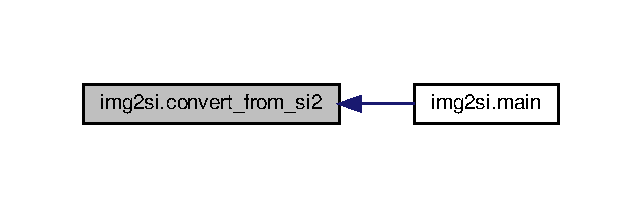
\includegraphics[width=308pt]{namespaceimg2si_a7c848960474f9c9e4beab3df12fb5e64_icgraph}
\end{center}
\end{figure}
\mbox{\Hypertarget{namespaceimg2si_a792ee72a74ed7abaf28cb4cc1d46869c}\label{namespaceimg2si_a792ee72a74ed7abaf28cb4cc1d46869c}} 
\index{img2si@{img2si}!convert\+\_\+to\+\_\+si2@{convert\+\_\+to\+\_\+si2}}
\index{convert\+\_\+to\+\_\+si2@{convert\+\_\+to\+\_\+si2}!img2si@{img2si}}
\subsubsection{\texorpdfstring{convert\+\_\+to\+\_\+si2()}{convert\_to\_si2()}}
{\footnotesize\ttfamily def img2si.\+convert\+\_\+to\+\_\+si2 (\begin{DoxyParamCaption}\item[{}]{source,  }\item[{}]{output }\end{DoxyParamCaption})}



Definition at line 59 of file img2si.\+py.

Here is the caller graph for this function\+:\nopagebreak
\begin{figure}[H]
\begin{center}
\leavevmode
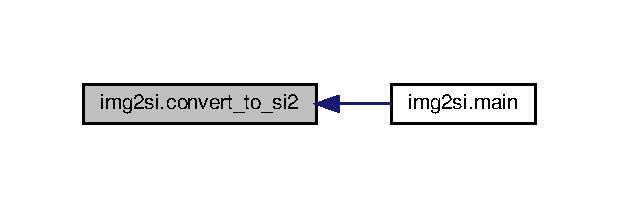
\includegraphics[width=297pt]{namespaceimg2si_a792ee72a74ed7abaf28cb4cc1d46869c_icgraph}
\end{center}
\end{figure}
\mbox{\Hypertarget{namespaceimg2si_a30df945259118023030181e530c9f6df}\label{namespaceimg2si_a30df945259118023030181e530c9f6df}} 
\index{img2si@{img2si}!is\+\_\+file\+\_\+si2@{is\+\_\+file\+\_\+si2}}
\index{is\+\_\+file\+\_\+si2@{is\+\_\+file\+\_\+si2}!img2si@{img2si}}
\subsubsection{\texorpdfstring{is\+\_\+file\+\_\+si2()}{is\_file\_si2()}}
{\footnotesize\ttfamily def img2si.\+is\+\_\+file\+\_\+si2 (\begin{DoxyParamCaption}\item[{}]{file\+Path }\end{DoxyParamCaption})}



Definition at line 28 of file img2si.\+py.

Here is the caller graph for this function\+:\nopagebreak
\begin{figure}[H]
\begin{center}
\leavevmode
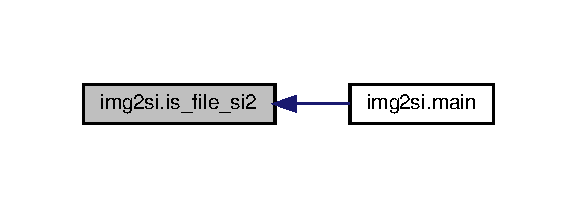
\includegraphics[width=277pt]{namespaceimg2si_a30df945259118023030181e530c9f6df_icgraph}
\end{center}
\end{figure}
\mbox{\Hypertarget{namespaceimg2si_a87146d74b97186b359e4b3572eaec249}\label{namespaceimg2si_a87146d74b97186b359e4b3572eaec249}} 
\index{img2si@{img2si}!main@{main}}
\index{main@{main}!img2si@{img2si}}
\subsubsection{\texorpdfstring{main()}{main()}}
{\footnotesize\ttfamily def img2si.\+main (\begin{DoxyParamCaption}{ }\end{DoxyParamCaption})}



Definition at line 95 of file img2si.\+py.

Here is the call graph for this function\+:\nopagebreak
\begin{figure}[H]
\begin{center}
\leavevmode
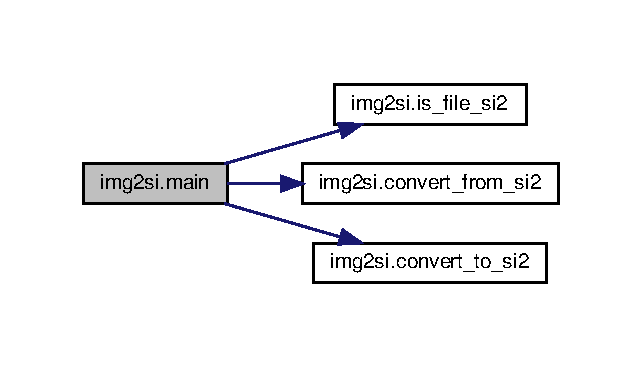
\includegraphics[width=308pt]{namespaceimg2si_a87146d74b97186b359e4b3572eaec249_cgraph}
\end{center}
\end{figure}

\hypertarget{namespacens_game}{}\section{ns\+Game Namespace Reference}
\label{namespacens_game}\index{ns\+Game@{ns\+Game}}
\subsection*{Classes}
\begin{DoxyCompactItemize}
\item 
class \hyperlink{classns_game_1_1_animation}{Animation}
\begin{DoxyCompactList}\small\item\em Defines animations. \end{DoxyCompactList}\item 
class \hyperlink{classns_game_1_1_cookie}{Cookie}
\begin{DoxyCompactList}\small\item\em Defines Food. \end{DoxyCompactList}\item 
class \hyperlink{classns_game_1_1_cooldowns}{Cooldowns}
\item 
class \hyperlink{structns_game_1_1_entity}{Entity}
\begin{DoxyCompactList}\small\item\em Defines the \hyperlink{structns_game_1_1_entity}{Entity} class. \end{DoxyCompactList}\item 
class \hyperlink{classns_game_1_1_fruit}{Fruit}
\begin{DoxyCompactList}\small\item\em Defines \hyperlink{classns_game_1_1_fruit}{Fruit}. \end{DoxyCompactList}\item 
class \hyperlink{classns_game_1_1_game_state}{Game\+State}
\begin{DoxyCompactList}\small\item\em Defines the game logic. \end{DoxyCompactList}\item 
class \hyperlink{structns_game_1_1_item}{Item}
\begin{DoxyCompactList}\small\item\em Defines the \hyperlink{structns_game_1_1_item}{Item}. \end{DoxyCompactList}\item 
class \hyperlink{classns_game_1_1_map}{Map}
\begin{DoxyCompactList}\small\item\em Defines the game grid, its textures, file loading, coordinates, positions. \end{DoxyCompactList}\item 
class \hyperlink{classns_game_1_1_monster}{Monster}
\begin{DoxyCompactList}\small\item\em Defines the monsters class. \end{DoxyCompactList}\item 
class \hyperlink{classns_game_1_1_player}{Player}
\begin{DoxyCompactList}\small\item\em Defines the player\textquotesingle{}s class. \end{DoxyCompactList}\item 
class \hyperlink{classns_game_1_1_powerup}{Powerup}
\begin{DoxyCompactList}\small\item\em Defines \hyperlink{classns_game_1_1_powerup}{Powerup} -\/ allows Pacman to eat monsters and players without getting killed. \end{DoxyCompactList}\item 
class \hyperlink{structns_game_1_1_state}{State}
\begin{DoxyCompactList}\small\item\em A class defining the different states of the game (In-\/game, Menus, Loading...) \end{DoxyCompactList}\item 
class \hyperlink{classns_game_1_1_state_manager}{State\+Manager}
\begin{DoxyCompactList}\small\item\em The class handling the game states. \end{DoxyCompactList}\end{DoxyCompactItemize}
\subsection*{Enumerations}
\begin{DoxyCompactItemize}
\item 
enum \hyperlink{namespacens_game_afea521dd2ba8e97be9549ce9936f4522}{Effect\+Type} \{ \hyperlink{namespacens_game_afea521dd2ba8e97be9549ce9936f4522ad8419bc5aa898e494274288a9ac80024}{I\+N\+V\+I\+N\+C\+I\+B\+LE}, 
\hyperlink{namespacens_game_afea521dd2ba8e97be9549ce9936f4522a3fb98417363f58fdca3c1736cb2bc524}{P\+O\+W\+ER}
 \}\begin{DoxyCompactList}\small\item\em The Effect\+Type enum. \end{DoxyCompactList}
\item 
enum \hyperlink{namespacens_game_a5f7db01e6447720e9a145f0b3c68a4d7}{Item\+Type} \{ \hyperlink{namespacens_game_a5f7db01e6447720e9a145f0b3c68a4d7af9fff3d8a5eecce5e7a5832384af32c7}{I\+T\+EM}, 
\hyperlink{namespacens_game_a5f7db01e6447720e9a145f0b3c68a4d7a4854f9b87edf18fbc6f4e3b5203e82fe}{F\+O\+OD}, 
\hyperlink{namespacens_game_a5f7db01e6447720e9a145f0b3c68a4d7a11fef96488a5f7c7890a7e4a55c44ec9}{F\+R\+U\+IT}, 
\hyperlink{namespacens_game_a5f7db01e6447720e9a145f0b3c68a4d7a8f64a06aec54275dc5b48f16ed3434d2}{P\+O\+W\+E\+R\+UP}
 \}\begin{DoxyCompactList}\small\item\em The Item\+Type enum. \end{DoxyCompactList}
\end{DoxyCompactItemize}


\subsection{Enumeration Type Documentation}
\mbox{\Hypertarget{namespacens_game_afea521dd2ba8e97be9549ce9936f4522}\label{namespacens_game_afea521dd2ba8e97be9549ce9936f4522}} 
\index{ns\+Game@{ns\+Game}!Effect\+Type@{Effect\+Type}}
\index{Effect\+Type@{Effect\+Type}!ns\+Game@{ns\+Game}}
\subsubsection{\texorpdfstring{Effect\+Type}{EffectType}}
{\footnotesize\ttfamily enum \hyperlink{namespacens_game_afea521dd2ba8e97be9549ce9936f4522}{ns\+Game\+::\+Effect\+Type}}



The Effect\+Type enum. 

\begin{DoxyEnumFields}{Enumerator}
\raisebox{\heightof{T}}[0pt][0pt]{\index{I\+N\+V\+I\+N\+C\+I\+B\+LE@{I\+N\+V\+I\+N\+C\+I\+B\+LE}!ns\+Game@{ns\+Game}}\index{ns\+Game@{ns\+Game}!I\+N\+V\+I\+N\+C\+I\+B\+LE@{I\+N\+V\+I\+N\+C\+I\+B\+LE}}}\mbox{\Hypertarget{namespacens_game_afea521dd2ba8e97be9549ce9936f4522ad8419bc5aa898e494274288a9ac80024}\label{namespacens_game_afea521dd2ba8e97be9549ce9936f4522ad8419bc5aa898e494274288a9ac80024}} 
I\+N\+V\+I\+N\+C\+I\+B\+LE&\\
\hline

\raisebox{\heightof{T}}[0pt][0pt]{\index{P\+O\+W\+ER@{P\+O\+W\+ER}!ns\+Game@{ns\+Game}}\index{ns\+Game@{ns\+Game}!P\+O\+W\+ER@{P\+O\+W\+ER}}}\mbox{\Hypertarget{namespacens_game_afea521dd2ba8e97be9549ce9936f4522a3fb98417363f58fdca3c1736cb2bc524}\label{namespacens_game_afea521dd2ba8e97be9549ce9936f4522a3fb98417363f58fdca3c1736cb2bc524}} 
P\+O\+W\+ER&\\
\hline

\end{DoxyEnumFields}


Definition at line 16 of file effect\+Type.\+h.

\mbox{\Hypertarget{namespacens_game_a5f7db01e6447720e9a145f0b3c68a4d7}\label{namespacens_game_a5f7db01e6447720e9a145f0b3c68a4d7}} 
\index{ns\+Game@{ns\+Game}!Item\+Type@{Item\+Type}}
\index{Item\+Type@{Item\+Type}!ns\+Game@{ns\+Game}}
\subsubsection{\texorpdfstring{Item\+Type}{ItemType}}
{\footnotesize\ttfamily enum \hyperlink{namespacens_game_a5f7db01e6447720e9a145f0b3c68a4d7}{ns\+Game\+::\+Item\+Type}}



The Item\+Type enum. 

\begin{DoxyEnumFields}{Enumerator}
\raisebox{\heightof{T}}[0pt][0pt]{\index{I\+T\+EM@{I\+T\+EM}!ns\+Game@{ns\+Game}}\index{ns\+Game@{ns\+Game}!I\+T\+EM@{I\+T\+EM}}}\mbox{\Hypertarget{namespacens_game_a5f7db01e6447720e9a145f0b3c68a4d7af9fff3d8a5eecce5e7a5832384af32c7}\label{namespacens_game_a5f7db01e6447720e9a145f0b3c68a4d7af9fff3d8a5eecce5e7a5832384af32c7}} 
I\+T\+EM&\\
\hline

\raisebox{\heightof{T}}[0pt][0pt]{\index{F\+O\+OD@{F\+O\+OD}!ns\+Game@{ns\+Game}}\index{ns\+Game@{ns\+Game}!F\+O\+OD@{F\+O\+OD}}}\mbox{\Hypertarget{namespacens_game_a5f7db01e6447720e9a145f0b3c68a4d7a4854f9b87edf18fbc6f4e3b5203e82fe}\label{namespacens_game_a5f7db01e6447720e9a145f0b3c68a4d7a4854f9b87edf18fbc6f4e3b5203e82fe}} 
F\+O\+OD&\\
\hline

\raisebox{\heightof{T}}[0pt][0pt]{\index{F\+R\+U\+IT@{F\+R\+U\+IT}!ns\+Game@{ns\+Game}}\index{ns\+Game@{ns\+Game}!F\+R\+U\+IT@{F\+R\+U\+IT}}}\mbox{\Hypertarget{namespacens_game_a5f7db01e6447720e9a145f0b3c68a4d7a11fef96488a5f7c7890a7e4a55c44ec9}\label{namespacens_game_a5f7db01e6447720e9a145f0b3c68a4d7a11fef96488a5f7c7890a7e4a55c44ec9}} 
F\+R\+U\+IT&\\
\hline

\raisebox{\heightof{T}}[0pt][0pt]{\index{P\+O\+W\+E\+R\+UP@{P\+O\+W\+E\+R\+UP}!ns\+Game@{ns\+Game}}\index{ns\+Game@{ns\+Game}!P\+O\+W\+E\+R\+UP@{P\+O\+W\+E\+R\+UP}}}\mbox{\Hypertarget{namespacens_game_a5f7db01e6447720e9a145f0b3c68a4d7a8f64a06aec54275dc5b48f16ed3434d2}\label{namespacens_game_a5f7db01e6447720e9a145f0b3c68a4d7a8f64a06aec54275dc5b48f16ed3434d2}} 
P\+O\+W\+E\+R\+UP&\\
\hline

\end{DoxyEnumFields}


Definition at line 19 of file item.\+h.


\chapter{Class Documentation}
\hypertarget{classns_game_1_1_animation}{}\section{ns\+Game\+:\+:Animation Class Reference}
\label{classns_game_1_1_animation}\index{ns\+Game\+::\+Animation@{ns\+Game\+::\+Animation}}


Defines animations.  




{\ttfamily \#include $<$animation.\+h$>$}

\subsection*{Public Member Functions}
\begin{DoxyCompactItemize}
\item 
\hyperlink{classns_game_1_1_animation_aebaabfa10569678e6a7d30fa9c8d031d}{Animation} ()
\item 
\hyperlink{classns_game_1_1_animation_a0554455321614f3f94bbcbd5b784cfd5}{Animation} (ns\+Graphics\+::\+Vec2D pos)
\item 
\hyperlink{classns_game_1_1_animation_a022c8e1738aee4ce2e2c15abbeedc711}{Animation} (unsigned \hyperlink{classns_game_1_1_animation_abde2f282d6d865a253f0a6edc0964508}{delay}, bool \hyperlink{classns_game_1_1_animation_a3f119a84e6993f0676c9cde2b84a61dd}{alternate})
\item 
\hyperlink{classns_game_1_1_animation_a0170b0eeb1b1f41d4f0a5270877e9897}{Animation} (unsigned \hyperlink{classns_game_1_1_animation_abde2f282d6d865a253f0a6edc0964508}{delay}, bool \hyperlink{classns_game_1_1_animation_a3f119a84e6993f0676c9cde2b84a61dd}{alternate}, ns\+Graphics\+::\+Vec2D pos)
\item 
void \hyperlink{classns_game_1_1_animation_a5f32b1fc6ad5d228a4153d7421fa457b}{update} (unsigned delta)
\begin{DoxyCompactList}\small\item\em Updates animation, changes sprite according to delta and direction. \end{DoxyCompactList}\item 
void \hyperlink{classns_game_1_1_animation_a626733cd1a3031caf438b656f1d805cd}{set\+Coordinates} (int x, int y)
\begin{DoxyCompactList}\small\item\em Sets coordinates on the window. \end{DoxyCompactList}\item 
void \hyperlink{classns_game_1_1_animation_a1a103b09407581b74933001fb8b3a8f0}{set\+Position} (int x, int y)
\begin{DoxyCompactList}\small\item\em Sets position on the map. \end{DoxyCompactList}\item 
void \hyperlink{classns_game_1_1_animation_a2dc40787df4708e3f5d81e5529595574}{set\+Position} (ns\+Graphics\+::\+Vec2D pos)
\begin{DoxyCompactList}\small\item\em Sets position on the map. \end{DoxyCompactList}\item 
void \hyperlink{classns_game_1_1_animation_a348e25058d77891160c015da88ea4837}{render} (Min\+GL \&window)
\begin{DoxyCompactList}\small\item\em Renders resources. \end{DoxyCompactList}\end{DoxyCompactItemize}
\subsection*{Public Attributes}
\begin{DoxyCompactItemize}
\item 
unsigned \hyperlink{classns_game_1_1_animation_abde2f282d6d865a253f0a6edc0964508}{delay} = 500
\begin{DoxyCompactList}\small\item\em Delay between frames. \end{DoxyCompactList}\item 
unsigned \hyperlink{classns_game_1_1_animation_a2cb68d312de6b044102c6a1e65221eb3}{current\+Sprite} = 0
\item 
bool \hyperlink{classns_game_1_1_animation_a3f119a84e6993f0676c9cde2b84a61dd}{alternate} = true
\begin{DoxyCompactList}\small\item\em Allows animation to go from start to end, then end to start, and vice versa. \end{DoxyCompactList}\item 
std\+::vector$<$ ns\+Gui\+::\+Sprite $>$ \hyperlink{classns_game_1_1_animation_a1757a8a9ce0a3fc6a75b1289b78753bb}{sprites}
\begin{DoxyCompactList}\small\item\em Sprites list. \end{DoxyCompactList}\end{DoxyCompactItemize}


\subsection{Detailed Description}
Defines animations. 

\begin{DoxyAuthor}{Author}
Thomas Cardon 
\end{DoxyAuthor}


Definition at line 20 of file animation.\+h.



\subsection{Constructor \& Destructor Documentation}
\mbox{\Hypertarget{classns_game_1_1_animation_aebaabfa10569678e6a7d30fa9c8d031d}\label{classns_game_1_1_animation_aebaabfa10569678e6a7d30fa9c8d031d}} 
\index{ns\+Game\+::\+Animation@{ns\+Game\+::\+Animation}!Animation@{Animation}}
\index{Animation@{Animation}!ns\+Game\+::\+Animation@{ns\+Game\+::\+Animation}}
\subsubsection{\texorpdfstring{Animation()}{Animation()}\hspace{0.1cm}{\footnotesize\ttfamily [1/4]}}
{\footnotesize\ttfamily ns\+Game\+::\+Animation\+::\+Animation (\begin{DoxyParamCaption}{ }\end{DoxyParamCaption})}

\mbox{\Hypertarget{classns_game_1_1_animation_a0554455321614f3f94bbcbd5b784cfd5}\label{classns_game_1_1_animation_a0554455321614f3f94bbcbd5b784cfd5}} 
\index{ns\+Game\+::\+Animation@{ns\+Game\+::\+Animation}!Animation@{Animation}}
\index{Animation@{Animation}!ns\+Game\+::\+Animation@{ns\+Game\+::\+Animation}}
\subsubsection{\texorpdfstring{Animation()}{Animation()}\hspace{0.1cm}{\footnotesize\ttfamily [2/4]}}
{\footnotesize\ttfamily Animation\+::\+Animation (\begin{DoxyParamCaption}\item[{ns\+Graphics\+::\+Vec2D}]{pos }\end{DoxyParamCaption})}



Definition at line 13 of file animation.\+cpp.

\mbox{\Hypertarget{classns_game_1_1_animation_a022c8e1738aee4ce2e2c15abbeedc711}\label{classns_game_1_1_animation_a022c8e1738aee4ce2e2c15abbeedc711}} 
\index{ns\+Game\+::\+Animation@{ns\+Game\+::\+Animation}!Animation@{Animation}}
\index{Animation@{Animation}!ns\+Game\+::\+Animation@{ns\+Game\+::\+Animation}}
\subsubsection{\texorpdfstring{Animation()}{Animation()}\hspace{0.1cm}{\footnotesize\ttfamily [3/4]}}
{\footnotesize\ttfamily Animation\+::\+Animation (\begin{DoxyParamCaption}\item[{unsigned}]{delay,  }\item[{bool}]{alternate }\end{DoxyParamCaption})}



Definition at line 17 of file animation.\+cpp.

\mbox{\Hypertarget{classns_game_1_1_animation_a0170b0eeb1b1f41d4f0a5270877e9897}\label{classns_game_1_1_animation_a0170b0eeb1b1f41d4f0a5270877e9897}} 
\index{ns\+Game\+::\+Animation@{ns\+Game\+::\+Animation}!Animation@{Animation}}
\index{Animation@{Animation}!ns\+Game\+::\+Animation@{ns\+Game\+::\+Animation}}
\subsubsection{\texorpdfstring{Animation()}{Animation()}\hspace{0.1cm}{\footnotesize\ttfamily [4/4]}}
{\footnotesize\ttfamily Animation\+::\+Animation (\begin{DoxyParamCaption}\item[{unsigned}]{delay,  }\item[{bool}]{alternate,  }\item[{ns\+Graphics\+::\+Vec2D}]{pos }\end{DoxyParamCaption})}



Definition at line 22 of file animation.\+cpp.



\subsection{Member Function Documentation}
\mbox{\Hypertarget{classns_game_1_1_animation_a348e25058d77891160c015da88ea4837}\label{classns_game_1_1_animation_a348e25058d77891160c015da88ea4837}} 
\index{ns\+Game\+::\+Animation@{ns\+Game\+::\+Animation}!render@{render}}
\index{render@{render}!ns\+Game\+::\+Animation@{ns\+Game\+::\+Animation}}
\subsubsection{\texorpdfstring{render()}{render()}}
{\footnotesize\ttfamily void ns\+Game\+::\+Animation\+::render (\begin{DoxyParamCaption}\item[{Min\+GL \&}]{window }\end{DoxyParamCaption})}



Renders resources. 



Definition at line 61 of file animation.\+cpp.

Here is the caller graph for this function\+:\nopagebreak
\begin{figure}[H]
\begin{center}
\leavevmode
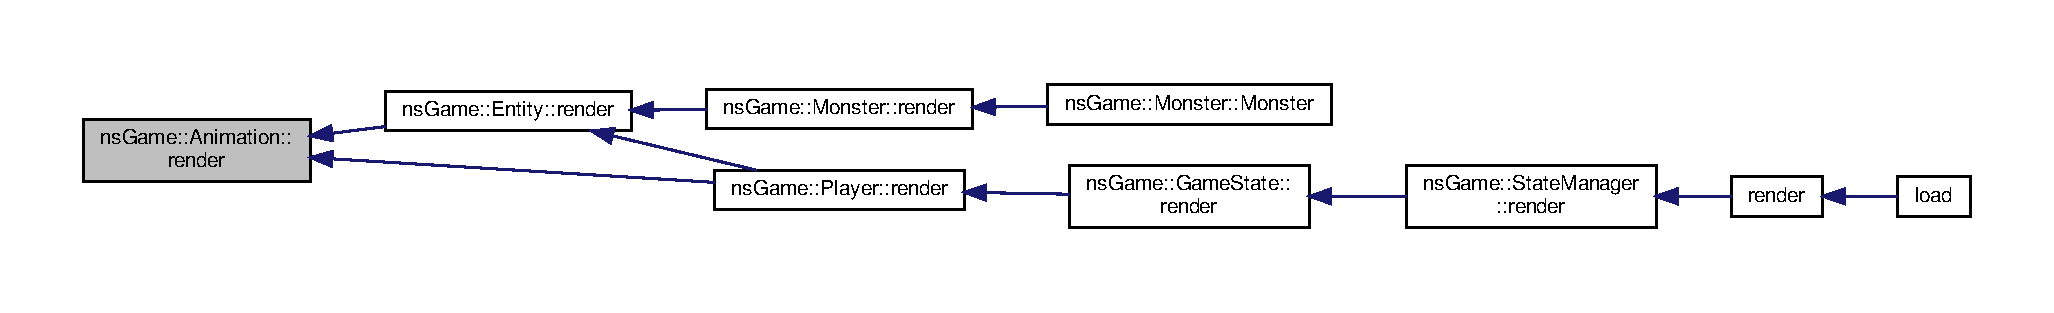
\includegraphics[width=350pt]{classns_game_1_1_animation_a348e25058d77891160c015da88ea4837_icgraph}
\end{center}
\end{figure}
\mbox{\Hypertarget{classns_game_1_1_animation_a626733cd1a3031caf438b656f1d805cd}\label{classns_game_1_1_animation_a626733cd1a3031caf438b656f1d805cd}} 
\index{ns\+Game\+::\+Animation@{ns\+Game\+::\+Animation}!set\+Coordinates@{set\+Coordinates}}
\index{set\+Coordinates@{set\+Coordinates}!ns\+Game\+::\+Animation@{ns\+Game\+::\+Animation}}
\subsubsection{\texorpdfstring{set\+Coordinates()}{setCoordinates()}}
{\footnotesize\ttfamily void ns\+Game\+::\+Animation\+::set\+Coordinates (\begin{DoxyParamCaption}\item[{int}]{x,  }\item[{int}]{y }\end{DoxyParamCaption})}



Sets coordinates on the window. 



Definition at line 47 of file animation.\+cpp.

\mbox{\Hypertarget{classns_game_1_1_animation_a1a103b09407581b74933001fb8b3a8f0}\label{classns_game_1_1_animation_a1a103b09407581b74933001fb8b3a8f0}} 
\index{ns\+Game\+::\+Animation@{ns\+Game\+::\+Animation}!set\+Position@{set\+Position}}
\index{set\+Position@{set\+Position}!ns\+Game\+::\+Animation@{ns\+Game\+::\+Animation}}
\subsubsection{\texorpdfstring{set\+Position()}{setPosition()}\hspace{0.1cm}{\footnotesize\ttfamily [1/2]}}
{\footnotesize\ttfamily ns\+Game\+::\+Animation\+::set\+Position (\begin{DoxyParamCaption}\item[{int}]{x,  }\item[{int}]{y }\end{DoxyParamCaption})}



Sets position on the map. 



Definition at line 56 of file animation.\+cpp.

Here is the caller graph for this function\+:\nopagebreak
\begin{figure}[H]
\begin{center}
\leavevmode
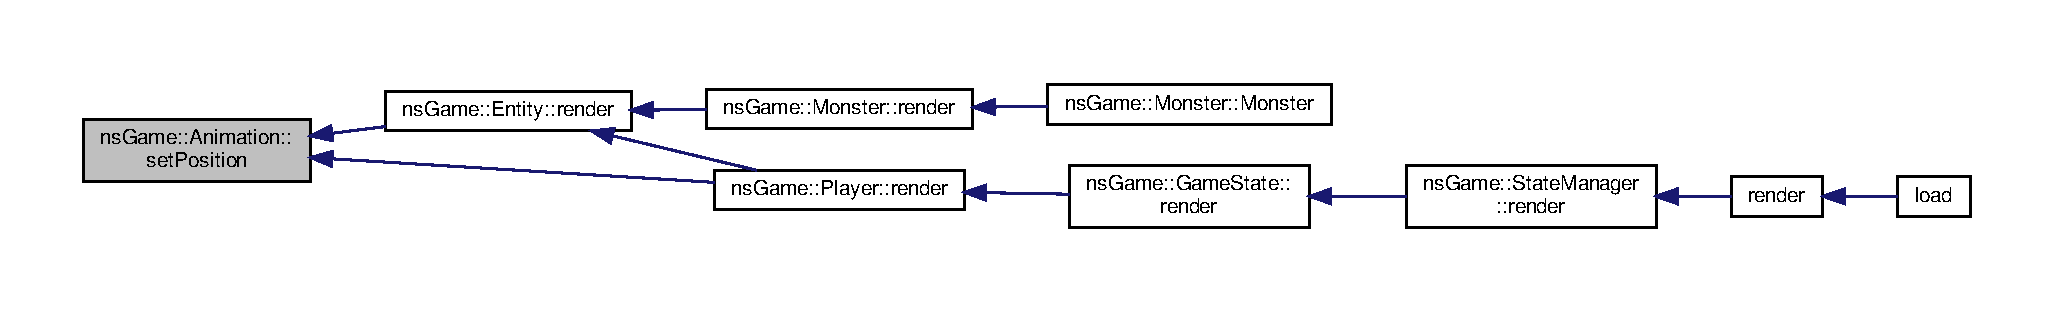
\includegraphics[width=350pt]{classns_game_1_1_animation_a1a103b09407581b74933001fb8b3a8f0_icgraph}
\end{center}
\end{figure}
\mbox{\Hypertarget{classns_game_1_1_animation_a2dc40787df4708e3f5d81e5529595574}\label{classns_game_1_1_animation_a2dc40787df4708e3f5d81e5529595574}} 
\index{ns\+Game\+::\+Animation@{ns\+Game\+::\+Animation}!set\+Position@{set\+Position}}
\index{set\+Position@{set\+Position}!ns\+Game\+::\+Animation@{ns\+Game\+::\+Animation}}
\subsubsection{\texorpdfstring{set\+Position()}{setPosition()}\hspace{0.1cm}{\footnotesize\ttfamily [2/2]}}
{\footnotesize\ttfamily ns\+Game\+::\+Animation\+::set\+Position (\begin{DoxyParamCaption}\item[{ns\+Graphics\+::\+Vec2D}]{pos }\end{DoxyParamCaption})}



Sets position on the map. 



Definition at line 52 of file animation.\+cpp.

\mbox{\Hypertarget{classns_game_1_1_animation_a5f32b1fc6ad5d228a4153d7421fa457b}\label{classns_game_1_1_animation_a5f32b1fc6ad5d228a4153d7421fa457b}} 
\index{ns\+Game\+::\+Animation@{ns\+Game\+::\+Animation}!update@{update}}
\index{update@{update}!ns\+Game\+::\+Animation@{ns\+Game\+::\+Animation}}
\subsubsection{\texorpdfstring{update()}{update()}}
{\footnotesize\ttfamily void ns\+Game\+::\+Animation\+::update (\begin{DoxyParamCaption}\item[{unsigned}]{delta }\end{DoxyParamCaption})}



Updates animation, changes sprite according to delta and direction. 



Definition at line 28 of file animation.\+cpp.

Here is the caller graph for this function\+:\nopagebreak
\begin{figure}[H]
\begin{center}
\leavevmode
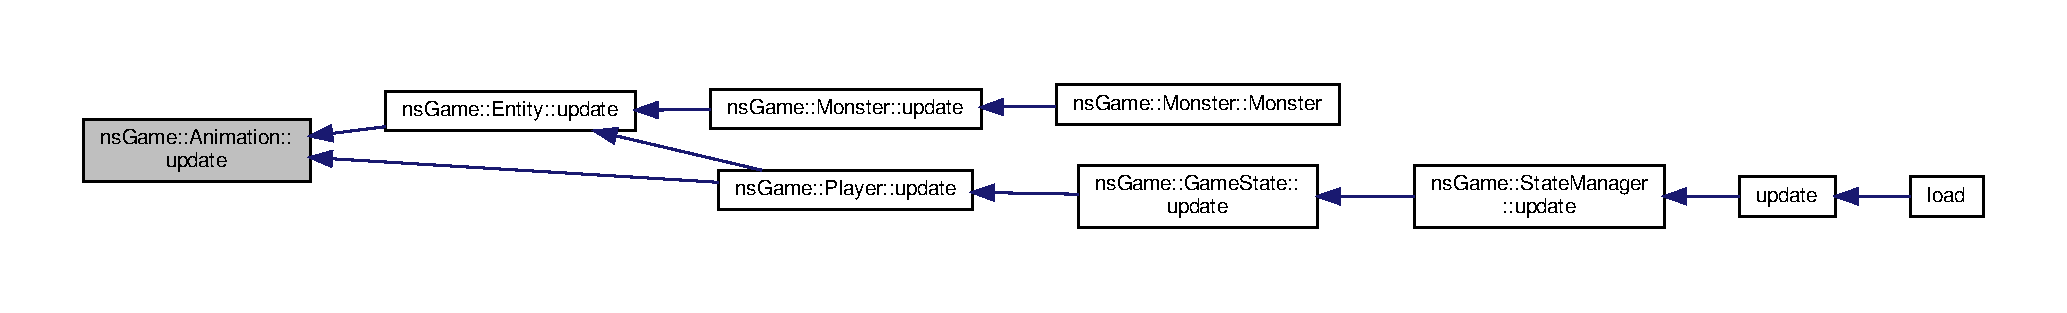
\includegraphics[width=350pt]{classns_game_1_1_animation_a5f32b1fc6ad5d228a4153d7421fa457b_icgraph}
\end{center}
\end{figure}


\subsection{Member Data Documentation}
\mbox{\Hypertarget{classns_game_1_1_animation_a3f119a84e6993f0676c9cde2b84a61dd}\label{classns_game_1_1_animation_a3f119a84e6993f0676c9cde2b84a61dd}} 
\index{ns\+Game\+::\+Animation@{ns\+Game\+::\+Animation}!alternate@{alternate}}
\index{alternate@{alternate}!ns\+Game\+::\+Animation@{ns\+Game\+::\+Animation}}
\subsubsection{\texorpdfstring{alternate}{alternate}}
{\footnotesize\ttfamily bool ns\+Game\+::\+Animation\+::alternate = true}



Allows animation to go from start to end, then end to start, and vice versa. 



Definition at line 39 of file animation.\+h.

\mbox{\Hypertarget{classns_game_1_1_animation_a2cb68d312de6b044102c6a1e65221eb3}\label{classns_game_1_1_animation_a2cb68d312de6b044102c6a1e65221eb3}} 
\index{ns\+Game\+::\+Animation@{ns\+Game\+::\+Animation}!current\+Sprite@{current\+Sprite}}
\index{current\+Sprite@{current\+Sprite}!ns\+Game\+::\+Animation@{ns\+Game\+::\+Animation}}
\subsubsection{\texorpdfstring{current\+Sprite}{currentSprite}}
{\footnotesize\ttfamily unsigned ns\+Game\+::\+Animation\+::current\+Sprite = 0}



Definition at line 36 of file animation.\+h.

\mbox{\Hypertarget{classns_game_1_1_animation_abde2f282d6d865a253f0a6edc0964508}\label{classns_game_1_1_animation_abde2f282d6d865a253f0a6edc0964508}} 
\index{ns\+Game\+::\+Animation@{ns\+Game\+::\+Animation}!delay@{delay}}
\index{delay@{delay}!ns\+Game\+::\+Animation@{ns\+Game\+::\+Animation}}
\subsubsection{\texorpdfstring{delay}{delay}}
{\footnotesize\ttfamily unsigned ns\+Game\+::\+Animation\+::delay = 500}



Delay between frames. 



Definition at line 36 of file animation.\+h.

\mbox{\Hypertarget{classns_game_1_1_animation_a1757a8a9ce0a3fc6a75b1289b78753bb}\label{classns_game_1_1_animation_a1757a8a9ce0a3fc6a75b1289b78753bb}} 
\index{ns\+Game\+::\+Animation@{ns\+Game\+::\+Animation}!sprites@{sprites}}
\index{sprites@{sprites}!ns\+Game\+::\+Animation@{ns\+Game\+::\+Animation}}
\subsubsection{\texorpdfstring{sprites}{sprites}}
{\footnotesize\ttfamily std\+::vector$<$ns\+Gui\+::\+Sprite$>$ ns\+Game\+::\+Animation\+::sprites}



Sprites list. 



Definition at line 42 of file animation.\+h.



The documentation for this class was generated from the following files\+:\begin{DoxyCompactItemize}
\item 
Nos\+\_\+fichiers/\hyperlink{animation_8h}{animation.\+h}\item 
Nos\+\_\+fichiers/\hyperlink{animation_8cpp}{animation.\+cpp}\end{DoxyCompactItemize}

\hypertarget{struct_authorized_key}{}\section{Authorized\+Key Struct Reference}
\label{struct_authorized_key}\index{Authorized\+Key@{Authorized\+Key}}


Struct containing all the authorized keys in the struct \hyperlink{struct_c_my_param}{C\+My\+Param}.  




{\ttfamily \#include $<$type.\+h$>$}

\subsection*{Public Attributes}
\begin{DoxyCompactItemize}
\item 
const std\+::vector$<$ std\+::string $>$ \hyperlink{struct_authorized_key_a1b1aa7863427cc1b43f229423bdd83ba}{V\+Param\+Char} \{\char`\"{}P1\+\_\+\+Key\+Up\char`\"{}, \char`\"{}P1\+\_\+\+Key\+Down\char`\"{}, \char`\"{}P1\+\_\+\+Key\+Left\char`\"{}, \char`\"{}P1\+\_\+\+Key\+Right\char`\"{}, \char`\"{}P1\+\_\+\+Key\+Action1\char`\"{}, \char`\"{}P2\+\_\+\+Key\+Up\char`\"{}, \char`\"{}P2\+\_\+\+Key\+Down\char`\"{}, \char`\"{}P2\+\_\+\+Key\+Left\char`\"{}, \char`\"{}P2\+\_\+\+Key\+Right\char`\"{}, \char`\"{}P2\+\_\+\+Key\+Action1\char`\"{}, \char`\"{}Token\+P1\char`\"{}, \char`\"{}Token\+P2\char`\"{}\}
\item 
const std\+::vector$<$ std\+::string $>$ \hyperlink{struct_authorized_key_a14d2cbd0e3dcc77a793a55f988d78b73}{V\+Param\+String} \{\}
\item 
const std\+::vector$<$ std\+::string $>$ \hyperlink{struct_authorized_key_a871173f4b0c89c91289a10f0ddc1cadd}{V\+Param\+Unsigned} \{\}
\end{DoxyCompactItemize}


\subsection{Detailed Description}
Struct containing all the authorized keys in the struct \hyperlink{struct_c_my_param}{C\+My\+Param}. 

Definition at line 61 of file type.\+h.



\subsection{Member Data Documentation}
\mbox{\Hypertarget{struct_authorized_key_a1b1aa7863427cc1b43f229423bdd83ba}\label{struct_authorized_key_a1b1aa7863427cc1b43f229423bdd83ba}} 
\index{Authorized\+Key@{Authorized\+Key}!V\+Param\+Char@{V\+Param\+Char}}
\index{V\+Param\+Char@{V\+Param\+Char}!Authorized\+Key@{Authorized\+Key}}
\subsubsection{\texorpdfstring{V\+Param\+Char}{VParamChar}}
{\footnotesize\ttfamily const std\+::vector$<$std\+::string$>$ Authorized\+Key\+::\+V\+Param\+Char \{\char`\"{}P1\+\_\+\+Key\+Up\char`\"{}, \char`\"{}P1\+\_\+\+Key\+Down\char`\"{}, \char`\"{}P1\+\_\+\+Key\+Left\char`\"{}, \char`\"{}P1\+\_\+\+Key\+Right\char`\"{}, \char`\"{}P1\+\_\+\+Key\+Action1\char`\"{}, \char`\"{}P2\+\_\+\+Key\+Up\char`\"{}, \char`\"{}P2\+\_\+\+Key\+Down\char`\"{}, \char`\"{}P2\+\_\+\+Key\+Left\char`\"{}, \char`\"{}P2\+\_\+\+Key\+Right\char`\"{}, \char`\"{}P2\+\_\+\+Key\+Action1\char`\"{}, \char`\"{}Token\+P1\char`\"{}, \char`\"{}Token\+P2\char`\"{}\}}

List of authorized key for the type char in a struct \hyperlink{struct_c_my_param}{C\+My\+Param} 

Definition at line 63 of file type.\+h.

\mbox{\Hypertarget{struct_authorized_key_a14d2cbd0e3dcc77a793a55f988d78b73}\label{struct_authorized_key_a14d2cbd0e3dcc77a793a55f988d78b73}} 
\index{Authorized\+Key@{Authorized\+Key}!V\+Param\+String@{V\+Param\+String}}
\index{V\+Param\+String@{V\+Param\+String}!Authorized\+Key@{Authorized\+Key}}
\subsubsection{\texorpdfstring{V\+Param\+String}{VParamString}}
{\footnotesize\ttfamily const std\+::vector$<$std\+::string$>$ Authorized\+Key\+::\+V\+Param\+String \{\}}

List of authorized key for the type string in a struct \hyperlink{struct_c_my_param}{C\+My\+Param} 

Definition at line 65 of file type.\+h.

\mbox{\Hypertarget{struct_authorized_key_a871173f4b0c89c91289a10f0ddc1cadd}\label{struct_authorized_key_a871173f4b0c89c91289a10f0ddc1cadd}} 
\index{Authorized\+Key@{Authorized\+Key}!V\+Param\+Unsigned@{V\+Param\+Unsigned}}
\index{V\+Param\+Unsigned@{V\+Param\+Unsigned}!Authorized\+Key@{Authorized\+Key}}
\subsubsection{\texorpdfstring{V\+Param\+Unsigned}{VParamUnsigned}}
{\footnotesize\ttfamily const std\+::vector$<$std\+::string$>$ Authorized\+Key\+::\+V\+Param\+Unsigned \{\}}

List of authorized key for the type unsigned in a struct \hyperlink{struct_c_my_param}{C\+My\+Param} 

Definition at line 67 of file type.\+h.



The documentation for this struct was generated from the following file\+:\begin{DoxyCompactItemize}
\item 
Nos\+\_\+fichiers/\hyperlink{type_8h}{type.\+h}\end{DoxyCompactItemize}

\hypertarget{struct_c_my_param}{}\section{C\+My\+Param Struct Reference}
\label{struct_c_my_param}\index{C\+My\+Param@{C\+My\+Param}}


Struct containing all the game\textquotesingle{}s parameters.  




{\ttfamily \#include $<$type.\+h$>$}

\subsection*{Public Attributes}
\begin{DoxyCompactItemize}
\item 
std\+::map$<$ std\+::string, char $>$ \hyperlink{struct_c_my_param_ac38ede5a509bd268e749bc9c960466d3}{Map\+Param\+Char}
\item 
std\+::map$<$ std\+::string, unsigned $>$ \hyperlink{struct_c_my_param_aece7d4bdf4103e359f769d08e97a459d}{Map\+Param\+Unsigned}
\item 
std\+::map$<$ std\+::string, std\+::string $>$ \hyperlink{struct_c_my_param_a6f22660b5eff76608f47c52930e6ecf1}{Map\+Param\+String}
\end{DoxyCompactItemize}


\subsection{Detailed Description}
Struct containing all the game\textquotesingle{}s parameters. 

Definition at line 49 of file type.\+h.



\subsection{Member Data Documentation}
\mbox{\Hypertarget{struct_c_my_param_ac38ede5a509bd268e749bc9c960466d3}\label{struct_c_my_param_ac38ede5a509bd268e749bc9c960466d3}} 
\index{C\+My\+Param@{C\+My\+Param}!Map\+Param\+Char@{Map\+Param\+Char}}
\index{Map\+Param\+Char@{Map\+Param\+Char}!C\+My\+Param@{C\+My\+Param}}
\subsubsection{\texorpdfstring{Map\+Param\+Char}{MapParamChar}}
{\footnotesize\ttfamily std\+::map$<$std\+::string, char$>$ C\+My\+Param\+::\+Map\+Param\+Char}

List of parameters of type char 

Definition at line 51 of file type.\+h.

\mbox{\Hypertarget{struct_c_my_param_a6f22660b5eff76608f47c52930e6ecf1}\label{struct_c_my_param_a6f22660b5eff76608f47c52930e6ecf1}} 
\index{C\+My\+Param@{C\+My\+Param}!Map\+Param\+String@{Map\+Param\+String}}
\index{Map\+Param\+String@{Map\+Param\+String}!C\+My\+Param@{C\+My\+Param}}
\subsubsection{\texorpdfstring{Map\+Param\+String}{MapParamString}}
{\footnotesize\ttfamily std\+::map$<$std\+::string, std\+::string$>$ C\+My\+Param\+::\+Map\+Param\+String}

List of parameters of type string 

Definition at line 55 of file type.\+h.

\mbox{\Hypertarget{struct_c_my_param_aece7d4bdf4103e359f769d08e97a459d}\label{struct_c_my_param_aece7d4bdf4103e359f769d08e97a459d}} 
\index{C\+My\+Param@{C\+My\+Param}!Map\+Param\+Unsigned@{Map\+Param\+Unsigned}}
\index{Map\+Param\+Unsigned@{Map\+Param\+Unsigned}!C\+My\+Param@{C\+My\+Param}}
\subsubsection{\texorpdfstring{Map\+Param\+Unsigned}{MapParamUnsigned}}
{\footnotesize\ttfamily std\+::map$<$std\+::string, unsigned$>$ C\+My\+Param\+::\+Map\+Param\+Unsigned}

List of parameters of type unsigned 

Definition at line 53 of file type.\+h.



The documentation for this struct was generated from the following file\+:\begin{DoxyCompactItemize}
\item 
Nos\+\_\+fichiers/\hyperlink{type_8h}{type.\+h}\end{DoxyCompactItemize}

\hypertarget{classns_game_1_1_cookie}{}\section{ns\+Game\+:\+:Cookie Class Reference}
\label{classns_game_1_1_cookie}\index{ns\+Game\+::\+Cookie@{ns\+Game\+::\+Cookie}}


Defines Food.  




{\ttfamily \#include $<$cookie.\+h$>$}



Inheritance diagram for ns\+Game\+:\+:Cookie\+:\nopagebreak
\begin{figure}[H]
\begin{center}
\leavevmode
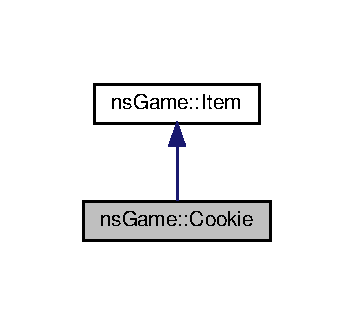
\includegraphics[width=170pt]{classns_game_1_1_cookie__inherit__graph}
\end{center}
\end{figure}


Collaboration diagram for ns\+Game\+:\+:Cookie\+:\nopagebreak
\begin{figure}[H]
\begin{center}
\leavevmode
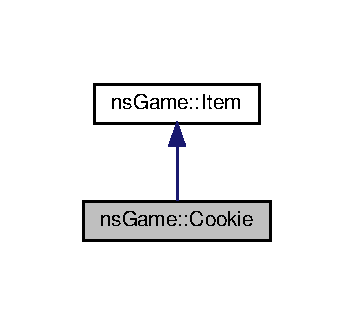
\includegraphics[width=170pt]{classns_game_1_1_cookie__coll__graph}
\end{center}
\end{figure}
\subsection*{Public Member Functions}
\begin{DoxyCompactItemize}
\item 
\hyperlink{classns_game_1_1_cookie_a2e6c34dfd2892c48dc4ce2b503504674}{Cookie} (ns\+Graphics\+::\+Vec2D \hyperlink{structns_game_1_1_item_a5518876a13f3d2eda659d29748097f1a}{pos})
\item 
ns\+Graphics\+::\+Vec2D \hyperlink{classns_game_1_1_cookie_ab624101d018f74fb856bdfd7fd97c55e}{get\+Coordinates} ()
\begin{DoxyCompactList}\small\item\em This function is used to get the position on the screen/canvas/window, whatever you want to call it. \end{DoxyCompactList}\item 
void \hyperlink{classns_game_1_1_cookie_a20769adf2b327f4bf519e851073b1891}{load} () override
\begin{DoxyCompactList}\small\item\em Loads food. \end{DoxyCompactList}\item 
void \hyperlink{classns_game_1_1_cookie_aaea5c3967effe908f2676a5ded17aa39}{update} (unsigned delta) override
\begin{DoxyCompactList}\small\item\em Updates food. \end{DoxyCompactList}\item 
void \hyperlink{classns_game_1_1_cookie_a7e321497bf9d9baa738d987e9c47dd5e}{render} (Min\+GL \&window) override
\begin{DoxyCompactList}\small\item\em Renders resources. \end{DoxyCompactList}\item 
void \hyperlink{classns_game_1_1_cookie_a2cd4ee8c83b99191643d6e9ef2267b1a}{action} (\hyperlink{classns_game_1_1_player}{Player} $\ast$player) override
\begin{DoxyCompactList}\small\item\em Makes an action for the player. \end{DoxyCompactList}\item 
\hyperlink{namespacens_game_a5f7db01e6447720e9a145f0b3c68a4d7}{Item\+Type} \hyperlink{classns_game_1_1_cookie_ac5c28f610947708bc1f31b1e8a88ef42}{get\+Type} () override
\begin{DoxyCompactList}\small\item\em Gets item type. \end{DoxyCompactList}\end{DoxyCompactItemize}
\subsection*{Additional Inherited Members}


\subsection{Detailed Description}
Defines Food. 

\begin{DoxyAuthor}{Authors}
Thomas Cardon 
\end{DoxyAuthor}


Definition at line 23 of file cookie.\+h.



\subsection{Constructor \& Destructor Documentation}
\mbox{\Hypertarget{classns_game_1_1_cookie_a2e6c34dfd2892c48dc4ce2b503504674}\label{classns_game_1_1_cookie_a2e6c34dfd2892c48dc4ce2b503504674}} 
\index{ns\+Game\+::\+Cookie@{ns\+Game\+::\+Cookie}!Cookie@{Cookie}}
\index{Cookie@{Cookie}!ns\+Game\+::\+Cookie@{ns\+Game\+::\+Cookie}}
\subsubsection{\texorpdfstring{Cookie()}{Cookie()}}
{\footnotesize\ttfamily ns\+Game\+::\+Cookie\+::\+Cookie (\begin{DoxyParamCaption}\item[{ns\+Graphics\+::\+Vec2D}]{pos }\end{DoxyParamCaption})\hspace{0.3cm}{\ttfamily [inline]}}



Definition at line 26 of file cookie.\+h.



\subsection{Member Function Documentation}
\mbox{\Hypertarget{classns_game_1_1_cookie_a2cd4ee8c83b99191643d6e9ef2267b1a}\label{classns_game_1_1_cookie_a2cd4ee8c83b99191643d6e9ef2267b1a}} 
\index{ns\+Game\+::\+Cookie@{ns\+Game\+::\+Cookie}!action@{action}}
\index{action@{action}!ns\+Game\+::\+Cookie@{ns\+Game\+::\+Cookie}}
\subsubsection{\texorpdfstring{action()}{action()}}
{\footnotesize\ttfamily void Cookie\+::action (\begin{DoxyParamCaption}\item[{\hyperlink{classns_game_1_1_player}{Player} $\ast$}]{player }\end{DoxyParamCaption})\hspace{0.3cm}{\ttfamily [override]}, {\ttfamily [virtual]}}



Makes an action for the player. 


\begin{DoxyParams}{Parameters}
{\em \hyperlink{classns_game_1_1_player}{Player}} & -\/ The player that steps on an item \\
\hline
\end{DoxyParams}


Implements \hyperlink{structns_game_1_1_item_af74dffcf9bde4a4297749f4e1852395b}{ns\+Game\+::\+Item}.



Definition at line 19 of file cookie.\+cpp.

Here is the caller graph for this function\+:\nopagebreak
\begin{figure}[H]
\begin{center}
\leavevmode
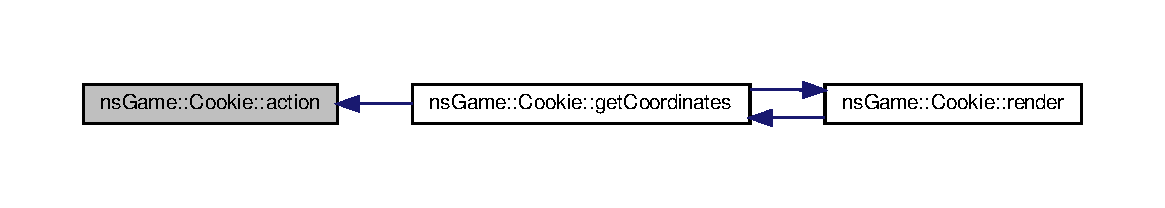
\includegraphics[width=350pt]{classns_game_1_1_cookie_a2cd4ee8c83b99191643d6e9ef2267b1a_icgraph}
\end{center}
\end{figure}
\mbox{\Hypertarget{classns_game_1_1_cookie_ab624101d018f74fb856bdfd7fd97c55e}\label{classns_game_1_1_cookie_ab624101d018f74fb856bdfd7fd97c55e}} 
\index{ns\+Game\+::\+Cookie@{ns\+Game\+::\+Cookie}!get\+Coordinates@{get\+Coordinates}}
\index{get\+Coordinates@{get\+Coordinates}!ns\+Game\+::\+Cookie@{ns\+Game\+::\+Cookie}}
\subsubsection{\texorpdfstring{get\+Coordinates()}{getCoordinates()}}
{\footnotesize\ttfamily ns\+Graphics\+::\+Vec2D ns\+Game\+::\+Cookie\+::get\+Coordinates (\begin{DoxyParamCaption}{ }\end{DoxyParamCaption})\hspace{0.3cm}{\ttfamily [inline]}}



This function is used to get the position on the screen/canvas/window, whatever you want to call it. 



Definition at line 32 of file cookie.\+h.

Here is the call graph for this function\+:\nopagebreak
\begin{figure}[H]
\begin{center}
\leavevmode
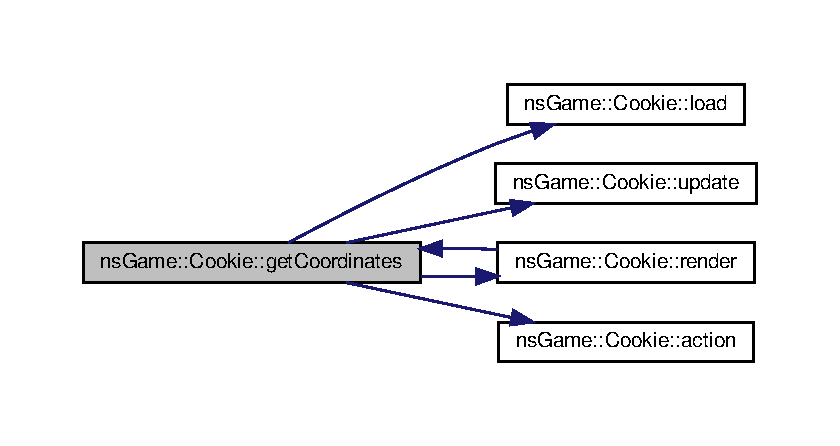
\includegraphics[width=350pt]{classns_game_1_1_cookie_ab624101d018f74fb856bdfd7fd97c55e_cgraph}
\end{center}
\end{figure}
Here is the caller graph for this function\+:\nopagebreak
\begin{figure}[H]
\begin{center}
\leavevmode
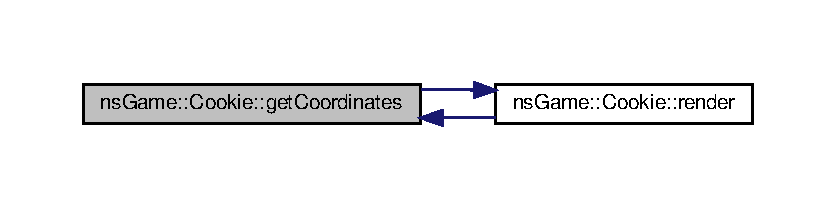
\includegraphics[width=350pt]{classns_game_1_1_cookie_ab624101d018f74fb856bdfd7fd97c55e_icgraph}
\end{center}
\end{figure}
\mbox{\Hypertarget{classns_game_1_1_cookie_ac5c28f610947708bc1f31b1e8a88ef42}\label{classns_game_1_1_cookie_ac5c28f610947708bc1f31b1e8a88ef42}} 
\index{ns\+Game\+::\+Cookie@{ns\+Game\+::\+Cookie}!get\+Type@{get\+Type}}
\index{get\+Type@{get\+Type}!ns\+Game\+::\+Cookie@{ns\+Game\+::\+Cookie}}
\subsubsection{\texorpdfstring{get\+Type()}{getType()}}
{\footnotesize\ttfamily \hyperlink{namespacens_game_a5f7db01e6447720e9a145f0b3c68a4d7}{Item\+Type} ns\+Game\+::\+Cookie\+::get\+Type (\begin{DoxyParamCaption}{ }\end{DoxyParamCaption})\hspace{0.3cm}{\ttfamily [inline]}, {\ttfamily [override]}, {\ttfamily [virtual]}}



Gets item type. 

\begin{DoxyReturn}{Returns}
Item\+Type.\+F\+O\+OD 
\end{DoxyReturn}


Reimplemented from \hyperlink{structns_game_1_1_item_a69156550e5083928cbb673ca2db671f5}{ns\+Game\+::\+Item}.



Definition at line 64 of file cookie.\+h.

\mbox{\Hypertarget{classns_game_1_1_cookie_a20769adf2b327f4bf519e851073b1891}\label{classns_game_1_1_cookie_a20769adf2b327f4bf519e851073b1891}} 
\index{ns\+Game\+::\+Cookie@{ns\+Game\+::\+Cookie}!load@{load}}
\index{load@{load}!ns\+Game\+::\+Cookie@{ns\+Game\+::\+Cookie}}
\subsubsection{\texorpdfstring{load()}{load()}}
{\footnotesize\ttfamily void ns\+Game\+::\+Cookie\+::load (\begin{DoxyParamCaption}{ }\end{DoxyParamCaption})\hspace{0.3cm}{\ttfamily [override]}, {\ttfamily [virtual]}}



Loads food. 



Implements \hyperlink{structns_game_1_1_item_a5887b6e9225ae8a276801225eca83808}{ns\+Game\+::\+Item}.



Definition at line 15 of file cookie.\+cpp.

Here is the caller graph for this function\+:\nopagebreak
\begin{figure}[H]
\begin{center}
\leavevmode
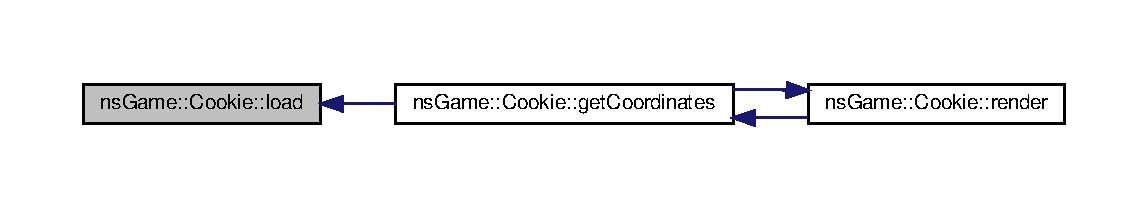
\includegraphics[width=350pt]{classns_game_1_1_cookie_a20769adf2b327f4bf519e851073b1891_icgraph}
\end{center}
\end{figure}
\mbox{\Hypertarget{classns_game_1_1_cookie_a7e321497bf9d9baa738d987e9c47dd5e}\label{classns_game_1_1_cookie_a7e321497bf9d9baa738d987e9c47dd5e}} 
\index{ns\+Game\+::\+Cookie@{ns\+Game\+::\+Cookie}!render@{render}}
\index{render@{render}!ns\+Game\+::\+Cookie@{ns\+Game\+::\+Cookie}}
\subsubsection{\texorpdfstring{render()}{render()}}
{\footnotesize\ttfamily void ns\+Game\+::\+Cookie\+::render (\begin{DoxyParamCaption}\item[{Min\+GL \&}]{window }\end{DoxyParamCaption})\hspace{0.3cm}{\ttfamily [override]}, {\ttfamily [virtual]}}



Renders resources. 



Implements \hyperlink{structns_game_1_1_item_a451b6491efc475c9ca47dcccdbbde707}{ns\+Game\+::\+Item}.



Definition at line 23 of file cookie.\+cpp.

Here is the call graph for this function\+:\nopagebreak
\begin{figure}[H]
\begin{center}
\leavevmode
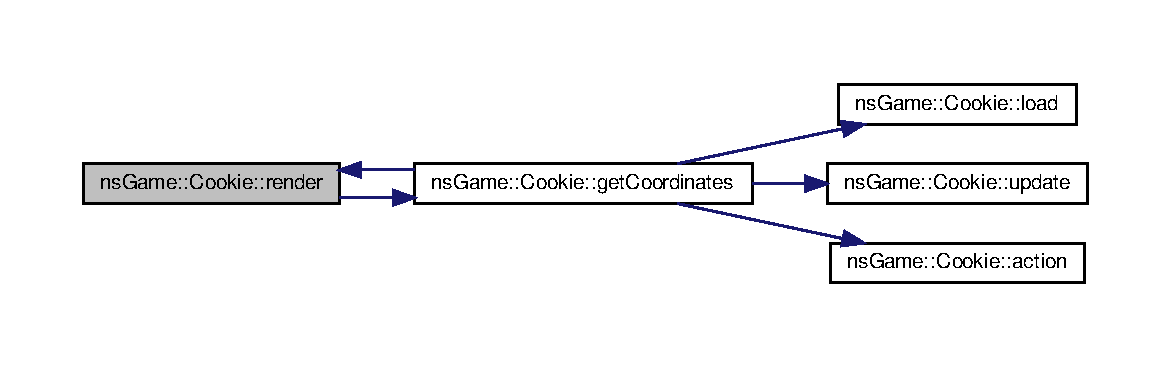
\includegraphics[width=350pt]{classns_game_1_1_cookie_a7e321497bf9d9baa738d987e9c47dd5e_cgraph}
\end{center}
\end{figure}
Here is the caller graph for this function\+:\nopagebreak
\begin{figure}[H]
\begin{center}
\leavevmode
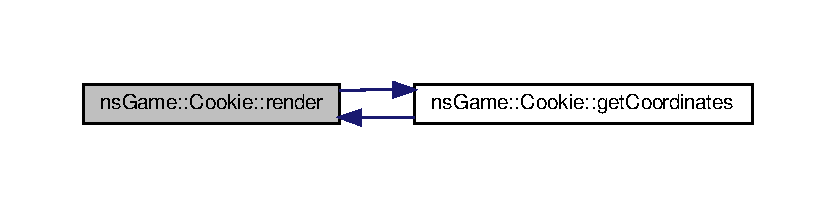
\includegraphics[width=350pt]{classns_game_1_1_cookie_a7e321497bf9d9baa738d987e9c47dd5e_icgraph}
\end{center}
\end{figure}
\mbox{\Hypertarget{classns_game_1_1_cookie_aaea5c3967effe908f2676a5ded17aa39}\label{classns_game_1_1_cookie_aaea5c3967effe908f2676a5ded17aa39}} 
\index{ns\+Game\+::\+Cookie@{ns\+Game\+::\+Cookie}!update@{update}}
\index{update@{update}!ns\+Game\+::\+Cookie@{ns\+Game\+::\+Cookie}}
\subsubsection{\texorpdfstring{update()}{update()}}
{\footnotesize\ttfamily void ns\+Game\+::\+Cookie\+::update (\begin{DoxyParamCaption}\item[{unsigned}]{delta }\end{DoxyParamCaption})\hspace{0.3cm}{\ttfamily [override]}, {\ttfamily [virtual]}}



Updates food. 



Implements \hyperlink{structns_game_1_1_item_a96c07d0f91eef0d77e91d1a7397091a1}{ns\+Game\+::\+Item}.



Definition at line 17 of file cookie.\+cpp.

Here is the caller graph for this function\+:\nopagebreak
\begin{figure}[H]
\begin{center}
\leavevmode
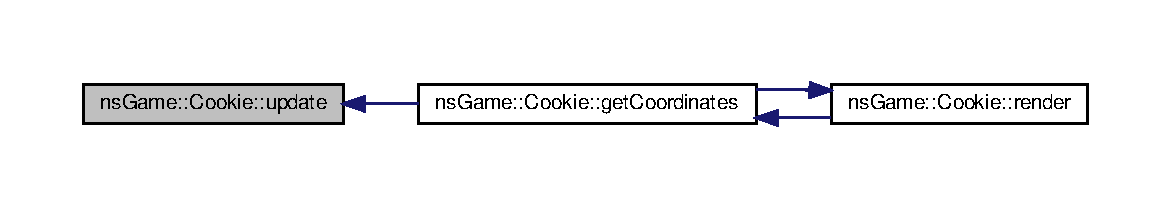
\includegraphics[width=350pt]{classns_game_1_1_cookie_aaea5c3967effe908f2676a5ded17aa39_icgraph}
\end{center}
\end{figure}


The documentation for this class was generated from the following files\+:\begin{DoxyCompactItemize}
\item 
Nos\+\_\+fichiers/\hyperlink{cookie_8h}{cookie.\+h}\item 
Nos\+\_\+fichiers/\hyperlink{cookie_8cpp}{cookie.\+cpp}\end{DoxyCompactItemize}

\hypertarget{classns_game_1_1_cooldowns}{}\section{ns\+Game\+:\+:Cooldowns Class Reference}
\label{classns_game_1_1_cooldowns}\index{ns\+Game\+::\+Cooldowns@{ns\+Game\+::\+Cooldowns}}


{\ttfamily \#include $<$cooldowns.\+h$>$}

\subsection*{Static Public Member Functions}
\begin{DoxyCompactItemize}
\item 
static void \hyperlink{classns_game_1_1_cooldowns_a70e8df0692a58a08b31b2b6c9578265e}{create\+Cooldown} (std\+::string id, unsigned delay)
\begin{DoxyCompactList}\small\item\em Saves a cooldown into the map. \end{DoxyCompactList}\item 
static void \hyperlink{classns_game_1_1_cooldowns_a35012d31be60c3743363d0487f2cead9}{update\+Cooldowns} (unsigned delta)
\begin{DoxyCompactList}\small\item\em Updates cooldowns according to frame delta. \end{DoxyCompactList}\item 
static bool \hyperlink{classns_game_1_1_cooldowns_a423a58fcbbf7688556c5706249365f12}{is\+Cooldown\+Over} (std\+::string id)
\begin{DoxyCompactList}\small\item\em Checks if a cooldown is over. \end{DoxyCompactList}\item 
static bool \hyperlink{classns_game_1_1_cooldowns_ace34dc5863d0cf6aa01120832b382cd2}{is\+Cooldown\+Over} (std\+::string id, bool has\+To\+Delete)
\begin{DoxyCompactList}\small\item\em Checks if a cooldown is over, and deletes it if has\+To\+Delete=true. \end{DoxyCompactList}\item 
static void \hyperlink{classns_game_1_1_cooldowns_a0db5b81efac93aacc0b12b2aa520620b}{set\+Cooldown\+Delay} (std\+::string id, unsigned delay)
\begin{DoxyCompactList}\small\item\em Sets a new delay for a cooldown that had been saved already. \end{DoxyCompactList}\item 
static void \hyperlink{classns_game_1_1_cooldowns_a820c7d29780f60b9f5ac5440e134de2e}{reset\+Cooldowns} ()
\begin{DoxyCompactList}\small\item\em Removes all cooldowns. \end{DoxyCompactList}\end{DoxyCompactItemize}


\subsection{Detailed Description}


Definition at line 18 of file cooldowns.\+h.



\subsection{Member Function Documentation}
\mbox{\Hypertarget{classns_game_1_1_cooldowns_a70e8df0692a58a08b31b2b6c9578265e}\label{classns_game_1_1_cooldowns_a70e8df0692a58a08b31b2b6c9578265e}} 
\index{ns\+Game\+::\+Cooldowns@{ns\+Game\+::\+Cooldowns}!create\+Cooldown@{create\+Cooldown}}
\index{create\+Cooldown@{create\+Cooldown}!ns\+Game\+::\+Cooldowns@{ns\+Game\+::\+Cooldowns}}
\subsubsection{\texorpdfstring{create\+Cooldown()}{createCooldown()}}
{\footnotesize\ttfamily void Cooldowns\+::create\+Cooldown (\begin{DoxyParamCaption}\item[{std\+::string}]{id,  }\item[{unsigned}]{delay }\end{DoxyParamCaption})\hspace{0.3cm}{\ttfamily [static]}}



Saves a cooldown into the map. 


\begin{DoxyParams}{Parameters}
{\em std\+::string} & id \\
\hline
{\em int} & delay \\
\hline
\end{DoxyParams}


Definition at line 14 of file cooldowns.\+cpp.

Here is the caller graph for this function\+:\nopagebreak
\begin{figure}[H]
\begin{center}
\leavevmode
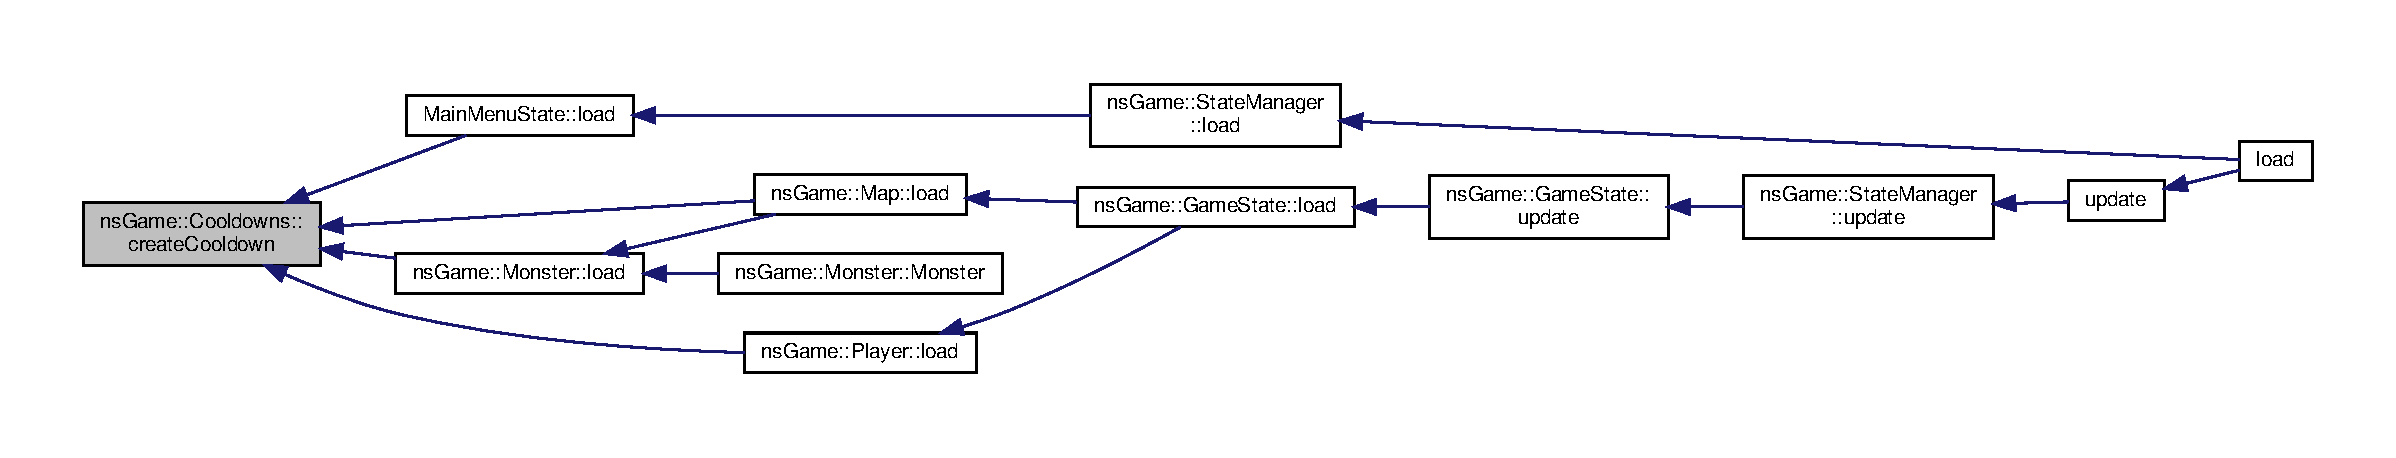
\includegraphics[width=350pt]{classns_game_1_1_cooldowns_a70e8df0692a58a08b31b2b6c9578265e_icgraph}
\end{center}
\end{figure}
\mbox{\Hypertarget{classns_game_1_1_cooldowns_a423a58fcbbf7688556c5706249365f12}\label{classns_game_1_1_cooldowns_a423a58fcbbf7688556c5706249365f12}} 
\index{ns\+Game\+::\+Cooldowns@{ns\+Game\+::\+Cooldowns}!is\+Cooldown\+Over@{is\+Cooldown\+Over}}
\index{is\+Cooldown\+Over@{is\+Cooldown\+Over}!ns\+Game\+::\+Cooldowns@{ns\+Game\+::\+Cooldowns}}
\subsubsection{\texorpdfstring{is\+Cooldown\+Over()}{isCooldownOver()}\hspace{0.1cm}{\footnotesize\ttfamily [1/2]}}
{\footnotesize\ttfamily bool Cooldowns\+::is\+Cooldown\+Over (\begin{DoxyParamCaption}\item[{std\+::string}]{id }\end{DoxyParamCaption})\hspace{0.3cm}{\ttfamily [static]}}



Checks if a cooldown is over. 


\begin{DoxyParams}{Parameters}
{\em std\+::string} & id \\
\hline
\end{DoxyParams}
\begin{DoxyReturn}{Returns}

\end{DoxyReturn}


Definition at line 23 of file cooldowns.\+cpp.

Here is the caller graph for this function\+:\nopagebreak
\begin{figure}[H]
\begin{center}
\leavevmode
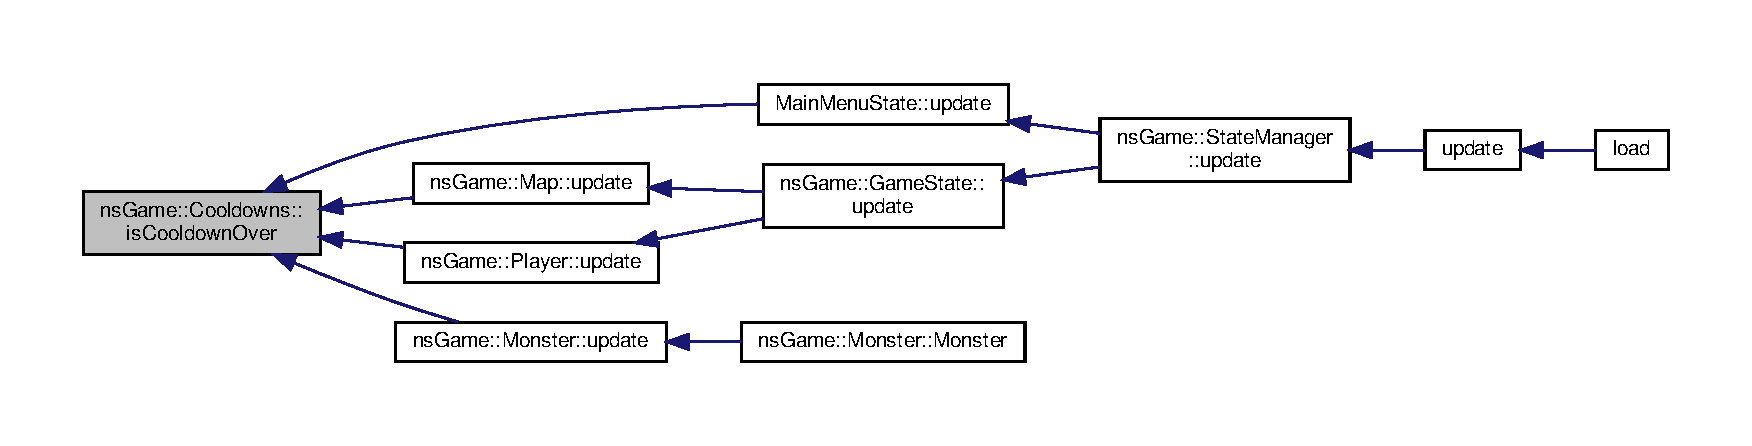
\includegraphics[width=350pt]{classns_game_1_1_cooldowns_a423a58fcbbf7688556c5706249365f12_icgraph}
\end{center}
\end{figure}
\mbox{\Hypertarget{classns_game_1_1_cooldowns_ace34dc5863d0cf6aa01120832b382cd2}\label{classns_game_1_1_cooldowns_ace34dc5863d0cf6aa01120832b382cd2}} 
\index{ns\+Game\+::\+Cooldowns@{ns\+Game\+::\+Cooldowns}!is\+Cooldown\+Over@{is\+Cooldown\+Over}}
\index{is\+Cooldown\+Over@{is\+Cooldown\+Over}!ns\+Game\+::\+Cooldowns@{ns\+Game\+::\+Cooldowns}}
\subsubsection{\texorpdfstring{is\+Cooldown\+Over()}{isCooldownOver()}\hspace{0.1cm}{\footnotesize\ttfamily [2/2]}}
{\footnotesize\ttfamily bool Cooldowns\+::is\+Cooldown\+Over (\begin{DoxyParamCaption}\item[{std\+::string}]{id,  }\item[{bool}]{has\+To\+Delete }\end{DoxyParamCaption})\hspace{0.3cm}{\ttfamily [static]}}



Checks if a cooldown is over, and deletes it if has\+To\+Delete=true. 


\begin{DoxyParams}{Parameters}
{\em std\+::string} & id \\
\hline
{\em bool} & has\+To\+Delete \\
\hline
\end{DoxyParams}
\begin{DoxyReturn}{Returns}

\end{DoxyReturn}


Definition at line 34 of file cooldowns.\+cpp.

\mbox{\Hypertarget{classns_game_1_1_cooldowns_a820c7d29780f60b9f5ac5440e134de2e}\label{classns_game_1_1_cooldowns_a820c7d29780f60b9f5ac5440e134de2e}} 
\index{ns\+Game\+::\+Cooldowns@{ns\+Game\+::\+Cooldowns}!reset\+Cooldowns@{reset\+Cooldowns}}
\index{reset\+Cooldowns@{reset\+Cooldowns}!ns\+Game\+::\+Cooldowns@{ns\+Game\+::\+Cooldowns}}
\subsubsection{\texorpdfstring{reset\+Cooldowns()}{resetCooldowns()}}
{\footnotesize\ttfamily void Cooldowns\+::reset\+Cooldowns (\begin{DoxyParamCaption}{ }\end{DoxyParamCaption})\hspace{0.3cm}{\ttfamily [static]}}



Removes all cooldowns. 



Definition at line 49 of file cooldowns.\+cpp.

\mbox{\Hypertarget{classns_game_1_1_cooldowns_a0db5b81efac93aacc0b12b2aa520620b}\label{classns_game_1_1_cooldowns_a0db5b81efac93aacc0b12b2aa520620b}} 
\index{ns\+Game\+::\+Cooldowns@{ns\+Game\+::\+Cooldowns}!set\+Cooldown\+Delay@{set\+Cooldown\+Delay}}
\index{set\+Cooldown\+Delay@{set\+Cooldown\+Delay}!ns\+Game\+::\+Cooldowns@{ns\+Game\+::\+Cooldowns}}
\subsubsection{\texorpdfstring{set\+Cooldown\+Delay()}{setCooldownDelay()}}
{\footnotesize\ttfamily void Cooldowns\+::set\+Cooldown\+Delay (\begin{DoxyParamCaption}\item[{std\+::string}]{id,  }\item[{unsigned}]{delay }\end{DoxyParamCaption})\hspace{0.3cm}{\ttfamily [static]}}



Sets a new delay for a cooldown that had been saved already. 


\begin{DoxyParams}{Parameters}
{\em std\+::string} & id \\
\hline
{\em unsigned} & delay \\
\hline
\end{DoxyParams}


Definition at line 45 of file cooldowns.\+cpp.

Here is the caller graph for this function\+:\nopagebreak
\begin{figure}[H]
\begin{center}
\leavevmode
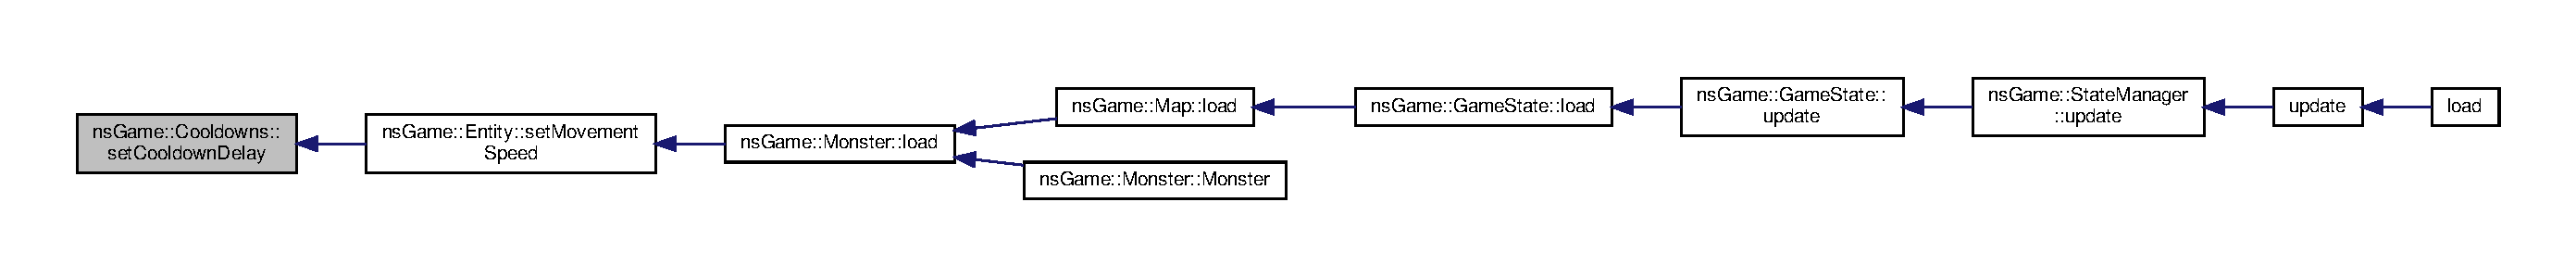
\includegraphics[width=350pt]{classns_game_1_1_cooldowns_a0db5b81efac93aacc0b12b2aa520620b_icgraph}
\end{center}
\end{figure}
\mbox{\Hypertarget{classns_game_1_1_cooldowns_a35012d31be60c3743363d0487f2cead9}\label{classns_game_1_1_cooldowns_a35012d31be60c3743363d0487f2cead9}} 
\index{ns\+Game\+::\+Cooldowns@{ns\+Game\+::\+Cooldowns}!update\+Cooldowns@{update\+Cooldowns}}
\index{update\+Cooldowns@{update\+Cooldowns}!ns\+Game\+::\+Cooldowns@{ns\+Game\+::\+Cooldowns}}
\subsubsection{\texorpdfstring{update\+Cooldowns()}{updateCooldowns()}}
{\footnotesize\ttfamily void Cooldowns\+::update\+Cooldowns (\begin{DoxyParamCaption}\item[{unsigned}]{delta }\end{DoxyParamCaption})\hspace{0.3cm}{\ttfamily [static]}}



Updates cooldowns according to frame delta. 


\begin{DoxyParams}{Parameters}
{\em unsigned} & delta \\
\hline
\end{DoxyParams}


Definition at line 18 of file cooldowns.\+cpp.



The documentation for this class was generated from the following files\+:\begin{DoxyCompactItemize}
\item 
Nos\+\_\+fichiers/\hyperlink{cooldowns_8h}{cooldowns.\+h}\item 
Nos\+\_\+fichiers/\hyperlink{cooldowns_8cpp}{cooldowns.\+cpp}\end{DoxyCompactItemize}

\hypertarget{class_credit_state}{}\section{Credit\+State Class Reference}
\label{class_credit_state}\index{Credit\+State@{Credit\+State}}


Defines the credits.  




Inheritance diagram for Credit\+State\+:\nopagebreak
\begin{figure}[H]
\begin{center}
\leavevmode
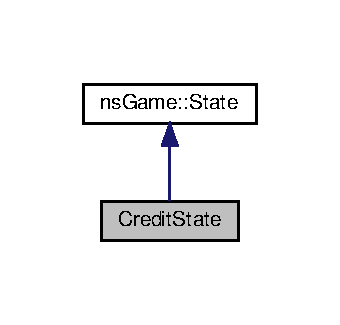
\includegraphics[width=163pt]{class_credit_state__inherit__graph}
\end{center}
\end{figure}


Collaboration diagram for Credit\+State\+:\nopagebreak
\begin{figure}[H]
\begin{center}
\leavevmode
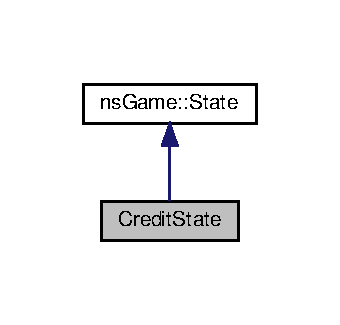
\includegraphics[width=163pt]{class_credit_state__coll__graph}
\end{center}
\end{figure}
\subsection*{Public Member Functions}
\begin{DoxyCompactItemize}
\item 
void \hyperlink{class_credit_state_a32ec8ae5c12ee636cfd2b949b8e980e1}{load} () override
\begin{DoxyCompactList}\small\item\em Loads State resources. \end{DoxyCompactList}\item 
void \hyperlink{class_credit_state_a52a92d650fce22fa08b37359c3a5aa64}{update} (Min\+GL \&window, unsigned delta) override
\begin{DoxyCompactList}\small\item\em Updates state. \end{DoxyCompactList}\item 
void \hyperlink{class_credit_state_aa4ba316fca29d0e79ee70891e373a060}{render} (Min\+GL \&window) override
\begin{DoxyCompactList}\small\item\em Renders resources. \end{DoxyCompactList}\end{DoxyCompactItemize}
\subsection*{Public Attributes}
\begin{DoxyCompactItemize}
\item 
ns\+Gui\+::\+Sprite \hyperlink{class_credit_state_a10ae436f8c1ca5d87cc960ada3cadb18}{sprite} = ns\+Gui\+::\+Sprite(\hyperlink{definitions_8h_a793644bd88146828177a2a4f57e3bf01}{R\+E\+S\+\_\+\+P\+A\+TH} + \char`\"{}/gui/credits.\+i2s\char`\"{}, ns\+Graphics\+::\+Vec2D(0, 0))
\item 
ns\+Transition\+::\+Transition\+Engine \hyperlink{class_credit_state_a12c76114d83f1788b356c0cbbc74bcaf}{transition\+Engine}
\item 
ns\+Audio\+::\+Audio\+Engine \hyperlink{class_credit_state_a8dd128ec1e8d3b8da0da5bd0be38c96d}{audio}
\end{DoxyCompactItemize}


\subsection{Detailed Description}
Defines the credits. 

\begin{DoxyAuthor}{Authors}
Thomas Cardon, Alexandre Arniaud 
\end{DoxyAuthor}


Definition at line 19 of file credit\+State.\+cpp.



\subsection{Member Function Documentation}
\mbox{\Hypertarget{class_credit_state_a32ec8ae5c12ee636cfd2b949b8e980e1}\label{class_credit_state_a32ec8ae5c12ee636cfd2b949b8e980e1}} 
\index{Credit\+State@{Credit\+State}!load@{load}}
\index{load@{load}!Credit\+State@{Credit\+State}}
\subsubsection{\texorpdfstring{load()}{load()}}
{\footnotesize\ttfamily void Credit\+State\+::load (\begin{DoxyParamCaption}{ }\end{DoxyParamCaption})\hspace{0.3cm}{\ttfamily [inline]}, {\ttfamily [override]}, {\ttfamily [virtual]}}



Loads State resources. 



Reimplemented from \hyperlink{structns_game_1_1_state_a8644de505f7a84933f6d6e6651205791}{ns\+Game\+::\+State}.



Definition at line 30 of file credit\+State.\+cpp.

Here is the caller graph for this function\+:\nopagebreak
\begin{figure}[H]
\begin{center}
\leavevmode
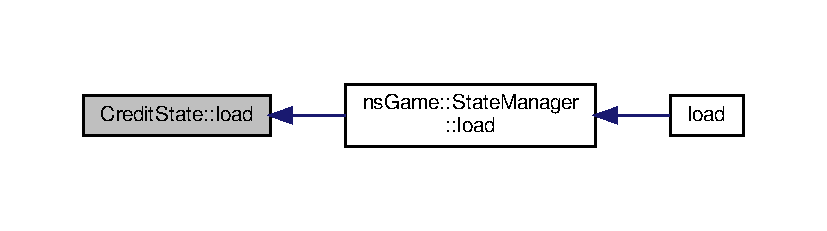
\includegraphics[width=350pt]{class_credit_state_a32ec8ae5c12ee636cfd2b949b8e980e1_icgraph}
\end{center}
\end{figure}
\mbox{\Hypertarget{class_credit_state_aa4ba316fca29d0e79ee70891e373a060}\label{class_credit_state_aa4ba316fca29d0e79ee70891e373a060}} 
\index{Credit\+State@{Credit\+State}!render@{render}}
\index{render@{render}!Credit\+State@{Credit\+State}}
\subsubsection{\texorpdfstring{render()}{render()}}
{\footnotesize\ttfamily void Credit\+State\+::render (\begin{DoxyParamCaption}\item[{Min\+GL \&}]{window }\end{DoxyParamCaption})\hspace{0.3cm}{\ttfamily [inline]}, {\ttfamily [override]}, {\ttfamily [virtual]}}



Renders resources. 



Reimplemented from \hyperlink{structns_game_1_1_state_a214f8ee52de4b318f1ed3861a578ce67}{ns\+Game\+::\+State}.



Definition at line 49 of file credit\+State.\+cpp.

Here is the caller graph for this function\+:\nopagebreak
\begin{figure}[H]
\begin{center}
\leavevmode
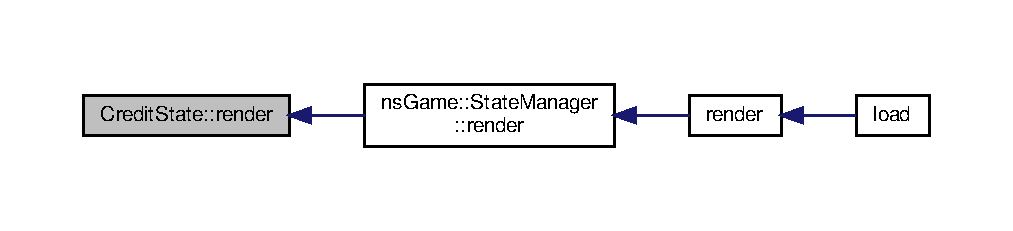
\includegraphics[width=350pt]{class_credit_state_aa4ba316fca29d0e79ee70891e373a060_icgraph}
\end{center}
\end{figure}
\mbox{\Hypertarget{class_credit_state_a52a92d650fce22fa08b37359c3a5aa64}\label{class_credit_state_a52a92d650fce22fa08b37359c3a5aa64}} 
\index{Credit\+State@{Credit\+State}!update@{update}}
\index{update@{update}!Credit\+State@{Credit\+State}}
\subsubsection{\texorpdfstring{update()}{update()}}
{\footnotesize\ttfamily void Credit\+State\+::update (\begin{DoxyParamCaption}\item[{Min\+GL \&}]{window,  }\item[{unsigned}]{delta }\end{DoxyParamCaption})\hspace{0.3cm}{\ttfamily [inline]}, {\ttfamily [override]}, {\ttfamily [virtual]}}



Updates state. 



Reimplemented from \hyperlink{structns_game_1_1_state_ae809e89ac9df4a43ab90d5d5932e2bc7}{ns\+Game\+::\+State}.



Definition at line 39 of file credit\+State.\+cpp.

Here is the caller graph for this function\+:\nopagebreak
\begin{figure}[H]
\begin{center}
\leavevmode
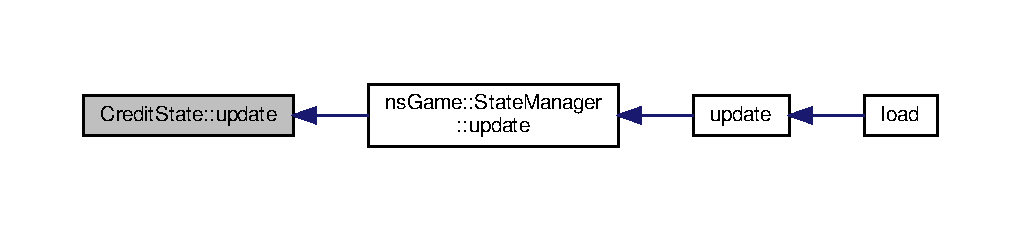
\includegraphics[width=350pt]{class_credit_state_a52a92d650fce22fa08b37359c3a5aa64_icgraph}
\end{center}
\end{figure}


\subsection{Member Data Documentation}
\mbox{\Hypertarget{class_credit_state_a8dd128ec1e8d3b8da0da5bd0be38c96d}\label{class_credit_state_a8dd128ec1e8d3b8da0da5bd0be38c96d}} 
\index{Credit\+State@{Credit\+State}!audio@{audio}}
\index{audio@{audio}!Credit\+State@{Credit\+State}}
\subsubsection{\texorpdfstring{audio}{audio}}
{\footnotesize\ttfamily ns\+Audio\+::\+Audio\+Engine Credit\+State\+::audio}



Definition at line 28 of file credit\+State.\+cpp.

\mbox{\Hypertarget{class_credit_state_a10ae436f8c1ca5d87cc960ada3cadb18}\label{class_credit_state_a10ae436f8c1ca5d87cc960ada3cadb18}} 
\index{Credit\+State@{Credit\+State}!sprite@{sprite}}
\index{sprite@{sprite}!Credit\+State@{Credit\+State}}
\subsubsection{\texorpdfstring{sprite}{sprite}}
{\footnotesize\ttfamily ns\+Gui\+::\+Sprite Credit\+State\+::sprite = ns\+Gui\+::\+Sprite(\hyperlink{definitions_8h_a793644bd88146828177a2a4f57e3bf01}{R\+E\+S\+\_\+\+P\+A\+TH} + \char`\"{}/gui/credits.\+i2s\char`\"{}, ns\+Graphics\+::\+Vec2D(0, 0))}



Definition at line 26 of file credit\+State.\+cpp.

\mbox{\Hypertarget{class_credit_state_a12c76114d83f1788b356c0cbbc74bcaf}\label{class_credit_state_a12c76114d83f1788b356c0cbbc74bcaf}} 
\index{Credit\+State@{Credit\+State}!transition\+Engine@{transition\+Engine}}
\index{transition\+Engine@{transition\+Engine}!Credit\+State@{Credit\+State}}
\subsubsection{\texorpdfstring{transition\+Engine}{transitionEngine}}
{\footnotesize\ttfamily ns\+Transition\+::\+Transition\+Engine Credit\+State\+::transition\+Engine}



Definition at line 27 of file credit\+State.\+cpp.



The documentation for this class was generated from the following file\+:\begin{DoxyCompactItemize}
\item 
Nos\+\_\+fichiers/\hyperlink{credit_state_8cpp}{credit\+State.\+cpp}\end{DoxyCompactItemize}

\hypertarget{structns_game_1_1_entity}{}\section{ns\+Game\+:\+:Entity Class Reference}
\label{structns_game_1_1_entity}\index{ns\+Game\+::\+Entity@{ns\+Game\+::\+Entity}}


Defines the \hyperlink{structns_game_1_1_entity}{Entity} class.  




{\ttfamily \#include $<$entity.\+h$>$}



Inheritance diagram for ns\+Game\+:\+:Entity\+:\nopagebreak
\begin{figure}[H]
\begin{center}
\leavevmode
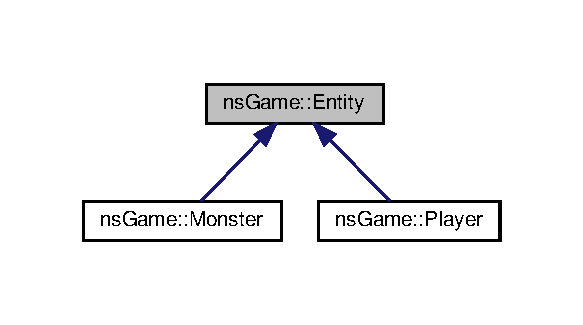
\includegraphics[width=280pt]{structns_game_1_1_entity__inherit__graph}
\end{center}
\end{figure}
\subsection*{Public Member Functions}
\begin{DoxyCompactItemize}
\item 
void \hyperlink{structns_game_1_1_entity_ae0aa595447b5f3d2c0b80fb99305c56e}{load} ()
\begin{DoxyCompactList}\small\item\em load \end{DoxyCompactList}\item 
void \hyperlink{structns_game_1_1_entity_af1da5da20798e01469c4a438d0b4174c}{update} (unsigned delta, \hyperlink{type_8h_a64a592133575ccebb1b36453acbec02b}{C\+Mat} \&mat)
\begin{DoxyCompactList}\small\item\em update \end{DoxyCompactList}\item 
void \hyperlink{structns_game_1_1_entity_a4663cc85381acc9aaac120a85b6f24d0}{render} (Min\+GL \&window)
\begin{DoxyCompactList}\small\item\em render \end{DoxyCompactList}\item 
std\+::string \hyperlink{structns_game_1_1_entity_aa0057e4e5b73cc0187602c3180347a3a}{id} ()
\begin{DoxyCompactList}\small\item\em Returns an entity ID, allows the game to set cooldowns or whatever associated with its ID. \end{DoxyCompactList}\item 
ns\+Graphics\+::\+Vec2D \hyperlink{structns_game_1_1_entity_a727ed96ea0a27b7232e701ed0ba6d3a4}{get\+Coordinates} ()
\begin{DoxyCompactList}\small\item\em This function is used to get the position on the screen/canvas/window, whatever you want to call it. \end{DoxyCompactList}\item 
ns\+Graphics\+::\+Vec2D \hyperlink{structns_game_1_1_entity_ab7fc1631346d2c643161d229dd653edd}{get\+Position} ()
\begin{DoxyCompactList}\small\item\em Gets the coordinates compared to the map. \end{DoxyCompactList}\item 
void \hyperlink{structns_game_1_1_entity_ac09f45ca50c9fef57a50c4414fc7e20d}{spawn} ()
\begin{DoxyCompactList}\small\item\em Teleports the entity at its spawn. \end{DoxyCompactList}\item 
double \hyperlink{structns_game_1_1_entity_a03b934337b3c013abcccf3dfea6396d1}{get\+Movement\+Speed} ()
\begin{DoxyCompactList}\small\item\em Gets the movement speed. \end{DoxyCompactList}\item 
void \hyperlink{structns_game_1_1_entity_a0254c30b6223caa723303266ad04e4cd}{set\+Movement\+Speed} (double speed)
\begin{DoxyCompactList}\small\item\em Sets the movement speed. \end{DoxyCompactList}\item 
bool \hyperlink{structns_game_1_1_entity_a5dd00624fa76be09de80a6d2a982ea09}{in\+Collision} (\hyperlink{type_8h_a64a592133575ccebb1b36453acbec02b}{C\+Mat} map, unsigned x, unsigned y)
\begin{DoxyCompactList}\small\item\em Checks if entity would be in collision with a structure (walls...) $\vert$ O\+V\+E\+R\+R\+I\+DE IF N\+E\+E\+D\+ED (Flying monsters?) \end{DoxyCompactList}\item 
bool \hyperlink{structns_game_1_1_entity_ab5e14a11c0e89dce65f14366989a03b9}{can\+Be\+Hit\+By} (\hyperlink{structns_game_1_1_entity}{Entity} $\ast$entity)
\begin{DoxyCompactList}\small\item\em Checks if entity can be hit by another entity. \end{DoxyCompactList}\item 
void \hyperlink{structns_game_1_1_entity_a7a39068f9b48d1ec3fc5ef881e142b55}{damage} ()
\begin{DoxyCompactList}\small\item\em Damages entity. \end{DoxyCompactList}\item 
void \hyperlink{structns_game_1_1_entity_a522648b330daab91b49f78f0737a943f}{kill} ()
\item 
void \hyperlink{structns_game_1_1_entity_a0fbe0a80400a03319fbe3bd50919535c}{add\+Effect} (\hyperlink{namespacens_game_afea521dd2ba8e97be9549ce9936f4522}{Effect\+Type} type, unsigned delay)
\begin{DoxyCompactList}\small\item\em Adds an effect to the entity for x milliseconds. \end{DoxyCompactList}\item 
void \hyperlink{structns_game_1_1_entity_accc47c70658884bd70938642fc1cc431}{remove\+Effect} (\hyperlink{namespacens_game_afea521dd2ba8e97be9549ce9936f4522}{Effect\+Type} type)
\begin{DoxyCompactList}\small\item\em Removes an effect from the entity. \end{DoxyCompactList}\item 
bool \hyperlink{structns_game_1_1_entity_af5bf634702f96ed5daac8130a3dee4f0}{has\+Effect} (\hyperlink{namespacens_game_afea521dd2ba8e97be9549ce9936f4522}{Effect\+Type} type)
\begin{DoxyCompactList}\small\item\em Says if entity has effect. \end{DoxyCompactList}\item 
unsigned \hyperlink{structns_game_1_1_entity_a0c574fba3e12b9bb976d72953626e550}{\+\_\+get\+Delay} ()
\begin{DoxyCompactList}\small\item\em Prevents entity to move for X milliseconds. \end{DoxyCompactList}\end{DoxyCompactItemize}
\subsection*{Public Attributes}
\begin{DoxyCompactItemize}
\item 
bool \hyperlink{structns_game_1_1_entity_a3b26c2bf34732b4621932ab7d50421e9}{is\+Allowed\+To\+Move} = true
\begin{DoxyCompactList}\small\item\em Prevents entity to move. \end{DoxyCompactList}\item 
bool \hyperlink{structns_game_1_1_entity_aaf71fbc10979dcc5b5af55fcb6e44216}{slain} = false
\begin{DoxyCompactList}\small\item\em Says if entity has been killed. \end{DoxyCompactList}\item 
ns\+Graphics\+::\+Vec2D \hyperlink{structns_game_1_1_entity_a1ad359bb31e86c4971fd96b080ed43c4}{pos}
\begin{DoxyCompactList}\small\item\em \hyperlink{structns_game_1_1_entity}{Entity} position. \end{DoxyCompactList}\end{DoxyCompactItemize}
\subsection*{Protected Attributes}
\begin{DoxyCompactItemize}
\item 
double \hyperlink{structns_game_1_1_entity_a2b5d83f01bdc1d58673b3fae9afe704e}{movement\+Speed} = 1.\+0
\begin{DoxyCompactList}\small\item\em Movement Speed. \end{DoxyCompactList}\end{DoxyCompactItemize}


\subsection{Detailed Description}
Defines the \hyperlink{structns_game_1_1_entity}{Entity} class. 

\begin{DoxyAuthor}{Author}
Thomas Cardon 
\end{DoxyAuthor}


Definition at line 27 of file entity.\+h.



\subsection{Member Function Documentation}
\mbox{\Hypertarget{structns_game_1_1_entity_a0c574fba3e12b9bb976d72953626e550}\label{structns_game_1_1_entity_a0c574fba3e12b9bb976d72953626e550}} 
\index{ns\+Game\+::\+Entity@{ns\+Game\+::\+Entity}!\+\_\+get\+Delay@{\+\_\+get\+Delay}}
\index{\+\_\+get\+Delay@{\+\_\+get\+Delay}!ns\+Game\+::\+Entity@{ns\+Game\+::\+Entity}}
\subsubsection{\texorpdfstring{\+\_\+get\+Delay()}{\_getDelay()}}
{\footnotesize\ttfamily unsigned ns\+Game\+::\+Entity\+::\+\_\+get\+Delay (\begin{DoxyParamCaption}{ }\end{DoxyParamCaption})\hspace{0.3cm}{\ttfamily [inline]}}



Prevents entity to move for X milliseconds. 



Definition at line 152 of file entity.\+h.

Here is the caller graph for this function\+:\nopagebreak
\begin{figure}[H]
\begin{center}
\leavevmode
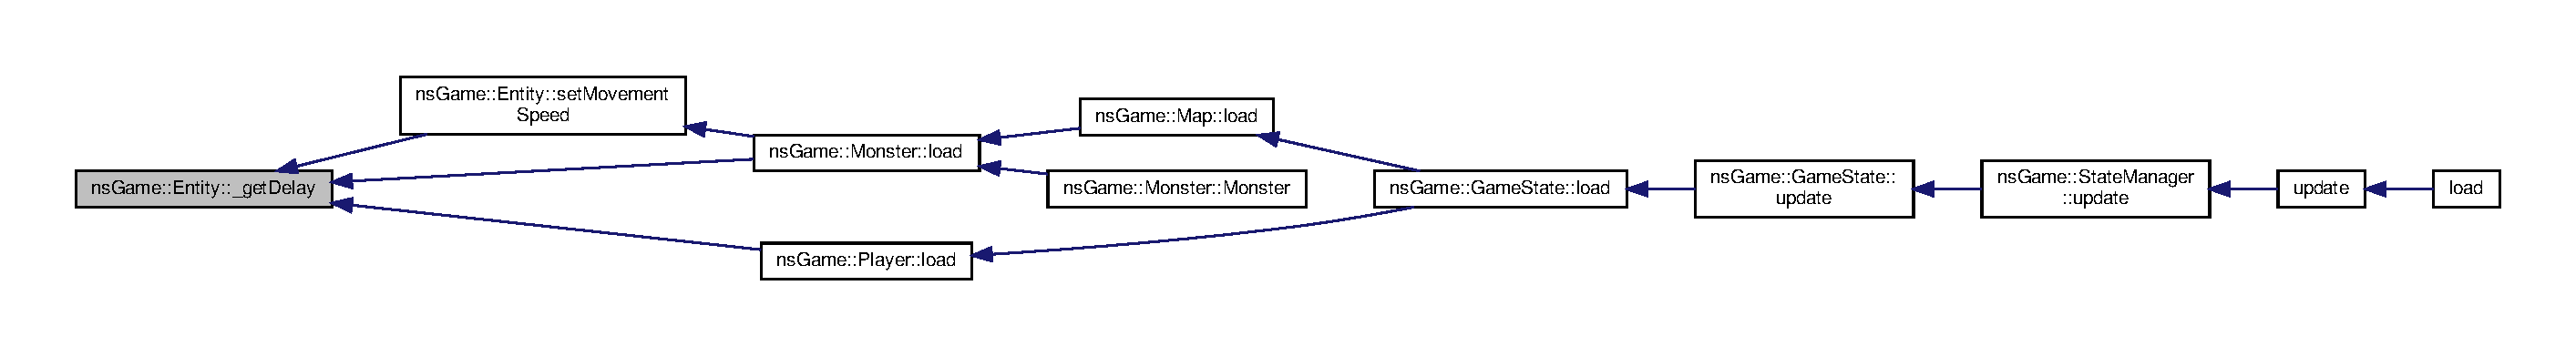
\includegraphics[width=350pt]{structns_game_1_1_entity_a0c574fba3e12b9bb976d72953626e550_icgraph}
\end{center}
\end{figure}
\mbox{\Hypertarget{structns_game_1_1_entity_a0fbe0a80400a03319fbe3bd50919535c}\label{structns_game_1_1_entity_a0fbe0a80400a03319fbe3bd50919535c}} 
\index{ns\+Game\+::\+Entity@{ns\+Game\+::\+Entity}!add\+Effect@{add\+Effect}}
\index{add\+Effect@{add\+Effect}!ns\+Game\+::\+Entity@{ns\+Game\+::\+Entity}}
\subsubsection{\texorpdfstring{add\+Effect()}{addEffect()}}
{\footnotesize\ttfamily void Entity\+::add\+Effect (\begin{DoxyParamCaption}\item[{\hyperlink{namespacens_game_afea521dd2ba8e97be9549ce9936f4522}{Effect\+Type}}]{type,  }\item[{unsigned}]{delay }\end{DoxyParamCaption})}



Adds an effect to the entity for x milliseconds. 


\begin{DoxyParams}{Parameters}
{\em Effect\+Type} & -\/ Effect ID \\
\hline
{\em unsigned} & delay \\
\hline
\end{DoxyParams}


Definition at line 103 of file entity.\+cpp.

Here is the caller graph for this function\+:\nopagebreak
\begin{figure}[H]
\begin{center}
\leavevmode
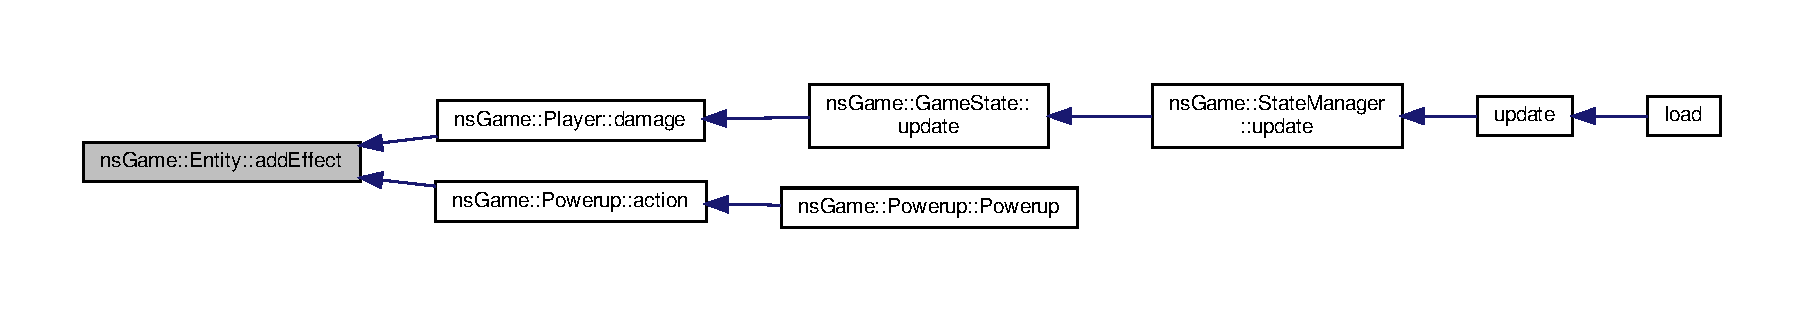
\includegraphics[width=350pt]{structns_game_1_1_entity_a0fbe0a80400a03319fbe3bd50919535c_icgraph}
\end{center}
\end{figure}
\mbox{\Hypertarget{structns_game_1_1_entity_ab5e14a11c0e89dce65f14366989a03b9}\label{structns_game_1_1_entity_ab5e14a11c0e89dce65f14366989a03b9}} 
\index{ns\+Game\+::\+Entity@{ns\+Game\+::\+Entity}!can\+Be\+Hit\+By@{can\+Be\+Hit\+By}}
\index{can\+Be\+Hit\+By@{can\+Be\+Hit\+By}!ns\+Game\+::\+Entity@{ns\+Game\+::\+Entity}}
\subsubsection{\texorpdfstring{can\+Be\+Hit\+By()}{canBeHitBy()}}
{\footnotesize\ttfamily bool ns\+Game\+::\+Entity\+::can\+Be\+Hit\+By (\begin{DoxyParamCaption}\item[{\hyperlink{structns_game_1_1_entity}{Entity} $\ast$}]{entity }\end{DoxyParamCaption})}



Checks if entity can be hit by another entity. 



Definition at line 78 of file entity.\+cpp.

Here is the call graph for this function\+:\nopagebreak
\begin{figure}[H]
\begin{center}
\leavevmode
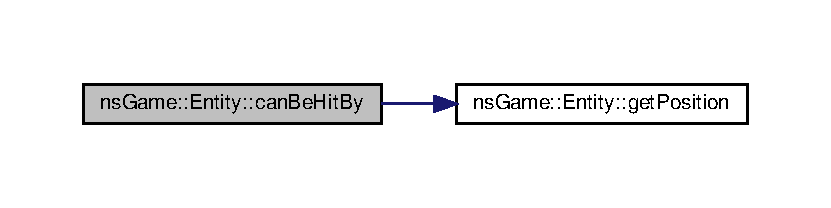
\includegraphics[width=350pt]{structns_game_1_1_entity_ab5e14a11c0e89dce65f14366989a03b9_cgraph}
\end{center}
\end{figure}
Here is the caller graph for this function\+:\nopagebreak
\begin{figure}[H]
\begin{center}
\leavevmode
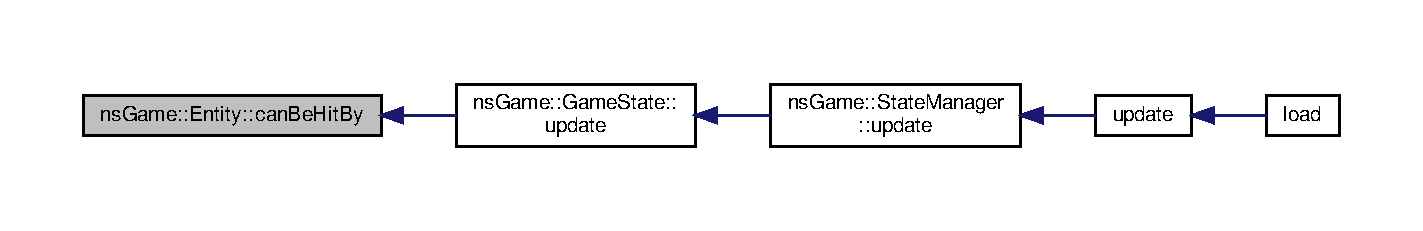
\includegraphics[width=350pt]{structns_game_1_1_entity_ab5e14a11c0e89dce65f14366989a03b9_icgraph}
\end{center}
\end{figure}
\mbox{\Hypertarget{structns_game_1_1_entity_a7a39068f9b48d1ec3fc5ef881e142b55}\label{structns_game_1_1_entity_a7a39068f9b48d1ec3fc5ef881e142b55}} 
\index{ns\+Game\+::\+Entity@{ns\+Game\+::\+Entity}!damage@{damage}}
\index{damage@{damage}!ns\+Game\+::\+Entity@{ns\+Game\+::\+Entity}}
\subsubsection{\texorpdfstring{damage()}{damage()}}
{\footnotesize\ttfamily void ns\+Game\+::\+Entity\+::damage (\begin{DoxyParamCaption}{ }\end{DoxyParamCaption})}



Damages entity. 

Kills entity. \mbox{\Hypertarget{structns_game_1_1_entity_a727ed96ea0a27b7232e701ed0ba6d3a4}\label{structns_game_1_1_entity_a727ed96ea0a27b7232e701ed0ba6d3a4}} 
\index{ns\+Game\+::\+Entity@{ns\+Game\+::\+Entity}!get\+Coordinates@{get\+Coordinates}}
\index{get\+Coordinates@{get\+Coordinates}!ns\+Game\+::\+Entity@{ns\+Game\+::\+Entity}}
\subsubsection{\texorpdfstring{get\+Coordinates()}{getCoordinates()}}
{\footnotesize\ttfamily ns\+Graphics\+::\+Vec2D ns\+Game\+::\+Entity\+::get\+Coordinates (\begin{DoxyParamCaption}{ }\end{DoxyParamCaption})}



This function is used to get the position on the screen/canvas/window, whatever you want to call it. 



Definition at line 54 of file entity.\+cpp.

Here is the call graph for this function\+:\nopagebreak
\begin{figure}[H]
\begin{center}
\leavevmode
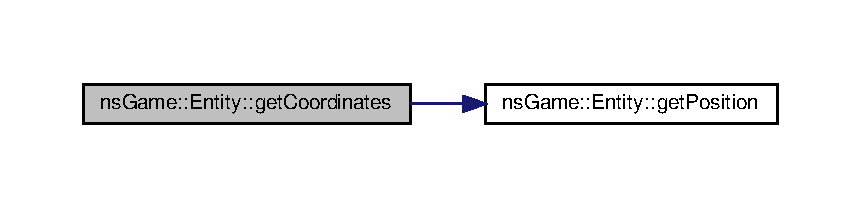
\includegraphics[width=350pt]{structns_game_1_1_entity_a727ed96ea0a27b7232e701ed0ba6d3a4_cgraph}
\end{center}
\end{figure}
Here is the caller graph for this function\+:\nopagebreak
\begin{figure}[H]
\begin{center}
\leavevmode
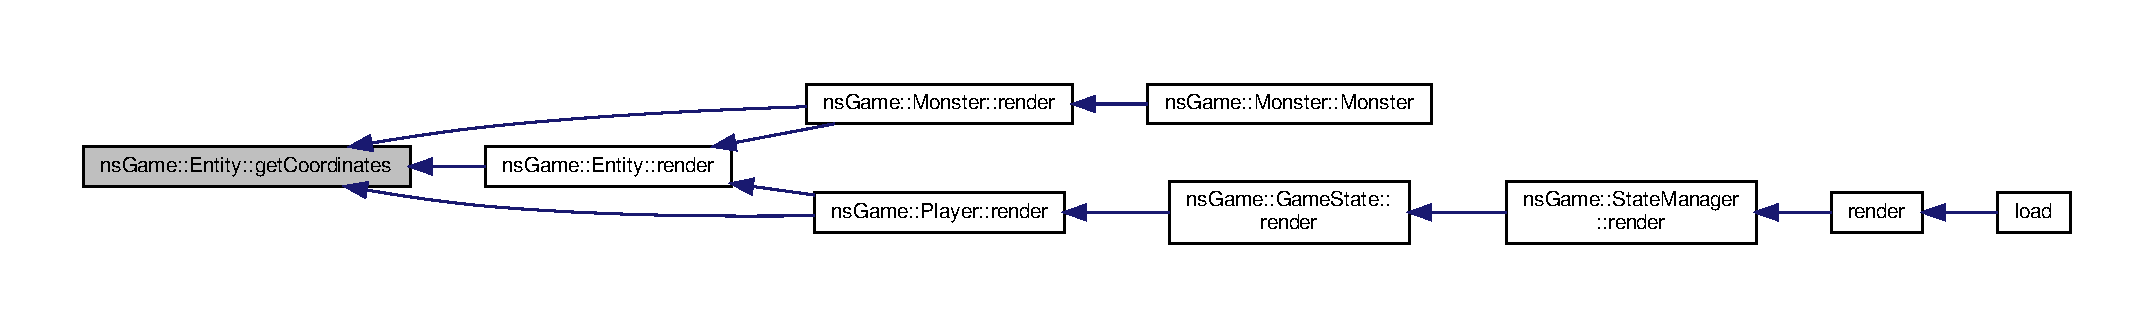
\includegraphics[width=350pt]{structns_game_1_1_entity_a727ed96ea0a27b7232e701ed0ba6d3a4_icgraph}
\end{center}
\end{figure}
\mbox{\Hypertarget{structns_game_1_1_entity_a03b934337b3c013abcccf3dfea6396d1}\label{structns_game_1_1_entity_a03b934337b3c013abcccf3dfea6396d1}} 
\index{ns\+Game\+::\+Entity@{ns\+Game\+::\+Entity}!get\+Movement\+Speed@{get\+Movement\+Speed}}
\index{get\+Movement\+Speed@{get\+Movement\+Speed}!ns\+Game\+::\+Entity@{ns\+Game\+::\+Entity}}
\subsubsection{\texorpdfstring{get\+Movement\+Speed()}{getMovementSpeed()}}
{\footnotesize\ttfamily bool ns\+Game\+::\+Entity\+::get\+Movement\+Speed (\begin{DoxyParamCaption}{ }\end{DoxyParamCaption})}



Gets the movement speed. 



Definition at line 90 of file entity.\+cpp.

\mbox{\Hypertarget{structns_game_1_1_entity_ab7fc1631346d2c643161d229dd653edd}\label{structns_game_1_1_entity_ab7fc1631346d2c643161d229dd653edd}} 
\index{ns\+Game\+::\+Entity@{ns\+Game\+::\+Entity}!get\+Position@{get\+Position}}
\index{get\+Position@{get\+Position}!ns\+Game\+::\+Entity@{ns\+Game\+::\+Entity}}
\subsubsection{\texorpdfstring{get\+Position()}{getPosition()}}
{\footnotesize\ttfamily ns\+Graphics\+::\+Vec2D ns\+Game\+::\+Entity\+::get\+Position (\begin{DoxyParamCaption}{ }\end{DoxyParamCaption})}



Gets the coordinates compared to the map. 



Definition at line 61 of file entity.\+cpp.

Here is the caller graph for this function\+:\nopagebreak
\begin{figure}[H]
\begin{center}
\leavevmode
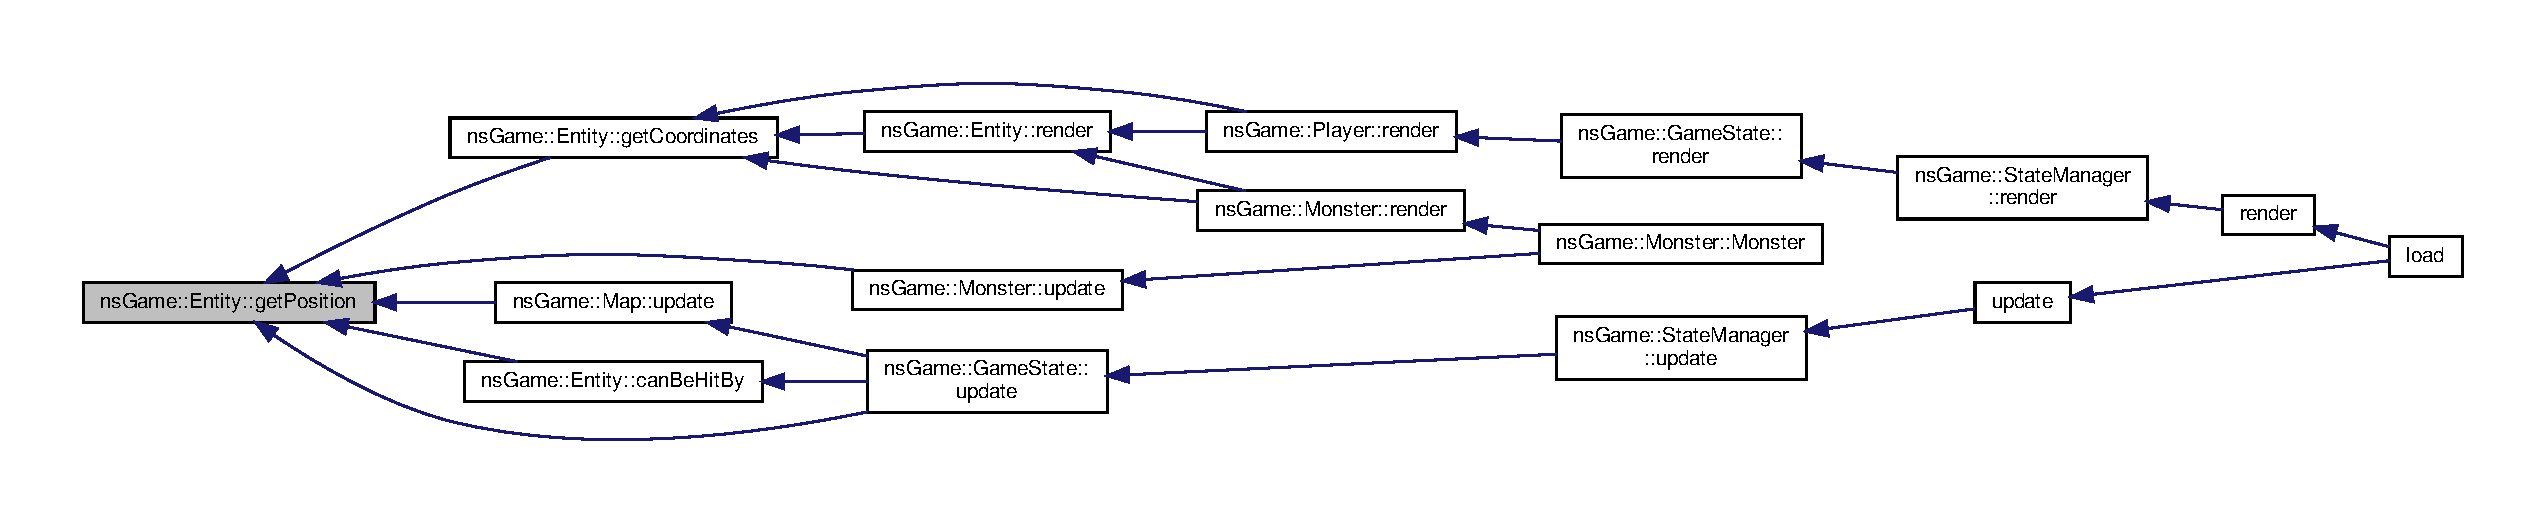
\includegraphics[width=350pt]{structns_game_1_1_entity_ab7fc1631346d2c643161d229dd653edd_icgraph}
\end{center}
\end{figure}
\mbox{\Hypertarget{structns_game_1_1_entity_af5bf634702f96ed5daac8130a3dee4f0}\label{structns_game_1_1_entity_af5bf634702f96ed5daac8130a3dee4f0}} 
\index{ns\+Game\+::\+Entity@{ns\+Game\+::\+Entity}!has\+Effect@{has\+Effect}}
\index{has\+Effect@{has\+Effect}!ns\+Game\+::\+Entity@{ns\+Game\+::\+Entity}}
\subsubsection{\texorpdfstring{has\+Effect()}{hasEffect()}}
{\footnotesize\ttfamily bool Entity\+::has\+Effect (\begin{DoxyParamCaption}\item[{\hyperlink{namespacens_game_afea521dd2ba8e97be9549ce9936f4522}{Effect\+Type}}]{type }\end{DoxyParamCaption})}



Says if entity has effect. 


\begin{DoxyParams}{Parameters}
{\em Effect\+Type} & type \\
\hline
\end{DoxyParams}
\begin{DoxyReturn}{Returns}
true if effect is present 
\end{DoxyReturn}


Definition at line 111 of file entity.\+cpp.

Here is the caller graph for this function\+:\nopagebreak
\begin{figure}[H]
\begin{center}
\leavevmode
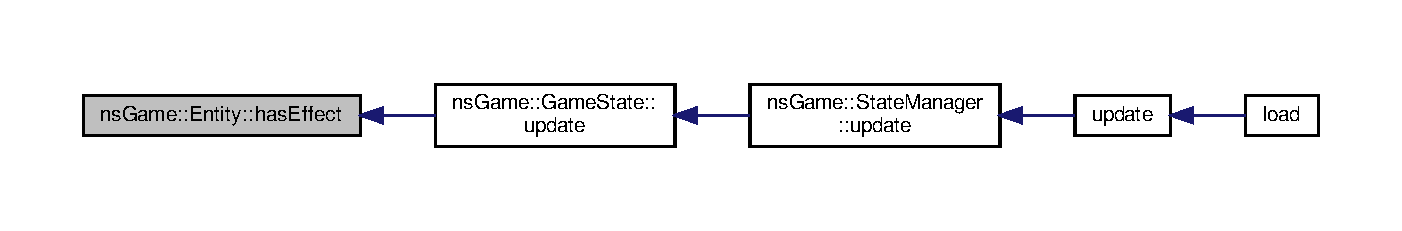
\includegraphics[width=350pt]{structns_game_1_1_entity_af5bf634702f96ed5daac8130a3dee4f0_icgraph}
\end{center}
\end{figure}
\mbox{\Hypertarget{structns_game_1_1_entity_aa0057e4e5b73cc0187602c3180347a3a}\label{structns_game_1_1_entity_aa0057e4e5b73cc0187602c3180347a3a}} 
\index{ns\+Game\+::\+Entity@{ns\+Game\+::\+Entity}!id@{id}}
\index{id@{id}!ns\+Game\+::\+Entity@{ns\+Game\+::\+Entity}}
\subsubsection{\texorpdfstring{id()}{id()}}
{\footnotesize\ttfamily std\+::string Entity\+::id (\begin{DoxyParamCaption}{ }\end{DoxyParamCaption})}



Returns an entity ID, allows the game to set cooldowns or whatever associated with its ID. 

\begin{DoxyReturn}{Returns}
\hyperlink{structns_game_1_1_entity}{Entity} ID 
\end{DoxyReturn}


Definition at line 94 of file entity.\+cpp.

\mbox{\Hypertarget{structns_game_1_1_entity_a5dd00624fa76be09de80a6d2a982ea09}\label{structns_game_1_1_entity_a5dd00624fa76be09de80a6d2a982ea09}} 
\index{ns\+Game\+::\+Entity@{ns\+Game\+::\+Entity}!in\+Collision@{in\+Collision}}
\index{in\+Collision@{in\+Collision}!ns\+Game\+::\+Entity@{ns\+Game\+::\+Entity}}
\subsubsection{\texorpdfstring{in\+Collision()}{inCollision()}}
{\footnotesize\ttfamily bool ns\+Game\+::\+Entity\+::in\+Collision (\begin{DoxyParamCaption}\item[{\hyperlink{type_8h_a64a592133575ccebb1b36453acbec02b}{C\+Mat}}]{map,  }\item[{unsigned}]{x,  }\item[{unsigned}]{y }\end{DoxyParamCaption})}



Checks if entity would be in collision with a structure (walls...) $\vert$ O\+V\+E\+R\+R\+I\+DE IF N\+E\+E\+D\+ED (Flying monsters?) 



Definition at line 65 of file entity.\+cpp.

Here is the caller graph for this function\+:\nopagebreak
\begin{figure}[H]
\begin{center}
\leavevmode
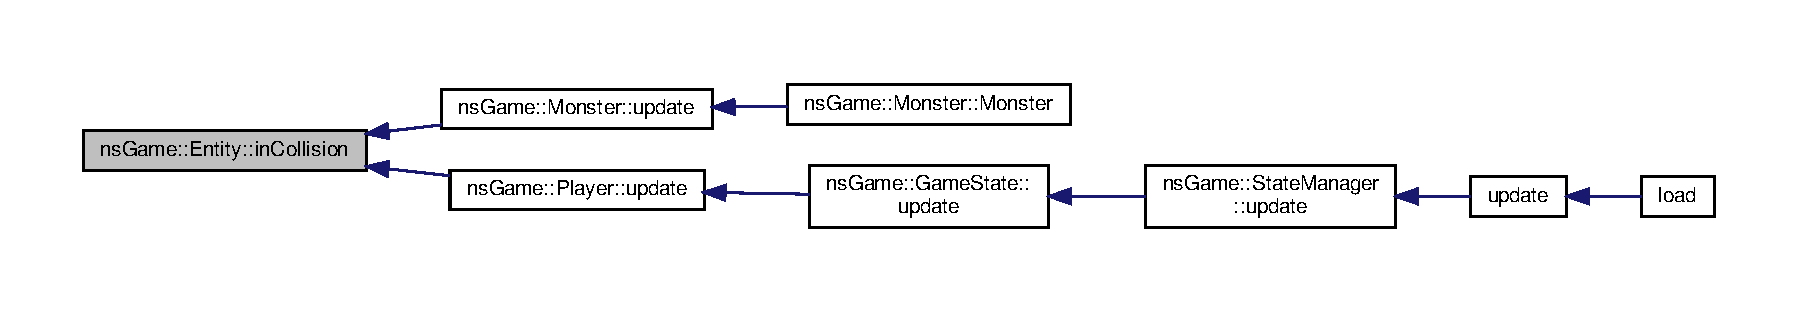
\includegraphics[width=350pt]{structns_game_1_1_entity_a5dd00624fa76be09de80a6d2a982ea09_icgraph}
\end{center}
\end{figure}
\mbox{\Hypertarget{structns_game_1_1_entity_a522648b330daab91b49f78f0737a943f}\label{structns_game_1_1_entity_a522648b330daab91b49f78f0737a943f}} 
\index{ns\+Game\+::\+Entity@{ns\+Game\+::\+Entity}!kill@{kill}}
\index{kill@{kill}!ns\+Game\+::\+Entity@{ns\+Game\+::\+Entity}}
\subsubsection{\texorpdfstring{kill()}{kill()}}
{\footnotesize\ttfamily void Entity\+::kill (\begin{DoxyParamCaption}{ }\end{DoxyParamCaption})}



Definition at line 74 of file entity.\+cpp.

Here is the caller graph for this function\+:\nopagebreak
\begin{figure}[H]
\begin{center}
\leavevmode
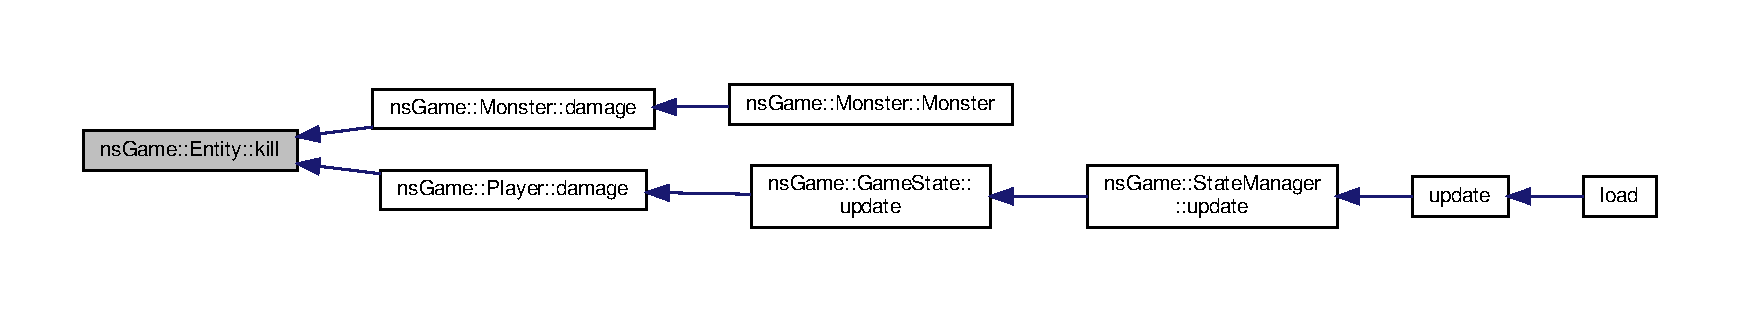
\includegraphics[width=350pt]{structns_game_1_1_entity_a522648b330daab91b49f78f0737a943f_icgraph}
\end{center}
\end{figure}
\mbox{\Hypertarget{structns_game_1_1_entity_ae0aa595447b5f3d2c0b80fb99305c56e}\label{structns_game_1_1_entity_ae0aa595447b5f3d2c0b80fb99305c56e}} 
\index{ns\+Game\+::\+Entity@{ns\+Game\+::\+Entity}!load@{load}}
\index{load@{load}!ns\+Game\+::\+Entity@{ns\+Game\+::\+Entity}}
\subsubsection{\texorpdfstring{load()}{load()}}
{\footnotesize\ttfamily void Entity\+::load (\begin{DoxyParamCaption}{ }\end{DoxyParamCaption})}



load 



Definition at line 16 of file entity.\+cpp.

Here is the caller graph for this function\+:\nopagebreak
\begin{figure}[H]
\begin{center}
\leavevmode
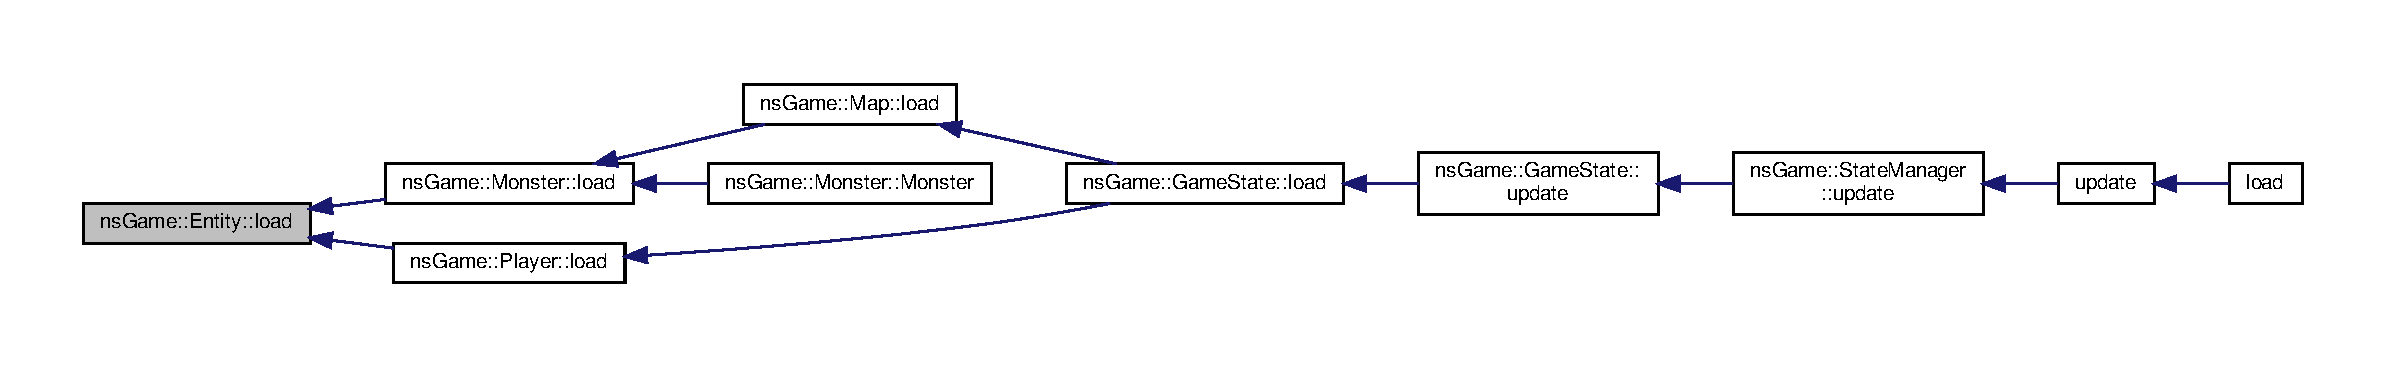
\includegraphics[width=350pt]{structns_game_1_1_entity_ae0aa595447b5f3d2c0b80fb99305c56e_icgraph}
\end{center}
\end{figure}
\mbox{\Hypertarget{structns_game_1_1_entity_accc47c70658884bd70938642fc1cc431}\label{structns_game_1_1_entity_accc47c70658884bd70938642fc1cc431}} 
\index{ns\+Game\+::\+Entity@{ns\+Game\+::\+Entity}!remove\+Effect@{remove\+Effect}}
\index{remove\+Effect@{remove\+Effect}!ns\+Game\+::\+Entity@{ns\+Game\+::\+Entity}}
\subsubsection{\texorpdfstring{remove\+Effect()}{removeEffect()}}
{\footnotesize\ttfamily void Entity\+::remove\+Effect (\begin{DoxyParamCaption}\item[{\hyperlink{namespacens_game_afea521dd2ba8e97be9549ce9936f4522}{Effect\+Type}}]{type }\end{DoxyParamCaption})}



Removes an effect from the entity. 


\begin{DoxyParams}{Parameters}
{\em Effect\+Type} & -\/ Effect ID \\
\hline
{\em Effect} & -\/ Effect \\
\hline
\end{DoxyParams}


Definition at line 107 of file entity.\+cpp.

\mbox{\Hypertarget{structns_game_1_1_entity_a4663cc85381acc9aaac120a85b6f24d0}\label{structns_game_1_1_entity_a4663cc85381acc9aaac120a85b6f24d0}} 
\index{ns\+Game\+::\+Entity@{ns\+Game\+::\+Entity}!render@{render}}
\index{render@{render}!ns\+Game\+::\+Entity@{ns\+Game\+::\+Entity}}
\subsubsection{\texorpdfstring{render()}{render()}}
{\footnotesize\ttfamily void Entity\+::render (\begin{DoxyParamCaption}\item[{Min\+GL \&}]{window }\end{DoxyParamCaption})}



render 


\begin{DoxyParams}{Parameters}
{\em window} & \\
\hline
\end{DoxyParams}


Definition at line 39 of file entity.\+cpp.

Here is the call graph for this function\+:\nopagebreak
\begin{figure}[H]
\begin{center}
\leavevmode
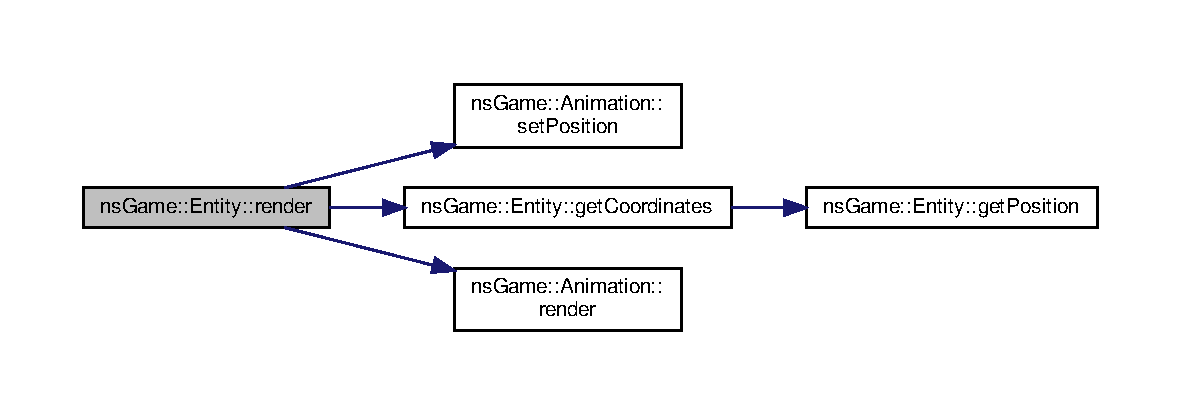
\includegraphics[width=350pt]{structns_game_1_1_entity_a4663cc85381acc9aaac120a85b6f24d0_cgraph}
\end{center}
\end{figure}
Here is the caller graph for this function\+:\nopagebreak
\begin{figure}[H]
\begin{center}
\leavevmode
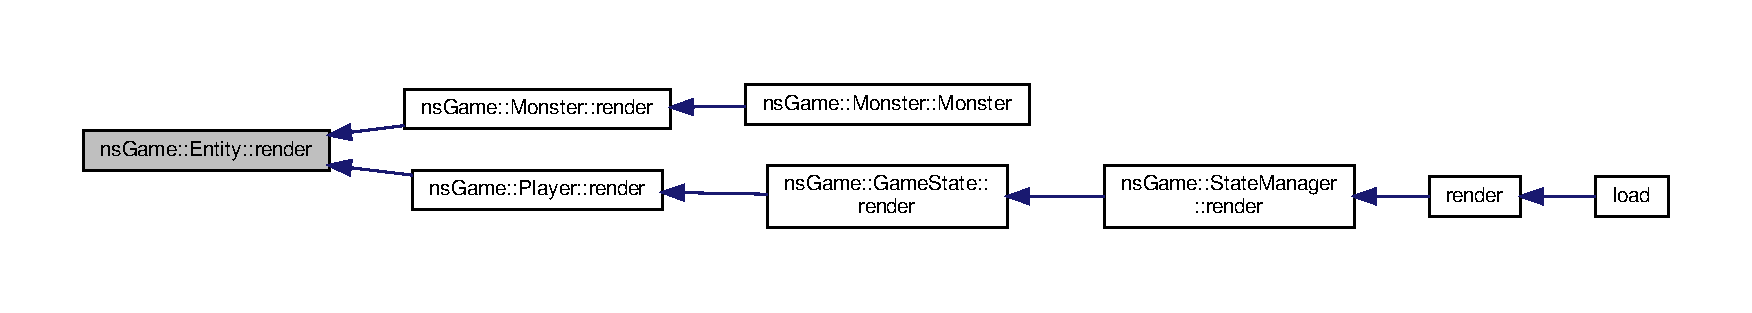
\includegraphics[width=350pt]{structns_game_1_1_entity_a4663cc85381acc9aaac120a85b6f24d0_icgraph}
\end{center}
\end{figure}
\mbox{\Hypertarget{structns_game_1_1_entity_a0254c30b6223caa723303266ad04e4cd}\label{structns_game_1_1_entity_a0254c30b6223caa723303266ad04e4cd}} 
\index{ns\+Game\+::\+Entity@{ns\+Game\+::\+Entity}!set\+Movement\+Speed@{set\+Movement\+Speed}}
\index{set\+Movement\+Speed@{set\+Movement\+Speed}!ns\+Game\+::\+Entity@{ns\+Game\+::\+Entity}}
\subsubsection{\texorpdfstring{set\+Movement\+Speed()}{setMovementSpeed()}}
{\footnotesize\ttfamily void ns\+Game\+::\+Entity\+::set\+Movement\+Speed (\begin{DoxyParamCaption}\item[{double}]{speed }\end{DoxyParamCaption})}



Sets the movement speed. 



Definition at line 98 of file entity.\+cpp.

Here is the call graph for this function\+:\nopagebreak
\begin{figure}[H]
\begin{center}
\leavevmode
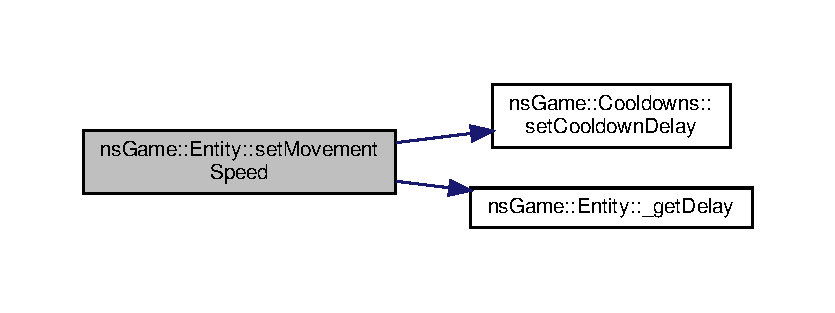
\includegraphics[width=350pt]{structns_game_1_1_entity_a0254c30b6223caa723303266ad04e4cd_cgraph}
\end{center}
\end{figure}
Here is the caller graph for this function\+:\nopagebreak
\begin{figure}[H]
\begin{center}
\leavevmode
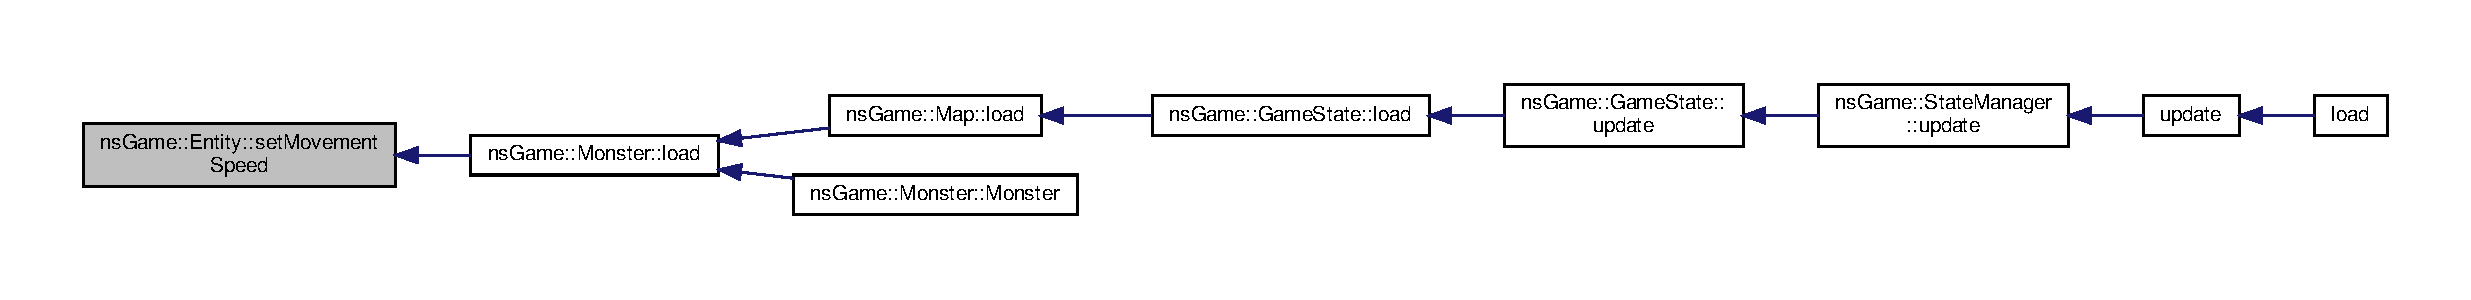
\includegraphics[width=350pt]{structns_game_1_1_entity_a0254c30b6223caa723303266ad04e4cd_icgraph}
\end{center}
\end{figure}
\mbox{\Hypertarget{structns_game_1_1_entity_ac09f45ca50c9fef57a50c4414fc7e20d}\label{structns_game_1_1_entity_ac09f45ca50c9fef57a50c4414fc7e20d}} 
\index{ns\+Game\+::\+Entity@{ns\+Game\+::\+Entity}!spawn@{spawn}}
\index{spawn@{spawn}!ns\+Game\+::\+Entity@{ns\+Game\+::\+Entity}}
\subsubsection{\texorpdfstring{spawn()}{spawn()}}
{\footnotesize\ttfamily void ns\+Game\+::\+Entity\+::spawn (\begin{DoxyParamCaption}{ }\end{DoxyParamCaption})}



Teleports the entity at its spawn. 



Definition at line 85 of file entity.\+cpp.

\mbox{\Hypertarget{structns_game_1_1_entity_af1da5da20798e01469c4a438d0b4174c}\label{structns_game_1_1_entity_af1da5da20798e01469c4a438d0b4174c}} 
\index{ns\+Game\+::\+Entity@{ns\+Game\+::\+Entity}!update@{update}}
\index{update@{update}!ns\+Game\+::\+Entity@{ns\+Game\+::\+Entity}}
\subsubsection{\texorpdfstring{update()}{update()}}
{\footnotesize\ttfamily void Entity\+::update (\begin{DoxyParamCaption}\item[{unsigned}]{delta,  }\item[{\hyperlink{type_8h_a64a592133575ccebb1b36453acbec02b}{C\+Mat} \&}]{mat }\end{DoxyParamCaption})}



update 


\begin{DoxyParams}{Parameters}
{\em delta} & \\
\hline
{\em mat} & \\
\hline
\end{DoxyParams}


Definition at line 24 of file entity.\+cpp.

Here is the call graph for this function\+:\nopagebreak
\begin{figure}[H]
\begin{center}
\leavevmode
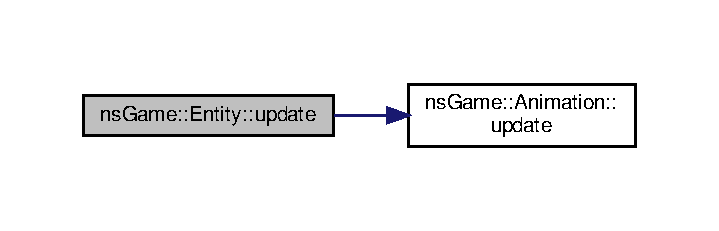
\includegraphics[width=345pt]{structns_game_1_1_entity_af1da5da20798e01469c4a438d0b4174c_cgraph}
\end{center}
\end{figure}
Here is the caller graph for this function\+:\nopagebreak
\begin{figure}[H]
\begin{center}
\leavevmode
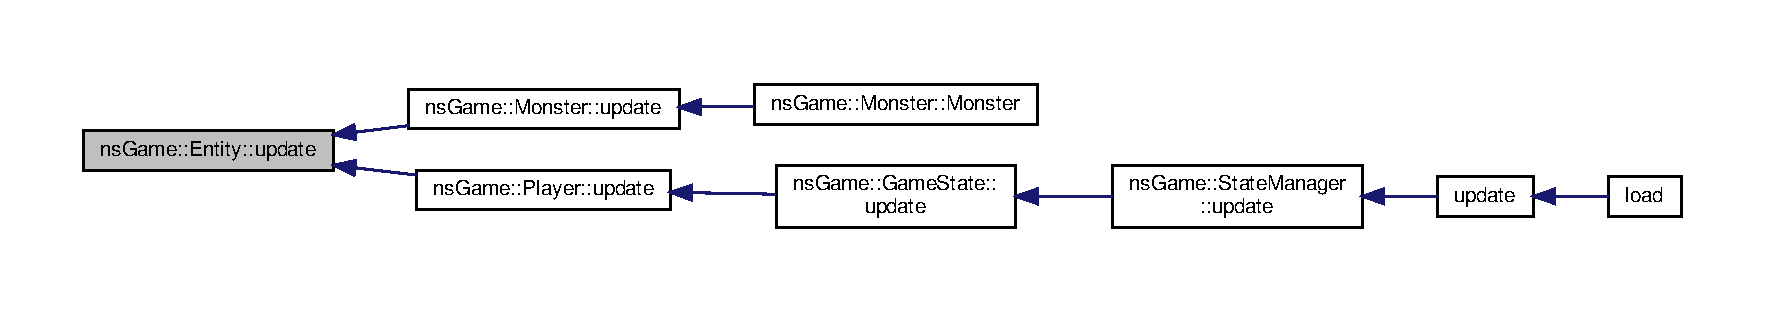
\includegraphics[width=350pt]{structns_game_1_1_entity_af1da5da20798e01469c4a438d0b4174c_icgraph}
\end{center}
\end{figure}


\subsection{Member Data Documentation}
\mbox{\Hypertarget{structns_game_1_1_entity_a3b26c2bf34732b4621932ab7d50421e9}\label{structns_game_1_1_entity_a3b26c2bf34732b4621932ab7d50421e9}} 
\index{ns\+Game\+::\+Entity@{ns\+Game\+::\+Entity}!is\+Allowed\+To\+Move@{is\+Allowed\+To\+Move}}
\index{is\+Allowed\+To\+Move@{is\+Allowed\+To\+Move}!ns\+Game\+::\+Entity@{ns\+Game\+::\+Entity}}
\subsubsection{\texorpdfstring{is\+Allowed\+To\+Move}{isAllowedToMove}}
{\footnotesize\ttfamily bool ns\+Game\+::\+Entity\+::is\+Allowed\+To\+Move = true}



Prevents entity to move. 



Definition at line 42 of file entity.\+h.

\mbox{\Hypertarget{structns_game_1_1_entity_a2b5d83f01bdc1d58673b3fae9afe704e}\label{structns_game_1_1_entity_a2b5d83f01bdc1d58673b3fae9afe704e}} 
\index{ns\+Game\+::\+Entity@{ns\+Game\+::\+Entity}!movement\+Speed@{movement\+Speed}}
\index{movement\+Speed@{movement\+Speed}!ns\+Game\+::\+Entity@{ns\+Game\+::\+Entity}}
\subsubsection{\texorpdfstring{movement\+Speed}{movementSpeed}}
{\footnotesize\ttfamily double ns\+Game\+::\+Entity\+::movement\+Speed = 1.\+0\hspace{0.3cm}{\ttfamily [protected]}}



Movement Speed. 



Definition at line 38 of file entity.\+h.

\mbox{\Hypertarget{structns_game_1_1_entity_a1ad359bb31e86c4971fd96b080ed43c4}\label{structns_game_1_1_entity_a1ad359bb31e86c4971fd96b080ed43c4}} 
\index{ns\+Game\+::\+Entity@{ns\+Game\+::\+Entity}!pos@{pos}}
\index{pos@{pos}!ns\+Game\+::\+Entity@{ns\+Game\+::\+Entity}}
\subsubsection{\texorpdfstring{pos}{pos}}
{\footnotesize\ttfamily ns\+Graphics\+::\+Vec2D ns\+Game\+::\+Entity\+::pos}



\hyperlink{structns_game_1_1_entity}{Entity} position. 



Definition at line 48 of file entity.\+h.

\mbox{\Hypertarget{structns_game_1_1_entity_aaf71fbc10979dcc5b5af55fcb6e44216}\label{structns_game_1_1_entity_aaf71fbc10979dcc5b5af55fcb6e44216}} 
\index{ns\+Game\+::\+Entity@{ns\+Game\+::\+Entity}!slain@{slain}}
\index{slain@{slain}!ns\+Game\+::\+Entity@{ns\+Game\+::\+Entity}}
\subsubsection{\texorpdfstring{slain}{slain}}
{\footnotesize\ttfamily bool ns\+Game\+::\+Entity\+::slain = false}



Says if entity has been killed. 



Definition at line 45 of file entity.\+h.



The documentation for this class was generated from the following files\+:\begin{DoxyCompactItemize}
\item 
Nos\+\_\+fichiers/\hyperlink{entity_8h}{entity.\+h}\item 
Nos\+\_\+fichiers/\hyperlink{entity_8cpp}{entity.\+cpp}\end{DoxyCompactItemize}

\hypertarget{classns_game_1_1_fruit}{}\section{ns\+Game\+:\+:Fruit Class Reference}
\label{classns_game_1_1_fruit}\index{ns\+Game\+::\+Fruit@{ns\+Game\+::\+Fruit}}


Defines \hyperlink{classns_game_1_1_fruit}{Fruit}.  




{\ttfamily \#include $<$fruit.\+h$>$}



Inheritance diagram for ns\+Game\+:\+:Fruit\+:\nopagebreak
\begin{figure}[H]
\begin{center}
\leavevmode
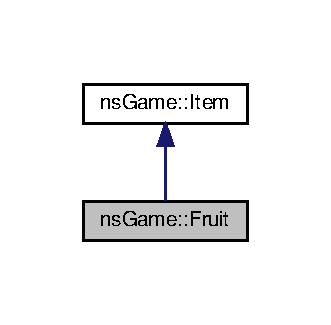
\includegraphics[width=159pt]{classns_game_1_1_fruit__inherit__graph}
\end{center}
\end{figure}


Collaboration diagram for ns\+Game\+:\+:Fruit\+:\nopagebreak
\begin{figure}[H]
\begin{center}
\leavevmode
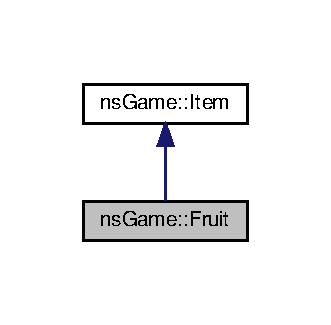
\includegraphics[width=159pt]{classns_game_1_1_fruit__coll__graph}
\end{center}
\end{figure}
\subsection*{Public Member Functions}
\begin{DoxyCompactItemize}
\item 
\hyperlink{classns_game_1_1_fruit_a3d8e8a000d60e2d1f71ebd1820dd6667}{Fruit} (ns\+Graphics\+::\+Vec2D \hyperlink{structns_game_1_1_item_a5518876a13f3d2eda659d29748097f1a}{pos})
\item 
void \hyperlink{classns_game_1_1_fruit_a28c4ae21607dbad699602528c6ffc583}{load} () override
\begin{DoxyCompactList}\small\item\em Loads food. \end{DoxyCompactList}\item 
void \hyperlink{classns_game_1_1_fruit_adade5568e2f552576d0d32b714b9ac02}{update} (unsigned delta) override
\begin{DoxyCompactList}\small\item\em Updates food. \end{DoxyCompactList}\item 
void \hyperlink{classns_game_1_1_fruit_a99622754f8cf90bb285b4808e98372c7}{render} (Min\+GL \&window) override
\begin{DoxyCompactList}\small\item\em Renders resources. \end{DoxyCompactList}\item 
void \hyperlink{classns_game_1_1_fruit_ad33836a67756dba7390b95c57898e91c}{action} (\hyperlink{classns_game_1_1_player}{Player} $\ast$player) override
\begin{DoxyCompactList}\small\item\em Makes an action for the player. \end{DoxyCompactList}\item 
\hyperlink{namespacens_game_a5f7db01e6447720e9a145f0b3c68a4d7}{Item\+Type} \hyperlink{classns_game_1_1_fruit_a4d704f296f536afc2980183bb21e4c62}{get\+Type} () override
\begin{DoxyCompactList}\small\item\em Gets item type. \end{DoxyCompactList}\end{DoxyCompactItemize}
\subsection*{Additional Inherited Members}


\subsection{Detailed Description}
Defines \hyperlink{classns_game_1_1_fruit}{Fruit}. 

\begin{DoxyAuthor}{Authors}
Thomas Cardon 
\end{DoxyAuthor}


Definition at line 25 of file fruit.\+h.



\subsection{Constructor \& Destructor Documentation}
\mbox{\Hypertarget{classns_game_1_1_fruit_a3d8e8a000d60e2d1f71ebd1820dd6667}\label{classns_game_1_1_fruit_a3d8e8a000d60e2d1f71ebd1820dd6667}} 
\index{ns\+Game\+::\+Fruit@{ns\+Game\+::\+Fruit}!Fruit@{Fruit}}
\index{Fruit@{Fruit}!ns\+Game\+::\+Fruit@{ns\+Game\+::\+Fruit}}
\subsubsection{\texorpdfstring{Fruit()}{Fruit()}}
{\footnotesize\ttfamily ns\+Game\+::\+Fruit\+::\+Fruit (\begin{DoxyParamCaption}\item[{ns\+Graphics\+::\+Vec2D}]{pos }\end{DoxyParamCaption})\hspace{0.3cm}{\ttfamily [inline]}}



Definition at line 32 of file fruit.\+h.

Here is the call graph for this function\+:\nopagebreak
\begin{figure}[H]
\begin{center}
\leavevmode
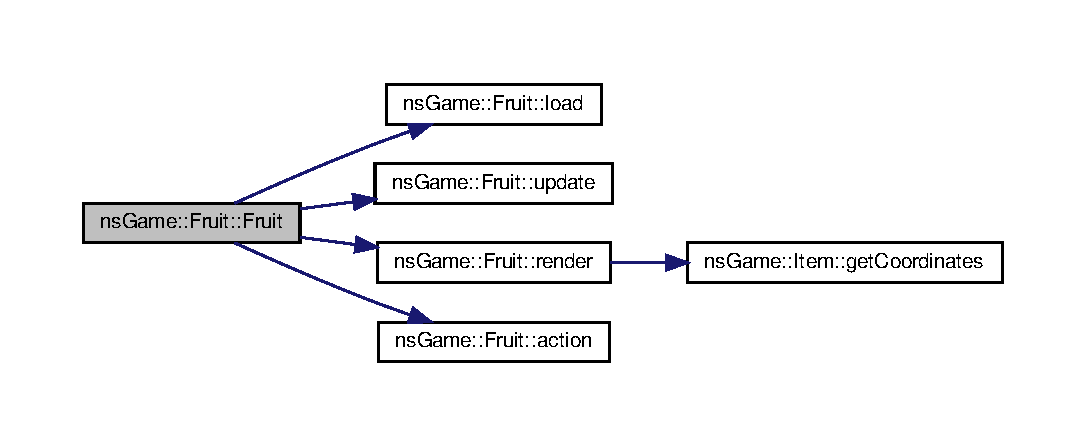
\includegraphics[width=350pt]{classns_game_1_1_fruit_a3d8e8a000d60e2d1f71ebd1820dd6667_cgraph}
\end{center}
\end{figure}


\subsection{Member Function Documentation}
\mbox{\Hypertarget{classns_game_1_1_fruit_ad33836a67756dba7390b95c57898e91c}\label{classns_game_1_1_fruit_ad33836a67756dba7390b95c57898e91c}} 
\index{ns\+Game\+::\+Fruit@{ns\+Game\+::\+Fruit}!action@{action}}
\index{action@{action}!ns\+Game\+::\+Fruit@{ns\+Game\+::\+Fruit}}
\subsubsection{\texorpdfstring{action()}{action()}}
{\footnotesize\ttfamily void Fruit\+::action (\begin{DoxyParamCaption}\item[{\hyperlink{classns_game_1_1_player}{Player} $\ast$}]{player }\end{DoxyParamCaption})\hspace{0.3cm}{\ttfamily [override]}, {\ttfamily [virtual]}}



Makes an action for the player. 


\begin{DoxyParams}{Parameters}
{\em \hyperlink{classns_game_1_1_player}{Player}} & -\/ The player that steps on an item \\
\hline
\end{DoxyParams}


Implements \hyperlink{structns_game_1_1_item_af74dffcf9bde4a4297749f4e1852395b}{ns\+Game\+::\+Item}.



Definition at line 22 of file fruit.\+cpp.

Here is the caller graph for this function\+:\nopagebreak
\begin{figure}[H]
\begin{center}
\leavevmode
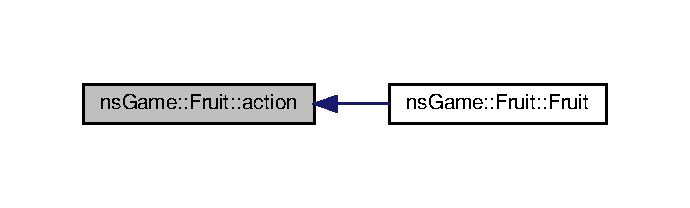
\includegraphics[width=331pt]{classns_game_1_1_fruit_ad33836a67756dba7390b95c57898e91c_icgraph}
\end{center}
\end{figure}
\mbox{\Hypertarget{classns_game_1_1_fruit_a4d704f296f536afc2980183bb21e4c62}\label{classns_game_1_1_fruit_a4d704f296f536afc2980183bb21e4c62}} 
\index{ns\+Game\+::\+Fruit@{ns\+Game\+::\+Fruit}!get\+Type@{get\+Type}}
\index{get\+Type@{get\+Type}!ns\+Game\+::\+Fruit@{ns\+Game\+::\+Fruit}}
\subsubsection{\texorpdfstring{get\+Type()}{getType()}}
{\footnotesize\ttfamily \hyperlink{namespacens_game_a5f7db01e6447720e9a145f0b3c68a4d7}{Item\+Type} ns\+Game\+::\+Fruit\+::get\+Type (\begin{DoxyParamCaption}{ }\end{DoxyParamCaption})\hspace{0.3cm}{\ttfamily [inline]}, {\ttfamily [override]}, {\ttfamily [virtual]}}



Gets item type. 

\begin{DoxyReturn}{Returns}
Item\+Type.\+I\+T\+EM 
\end{DoxyReturn}


Reimplemented from \hyperlink{structns_game_1_1_item_a69156550e5083928cbb673ca2db671f5}{ns\+Game\+::\+Item}.



Definition at line 62 of file fruit.\+h.

\mbox{\Hypertarget{classns_game_1_1_fruit_a28c4ae21607dbad699602528c6ffc583}\label{classns_game_1_1_fruit_a28c4ae21607dbad699602528c6ffc583}} 
\index{ns\+Game\+::\+Fruit@{ns\+Game\+::\+Fruit}!load@{load}}
\index{load@{load}!ns\+Game\+::\+Fruit@{ns\+Game\+::\+Fruit}}
\subsubsection{\texorpdfstring{load()}{load()}}
{\footnotesize\ttfamily void ns\+Game\+::\+Fruit\+::load (\begin{DoxyParamCaption}{ }\end{DoxyParamCaption})\hspace{0.3cm}{\ttfamily [override]}, {\ttfamily [virtual]}}



Loads food. 



Implements \hyperlink{structns_game_1_1_item_a5887b6e9225ae8a276801225eca83808}{ns\+Game\+::\+Item}.



Definition at line 16 of file fruit.\+cpp.

Here is the caller graph for this function\+:\nopagebreak
\begin{figure}[H]
\begin{center}
\leavevmode
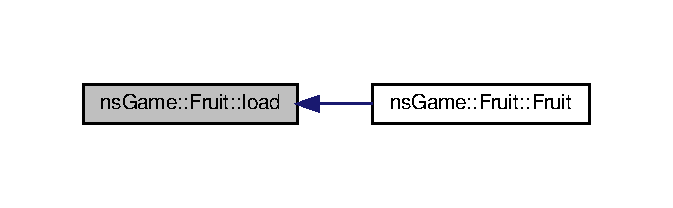
\includegraphics[width=323pt]{classns_game_1_1_fruit_a28c4ae21607dbad699602528c6ffc583_icgraph}
\end{center}
\end{figure}
\mbox{\Hypertarget{classns_game_1_1_fruit_a99622754f8cf90bb285b4808e98372c7}\label{classns_game_1_1_fruit_a99622754f8cf90bb285b4808e98372c7}} 
\index{ns\+Game\+::\+Fruit@{ns\+Game\+::\+Fruit}!render@{render}}
\index{render@{render}!ns\+Game\+::\+Fruit@{ns\+Game\+::\+Fruit}}
\subsubsection{\texorpdfstring{render()}{render()}}
{\footnotesize\ttfamily void ns\+Game\+::\+Fruit\+::render (\begin{DoxyParamCaption}\item[{Min\+GL \&}]{window }\end{DoxyParamCaption})\hspace{0.3cm}{\ttfamily [override]}, {\ttfamily [virtual]}}



Renders resources. 



Implements \hyperlink{structns_game_1_1_item_a451b6491efc475c9ca47dcccdbbde707}{ns\+Game\+::\+Item}.



Definition at line 27 of file fruit.\+cpp.

Here is the call graph for this function\+:\nopagebreak
\begin{figure}[H]
\begin{center}
\leavevmode
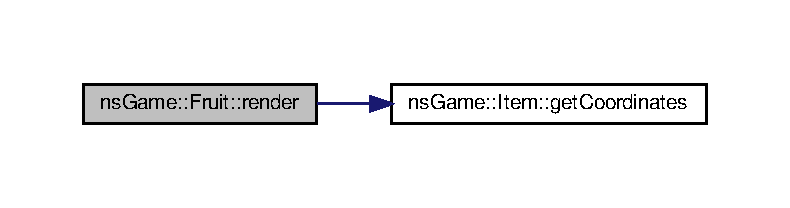
\includegraphics[width=350pt]{classns_game_1_1_fruit_a99622754f8cf90bb285b4808e98372c7_cgraph}
\end{center}
\end{figure}
Here is the caller graph for this function\+:\nopagebreak
\begin{figure}[H]
\begin{center}
\leavevmode
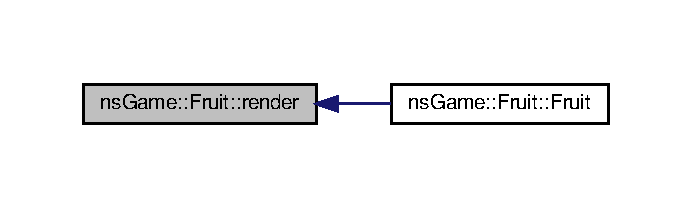
\includegraphics[width=332pt]{classns_game_1_1_fruit_a99622754f8cf90bb285b4808e98372c7_icgraph}
\end{center}
\end{figure}
\mbox{\Hypertarget{classns_game_1_1_fruit_adade5568e2f552576d0d32b714b9ac02}\label{classns_game_1_1_fruit_adade5568e2f552576d0d32b714b9ac02}} 
\index{ns\+Game\+::\+Fruit@{ns\+Game\+::\+Fruit}!update@{update}}
\index{update@{update}!ns\+Game\+::\+Fruit@{ns\+Game\+::\+Fruit}}
\subsubsection{\texorpdfstring{update()}{update()}}
{\footnotesize\ttfamily void ns\+Game\+::\+Fruit\+::update (\begin{DoxyParamCaption}\item[{unsigned}]{delta }\end{DoxyParamCaption})\hspace{0.3cm}{\ttfamily [override]}, {\ttfamily [virtual]}}



Updates food. 



Implements \hyperlink{structns_game_1_1_item_a96c07d0f91eef0d77e91d1a7397091a1}{ns\+Game\+::\+Item}.



Definition at line 20 of file fruit.\+cpp.

Here is the caller graph for this function\+:\nopagebreak
\begin{figure}[H]
\begin{center}
\leavevmode
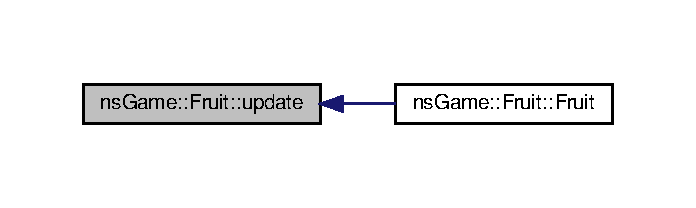
\includegraphics[width=334pt]{classns_game_1_1_fruit_adade5568e2f552576d0d32b714b9ac02_icgraph}
\end{center}
\end{figure}


The documentation for this class was generated from the following files\+:\begin{DoxyCompactItemize}
\item 
Nos\+\_\+fichiers/\hyperlink{fruit_8h}{fruit.\+h}\item 
Nos\+\_\+fichiers/\hyperlink{fruit_8cpp}{fruit.\+cpp}\end{DoxyCompactItemize}

\hypertarget{classns_game_1_1_game_state}{}\section{ns\+Game\+:\+:Game\+State Class Reference}
\label{classns_game_1_1_game_state}\index{ns\+Game\+::\+Game\+State@{ns\+Game\+::\+Game\+State}}


Defines the game logic.  




{\ttfamily \#include $<$game\+State.\+h$>$}



Inheritance diagram for ns\+Game\+:\+:Game\+State\+:\nopagebreak
\begin{figure}[H]
\begin{center}
\leavevmode
\includegraphics[width=189pt]{classns_game_1_1_game_state__inherit__graph}
\end{center}
\end{figure}


Collaboration diagram for ns\+Game\+:\+:Game\+State\+:\nopagebreak
\begin{figure}[H]
\begin{center}
\leavevmode
\includegraphics[width=350pt]{classns_game_1_1_game_state__coll__graph}
\end{center}
\end{figure}
\subsection*{Public Member Functions}
\begin{DoxyCompactItemize}
\item 
virtual void \hyperlink{classns_game_1_1_game_state_a66f7b8027a33f473fd22c212700586f2}{load} () override
\begin{DoxyCompactList}\small\item\em Loads \hyperlink{structns_game_1_1_state}{State} resources. \end{DoxyCompactList}\item 
virtual void \hyperlink{classns_game_1_1_game_state_ac0fdc8e463ca2e79a0fb58e12e5b39c9}{destroy} () override
\begin{DoxyCompactList}\small\item\em Destroys state (and resets it) \end{DoxyCompactList}\item 
virtual void \hyperlink{classns_game_1_1_game_state_a4d3cb871a1aec541a37fe241664b738c}{update} (Min\+GL \&window, unsigned delta) override
\begin{DoxyCompactList}\small\item\em Updates state. \end{DoxyCompactList}\item 
void \hyperlink{classns_game_1_1_game_state_a78176e52c8f3c745bb88a4214f5aa29b}{check\+For\+Win} (\hyperlink{classns_game_1_1_player}{Player} $\ast$p1, \hyperlink{classns_game_1_1_player}{Player} $\ast$p2)
\begin{DoxyCompactList}\small\item\em Checks every tick (\hyperlink{structns_game_1_1_state_ae809e89ac9df4a43ab90d5d5932e2bc7}{State\+::update()}) if one of the players have won (or not). \end{DoxyCompactList}\item 
virtual void \hyperlink{classns_game_1_1_game_state_a1e3179b016431332ecff880e09e267d3}{render} (Min\+GL \&window) override
\begin{DoxyCompactList}\small\item\em Renders resources. \end{DoxyCompactList}\item 
void \hyperlink{classns_game_1_1_game_state_a8d9cadd7432dfd4b7ada08e37bf6b30d}{render\+Score} (Min\+GL \&window, \hyperlink{classns_game_1_1_player}{Player} p)
\begin{DoxyCompactList}\small\item\em Renders the score on the sidebar for a given player. \end{DoxyCompactList}\item 
void \hyperlink{classns_game_1_1_game_state_a66f328c56ed9887e02a93db856316d4c}{render\+Victory\+Screen} (Min\+GL \&window)
\begin{DoxyCompactList}\small\item\em Renders the victory screen. \end{DoxyCompactList}\end{DoxyCompactItemize}
\subsection*{Public Attributes}
\begin{DoxyCompactItemize}
\item 
int \hyperlink{classns_game_1_1_game_state_aa5b4cb6af0e806d442e5291578a6822a}{win} = -\/1
\begin{DoxyCompactList}\small\item\em Victory status\+: -\/1 = not yet, 0 = equal, 1 = player 1, 2 = player 2. \end{DoxyCompactList}\item 
\hyperlink{classns_game_1_1_map}{Map} $\ast$ \hyperlink{classns_game_1_1_game_state_a451982a5efe66e5402402ed0f996fca6}{map}
\begin{DoxyCompactList}\small\item\em The game map, and its grid. \end{DoxyCompactList}\item 
\hyperlink{struct_c_my_param}{C\+My\+Param} \hyperlink{classns_game_1_1_game_state_a972d8482f9ed69d536ff8c7927a8c290}{Params}
\begin{DoxyCompactList}\small\item\em The game configuration file. \end{DoxyCompactList}\item 
\hyperlink{classns_game_1_1_player}{Player} $\ast$ \hyperlink{classns_game_1_1_game_state_aec14e8ba226edc828deabb6e6b276c70}{player1}
\begin{DoxyCompactList}\small\item\em Players. \end{DoxyCompactList}\item 
\hyperlink{classns_game_1_1_player}{Player} $\ast$ \hyperlink{classns_game_1_1_game_state_abd99551650ebb05056576dd2fee40b4b}{player2}
\item 
ns\+Audio\+::\+Audio\+Engine \hyperlink{classns_game_1_1_game_state_a9bd618bc831669e078759402caa0cb78}{audio}
\begin{DoxyCompactList}\small\item\em min\+GL 2 audio engine \end{DoxyCompactList}\item 
ns\+Gui\+::\+Sprite \hyperlink{classns_game_1_1_game_state_a144f7f71a2a43f8422a346e4bc9bb923}{sidebar} = ns\+Gui\+::\+Sprite(\hyperlink{definitions_8h_a793644bd88146828177a2a4f57e3bf01}{R\+E\+S\+\_\+\+P\+A\+TH} + \char`\"{}/gui/sidebar/panel.\+i2s\char`\"{})
\begin{DoxyCompactList}\small\item\em Sidebar resources. \end{DoxyCompactList}\item 
ns\+Gui\+::\+Sprite \hyperlink{classns_game_1_1_game_state_afaac1bf595eef244503f5b15917e230d}{h0} = ns\+Gui\+::\+Sprite(\hyperlink{definitions_8h_a793644bd88146828177a2a4f57e3bf01}{R\+E\+S\+\_\+\+P\+A\+TH} + \char`\"{}/gui/\hyperlink{classns_game_1_1_game_state_a144f7f71a2a43f8422a346e4bc9bb923}{sidebar}/hearts\+\_\+0.\+i2s\char`\"{})
\item 
ns\+Gui\+::\+Sprite \hyperlink{classns_game_1_1_game_state_a7d9cc08964a619c0f72a7000fe7f511c}{h1} = ns\+Gui\+::\+Sprite(\hyperlink{definitions_8h_a793644bd88146828177a2a4f57e3bf01}{R\+E\+S\+\_\+\+P\+A\+TH} + \char`\"{}/gui/\hyperlink{classns_game_1_1_game_state_a144f7f71a2a43f8422a346e4bc9bb923}{sidebar}/hearts\+\_\+1.\+i2s\char`\"{})
\item 
ns\+Gui\+::\+Sprite \hyperlink{classns_game_1_1_game_state_a1fbc7862058993d3ff53db6f50d3949d}{h2} = ns\+Gui\+::\+Sprite(\hyperlink{definitions_8h_a793644bd88146828177a2a4f57e3bf01}{R\+E\+S\+\_\+\+P\+A\+TH} + \char`\"{}/gui/\hyperlink{classns_game_1_1_game_state_a144f7f71a2a43f8422a346e4bc9bb923}{sidebar}/hearts\+\_\+2.\+i2s\char`\"{})
\item 
ns\+Gui\+::\+Sprite \hyperlink{classns_game_1_1_game_state_a421981b496870032de67b556f80ed1c9}{h3} = ns\+Gui\+::\+Sprite(\hyperlink{definitions_8h_a793644bd88146828177a2a4f57e3bf01}{R\+E\+S\+\_\+\+P\+A\+TH} + \char`\"{}/gui/\hyperlink{classns_game_1_1_game_state_a144f7f71a2a43f8422a346e4bc9bb923}{sidebar}/hearts\+\_\+3.\+i2s\char`\"{})
\item 
ns\+Gui\+::\+Sprite \hyperlink{classns_game_1_1_game_state_a23ea4a0acc9d2f56f9c324ccfa6560ec}{victory\+Screen1} = ns\+Gui\+::\+Sprite(\hyperlink{definitions_8h_a793644bd88146828177a2a4f57e3bf01}{R\+E\+S\+\_\+\+P\+A\+TH} + \char`\"{}/gui/victory\+\_\+screen/player1.\+i2s\char`\"{})
\begin{DoxyCompactList}\small\item\em Victory screens. \end{DoxyCompactList}\item 
ns\+Gui\+::\+Sprite \hyperlink{classns_game_1_1_game_state_ab94cabb5a2665d1afc31937b84880b6e}{victory\+Screen2} = ns\+Gui\+::\+Sprite(\hyperlink{definitions_8h_a793644bd88146828177a2a4f57e3bf01}{R\+E\+S\+\_\+\+P\+A\+TH} + \char`\"{}/gui/victory\+\_\+screen/player2.\+i2s\char`\"{})
\item 
ns\+Gui\+::\+Sprite \hyperlink{classns_game_1_1_game_state_aa0eafc52f02691494625a63ad62cf7db}{equal\+Screen} = ns\+Gui\+::\+Sprite(\hyperlink{definitions_8h_a793644bd88146828177a2a4f57e3bf01}{R\+E\+S\+\_\+\+P\+A\+TH} + \char`\"{}/gui/victory\+\_\+screen/equal.\+i2s\char`\"{})
\item 
std\+::vector$<$ ns\+Gui\+::\+Sprite $\ast$ $>$ \hyperlink{classns_game_1_1_game_state_a0b870e02f74c266d4a03dbe9210f7678}{numbers}
\begin{DoxyCompactList}\small\item\em Set of numbers from 0 to 9, used for the scoreboard, since min\+GL 2 doesn\textquotesingle{}t allow custom fonts... \end{DoxyCompactList}\end{DoxyCompactItemize}


\subsection{Detailed Description}
Defines the game logic. 

\begin{DoxyAuthor}{Author}
Thomas Cardon, Alexandre Arniaud, Angèle Derrives, Mohamed Labidi, Ines Hamidi 
\end{DoxyAuthor}


Definition at line 30 of file game\+State.\+h.



\subsection{Member Function Documentation}
\mbox{\Hypertarget{classns_game_1_1_game_state_a78176e52c8f3c745bb88a4214f5aa29b}\label{classns_game_1_1_game_state_a78176e52c8f3c745bb88a4214f5aa29b}} 
\index{ns\+Game\+::\+Game\+State@{ns\+Game\+::\+Game\+State}!check\+For\+Win@{check\+For\+Win}}
\index{check\+For\+Win@{check\+For\+Win}!ns\+Game\+::\+Game\+State@{ns\+Game\+::\+Game\+State}}
\subsubsection{\texorpdfstring{check\+For\+Win()}{checkForWin()}}
{\footnotesize\ttfamily void ns\+Game\+::\+Game\+State\+::check\+For\+Win (\begin{DoxyParamCaption}\item[{\hyperlink{classns_game_1_1_player}{Player} $\ast$}]{p1,  }\item[{\hyperlink{classns_game_1_1_player}{Player} $\ast$}]{p2 }\end{DoxyParamCaption})}



Checks every tick (\hyperlink{structns_game_1_1_state_ae809e89ac9df4a43ab90d5d5932e2bc7}{State\+::update()}) if one of the players have won (or not). 


\begin{DoxyParams}{Parameters}
{\em \hyperlink{classns_game_1_1_player}{Player}} & player1 -\/ Le joueur 1 \\
\hline
{\em \hyperlink{classns_game_1_1_player}{Player}} & player2 -\/ Le joueur 2 \\
\hline
\end{DoxyParams}


Definition at line 58 of file game\+State.\+cpp.

Here is the caller graph for this function\+:\nopagebreak
\begin{figure}[H]
\begin{center}
\leavevmode
\includegraphics[width=350pt]{classns_game_1_1_game_state_a78176e52c8f3c745bb88a4214f5aa29b_icgraph}
\end{center}
\end{figure}
\mbox{\Hypertarget{classns_game_1_1_game_state_ac0fdc8e463ca2e79a0fb58e12e5b39c9}\label{classns_game_1_1_game_state_ac0fdc8e463ca2e79a0fb58e12e5b39c9}} 
\index{ns\+Game\+::\+Game\+State@{ns\+Game\+::\+Game\+State}!destroy@{destroy}}
\index{destroy@{destroy}!ns\+Game\+::\+Game\+State@{ns\+Game\+::\+Game\+State}}
\subsubsection{\texorpdfstring{destroy()}{destroy()}}
{\footnotesize\ttfamily void ns\+Game\+::\+Game\+State\+::destroy (\begin{DoxyParamCaption}{ }\end{DoxyParamCaption})\hspace{0.3cm}{\ttfamily [override]}, {\ttfamily [virtual]}}



Destroys state (and resets it) 



Reimplemented from \hyperlink{structns_game_1_1_state_a70a0cf146071a8f9fcb8ca0b2c0f8f44}{ns\+Game\+::\+State}.



Definition at line 47 of file game\+State.\+cpp.

Here is the caller graph for this function\+:\nopagebreak
\begin{figure}[H]
\begin{center}
\leavevmode
\includegraphics[width=350pt]{classns_game_1_1_game_state_ac0fdc8e463ca2e79a0fb58e12e5b39c9_icgraph}
\end{center}
\end{figure}
\mbox{\Hypertarget{classns_game_1_1_game_state_a66f7b8027a33f473fd22c212700586f2}\label{classns_game_1_1_game_state_a66f7b8027a33f473fd22c212700586f2}} 
\index{ns\+Game\+::\+Game\+State@{ns\+Game\+::\+Game\+State}!load@{load}}
\index{load@{load}!ns\+Game\+::\+Game\+State@{ns\+Game\+::\+Game\+State}}
\subsubsection{\texorpdfstring{load()}{load()}}
{\footnotesize\ttfamily void ns\+Game\+::\+Game\+State\+::load (\begin{DoxyParamCaption}{ }\end{DoxyParamCaption})\hspace{0.3cm}{\ttfamily [override]}, {\ttfamily [virtual]}}



Loads \hyperlink{structns_game_1_1_state}{State} resources. 



Reimplemented from \hyperlink{structns_game_1_1_state_a8644de505f7a84933f6d6e6651205791}{ns\+Game\+::\+State}.



Definition at line 14 of file game\+State.\+cpp.

Here is the call graph for this function\+:\nopagebreak
\begin{figure}[H]
\begin{center}
\leavevmode
\includegraphics[width=350pt]{classns_game_1_1_game_state_a66f7b8027a33f473fd22c212700586f2_cgraph}
\end{center}
\end{figure}
Here is the caller graph for this function\+:\nopagebreak
\begin{figure}[H]
\begin{center}
\leavevmode
\includegraphics[width=350pt]{classns_game_1_1_game_state_a66f7b8027a33f473fd22c212700586f2_icgraph}
\end{center}
\end{figure}
\mbox{\Hypertarget{classns_game_1_1_game_state_a1e3179b016431332ecff880e09e267d3}\label{classns_game_1_1_game_state_a1e3179b016431332ecff880e09e267d3}} 
\index{ns\+Game\+::\+Game\+State@{ns\+Game\+::\+Game\+State}!render@{render}}
\index{render@{render}!ns\+Game\+::\+Game\+State@{ns\+Game\+::\+Game\+State}}
\subsubsection{\texorpdfstring{render()}{render()}}
{\footnotesize\ttfamily void ns\+Game\+::\+Game\+State\+::render (\begin{DoxyParamCaption}\item[{Min\+GL \&}]{window }\end{DoxyParamCaption})\hspace{0.3cm}{\ttfamily [override]}, {\ttfamily [virtual]}}



Renders resources. 



Reimplemented from \hyperlink{structns_game_1_1_state_a214f8ee52de4b318f1ed3861a578ce67}{ns\+Game\+::\+State}.



Definition at line 172 of file game\+State.\+cpp.

Here is the call graph for this function\+:\nopagebreak
\begin{figure}[H]
\begin{center}
\leavevmode
\includegraphics[width=350pt]{classns_game_1_1_game_state_a1e3179b016431332ecff880e09e267d3_cgraph}
\end{center}
\end{figure}
Here is the caller graph for this function\+:\nopagebreak
\begin{figure}[H]
\begin{center}
\leavevmode
\includegraphics[width=350pt]{classns_game_1_1_game_state_a1e3179b016431332ecff880e09e267d3_icgraph}
\end{center}
\end{figure}
\mbox{\Hypertarget{classns_game_1_1_game_state_a8d9cadd7432dfd4b7ada08e37bf6b30d}\label{classns_game_1_1_game_state_a8d9cadd7432dfd4b7ada08e37bf6b30d}} 
\index{ns\+Game\+::\+Game\+State@{ns\+Game\+::\+Game\+State}!render\+Score@{render\+Score}}
\index{render\+Score@{render\+Score}!ns\+Game\+::\+Game\+State@{ns\+Game\+::\+Game\+State}}
\subsubsection{\texorpdfstring{render\+Score()}{renderScore()}}
{\footnotesize\ttfamily void ns\+Game\+::\+Game\+State\+::render\+Score (\begin{DoxyParamCaption}\item[{Min\+GL \&}]{window,  }\item[{\hyperlink{classns_game_1_1_player}{Player}}]{p }\end{DoxyParamCaption})}



Renders the score on the sidebar for a given player. 


\begin{DoxyParams}{Parameters}
{\em Min\+GL} & \& window \\
\hline
{\em \hyperlink{classns_game_1_1_player}{Player}} & p \\
\hline
\end{DoxyParams}


Definition at line 153 of file game\+State.\+cpp.

Here is the caller graph for this function\+:\nopagebreak
\begin{figure}[H]
\begin{center}
\leavevmode
\includegraphics[width=350pt]{classns_game_1_1_game_state_a8d9cadd7432dfd4b7ada08e37bf6b30d_icgraph}
\end{center}
\end{figure}
\mbox{\Hypertarget{classns_game_1_1_game_state_a66f328c56ed9887e02a93db856316d4c}\label{classns_game_1_1_game_state_a66f328c56ed9887e02a93db856316d4c}} 
\index{ns\+Game\+::\+Game\+State@{ns\+Game\+::\+Game\+State}!render\+Victory\+Screen@{render\+Victory\+Screen}}
\index{render\+Victory\+Screen@{render\+Victory\+Screen}!ns\+Game\+::\+Game\+State@{ns\+Game\+::\+Game\+State}}
\subsubsection{\texorpdfstring{render\+Victory\+Screen()}{renderVictoryScreen()}}
{\footnotesize\ttfamily void ns\+Game\+::\+Game\+State\+::render\+Victory\+Screen (\begin{DoxyParamCaption}\item[{Min\+GL \&}]{window }\end{DoxyParamCaption})}



Renders the victory screen. 


\begin{DoxyParams}{Parameters}
{\em Min\+GL} & \& window \\
\hline
\end{DoxyParams}


Definition at line 166 of file game\+State.\+cpp.

Here is the caller graph for this function\+:\nopagebreak
\begin{figure}[H]
\begin{center}
\leavevmode
\includegraphics[width=350pt]{classns_game_1_1_game_state_a66f328c56ed9887e02a93db856316d4c_icgraph}
\end{center}
\end{figure}
\mbox{\Hypertarget{classns_game_1_1_game_state_a4d3cb871a1aec541a37fe241664b738c}\label{classns_game_1_1_game_state_a4d3cb871a1aec541a37fe241664b738c}} 
\index{ns\+Game\+::\+Game\+State@{ns\+Game\+::\+Game\+State}!update@{update}}
\index{update@{update}!ns\+Game\+::\+Game\+State@{ns\+Game\+::\+Game\+State}}
\subsubsection{\texorpdfstring{update()}{update()}}
{\footnotesize\ttfamily int ns\+Game\+::\+Game\+State\+::update (\begin{DoxyParamCaption}\item[{Min\+GL \&}]{window,  }\item[{unsigned}]{delta }\end{DoxyParamCaption})\hspace{0.3cm}{\ttfamily [override]}, {\ttfamily [virtual]}}



Updates state. 



Reimplemented from \hyperlink{structns_game_1_1_state_ae809e89ac9df4a43ab90d5d5932e2bc7}{ns\+Game\+::\+State}.



Definition at line 74 of file game\+State.\+cpp.

Here is the call graph for this function\+:\nopagebreak
\begin{figure}[H]
\begin{center}
\leavevmode
\includegraphics[width=350pt]{classns_game_1_1_game_state_a4d3cb871a1aec541a37fe241664b738c_cgraph}
\end{center}
\end{figure}
Here is the caller graph for this function\+:\nopagebreak
\begin{figure}[H]
\begin{center}
\leavevmode
\includegraphics[width=350pt]{classns_game_1_1_game_state_a4d3cb871a1aec541a37fe241664b738c_icgraph}
\end{center}
\end{figure}


\subsection{Member Data Documentation}
\mbox{\Hypertarget{classns_game_1_1_game_state_a9bd618bc831669e078759402caa0cb78}\label{classns_game_1_1_game_state_a9bd618bc831669e078759402caa0cb78}} 
\index{ns\+Game\+::\+Game\+State@{ns\+Game\+::\+Game\+State}!audio@{audio}}
\index{audio@{audio}!ns\+Game\+::\+Game\+State@{ns\+Game\+::\+Game\+State}}
\subsubsection{\texorpdfstring{audio}{audio}}
{\footnotesize\ttfamily ns\+Audio\+::\+Audio\+Engine ns\+Game\+::\+Game\+State\+::audio}



min\+GL 2 audio engine 



Definition at line 46 of file game\+State.\+h.

\mbox{\Hypertarget{classns_game_1_1_game_state_aa0eafc52f02691494625a63ad62cf7db}\label{classns_game_1_1_game_state_aa0eafc52f02691494625a63ad62cf7db}} 
\index{ns\+Game\+::\+Game\+State@{ns\+Game\+::\+Game\+State}!equal\+Screen@{equal\+Screen}}
\index{equal\+Screen@{equal\+Screen}!ns\+Game\+::\+Game\+State@{ns\+Game\+::\+Game\+State}}
\subsubsection{\texorpdfstring{equal\+Screen}{equalScreen}}
{\footnotesize\ttfamily ns\+Gui\+::\+Sprite ns\+Game\+::\+Game\+State\+::equal\+Screen = ns\+Gui\+::\+Sprite(\hyperlink{definitions_8h_a793644bd88146828177a2a4f57e3bf01}{R\+E\+S\+\_\+\+P\+A\+TH} + \char`\"{}/gui/victory\+\_\+screen/equal.\+i2s\char`\"{})}



Definition at line 58 of file game\+State.\+h.

\mbox{\Hypertarget{classns_game_1_1_game_state_afaac1bf595eef244503f5b15917e230d}\label{classns_game_1_1_game_state_afaac1bf595eef244503f5b15917e230d}} 
\index{ns\+Game\+::\+Game\+State@{ns\+Game\+::\+Game\+State}!h0@{h0}}
\index{h0@{h0}!ns\+Game\+::\+Game\+State@{ns\+Game\+::\+Game\+State}}
\subsubsection{\texorpdfstring{h0}{h0}}
{\footnotesize\ttfamily ns\+Gui\+::\+Sprite ns\+Game\+::\+Game\+State\+::h0 = ns\+Gui\+::\+Sprite(\hyperlink{definitions_8h_a793644bd88146828177a2a4f57e3bf01}{R\+E\+S\+\_\+\+P\+A\+TH} + \char`\"{}/gui/\hyperlink{classns_game_1_1_game_state_a144f7f71a2a43f8422a346e4bc9bb923}{sidebar}/hearts\+\_\+0.\+i2s\char`\"{})}



Definition at line 50 of file game\+State.\+h.

\mbox{\Hypertarget{classns_game_1_1_game_state_a7d9cc08964a619c0f72a7000fe7f511c}\label{classns_game_1_1_game_state_a7d9cc08964a619c0f72a7000fe7f511c}} 
\index{ns\+Game\+::\+Game\+State@{ns\+Game\+::\+Game\+State}!h1@{h1}}
\index{h1@{h1}!ns\+Game\+::\+Game\+State@{ns\+Game\+::\+Game\+State}}
\subsubsection{\texorpdfstring{h1}{h1}}
{\footnotesize\ttfamily ns\+Gui\+::\+Sprite ns\+Game\+::\+Game\+State\+::h1 = ns\+Gui\+::\+Sprite(\hyperlink{definitions_8h_a793644bd88146828177a2a4f57e3bf01}{R\+E\+S\+\_\+\+P\+A\+TH} + \char`\"{}/gui/\hyperlink{classns_game_1_1_game_state_a144f7f71a2a43f8422a346e4bc9bb923}{sidebar}/hearts\+\_\+1.\+i2s\char`\"{})}



Definition at line 51 of file game\+State.\+h.

\mbox{\Hypertarget{classns_game_1_1_game_state_a1fbc7862058993d3ff53db6f50d3949d}\label{classns_game_1_1_game_state_a1fbc7862058993d3ff53db6f50d3949d}} 
\index{ns\+Game\+::\+Game\+State@{ns\+Game\+::\+Game\+State}!h2@{h2}}
\index{h2@{h2}!ns\+Game\+::\+Game\+State@{ns\+Game\+::\+Game\+State}}
\subsubsection{\texorpdfstring{h2}{h2}}
{\footnotesize\ttfamily ns\+Gui\+::\+Sprite ns\+Game\+::\+Game\+State\+::h2 = ns\+Gui\+::\+Sprite(\hyperlink{definitions_8h_a793644bd88146828177a2a4f57e3bf01}{R\+E\+S\+\_\+\+P\+A\+TH} + \char`\"{}/gui/\hyperlink{classns_game_1_1_game_state_a144f7f71a2a43f8422a346e4bc9bb923}{sidebar}/hearts\+\_\+2.\+i2s\char`\"{})}



Definition at line 52 of file game\+State.\+h.

\mbox{\Hypertarget{classns_game_1_1_game_state_a421981b496870032de67b556f80ed1c9}\label{classns_game_1_1_game_state_a421981b496870032de67b556f80ed1c9}} 
\index{ns\+Game\+::\+Game\+State@{ns\+Game\+::\+Game\+State}!h3@{h3}}
\index{h3@{h3}!ns\+Game\+::\+Game\+State@{ns\+Game\+::\+Game\+State}}
\subsubsection{\texorpdfstring{h3}{h3}}
{\footnotesize\ttfamily ns\+Gui\+::\+Sprite ns\+Game\+::\+Game\+State\+::h3 = ns\+Gui\+::\+Sprite(\hyperlink{definitions_8h_a793644bd88146828177a2a4f57e3bf01}{R\+E\+S\+\_\+\+P\+A\+TH} + \char`\"{}/gui/\hyperlink{classns_game_1_1_game_state_a144f7f71a2a43f8422a346e4bc9bb923}{sidebar}/hearts\+\_\+3.\+i2s\char`\"{})}



Definition at line 53 of file game\+State.\+h.

\mbox{\Hypertarget{classns_game_1_1_game_state_a451982a5efe66e5402402ed0f996fca6}\label{classns_game_1_1_game_state_a451982a5efe66e5402402ed0f996fca6}} 
\index{ns\+Game\+::\+Game\+State@{ns\+Game\+::\+Game\+State}!map@{map}}
\index{map@{map}!ns\+Game\+::\+Game\+State@{ns\+Game\+::\+Game\+State}}
\subsubsection{\texorpdfstring{map}{map}}
{\footnotesize\ttfamily \hyperlink{classns_game_1_1_map}{Map}$\ast$ ns\+Game\+::\+Game\+State\+::map}



The game map, and its grid. 



Definition at line 36 of file game\+State.\+h.

\mbox{\Hypertarget{classns_game_1_1_game_state_a0b870e02f74c266d4a03dbe9210f7678}\label{classns_game_1_1_game_state_a0b870e02f74c266d4a03dbe9210f7678}} 
\index{ns\+Game\+::\+Game\+State@{ns\+Game\+::\+Game\+State}!numbers@{numbers}}
\index{numbers@{numbers}!ns\+Game\+::\+Game\+State@{ns\+Game\+::\+Game\+State}}
\subsubsection{\texorpdfstring{numbers}{numbers}}
{\footnotesize\ttfamily std\+::vector$<$ns\+Gui\+::\+Sprite$\ast$$>$ ns\+Game\+::\+Game\+State\+::numbers}



Set of numbers from 0 to 9, used for the scoreboard, since min\+GL 2 doesn\textquotesingle{}t allow custom fonts... 



Definition at line 61 of file game\+State.\+h.

\mbox{\Hypertarget{classns_game_1_1_game_state_a972d8482f9ed69d536ff8c7927a8c290}\label{classns_game_1_1_game_state_a972d8482f9ed69d536ff8c7927a8c290}} 
\index{ns\+Game\+::\+Game\+State@{ns\+Game\+::\+Game\+State}!Params@{Params}}
\index{Params@{Params}!ns\+Game\+::\+Game\+State@{ns\+Game\+::\+Game\+State}}
\subsubsection{\texorpdfstring{Params}{Params}}
{\footnotesize\ttfamily \hyperlink{struct_c_my_param}{C\+My\+Param} ns\+Game\+::\+Game\+State\+::\+Params}



The game configuration file. 



Definition at line 39 of file game\+State.\+h.

\mbox{\Hypertarget{classns_game_1_1_game_state_aec14e8ba226edc828deabb6e6b276c70}\label{classns_game_1_1_game_state_aec14e8ba226edc828deabb6e6b276c70}} 
\index{ns\+Game\+::\+Game\+State@{ns\+Game\+::\+Game\+State}!player1@{player1}}
\index{player1@{player1}!ns\+Game\+::\+Game\+State@{ns\+Game\+::\+Game\+State}}
\subsubsection{\texorpdfstring{player1}{player1}}
{\footnotesize\ttfamily \hyperlink{classns_game_1_1_player}{Player}$\ast$ ns\+Game\+::\+Game\+State\+::player1}



Players. 



Definition at line 42 of file game\+State.\+h.

\mbox{\Hypertarget{classns_game_1_1_game_state_abd99551650ebb05056576dd2fee40b4b}\label{classns_game_1_1_game_state_abd99551650ebb05056576dd2fee40b4b}} 
\index{ns\+Game\+::\+Game\+State@{ns\+Game\+::\+Game\+State}!player2@{player2}}
\index{player2@{player2}!ns\+Game\+::\+Game\+State@{ns\+Game\+::\+Game\+State}}
\subsubsection{\texorpdfstring{player2}{player2}}
{\footnotesize\ttfamily \hyperlink{classns_game_1_1_player}{Player}$\ast$ ns\+Game\+::\+Game\+State\+::player2}



Definition at line 43 of file game\+State.\+h.

\mbox{\Hypertarget{classns_game_1_1_game_state_a144f7f71a2a43f8422a346e4bc9bb923}\label{classns_game_1_1_game_state_a144f7f71a2a43f8422a346e4bc9bb923}} 
\index{ns\+Game\+::\+Game\+State@{ns\+Game\+::\+Game\+State}!sidebar@{sidebar}}
\index{sidebar@{sidebar}!ns\+Game\+::\+Game\+State@{ns\+Game\+::\+Game\+State}}
\subsubsection{\texorpdfstring{sidebar}{sidebar}}
{\footnotesize\ttfamily ns\+Gui\+::\+Sprite ns\+Game\+::\+Game\+State\+::sidebar = ns\+Gui\+::\+Sprite(\hyperlink{definitions_8h_a793644bd88146828177a2a4f57e3bf01}{R\+E\+S\+\_\+\+P\+A\+TH} + \char`\"{}/gui/sidebar/panel.\+i2s\char`\"{})}



Sidebar resources. 



Definition at line 49 of file game\+State.\+h.

\mbox{\Hypertarget{classns_game_1_1_game_state_a23ea4a0acc9d2f56f9c324ccfa6560ec}\label{classns_game_1_1_game_state_a23ea4a0acc9d2f56f9c324ccfa6560ec}} 
\index{ns\+Game\+::\+Game\+State@{ns\+Game\+::\+Game\+State}!victory\+Screen1@{victory\+Screen1}}
\index{victory\+Screen1@{victory\+Screen1}!ns\+Game\+::\+Game\+State@{ns\+Game\+::\+Game\+State}}
\subsubsection{\texorpdfstring{victory\+Screen1}{victoryScreen1}}
{\footnotesize\ttfamily ns\+Gui\+::\+Sprite ns\+Game\+::\+Game\+State\+::victory\+Screen1 = ns\+Gui\+::\+Sprite(\hyperlink{definitions_8h_a793644bd88146828177a2a4f57e3bf01}{R\+E\+S\+\_\+\+P\+A\+TH} + \char`\"{}/gui/victory\+\_\+screen/player1.\+i2s\char`\"{})}



Victory screens. 



Definition at line 56 of file game\+State.\+h.

\mbox{\Hypertarget{classns_game_1_1_game_state_ab94cabb5a2665d1afc31937b84880b6e}\label{classns_game_1_1_game_state_ab94cabb5a2665d1afc31937b84880b6e}} 
\index{ns\+Game\+::\+Game\+State@{ns\+Game\+::\+Game\+State}!victory\+Screen2@{victory\+Screen2}}
\index{victory\+Screen2@{victory\+Screen2}!ns\+Game\+::\+Game\+State@{ns\+Game\+::\+Game\+State}}
\subsubsection{\texorpdfstring{victory\+Screen2}{victoryScreen2}}
{\footnotesize\ttfamily ns\+Gui\+::\+Sprite ns\+Game\+::\+Game\+State\+::victory\+Screen2 = ns\+Gui\+::\+Sprite(\hyperlink{definitions_8h_a793644bd88146828177a2a4f57e3bf01}{R\+E\+S\+\_\+\+P\+A\+TH} + \char`\"{}/gui/victory\+\_\+screen/player2.\+i2s\char`\"{})}



Definition at line 57 of file game\+State.\+h.

\mbox{\Hypertarget{classns_game_1_1_game_state_aa5b4cb6af0e806d442e5291578a6822a}\label{classns_game_1_1_game_state_aa5b4cb6af0e806d442e5291578a6822a}} 
\index{ns\+Game\+::\+Game\+State@{ns\+Game\+::\+Game\+State}!win@{win}}
\index{win@{win}!ns\+Game\+::\+Game\+State@{ns\+Game\+::\+Game\+State}}
\subsubsection{\texorpdfstring{win}{win}}
{\footnotesize\ttfamily int ns\+Game\+::\+Game\+State\+::win = -\/1}



Victory status\+: -\/1 = not yet, 0 = equal, 1 = player 1, 2 = player 2. 



Definition at line 33 of file game\+State.\+h.



The documentation for this class was generated from the following files\+:\begin{DoxyCompactItemize}
\item 
Nos\+\_\+fichiers/\hyperlink{game_state_8h}{game\+State.\+h}\item 
Nos\+\_\+fichiers/\hyperlink{game_state_8cpp}{game\+State.\+cpp}\end{DoxyCompactItemize}

\hypertarget{structns_game_1_1_item}{}\section{ns\+Game\+:\+:Item Class Reference}
\label{structns_game_1_1_item}\index{ns\+Game\+::\+Item@{ns\+Game\+::\+Item}}


Defines the \hyperlink{structns_game_1_1_item}{Item}.  




{\ttfamily \#include $<$item.\+h$>$}



Inheritance diagram for ns\+Game\+:\+:Item\+:\nopagebreak
\begin{figure}[H]
\begin{center}
\leavevmode
\includegraphics[width=350pt]{structns_game_1_1_item__inherit__graph}
\end{center}
\end{figure}
\subsection*{Public Member Functions}
\begin{DoxyCompactItemize}
\item 
\hyperlink{structns_game_1_1_item_a7b70bf14fdd5c660ac1181f86482685b}{Item} (ns\+Graphics\+::\+Vec2D \hyperlink{structns_game_1_1_item_a5518876a13f3d2eda659d29748097f1a}{pos})
\begin{DoxyCompactList}\small\item\em Generate an item with his position. \end{DoxyCompactList}\item 
ns\+Graphics\+::\+Vec2D \hyperlink{structns_game_1_1_item_a52af52633c8924e35b47347f8c51a22e}{get\+Coordinates} ()
\begin{DoxyCompactList}\small\item\em This function is used to get the position on the screen/canvas/window, whatever you want to call it. \end{DoxyCompactList}\item 
ns\+Graphics\+::\+Vec2D \hyperlink{structns_game_1_1_item_abd124b5001b8dc63b8513e5b85c6c2b9}{get\+Position} ()
\begin{DoxyCompactList}\small\item\em Gets the coordinates compared to the map. \end{DoxyCompactList}\item 
virtual void \hyperlink{structns_game_1_1_item_a5887b6e9225ae8a276801225eca83808}{load} ()=0
\begin{DoxyCompactList}\small\item\em Loads item. \end{DoxyCompactList}\item 
virtual void \hyperlink{structns_game_1_1_item_a96c07d0f91eef0d77e91d1a7397091a1}{update} (unsigned delta)=0
\begin{DoxyCompactList}\small\item\em Updates item. \end{DoxyCompactList}\item 
virtual void \hyperlink{structns_game_1_1_item_a451b6491efc475c9ca47dcccdbbde707}{render} (Min\+GL \&window)=0
\begin{DoxyCompactList}\small\item\em Renders resources. \end{DoxyCompactList}\item 
virtual void \hyperlink{structns_game_1_1_item_af74dffcf9bde4a4297749f4e1852395b}{action} (\hyperlink{classns_game_1_1_player}{Player} $\ast$player)=0
\begin{DoxyCompactList}\small\item\em Makes an action for the player. \end{DoxyCompactList}\item 
virtual \hyperlink{namespacens_game_a5f7db01e6447720e9a145f0b3c68a4d7}{Item\+Type} \hyperlink{structns_game_1_1_item_a69156550e5083928cbb673ca2db671f5}{get\+Type} ()
\begin{DoxyCompactList}\small\item\em Gets item type. \end{DoxyCompactList}\end{DoxyCompactItemize}
\subsection*{Protected Attributes}
\begin{DoxyCompactItemize}
\item 
ns\+Graphics\+::\+Vec2D \hyperlink{structns_game_1_1_item_a5518876a13f3d2eda659d29748097f1a}{pos}
\begin{DoxyCompactList}\small\item\em \hyperlink{structns_game_1_1_item}{Item} coordinates. \end{DoxyCompactList}\end{DoxyCompactItemize}


\subsection{Detailed Description}
Defines the \hyperlink{structns_game_1_1_item}{Item}. 

\begin{DoxyAuthor}{Author}
Thomas Cardon, Alexandre Arniaud 
\end{DoxyAuthor}


Definition at line 31 of file item.\+h.



\subsection{Constructor \& Destructor Documentation}
\mbox{\Hypertarget{structns_game_1_1_item_a7b70bf14fdd5c660ac1181f86482685b}\label{structns_game_1_1_item_a7b70bf14fdd5c660ac1181f86482685b}} 
\index{ns\+Game\+::\+Item@{ns\+Game\+::\+Item}!Item@{Item}}
\index{Item@{Item}!ns\+Game\+::\+Item@{ns\+Game\+::\+Item}}
\subsubsection{\texorpdfstring{Item()}{Item()}}
{\footnotesize\ttfamily ns\+Game\+::\+Item\+::\+Item (\begin{DoxyParamCaption}\item[{ns\+Graphics\+::\+Vec2D}]{pos }\end{DoxyParamCaption})\hspace{0.3cm}{\ttfamily [inline]}}



Generate an item with his position. 



Definition at line 38 of file item.\+h.



\subsection{Member Function Documentation}
\mbox{\Hypertarget{structns_game_1_1_item_af74dffcf9bde4a4297749f4e1852395b}\label{structns_game_1_1_item_af74dffcf9bde4a4297749f4e1852395b}} 
\index{ns\+Game\+::\+Item@{ns\+Game\+::\+Item}!action@{action}}
\index{action@{action}!ns\+Game\+::\+Item@{ns\+Game\+::\+Item}}
\subsubsection{\texorpdfstring{action()}{action()}}
{\footnotesize\ttfamily virtual void ns\+Game\+::\+Item\+::action (\begin{DoxyParamCaption}\item[{\hyperlink{classns_game_1_1_player}{Player} $\ast$}]{player }\end{DoxyParamCaption})\hspace{0.3cm}{\ttfamily [pure virtual]}}



Makes an action for the player. 


\begin{DoxyParams}{Parameters}
{\em \hyperlink{classns_game_1_1_player}{Player}} & -\/ The player that steps on an item \\
\hline
\end{DoxyParams}


Implemented in \hyperlink{classns_game_1_1_cookie_a2cd4ee8c83b99191643d6e9ef2267b1a}{ns\+Game\+::\+Cookie}, \hyperlink{classns_game_1_1_fruit_ad33836a67756dba7390b95c57898e91c}{ns\+Game\+::\+Fruit}, and \hyperlink{classns_game_1_1_powerup_af307aba7b61132f2dc037d8ef62581f9}{ns\+Game\+::\+Powerup}.

Here is the caller graph for this function\+:\nopagebreak
\begin{figure}[H]
\begin{center}
\leavevmode
\includegraphics[width=350pt]{structns_game_1_1_item_af74dffcf9bde4a4297749f4e1852395b_icgraph}
\end{center}
\end{figure}
\mbox{\Hypertarget{structns_game_1_1_item_a52af52633c8924e35b47347f8c51a22e}\label{structns_game_1_1_item_a52af52633c8924e35b47347f8c51a22e}} 
\index{ns\+Game\+::\+Item@{ns\+Game\+::\+Item}!get\+Coordinates@{get\+Coordinates}}
\index{get\+Coordinates@{get\+Coordinates}!ns\+Game\+::\+Item@{ns\+Game\+::\+Item}}
\subsubsection{\texorpdfstring{get\+Coordinates()}{getCoordinates()}}
{\footnotesize\ttfamily ns\+Graphics\+::\+Vec2D ns\+Game\+::\+Item\+::get\+Coordinates (\begin{DoxyParamCaption}{ }\end{DoxyParamCaption})\hspace{0.3cm}{\ttfamily [inline]}}



This function is used to get the position on the screen/canvas/window, whatever you want to call it. 



Definition at line 46 of file item.\+h.

Here is the caller graph for this function\+:\nopagebreak
\begin{figure}[H]
\begin{center}
\leavevmode
\includegraphics[width=350pt]{structns_game_1_1_item_a52af52633c8924e35b47347f8c51a22e_icgraph}
\end{center}
\end{figure}
\mbox{\Hypertarget{structns_game_1_1_item_abd124b5001b8dc63b8513e5b85c6c2b9}\label{structns_game_1_1_item_abd124b5001b8dc63b8513e5b85c6c2b9}} 
\index{ns\+Game\+::\+Item@{ns\+Game\+::\+Item}!get\+Position@{get\+Position}}
\index{get\+Position@{get\+Position}!ns\+Game\+::\+Item@{ns\+Game\+::\+Item}}
\subsubsection{\texorpdfstring{get\+Position()}{getPosition()}}
{\footnotesize\ttfamily ns\+Graphics\+::\+Vec2D ns\+Game\+::\+Item\+::get\+Position (\begin{DoxyParamCaption}{ }\end{DoxyParamCaption})\hspace{0.3cm}{\ttfamily [inline]}}



Gets the coordinates compared to the map. 



Definition at line 54 of file item.\+h.

Here is the call graph for this function\+:\nopagebreak
\begin{figure}[H]
\begin{center}
\leavevmode
\includegraphics[width=350pt]{structns_game_1_1_item_abd124b5001b8dc63b8513e5b85c6c2b9_cgraph}
\end{center}
\end{figure}
Here is the caller graph for this function\+:\nopagebreak
\begin{figure}[H]
\begin{center}
\leavevmode
\includegraphics[width=350pt]{structns_game_1_1_item_abd124b5001b8dc63b8513e5b85c6c2b9_icgraph}
\end{center}
\end{figure}
\mbox{\Hypertarget{structns_game_1_1_item_a69156550e5083928cbb673ca2db671f5}\label{structns_game_1_1_item_a69156550e5083928cbb673ca2db671f5}} 
\index{ns\+Game\+::\+Item@{ns\+Game\+::\+Item}!get\+Type@{get\+Type}}
\index{get\+Type@{get\+Type}!ns\+Game\+::\+Item@{ns\+Game\+::\+Item}}
\subsubsection{\texorpdfstring{get\+Type()}{getType()}}
{\footnotesize\ttfamily virtual \hyperlink{namespacens_game_a5f7db01e6447720e9a145f0b3c68a4d7}{Item\+Type} ns\+Game\+::\+Item\+::get\+Type (\begin{DoxyParamCaption}{ }\end{DoxyParamCaption})\hspace{0.3cm}{\ttfamily [inline]}, {\ttfamily [virtual]}}



Gets item type. 

\begin{DoxyReturn}{Returns}
Item\+Type.\+I\+T\+EM 
\end{DoxyReturn}


Reimplemented in \hyperlink{classns_game_1_1_cookie_ac5c28f610947708bc1f31b1e8a88ef42}{ns\+Game\+::\+Cookie}, \hyperlink{classns_game_1_1_fruit_a4d704f296f536afc2980183bb21e4c62}{ns\+Game\+::\+Fruit}, and \hyperlink{classns_game_1_1_powerup_a34f105d75a90ddbbc6afa46c83bdccf6}{ns\+Game\+::\+Powerup}.



Definition at line 86 of file item.\+h.

Here is the caller graph for this function\+:\nopagebreak
\begin{figure}[H]
\begin{center}
\leavevmode
\includegraphics[width=350pt]{structns_game_1_1_item_a69156550e5083928cbb673ca2db671f5_icgraph}
\end{center}
\end{figure}
\mbox{\Hypertarget{structns_game_1_1_item_a5887b6e9225ae8a276801225eca83808}\label{structns_game_1_1_item_a5887b6e9225ae8a276801225eca83808}} 
\index{ns\+Game\+::\+Item@{ns\+Game\+::\+Item}!load@{load}}
\index{load@{load}!ns\+Game\+::\+Item@{ns\+Game\+::\+Item}}
\subsubsection{\texorpdfstring{load()}{load()}}
{\footnotesize\ttfamily void ns\+Game\+::\+Item\+::load (\begin{DoxyParamCaption}{ }\end{DoxyParamCaption})\hspace{0.3cm}{\ttfamily [pure virtual]}}



Loads item. 



Implemented in \hyperlink{classns_game_1_1_cookie_a20769adf2b327f4bf519e851073b1891}{ns\+Game\+::\+Cookie}, \hyperlink{classns_game_1_1_fruit_a28c4ae21607dbad699602528c6ffc583}{ns\+Game\+::\+Fruit}, and \hyperlink{classns_game_1_1_powerup_a2a228e8f89bed454ad8011dfd88068c6}{ns\+Game\+::\+Powerup}.

Here is the caller graph for this function\+:\nopagebreak
\begin{figure}[H]
\begin{center}
\leavevmode
\includegraphics[width=350pt]{structns_game_1_1_item_a5887b6e9225ae8a276801225eca83808_icgraph}
\end{center}
\end{figure}
\mbox{\Hypertarget{structns_game_1_1_item_a451b6491efc475c9ca47dcccdbbde707}\label{structns_game_1_1_item_a451b6491efc475c9ca47dcccdbbde707}} 
\index{ns\+Game\+::\+Item@{ns\+Game\+::\+Item}!render@{render}}
\index{render@{render}!ns\+Game\+::\+Item@{ns\+Game\+::\+Item}}
\subsubsection{\texorpdfstring{render()}{render()}}
{\footnotesize\ttfamily void ns\+Game\+::\+Item\+::render (\begin{DoxyParamCaption}\item[{Min\+GL \&}]{window }\end{DoxyParamCaption})\hspace{0.3cm}{\ttfamily [pure virtual]}}



Renders resources. 



Implemented in \hyperlink{classns_game_1_1_cookie_a7e321497bf9d9baa738d987e9c47dd5e}{ns\+Game\+::\+Cookie}, \hyperlink{classns_game_1_1_fruit_a99622754f8cf90bb285b4808e98372c7}{ns\+Game\+::\+Fruit}, and \hyperlink{classns_game_1_1_powerup_ad113cfd795157168c103b71560180201}{ns\+Game\+::\+Powerup}.

Here is the caller graph for this function\+:\nopagebreak
\begin{figure}[H]
\begin{center}
\leavevmode
\includegraphics[width=350pt]{structns_game_1_1_item_a451b6491efc475c9ca47dcccdbbde707_icgraph}
\end{center}
\end{figure}
\mbox{\Hypertarget{structns_game_1_1_item_a96c07d0f91eef0d77e91d1a7397091a1}\label{structns_game_1_1_item_a96c07d0f91eef0d77e91d1a7397091a1}} 
\index{ns\+Game\+::\+Item@{ns\+Game\+::\+Item}!update@{update}}
\index{update@{update}!ns\+Game\+::\+Item@{ns\+Game\+::\+Item}}
\subsubsection{\texorpdfstring{update()}{update()}}
{\footnotesize\ttfamily int ns\+Game\+::\+Item\+::update (\begin{DoxyParamCaption}\item[{unsigned}]{delta }\end{DoxyParamCaption})\hspace{0.3cm}{\ttfamily [pure virtual]}}



Updates item. 



Implemented in \hyperlink{classns_game_1_1_cookie_aaea5c3967effe908f2676a5ded17aa39}{ns\+Game\+::\+Cookie}, \hyperlink{classns_game_1_1_fruit_adade5568e2f552576d0d32b714b9ac02}{ns\+Game\+::\+Fruit}, and \hyperlink{classns_game_1_1_powerup_a0f86905ba37cc0a4e80827db0563cfa3}{ns\+Game\+::\+Powerup}.

Here is the caller graph for this function\+:\nopagebreak
\begin{figure}[H]
\begin{center}
\leavevmode
\includegraphics[width=350pt]{structns_game_1_1_item_a96c07d0f91eef0d77e91d1a7397091a1_icgraph}
\end{center}
\end{figure}


\subsection{Member Data Documentation}
\mbox{\Hypertarget{structns_game_1_1_item_a5518876a13f3d2eda659d29748097f1a}\label{structns_game_1_1_item_a5518876a13f3d2eda659d29748097f1a}} 
\index{ns\+Game\+::\+Item@{ns\+Game\+::\+Item}!pos@{pos}}
\index{pos@{pos}!ns\+Game\+::\+Item@{ns\+Game\+::\+Item}}
\subsubsection{\texorpdfstring{pos}{pos}}
{\footnotesize\ttfamily ns\+Graphics\+::\+Vec2D ns\+Game\+::\+Item\+::pos\hspace{0.3cm}{\ttfamily [protected]}}



\hyperlink{structns_game_1_1_item}{Item} coordinates. 



Definition at line 34 of file item.\+h.



The documentation for this class was generated from the following file\+:\begin{DoxyCompactItemize}
\item 
Nos\+\_\+fichiers/\hyperlink{item_8h}{item.\+h}\end{DoxyCompactItemize}

\hypertarget{class_loading_state}{}\section{Loading\+State Class Reference}
\label{class_loading_state}\index{Loading\+State@{Loading\+State}}


Defines the loading state.  




Inheritance diagram for Loading\+State\+:\nopagebreak
\begin{figure}[H]
\begin{center}
\leavevmode
\includegraphics[width=163pt]{class_loading_state__inherit__graph}
\end{center}
\end{figure}


Collaboration diagram for Loading\+State\+:\nopagebreak
\begin{figure}[H]
\begin{center}
\leavevmode
\includegraphics[width=163pt]{class_loading_state__coll__graph}
\end{center}
\end{figure}
\subsection*{Public Member Functions}
\begin{DoxyCompactItemize}
\item 
void \hyperlink{class_loading_state_a66c29bb02cb85fbc522040dc23739118}{load} () override
\begin{DoxyCompactList}\small\item\em Loads State resources. \end{DoxyCompactList}\item 
void \hyperlink{class_loading_state_a2c84aeaac65724696a6cacd6474119bf}{update} (Min\+GL \&window, unsigned delta) override
\begin{DoxyCompactList}\small\item\em Updates state. \end{DoxyCompactList}\item 
void \hyperlink{class_loading_state_a64812e3f15d84b60ab8313509ba07520}{render} (Min\+GL \&window) override
\begin{DoxyCompactList}\small\item\em Renders resources. \end{DoxyCompactList}\end{DoxyCompactItemize}
\subsection*{Additional Inherited Members}


\subsection{Detailed Description}
Defines the loading state. 

\begin{DoxyAuthor}{Author}
Thomas Cardon 
\end{DoxyAuthor}


Definition at line 15 of file loading\+State.\+cpp.



\subsection{Member Function Documentation}
\mbox{\Hypertarget{class_loading_state_a66c29bb02cb85fbc522040dc23739118}\label{class_loading_state_a66c29bb02cb85fbc522040dc23739118}} 
\index{Loading\+State@{Loading\+State}!load@{load}}
\index{load@{load}!Loading\+State@{Loading\+State}}
\subsubsection{\texorpdfstring{load()}{load()}}
{\footnotesize\ttfamily void Loading\+State\+::load (\begin{DoxyParamCaption}{ }\end{DoxyParamCaption})\hspace{0.3cm}{\ttfamily [inline]}, {\ttfamily [override]}, {\ttfamily [virtual]}}



Loads State resources. 



Reimplemented from \hyperlink{structns_game_1_1_state_a8644de505f7a84933f6d6e6651205791}{ns\+Game\+::\+State}.



Definition at line 23 of file loading\+State.\+cpp.

\mbox{\Hypertarget{class_loading_state_a64812e3f15d84b60ab8313509ba07520}\label{class_loading_state_a64812e3f15d84b60ab8313509ba07520}} 
\index{Loading\+State@{Loading\+State}!render@{render}}
\index{render@{render}!Loading\+State@{Loading\+State}}
\subsubsection{\texorpdfstring{render()}{render()}}
{\footnotesize\ttfamily void Loading\+State\+::render (\begin{DoxyParamCaption}\item[{Min\+GL \&}]{window }\end{DoxyParamCaption})\hspace{0.3cm}{\ttfamily [inline]}, {\ttfamily [override]}, {\ttfamily [virtual]}}



Renders resources. 



Reimplemented from \hyperlink{structns_game_1_1_state_a214f8ee52de4b318f1ed3861a578ce67}{ns\+Game\+::\+State}.



Definition at line 28 of file loading\+State.\+cpp.

Here is the caller graph for this function\+:\nopagebreak
\begin{figure}[H]
\begin{center}
\leavevmode
\includegraphics[width=350pt]{class_loading_state_a64812e3f15d84b60ab8313509ba07520_icgraph}
\end{center}
\end{figure}
\mbox{\Hypertarget{class_loading_state_a2c84aeaac65724696a6cacd6474119bf}\label{class_loading_state_a2c84aeaac65724696a6cacd6474119bf}} 
\index{Loading\+State@{Loading\+State}!update@{update}}
\index{update@{update}!Loading\+State@{Loading\+State}}
\subsubsection{\texorpdfstring{update()}{update()}}
{\footnotesize\ttfamily void Loading\+State\+::update (\begin{DoxyParamCaption}\item[{Min\+GL \&}]{window,  }\item[{unsigned}]{delta }\end{DoxyParamCaption})\hspace{0.3cm}{\ttfamily [inline]}, {\ttfamily [override]}, {\ttfamily [virtual]}}



Updates state. 



Reimplemented from \hyperlink{structns_game_1_1_state_ae809e89ac9df4a43ab90d5d5932e2bc7}{ns\+Game\+::\+State}.



Definition at line 25 of file loading\+State.\+cpp.



The documentation for this class was generated from the following file\+:\begin{DoxyCompactItemize}
\item 
Nos\+\_\+fichiers/\hyperlink{loading_state_8cpp}{loading\+State.\+cpp}\end{DoxyCompactItemize}

\hypertarget{class_main_menu_state}{}\section{Main\+Menu\+State Class Reference}
\label{class_main_menu_state}\index{Main\+Menu\+State@{Main\+Menu\+State}}


Defines the main menu.  




Inheritance diagram for Main\+Menu\+State\+:\nopagebreak
\begin{figure}[H]
\begin{center}
\leavevmode
\includegraphics[width=165pt]{class_main_menu_state__inherit__graph}
\end{center}
\end{figure}


Collaboration diagram for Main\+Menu\+State\+:\nopagebreak
\begin{figure}[H]
\begin{center}
\leavevmode
\includegraphics[width=165pt]{class_main_menu_state__coll__graph}
\end{center}
\end{figure}
\subsection*{Public Member Functions}
\begin{DoxyCompactItemize}
\item 
void \hyperlink{class_main_menu_state_a723f41a3c34138c5c5f7dcafc076718e}{load} () override
\begin{DoxyCompactList}\small\item\em Loads State resources. \end{DoxyCompactList}\item 
void \hyperlink{class_main_menu_state_a6d740479d4dce733c069921478d70a37}{events} (ns\+Event\+::\+Event\+\_\+t event) override
\begin{DoxyCompactList}\small\item\em Handles min\+GL 2 mouse events. \end{DoxyCompactList}\item 
void \hyperlink{class_main_menu_state_a7846cc7f1bd9b1fc40d77cc8f7644e03}{update} (Min\+GL \&window, unsigned delta) override
\begin{DoxyCompactList}\small\item\em Updates state. \end{DoxyCompactList}\item 
void \hyperlink{class_main_menu_state_a1f11855f3b961e7a71c7c4e16f0b3478}{render} (Min\+GL \&window) override
\begin{DoxyCompactList}\small\item\em Renders resources. \end{DoxyCompactList}\end{DoxyCompactItemize}
\subsection*{Public Attributes}
\begin{DoxyCompactItemize}
\item 
ns\+Audio\+::\+Audio\+Engine \hyperlink{class_main_menu_state_ab3d896522cecaf5f804f2b433ff102f1}{audio}
\item 
ns\+Gui\+::\+Sprite \hyperlink{class_main_menu_state_a0cc76e15a2093e406857db39a65ea301}{background} = ns\+Gui\+::\+Sprite(\hyperlink{definitions_8h_a793644bd88146828177a2a4f57e3bf01}{R\+E\+S\+\_\+\+P\+A\+TH} + \char`\"{}/gui/background.\+i2s\char`\"{}, ns\+Graphics\+::\+Vec2D(0, 0))
\item 
ns\+Gui\+::\+Sprite \hyperlink{class_main_menu_state_a7de6cb44676e4d79205a1554dc93af5c}{btn\+\_\+play} = ns\+Gui\+::\+Sprite(\hyperlink{definitions_8h_a793644bd88146828177a2a4f57e3bf01}{R\+E\+S\+\_\+\+P\+A\+TH} + \char`\"{}/gui/btn\+\_\+play.\+i2s\char`\"{}, ns\+Graphics\+::\+Vec2D(409, 432))
\item 
ns\+Gui\+::\+Sprite \hyperlink{class_main_menu_state_a6aa9442fce374369cd9a04191f15b81e}{btn\+\_\+quit} = ns\+Gui\+::\+Sprite(\hyperlink{definitions_8h_a793644bd88146828177a2a4f57e3bf01}{R\+E\+S\+\_\+\+P\+A\+TH} + \char`\"{}/gui/btn\+\_\+quit.\+i2s\char`\"{}, ns\+Graphics\+::\+Vec2D(409, 530))
\item 
ns\+Gui\+::\+Sprite \hyperlink{class_main_menu_state_a185ced99223cda9bc631685a7d5fde89}{btn\+\_\+credits} = ns\+Gui\+::\+Sprite(\hyperlink{definitions_8h_a793644bd88146828177a2a4f57e3bf01}{R\+E\+S\+\_\+\+P\+A\+TH} + \char`\"{}/gui/btn\+\_\+credits.\+i2s\char`\"{}, ns\+Graphics\+::\+Vec2D(410, 482))
\item 
ns\+Gui\+::\+Sprite \hyperlink{class_main_menu_state_aade833b5a15f6bddd7d72e9f641a96ea}{btn\+\_\+play\+\_\+hover} = ns\+Gui\+::\+Sprite(\hyperlink{definitions_8h_a793644bd88146828177a2a4f57e3bf01}{R\+E\+S\+\_\+\+P\+A\+TH} + \char`\"{}/gui/btn\+\_\+play\+\_\+hover.\+i2s\char`\"{}, ns\+Graphics\+::\+Vec2D(417, 429))
\item 
ns\+Gui\+::\+Sprite \hyperlink{class_main_menu_state_a7a2831cfa00750af1328b09199cb21e8}{btn\+\_\+quit\+\_\+hover} = ns\+Gui\+::\+Sprite(\hyperlink{definitions_8h_a793644bd88146828177a2a4f57e3bf01}{R\+E\+S\+\_\+\+P\+A\+TH} + \char`\"{}/gui/btn\+\_\+quit\+\_\+hover.\+i2s\char`\"{}, ns\+Graphics\+::\+Vec2D(399, 529))
\item 
ns\+Gui\+::\+Sprite \hyperlink{class_main_menu_state_a4402cf66bc3af622d2b7c7a3e143d32a}{btn\+\_\+credits\+\_\+hover} = ns\+Gui\+::\+Sprite(\hyperlink{definitions_8h_a793644bd88146828177a2a4f57e3bf01}{R\+E\+S\+\_\+\+P\+A\+TH} + \char`\"{}/gui/btn\+\_\+credits\+\_\+hover.\+i2s\char`\"{}, ns\+Graphics\+::\+Vec2D(401, 478))
\item 
ns\+Gui\+::\+Sprite \hyperlink{class_main_menu_state_ac2034a62c91d9b96ac70d7ed68a6bb0c}{appuyer\+\_\+a} = ns\+Gui\+::\+Sprite(\hyperlink{definitions_8h_a793644bd88146828177a2a4f57e3bf01}{R\+E\+S\+\_\+\+P\+A\+TH} + \char`\"{}/gui/appuyer\+\_\+a.\+i2s\char`\"{}, ns\+Graphics\+::\+Vec2D(0, 0))
\item 
bool \hyperlink{class_main_menu_state_a9db4bda687dbd65f369026e82ab6f5fd}{can\+Move} = true
\item 
int \hyperlink{class_main_menu_state_ae40f9519e207f3f4d6b67f2c4e28dbfd}{hovering} = -\/1
\end{DoxyCompactItemize}


\subsection{Detailed Description}
Defines the main menu. 

\begin{DoxyAuthor}{Authors}
Thomas Cardon, Alexandre Arniaud 
\end{DoxyAuthor}


Definition at line 20 of file main\+Menu\+State.\+cpp.



\subsection{Member Function Documentation}
\mbox{\Hypertarget{class_main_menu_state_a6d740479d4dce733c069921478d70a37}\label{class_main_menu_state_a6d740479d4dce733c069921478d70a37}} 
\index{Main\+Menu\+State@{Main\+Menu\+State}!events@{events}}
\index{events@{events}!Main\+Menu\+State@{Main\+Menu\+State}}
\subsubsection{\texorpdfstring{events()}{events()}}
{\footnotesize\ttfamily void Main\+Menu\+State\+::events (\begin{DoxyParamCaption}\item[{ns\+Event\+::\+Event\+\_\+t}]{event }\end{DoxyParamCaption})\hspace{0.3cm}{\ttfamily [inline]}, {\ttfamily [override]}, {\ttfamily [virtual]}}



Handles min\+GL 2 mouse events. 



Reimplemented from \hyperlink{structns_game_1_1_state_a2e1daaca20e580bdb4baf8215e1b51c9}{ns\+Game\+::\+State}.



Definition at line 51 of file main\+Menu\+State.\+cpp.

Here is the caller graph for this function\+:\nopagebreak
\begin{figure}[H]
\begin{center}
\leavevmode
\includegraphics[width=350pt]{class_main_menu_state_a6d740479d4dce733c069921478d70a37_icgraph}
\end{center}
\end{figure}
\mbox{\Hypertarget{class_main_menu_state_a723f41a3c34138c5c5f7dcafc076718e}\label{class_main_menu_state_a723f41a3c34138c5c5f7dcafc076718e}} 
\index{Main\+Menu\+State@{Main\+Menu\+State}!load@{load}}
\index{load@{load}!Main\+Menu\+State@{Main\+Menu\+State}}
\subsubsection{\texorpdfstring{load()}{load()}}
{\footnotesize\ttfamily void Main\+Menu\+State\+::load (\begin{DoxyParamCaption}{ }\end{DoxyParamCaption})\hspace{0.3cm}{\ttfamily [inline]}, {\ttfamily [override]}, {\ttfamily [virtual]}}



Loads State resources. 



Reimplemented from \hyperlink{structns_game_1_1_state_a8644de505f7a84933f6d6e6651205791}{ns\+Game\+::\+State}.



Definition at line 44 of file main\+Menu\+State.\+cpp.

Here is the call graph for this function\+:\nopagebreak
\begin{figure}[H]
\begin{center}
\leavevmode
\includegraphics[width=339pt]{class_main_menu_state_a723f41a3c34138c5c5f7dcafc076718e_cgraph}
\end{center}
\end{figure}
Here is the caller graph for this function\+:\nopagebreak
\begin{figure}[H]
\begin{center}
\leavevmode
\includegraphics[width=350pt]{class_main_menu_state_a723f41a3c34138c5c5f7dcafc076718e_icgraph}
\end{center}
\end{figure}
\mbox{\Hypertarget{class_main_menu_state_a1f11855f3b961e7a71c7c4e16f0b3478}\label{class_main_menu_state_a1f11855f3b961e7a71c7c4e16f0b3478}} 
\index{Main\+Menu\+State@{Main\+Menu\+State}!render@{render}}
\index{render@{render}!Main\+Menu\+State@{Main\+Menu\+State}}
\subsubsection{\texorpdfstring{render()}{render()}}
{\footnotesize\ttfamily void Main\+Menu\+State\+::render (\begin{DoxyParamCaption}\item[{Min\+GL \&}]{window }\end{DoxyParamCaption})\hspace{0.3cm}{\ttfamily [inline]}, {\ttfamily [override]}, {\ttfamily [virtual]}}



Renders resources. 



Reimplemented from \hyperlink{structns_game_1_1_state_a214f8ee52de4b318f1ed3861a578ce67}{ns\+Game\+::\+State}.



Definition at line 82 of file main\+Menu\+State.\+cpp.

Here is the caller graph for this function\+:\nopagebreak
\begin{figure}[H]
\begin{center}
\leavevmode
\includegraphics[width=350pt]{class_main_menu_state_a1f11855f3b961e7a71c7c4e16f0b3478_icgraph}
\end{center}
\end{figure}
\mbox{\Hypertarget{class_main_menu_state_a7846cc7f1bd9b1fc40d77cc8f7644e03}\label{class_main_menu_state_a7846cc7f1bd9b1fc40d77cc8f7644e03}} 
\index{Main\+Menu\+State@{Main\+Menu\+State}!update@{update}}
\index{update@{update}!Main\+Menu\+State@{Main\+Menu\+State}}
\subsubsection{\texorpdfstring{update()}{update()}}
{\footnotesize\ttfamily void Main\+Menu\+State\+::update (\begin{DoxyParamCaption}\item[{Min\+GL \&}]{window,  }\item[{unsigned}]{delta }\end{DoxyParamCaption})\hspace{0.3cm}{\ttfamily [inline]}, {\ttfamily [override]}, {\ttfamily [virtual]}}



Updates state. 



Reimplemented from \hyperlink{structns_game_1_1_state_ae809e89ac9df4a43ab90d5d5932e2bc7}{ns\+Game\+::\+State}.



Definition at line 55 of file main\+Menu\+State.\+cpp.

Here is the call graph for this function\+:\nopagebreak
\begin{figure}[H]
\begin{center}
\leavevmode
\includegraphics[width=350pt]{class_main_menu_state_a7846cc7f1bd9b1fc40d77cc8f7644e03_cgraph}
\end{center}
\end{figure}
Here is the caller graph for this function\+:\nopagebreak
\begin{figure}[H]
\begin{center}
\leavevmode
\includegraphics[width=350pt]{class_main_menu_state_a7846cc7f1bd9b1fc40d77cc8f7644e03_icgraph}
\end{center}
\end{figure}


\subsection{Member Data Documentation}
\mbox{\Hypertarget{class_main_menu_state_ac2034a62c91d9b96ac70d7ed68a6bb0c}\label{class_main_menu_state_ac2034a62c91d9b96ac70d7ed68a6bb0c}} 
\index{Main\+Menu\+State@{Main\+Menu\+State}!appuyer\+\_\+a@{appuyer\+\_\+a}}
\index{appuyer\+\_\+a@{appuyer\+\_\+a}!Main\+Menu\+State@{Main\+Menu\+State}}
\subsubsection{\texorpdfstring{appuyer\+\_\+a}{appuyer\_a}}
{\footnotesize\ttfamily ns\+Gui\+::\+Sprite Main\+Menu\+State\+::appuyer\+\_\+a = ns\+Gui\+::\+Sprite(\hyperlink{definitions_8h_a793644bd88146828177a2a4f57e3bf01}{R\+E\+S\+\_\+\+P\+A\+TH} + \char`\"{}/gui/appuyer\+\_\+a.\+i2s\char`\"{}, ns\+Graphics\+::\+Vec2D(0, 0))}



Definition at line 39 of file main\+Menu\+State.\+cpp.

\mbox{\Hypertarget{class_main_menu_state_ab3d896522cecaf5f804f2b433ff102f1}\label{class_main_menu_state_ab3d896522cecaf5f804f2b433ff102f1}} 
\index{Main\+Menu\+State@{Main\+Menu\+State}!audio@{audio}}
\index{audio@{audio}!Main\+Menu\+State@{Main\+Menu\+State}}
\subsubsection{\texorpdfstring{audio}{audio}}
{\footnotesize\ttfamily ns\+Audio\+::\+Audio\+Engine Main\+Menu\+State\+::audio}



Definition at line 27 of file main\+Menu\+State.\+cpp.

\mbox{\Hypertarget{class_main_menu_state_a0cc76e15a2093e406857db39a65ea301}\label{class_main_menu_state_a0cc76e15a2093e406857db39a65ea301}} 
\index{Main\+Menu\+State@{Main\+Menu\+State}!background@{background}}
\index{background@{background}!Main\+Menu\+State@{Main\+Menu\+State}}
\subsubsection{\texorpdfstring{background}{background}}
{\footnotesize\ttfamily ns\+Gui\+::\+Sprite Main\+Menu\+State\+::background = ns\+Gui\+::\+Sprite(\hyperlink{definitions_8h_a793644bd88146828177a2a4f57e3bf01}{R\+E\+S\+\_\+\+P\+A\+TH} + \char`\"{}/gui/background.\+i2s\char`\"{}, ns\+Graphics\+::\+Vec2D(0, 0))}



Definition at line 29 of file main\+Menu\+State.\+cpp.

\mbox{\Hypertarget{class_main_menu_state_a185ced99223cda9bc631685a7d5fde89}\label{class_main_menu_state_a185ced99223cda9bc631685a7d5fde89}} 
\index{Main\+Menu\+State@{Main\+Menu\+State}!btn\+\_\+credits@{btn\+\_\+credits}}
\index{btn\+\_\+credits@{btn\+\_\+credits}!Main\+Menu\+State@{Main\+Menu\+State}}
\subsubsection{\texorpdfstring{btn\+\_\+credits}{btn\_credits}}
{\footnotesize\ttfamily ns\+Gui\+::\+Sprite Main\+Menu\+State\+::btn\+\_\+credits = ns\+Gui\+::\+Sprite(\hyperlink{definitions_8h_a793644bd88146828177a2a4f57e3bf01}{R\+E\+S\+\_\+\+P\+A\+TH} + \char`\"{}/gui/btn\+\_\+credits.\+i2s\char`\"{}, ns\+Graphics\+::\+Vec2D(410, 482))}



Definition at line 33 of file main\+Menu\+State.\+cpp.

\mbox{\Hypertarget{class_main_menu_state_a4402cf66bc3af622d2b7c7a3e143d32a}\label{class_main_menu_state_a4402cf66bc3af622d2b7c7a3e143d32a}} 
\index{Main\+Menu\+State@{Main\+Menu\+State}!btn\+\_\+credits\+\_\+hover@{btn\+\_\+credits\+\_\+hover}}
\index{btn\+\_\+credits\+\_\+hover@{btn\+\_\+credits\+\_\+hover}!Main\+Menu\+State@{Main\+Menu\+State}}
\subsubsection{\texorpdfstring{btn\+\_\+credits\+\_\+hover}{btn\_credits\_hover}}
{\footnotesize\ttfamily ns\+Gui\+::\+Sprite Main\+Menu\+State\+::btn\+\_\+credits\+\_\+hover = ns\+Gui\+::\+Sprite(\hyperlink{definitions_8h_a793644bd88146828177a2a4f57e3bf01}{R\+E\+S\+\_\+\+P\+A\+TH} + \char`\"{}/gui/btn\+\_\+credits\+\_\+hover.\+i2s\char`\"{}, ns\+Graphics\+::\+Vec2D(401, 478))}



Definition at line 37 of file main\+Menu\+State.\+cpp.

\mbox{\Hypertarget{class_main_menu_state_a7de6cb44676e4d79205a1554dc93af5c}\label{class_main_menu_state_a7de6cb44676e4d79205a1554dc93af5c}} 
\index{Main\+Menu\+State@{Main\+Menu\+State}!btn\+\_\+play@{btn\+\_\+play}}
\index{btn\+\_\+play@{btn\+\_\+play}!Main\+Menu\+State@{Main\+Menu\+State}}
\subsubsection{\texorpdfstring{btn\+\_\+play}{btn\_play}}
{\footnotesize\ttfamily ns\+Gui\+::\+Sprite Main\+Menu\+State\+::btn\+\_\+play = ns\+Gui\+::\+Sprite(\hyperlink{definitions_8h_a793644bd88146828177a2a4f57e3bf01}{R\+E\+S\+\_\+\+P\+A\+TH} + \char`\"{}/gui/btn\+\_\+play.\+i2s\char`\"{}, ns\+Graphics\+::\+Vec2D(409, 432))}



Definition at line 31 of file main\+Menu\+State.\+cpp.

\mbox{\Hypertarget{class_main_menu_state_aade833b5a15f6bddd7d72e9f641a96ea}\label{class_main_menu_state_aade833b5a15f6bddd7d72e9f641a96ea}} 
\index{Main\+Menu\+State@{Main\+Menu\+State}!btn\+\_\+play\+\_\+hover@{btn\+\_\+play\+\_\+hover}}
\index{btn\+\_\+play\+\_\+hover@{btn\+\_\+play\+\_\+hover}!Main\+Menu\+State@{Main\+Menu\+State}}
\subsubsection{\texorpdfstring{btn\+\_\+play\+\_\+hover}{btn\_play\_hover}}
{\footnotesize\ttfamily ns\+Gui\+::\+Sprite Main\+Menu\+State\+::btn\+\_\+play\+\_\+hover = ns\+Gui\+::\+Sprite(\hyperlink{definitions_8h_a793644bd88146828177a2a4f57e3bf01}{R\+E\+S\+\_\+\+P\+A\+TH} + \char`\"{}/gui/btn\+\_\+play\+\_\+hover.\+i2s\char`\"{}, ns\+Graphics\+::\+Vec2D(417, 429))}



Definition at line 35 of file main\+Menu\+State.\+cpp.

\mbox{\Hypertarget{class_main_menu_state_a6aa9442fce374369cd9a04191f15b81e}\label{class_main_menu_state_a6aa9442fce374369cd9a04191f15b81e}} 
\index{Main\+Menu\+State@{Main\+Menu\+State}!btn\+\_\+quit@{btn\+\_\+quit}}
\index{btn\+\_\+quit@{btn\+\_\+quit}!Main\+Menu\+State@{Main\+Menu\+State}}
\subsubsection{\texorpdfstring{btn\+\_\+quit}{btn\_quit}}
{\footnotesize\ttfamily ns\+Gui\+::\+Sprite Main\+Menu\+State\+::btn\+\_\+quit = ns\+Gui\+::\+Sprite(\hyperlink{definitions_8h_a793644bd88146828177a2a4f57e3bf01}{R\+E\+S\+\_\+\+P\+A\+TH} + \char`\"{}/gui/btn\+\_\+quit.\+i2s\char`\"{}, ns\+Graphics\+::\+Vec2D(409, 530))}



Definition at line 32 of file main\+Menu\+State.\+cpp.

\mbox{\Hypertarget{class_main_menu_state_a7a2831cfa00750af1328b09199cb21e8}\label{class_main_menu_state_a7a2831cfa00750af1328b09199cb21e8}} 
\index{Main\+Menu\+State@{Main\+Menu\+State}!btn\+\_\+quit\+\_\+hover@{btn\+\_\+quit\+\_\+hover}}
\index{btn\+\_\+quit\+\_\+hover@{btn\+\_\+quit\+\_\+hover}!Main\+Menu\+State@{Main\+Menu\+State}}
\subsubsection{\texorpdfstring{btn\+\_\+quit\+\_\+hover}{btn\_quit\_hover}}
{\footnotesize\ttfamily ns\+Gui\+::\+Sprite Main\+Menu\+State\+::btn\+\_\+quit\+\_\+hover = ns\+Gui\+::\+Sprite(\hyperlink{definitions_8h_a793644bd88146828177a2a4f57e3bf01}{R\+E\+S\+\_\+\+P\+A\+TH} + \char`\"{}/gui/btn\+\_\+quit\+\_\+hover.\+i2s\char`\"{}, ns\+Graphics\+::\+Vec2D(399, 529))}



Definition at line 36 of file main\+Menu\+State.\+cpp.

\mbox{\Hypertarget{class_main_menu_state_a9db4bda687dbd65f369026e82ab6f5fd}\label{class_main_menu_state_a9db4bda687dbd65f369026e82ab6f5fd}} 
\index{Main\+Menu\+State@{Main\+Menu\+State}!can\+Move@{can\+Move}}
\index{can\+Move@{can\+Move}!Main\+Menu\+State@{Main\+Menu\+State}}
\subsubsection{\texorpdfstring{can\+Move}{canMove}}
{\footnotesize\ttfamily bool Main\+Menu\+State\+::can\+Move = true}



Definition at line 41 of file main\+Menu\+State.\+cpp.

\mbox{\Hypertarget{class_main_menu_state_ae40f9519e207f3f4d6b67f2c4e28dbfd}\label{class_main_menu_state_ae40f9519e207f3f4d6b67f2c4e28dbfd}} 
\index{Main\+Menu\+State@{Main\+Menu\+State}!hovering@{hovering}}
\index{hovering@{hovering}!Main\+Menu\+State@{Main\+Menu\+State}}
\subsubsection{\texorpdfstring{hovering}{hovering}}
{\footnotesize\ttfamily int Main\+Menu\+State\+::hovering = -\/1}



Definition at line 42 of file main\+Menu\+State.\+cpp.



The documentation for this class was generated from the following file\+:\begin{DoxyCompactItemize}
\item 
Nos\+\_\+fichiers/\hyperlink{main_menu_state_8cpp}{main\+Menu\+State.\+cpp}\end{DoxyCompactItemize}

\hypertarget{classns_game_1_1_map}{}\section{ns\+Game\+:\+:Map Class Reference}
\label{classns_game_1_1_map}\index{ns\+Game\+::\+Map@{ns\+Game\+::\+Map}}


Defines the game grid, its textures, file loading, coordinates, positions.  




{\ttfamily \#include $<$map.\+h$>$}

\subsection*{Public Member Functions}
\begin{DoxyCompactItemize}
\item 
void \hyperlink{classns_game_1_1_map_a11fd1b88b5f3c923dad2c88df16e4373}{load} ()
\begin{DoxyCompactList}\small\item\em load \end{DoxyCompactList}\item 
void \hyperlink{classns_game_1_1_map_a2b7108ae33859839be0b85329f729de9}{update} (unsigned delta, \hyperlink{classns_game_1_1_player}{Player} $\ast$p1, \hyperlink{classns_game_1_1_player}{Player} $\ast$p2)
\begin{DoxyCompactList}\small\item\em update \end{DoxyCompactList}\item 
void \hyperlink{classns_game_1_1_map_a3660d6272f910c1b702c4e8f3f463f2b}{render} (Min\+GL \&window)
\begin{DoxyCompactList}\small\item\em Renders the layer of the map, with its cells (walls, etc.) \end{DoxyCompactList}\item 
unsigned \hyperlink{classns_game_1_1_map_ad3a11fea3eca423e6a1784078b379f84}{get\+MinX} ()
\begin{DoxyCompactList}\small\item\em Gets the minimal X coordinates (it should be 0 but who knows) \end{DoxyCompactList}\item 
unsigned \hyperlink{classns_game_1_1_map_a07b09c358fb25b0dea037994e8867d09}{get\+MinY} ()
\begin{DoxyCompactList}\small\item\em Gets the minimal Y coordinates (it should be 0 but who knows) \end{DoxyCompactList}\item 
unsigned \hyperlink{classns_game_1_1_map_a948d05a71e53131418c9cf19c2da1062}{get\+Width} ()
\begin{DoxyCompactList}\small\item\em Gets the map width. \end{DoxyCompactList}\item 
unsigned \hyperlink{classns_game_1_1_map_a8ae7e6fe93f1318c0d7d2569e73ec144}{get\+Height} ()
\begin{DoxyCompactList}\small\item\em Gets the map height. \end{DoxyCompactList}\item 
\hyperlink{type_8h_a64a592133575ccebb1b36453acbec02b}{C\+Mat} \& \hyperlink{classns_game_1_1_map_a2cbbebf0522026dff6cfbb0236fe5150}{get\+Mat} ()
\begin{DoxyCompactList}\small\item\em get\+Mat \end{DoxyCompactList}\item 
void \hyperlink{classns_game_1_1_map_a7197e3e471d8a827ad195e74707f4052}{spawn\+Item} (\hyperlink{structns_game_1_1_item}{Item} $\ast$item)
\begin{DoxyCompactList}\small\item\em Adds an item to the item list with given coordinates. \end{DoxyCompactList}\item 
ns\+Graphics\+::\+Vec2D \hyperlink{classns_game_1_1_map_a9c7ae85f01db94d0bedbce4aee4d52f0}{get\+Empty\+Position} ()
\begin{DoxyCompactList}\small\item\em Gets a place where there\textquotesingle{}s just a cell (there may be a player) \end{DoxyCompactList}\item 
std\+::vector$<$ ns\+Graphics\+::\+Vec2D $>$ \hyperlink{classns_game_1_1_map_a098dda0872f84fa83c61693efaca48f1}{get\+Empty\+Positions} ()
\begin{DoxyCompactList}\small\item\em Gets a list of positions where there\textquotesingle{}s nothing but a cell. \end{DoxyCompactList}\end{DoxyCompactItemize}
\subsection*{Public Attributes}
\begin{DoxyCompactItemize}
\item 
std\+::map$<$ std\+::pair$<$ int, int $>$, \hyperlink{structns_game_1_1_item}{Item} $\ast$ $>$ \hyperlink{classns_game_1_1_map_a8f7fa9511b608d41345adf1f3e3d1b29}{items}
\begin{DoxyCompactList}\small\item\em Items ( + food) \end{DoxyCompactList}\item 
std\+::vector$<$ \hyperlink{classns_game_1_1_monster}{Monster} $\ast$ $>$ \hyperlink{classns_game_1_1_map_a5c82576202dc341ba011c4cd65f6a60c}{monsters}
\begin{DoxyCompactList}\small\item\em Monsters. \end{DoxyCompactList}\item 
unsigned \hyperlink{classns_game_1_1_map_addc6c2a156c156ee05b389fa9f500a20}{items\+Left} = 8
\begin{DoxyCompactList}\small\item\em Items to spawn. \end{DoxyCompactList}\item 
bool \hyperlink{classns_game_1_1_map_a494c2e9e96c882ca8f8661a62b87ce84}{has\+Powerup\+Spawned} = false
\begin{DoxyCompactList}\small\item\em Allows only one \hyperlink{classns_game_1_1_powerup}{Powerup} to be spawned. \end{DoxyCompactList}\end{DoxyCompactItemize}


\subsection{Detailed Description}
Defines the game grid, its textures, file loading, coordinates, positions. 

\begin{DoxyAuthor}{Author}
Thomas Cardon 
\end{DoxyAuthor}


Definition at line 31 of file map.\+h.



\subsection{Member Function Documentation}
\mbox{\Hypertarget{classns_game_1_1_map_a9c7ae85f01db94d0bedbce4aee4d52f0}\label{classns_game_1_1_map_a9c7ae85f01db94d0bedbce4aee4d52f0}} 
\index{ns\+Game\+::\+Map@{ns\+Game\+::\+Map}!get\+Empty\+Position@{get\+Empty\+Position}}
\index{get\+Empty\+Position@{get\+Empty\+Position}!ns\+Game\+::\+Map@{ns\+Game\+::\+Map}}
\subsubsection{\texorpdfstring{get\+Empty\+Position()}{getEmptyPosition()}}
{\footnotesize\ttfamily ns\+Graphics\+::\+Vec2D Map\+::get\+Empty\+Position (\begin{DoxyParamCaption}{ }\end{DoxyParamCaption})}



Gets a place where there\textquotesingle{}s just a cell (there may be a player) 

\begin{DoxyReturn}{Returns}
ns\+Graphics\+::\+Vec2D 
\end{DoxyReturn}


Definition at line 48 of file map.\+cpp.

Here is the call graph for this function\+:\nopagebreak
\begin{figure}[H]
\begin{center}
\leavevmode
\includegraphics[width=350pt]{classns_game_1_1_map_a9c7ae85f01db94d0bedbce4aee4d52f0_cgraph}
\end{center}
\end{figure}
Here is the caller graph for this function\+:\nopagebreak
\begin{figure}[H]
\begin{center}
\leavevmode
\includegraphics[width=350pt]{classns_game_1_1_map_a9c7ae85f01db94d0bedbce4aee4d52f0_icgraph}
\end{center}
\end{figure}
\mbox{\Hypertarget{classns_game_1_1_map_a098dda0872f84fa83c61693efaca48f1}\label{classns_game_1_1_map_a098dda0872f84fa83c61693efaca48f1}} 
\index{ns\+Game\+::\+Map@{ns\+Game\+::\+Map}!get\+Empty\+Positions@{get\+Empty\+Positions}}
\index{get\+Empty\+Positions@{get\+Empty\+Positions}!ns\+Game\+::\+Map@{ns\+Game\+::\+Map}}
\subsubsection{\texorpdfstring{get\+Empty\+Positions()}{getEmptyPositions()}}
{\footnotesize\ttfamily std\+::vector$<$ ns\+Graphics\+::\+Vec2D $>$ Map\+::get\+Empty\+Positions (\begin{DoxyParamCaption}{ }\end{DoxyParamCaption})}



Gets a list of positions where there\textquotesingle{}s nothing but a cell. 

\begin{DoxyReturn}{Returns}
std\+::vector$<$ns\+Graphics\+::\+Vec2\+D$>$ 
\end{DoxyReturn}


Definition at line 55 of file map.\+cpp.

Here is the call graph for this function\+:\nopagebreak
\begin{figure}[H]
\begin{center}
\leavevmode
\includegraphics[width=350pt]{classns_game_1_1_map_a098dda0872f84fa83c61693efaca48f1_cgraph}
\end{center}
\end{figure}
Here is the caller graph for this function\+:\nopagebreak
\begin{figure}[H]
\begin{center}
\leavevmode
\includegraphics[width=350pt]{classns_game_1_1_map_a098dda0872f84fa83c61693efaca48f1_icgraph}
\end{center}
\end{figure}
\mbox{\Hypertarget{classns_game_1_1_map_a8ae7e6fe93f1318c0d7d2569e73ec144}\label{classns_game_1_1_map_a8ae7e6fe93f1318c0d7d2569e73ec144}} 
\index{ns\+Game\+::\+Map@{ns\+Game\+::\+Map}!get\+Height@{get\+Height}}
\index{get\+Height@{get\+Height}!ns\+Game\+::\+Map@{ns\+Game\+::\+Map}}
\subsubsection{\texorpdfstring{get\+Height()}{getHeight()}}
{\footnotesize\ttfamily unsigned Map\+::get\+Height (\begin{DoxyParamCaption}{ }\end{DoxyParamCaption})}



Gets the map height. 



Definition at line 228 of file map.\+cpp.

Here is the caller graph for this function\+:\nopagebreak
\begin{figure}[H]
\begin{center}
\leavevmode
\includegraphics[width=350pt]{classns_game_1_1_map_a8ae7e6fe93f1318c0d7d2569e73ec144_icgraph}
\end{center}
\end{figure}
\mbox{\Hypertarget{classns_game_1_1_map_a2cbbebf0522026dff6cfbb0236fe5150}\label{classns_game_1_1_map_a2cbbebf0522026dff6cfbb0236fe5150}} 
\index{ns\+Game\+::\+Map@{ns\+Game\+::\+Map}!get\+Mat@{get\+Mat}}
\index{get\+Mat@{get\+Mat}!ns\+Game\+::\+Map@{ns\+Game\+::\+Map}}
\subsubsection{\texorpdfstring{get\+Mat()}{getMat()}}
{\footnotesize\ttfamily \hyperlink{type_8h_a64a592133575ccebb1b36453acbec02b}{C\+Mat}\& ns\+Game\+::\+Map\+::get\+Mat (\begin{DoxyParamCaption}{ }\end{DoxyParamCaption})\hspace{0.3cm}{\ttfamily [inline]}}



get\+Mat 

\begin{DoxyReturn}{Returns}
C\+Mat grid 
\end{DoxyReturn}


Definition at line 110 of file map.\+h.

Here is the call graph for this function\+:\nopagebreak
\begin{figure}[H]
\begin{center}
\leavevmode
\includegraphics[width=350pt]{classns_game_1_1_map_a2cbbebf0522026dff6cfbb0236fe5150_cgraph}
\end{center}
\end{figure}
Here is the caller graph for this function\+:\nopagebreak
\begin{figure}[H]
\begin{center}
\leavevmode
\includegraphics[width=350pt]{classns_game_1_1_map_a2cbbebf0522026dff6cfbb0236fe5150_icgraph}
\end{center}
\end{figure}
\mbox{\Hypertarget{classns_game_1_1_map_ad3a11fea3eca423e6a1784078b379f84}\label{classns_game_1_1_map_ad3a11fea3eca423e6a1784078b379f84}} 
\index{ns\+Game\+::\+Map@{ns\+Game\+::\+Map}!get\+MinX@{get\+MinX}}
\index{get\+MinX@{get\+MinX}!ns\+Game\+::\+Map@{ns\+Game\+::\+Map}}
\subsubsection{\texorpdfstring{get\+Min\+X()}{getMinX()}}
{\footnotesize\ttfamily unsigned Map\+::get\+MinX (\begin{DoxyParamCaption}{ }\end{DoxyParamCaption})}



Gets the minimal X coordinates (it should be 0 but who knows) 



Definition at line 216 of file map.\+cpp.

\mbox{\Hypertarget{classns_game_1_1_map_a07b09c358fb25b0dea037994e8867d09}\label{classns_game_1_1_map_a07b09c358fb25b0dea037994e8867d09}} 
\index{ns\+Game\+::\+Map@{ns\+Game\+::\+Map}!get\+MinY@{get\+MinY}}
\index{get\+MinY@{get\+MinY}!ns\+Game\+::\+Map@{ns\+Game\+::\+Map}}
\subsubsection{\texorpdfstring{get\+Min\+Y()}{getMinY()}}
{\footnotesize\ttfamily unsigned Map\+::get\+MinY (\begin{DoxyParamCaption}{ }\end{DoxyParamCaption})}



Gets the minimal Y coordinates (it should be 0 but who knows) 



Definition at line 220 of file map.\+cpp.

\mbox{\Hypertarget{classns_game_1_1_map_a948d05a71e53131418c9cf19c2da1062}\label{classns_game_1_1_map_a948d05a71e53131418c9cf19c2da1062}} 
\index{ns\+Game\+::\+Map@{ns\+Game\+::\+Map}!get\+Width@{get\+Width}}
\index{get\+Width@{get\+Width}!ns\+Game\+::\+Map@{ns\+Game\+::\+Map}}
\subsubsection{\texorpdfstring{get\+Width()}{getWidth()}}
{\footnotesize\ttfamily unsigned Map\+::get\+Width (\begin{DoxyParamCaption}{ }\end{DoxyParamCaption})}



Gets the map width. 



Definition at line 224 of file map.\+cpp.

Here is the caller graph for this function\+:\nopagebreak
\begin{figure}[H]
\begin{center}
\leavevmode
\includegraphics[width=350pt]{classns_game_1_1_map_a948d05a71e53131418c9cf19c2da1062_icgraph}
\end{center}
\end{figure}
\mbox{\Hypertarget{classns_game_1_1_map_a11fd1b88b5f3c923dad2c88df16e4373}\label{classns_game_1_1_map_a11fd1b88b5f3c923dad2c88df16e4373}} 
\index{ns\+Game\+::\+Map@{ns\+Game\+::\+Map}!load@{load}}
\index{load@{load}!ns\+Game\+::\+Map@{ns\+Game\+::\+Map}}
\subsubsection{\texorpdfstring{load()}{load()}}
{\footnotesize\ttfamily void Map\+::load (\begin{DoxyParamCaption}{ }\end{DoxyParamCaption})}



load 

Input File\+Stream for the different levels

A random level taken from its folder 

Definition at line 77 of file map.\+cpp.

Here is the call graph for this function\+:\nopagebreak
\begin{figure}[H]
\begin{center}
\leavevmode
\includegraphics[width=350pt]{classns_game_1_1_map_a11fd1b88b5f3c923dad2c88df16e4373_cgraph}
\end{center}
\end{figure}
Here is the caller graph for this function\+:\nopagebreak
\begin{figure}[H]
\begin{center}
\leavevmode
\includegraphics[width=350pt]{classns_game_1_1_map_a11fd1b88b5f3c923dad2c88df16e4373_icgraph}
\end{center}
\end{figure}
\mbox{\Hypertarget{classns_game_1_1_map_a3660d6272f910c1b702c4e8f3f463f2b}\label{classns_game_1_1_map_a3660d6272f910c1b702c4e8f3f463f2b}} 
\index{ns\+Game\+::\+Map@{ns\+Game\+::\+Map}!render@{render}}
\index{render@{render}!ns\+Game\+::\+Map@{ns\+Game\+::\+Map}}
\subsubsection{\texorpdfstring{render()}{render()}}
{\footnotesize\ttfamily void Map\+::render (\begin{DoxyParamCaption}\item[{Min\+GL \&}]{window }\end{DoxyParamCaption})}



Renders the layer of the map, with its cells (walls, etc.) 


\begin{DoxyParams}{Parameters}
{\em window} & \\
\hline
\end{DoxyParams}


Definition at line 192 of file map.\+cpp.

Here is the caller graph for this function\+:\nopagebreak
\begin{figure}[H]
\begin{center}
\leavevmode
\includegraphics[width=350pt]{classns_game_1_1_map_a3660d6272f910c1b702c4e8f3f463f2b_icgraph}
\end{center}
\end{figure}
\mbox{\Hypertarget{classns_game_1_1_map_a7197e3e471d8a827ad195e74707f4052}\label{classns_game_1_1_map_a7197e3e471d8a827ad195e74707f4052}} 
\index{ns\+Game\+::\+Map@{ns\+Game\+::\+Map}!spawn\+Item@{spawn\+Item}}
\index{spawn\+Item@{spawn\+Item}!ns\+Game\+::\+Map@{ns\+Game\+::\+Map}}
\subsubsection{\texorpdfstring{spawn\+Item()}{spawnItem()}}
{\footnotesize\ttfamily void Map\+::spawn\+Item (\begin{DoxyParamCaption}\item[{\hyperlink{structns_game_1_1_item}{Item} $\ast$}]{item }\end{DoxyParamCaption})}



Adds an item to the item list with given coordinates. 

\begin{DoxyReturn}{Returns}
Item$\ast$ 
\end{DoxyReturn}


Definition at line 67 of file map.\+cpp.

Here is the call graph for this function\+:\nopagebreak
\begin{figure}[H]
\begin{center}
\leavevmode
\includegraphics[width=350pt]{classns_game_1_1_map_a7197e3e471d8a827ad195e74707f4052_cgraph}
\end{center}
\end{figure}
Here is the caller graph for this function\+:\nopagebreak
\begin{figure}[H]
\begin{center}
\leavevmode
\includegraphics[width=350pt]{classns_game_1_1_map_a7197e3e471d8a827ad195e74707f4052_icgraph}
\end{center}
\end{figure}
\mbox{\Hypertarget{classns_game_1_1_map_a2b7108ae33859839be0b85329f729de9}\label{classns_game_1_1_map_a2b7108ae33859839be0b85329f729de9}} 
\index{ns\+Game\+::\+Map@{ns\+Game\+::\+Map}!update@{update}}
\index{update@{update}!ns\+Game\+::\+Map@{ns\+Game\+::\+Map}}
\subsubsection{\texorpdfstring{update()}{update()}}
{\footnotesize\ttfamily void ns\+Game\+::\+Map\+::update (\begin{DoxyParamCaption}\item[{unsigned}]{delta,  }\item[{\hyperlink{classns_game_1_1_player}{Player} $\ast$}]{p1,  }\item[{\hyperlink{classns_game_1_1_player}{Player} $\ast$}]{p2 }\end{DoxyParamCaption})}



update 


\begin{DoxyParams}{Parameters}
{\em delta} & \\
\hline
\end{DoxyParams}
Every 6 seconds, a new fruit spawns, while the other ones despawn 

Definition at line 139 of file map.\+cpp.

Here is the call graph for this function\+:\nopagebreak
\begin{figure}[H]
\begin{center}
\leavevmode
\includegraphics[width=350pt]{classns_game_1_1_map_a2b7108ae33859839be0b85329f729de9_cgraph}
\end{center}
\end{figure}
Here is the caller graph for this function\+:\nopagebreak
\begin{figure}[H]
\begin{center}
\leavevmode
\includegraphics[width=350pt]{classns_game_1_1_map_a2b7108ae33859839be0b85329f729de9_icgraph}
\end{center}
\end{figure}


\subsection{Member Data Documentation}
\mbox{\Hypertarget{classns_game_1_1_map_a494c2e9e96c882ca8f8661a62b87ce84}\label{classns_game_1_1_map_a494c2e9e96c882ca8f8661a62b87ce84}} 
\index{ns\+Game\+::\+Map@{ns\+Game\+::\+Map}!has\+Powerup\+Spawned@{has\+Powerup\+Spawned}}
\index{has\+Powerup\+Spawned@{has\+Powerup\+Spawned}!ns\+Game\+::\+Map@{ns\+Game\+::\+Map}}
\subsubsection{\texorpdfstring{has\+Powerup\+Spawned}{hasPowerupSpawned}}
{\footnotesize\ttfamily bool ns\+Game\+::\+Map\+::has\+Powerup\+Spawned = false}



Allows only one \hyperlink{classns_game_1_1_powerup}{Powerup} to be spawned. 



Definition at line 66 of file map.\+h.

\mbox{\Hypertarget{classns_game_1_1_map_a8f7fa9511b608d41345adf1f3e3d1b29}\label{classns_game_1_1_map_a8f7fa9511b608d41345adf1f3e3d1b29}} 
\index{ns\+Game\+::\+Map@{ns\+Game\+::\+Map}!items@{items}}
\index{items@{items}!ns\+Game\+::\+Map@{ns\+Game\+::\+Map}}
\subsubsection{\texorpdfstring{items}{items}}
{\footnotesize\ttfamily std\+::map$<$std\+::pair$<$int, int$>$ , \hyperlink{structns_game_1_1_item}{Item}$\ast$$>$ ns\+Game\+::\+Map\+::items}



Items ( + food) 



Definition at line 57 of file map.\+h.

\mbox{\Hypertarget{classns_game_1_1_map_addc6c2a156c156ee05b389fa9f500a20}\label{classns_game_1_1_map_addc6c2a156c156ee05b389fa9f500a20}} 
\index{ns\+Game\+::\+Map@{ns\+Game\+::\+Map}!items\+Left@{items\+Left}}
\index{items\+Left@{items\+Left}!ns\+Game\+::\+Map@{ns\+Game\+::\+Map}}
\subsubsection{\texorpdfstring{items\+Left}{itemsLeft}}
{\footnotesize\ttfamily unsigned ns\+Game\+::\+Map\+::items\+Left = 8}



Items to spawn. 



Definition at line 63 of file map.\+h.

\mbox{\Hypertarget{classns_game_1_1_map_a5c82576202dc341ba011c4cd65f6a60c}\label{classns_game_1_1_map_a5c82576202dc341ba011c4cd65f6a60c}} 
\index{ns\+Game\+::\+Map@{ns\+Game\+::\+Map}!monsters@{monsters}}
\index{monsters@{monsters}!ns\+Game\+::\+Map@{ns\+Game\+::\+Map}}
\subsubsection{\texorpdfstring{monsters}{monsters}}
{\footnotesize\ttfamily std\+::vector$<$\hyperlink{classns_game_1_1_monster}{Monster}$\ast$$>$ ns\+Game\+::\+Map\+::monsters}



Monsters. 



Definition at line 60 of file map.\+h.



The documentation for this class was generated from the following files\+:\begin{DoxyCompactItemize}
\item 
Nos\+\_\+fichiers/\hyperlink{map_8h}{map.\+h}\item 
Nos\+\_\+fichiers/\hyperlink{map_8cpp}{map.\+cpp}\end{DoxyCompactItemize}

\hypertarget{classns_game_1_1_monster}{}\section{ns\+Game\+:\+:Monster Class Reference}
\label{classns_game_1_1_monster}\index{ns\+Game\+::\+Monster@{ns\+Game\+::\+Monster}}


Defines the monsters class.  




{\ttfamily \#include $<$monster.\+h$>$}



Inheritance diagram for ns\+Game\+:\+:Monster\+:\nopagebreak
\begin{figure}[H]
\begin{center}
\leavevmode
\includegraphics[width=175pt]{classns_game_1_1_monster__inherit__graph}
\end{center}
\end{figure}


Collaboration diagram for ns\+Game\+:\+:Monster\+:\nopagebreak
\begin{figure}[H]
\begin{center}
\leavevmode
\includegraphics[width=175pt]{classns_game_1_1_monster__coll__graph}
\end{center}
\end{figure}
\subsection*{Public Member Functions}
\begin{DoxyCompactItemize}
\item 
\hyperlink{classns_game_1_1_monster_a93d359ec069d9667352b54e3b531b4e3}{Monster} (unsigned behaviour\+Id)
\item 
std\+::string \hyperlink{classns_game_1_1_monster_a14a0c542fe9c8b6772a3984ed674c9cf}{id} ()
\begin{DoxyCompactList}\small\item\em Returns an entity ID, allows the game to set cooldowns or whatever associated with its ID. \end{DoxyCompactList}\item 
void \hyperlink{classns_game_1_1_monster_a0fa9eca417938bdbf9f12befd4531b34}{update} (unsigned delta, \hyperlink{type_8h_a64a592133575ccebb1b36453acbec02b}{C\+Mat} \&mat, \hyperlink{classns_game_1_1_player}{Player} $\ast$p1, \hyperlink{classns_game_1_1_player}{Player} $\ast$p2)
\begin{DoxyCompactList}\small\item\em Updates the ennemy. \end{DoxyCompactList}\item 
void \hyperlink{classns_game_1_1_monster_afe0b8e0d63cfef2cf0026f81facae620}{render} (Min\+GL \&window)
\begin{DoxyCompactList}\small\item\em Renders resources. \end{DoxyCompactList}\item 
void \hyperlink{classns_game_1_1_monster_a6b81ba26c3e8fae426e719be2acc4e4e}{load} ()
\begin{DoxyCompactList}\small\item\em Loads the ennemy. \end{DoxyCompactList}\item 
void \hyperlink{classns_game_1_1_monster_a6ee4a9d2cea5d327379de3416a059169}{spawn} ()
\begin{DoxyCompactList}\small\item\em Teleports the entity at its spawn. \end{DoxyCompactList}\item 
void \hyperlink{classns_game_1_1_monster_a48644849ca73888a148d6afb7eb0fa17}{damage} ()
\begin{DoxyCompactList}\small\item\em Damages entity. \end{DoxyCompactList}\end{DoxyCompactItemize}
\subsection*{Public Attributes}
\begin{DoxyCompactItemize}
\item 
bool \hyperlink{classns_game_1_1_monster_ab3290fa9f51e0fcbeff313cd6c8fec7e}{can\+Move} = true
\begin{DoxyCompactList}\small\item\em Allows entity to move or not. \end{DoxyCompactList}\item 
ns\+Gui\+::\+Sprite \hyperlink{classns_game_1_1_monster_ad20c897b4b4042a27ad2eefeead5ea47}{top}
\begin{DoxyCompactList}\small\item\em Sprites for every direction. \end{DoxyCompactList}\item 
ns\+Gui\+::\+Sprite \hyperlink{classns_game_1_1_monster_abce2dcb5accc85533cb9176a913d8d5c}{left}
\item 
ns\+Gui\+::\+Sprite \hyperlink{classns_game_1_1_monster_a32a00b717e96ccc6008b978d048802d6}{right}
\item 
ns\+Gui\+::\+Sprite \hyperlink{classns_game_1_1_monster_a1ce7159819ef30be7f9efed781f7ce49}{bottom}
\end{DoxyCompactItemize}
\subsection*{Additional Inherited Members}


\subsection{Detailed Description}
Defines the monsters class. 

\begin{DoxyAuthor}{Authors}
Ines Hamidi, Thomas Cardon, Alexandre Arniaud 
\end{DoxyAuthor}


Definition at line 28 of file monster.\+h.



\subsection{Constructor \& Destructor Documentation}
\mbox{\Hypertarget{classns_game_1_1_monster_a93d359ec069d9667352b54e3b531b4e3}\label{classns_game_1_1_monster_a93d359ec069d9667352b54e3b531b4e3}} 
\index{ns\+Game\+::\+Monster@{ns\+Game\+::\+Monster}!Monster@{Monster}}
\index{Monster@{Monster}!ns\+Game\+::\+Monster@{ns\+Game\+::\+Monster}}
\subsubsection{\texorpdfstring{Monster()}{Monster()}}
{\footnotesize\ttfamily ns\+Game\+::\+Monster\+::\+Monster (\begin{DoxyParamCaption}\item[{unsigned}]{behaviour\+Id }\end{DoxyParamCaption})\hspace{0.3cm}{\ttfamily [inline]}}



Definition at line 45 of file monster.\+h.

Here is the call graph for this function\+:\nopagebreak
\begin{figure}[H]
\begin{center}
\leavevmode
\includegraphics[width=350pt]{classns_game_1_1_monster_a93d359ec069d9667352b54e3b531b4e3_cgraph}
\end{center}
\end{figure}


\subsection{Member Function Documentation}
\mbox{\Hypertarget{classns_game_1_1_monster_a48644849ca73888a148d6afb7eb0fa17}\label{classns_game_1_1_monster_a48644849ca73888a148d6afb7eb0fa17}} 
\index{ns\+Game\+::\+Monster@{ns\+Game\+::\+Monster}!damage@{damage}}
\index{damage@{damage}!ns\+Game\+::\+Monster@{ns\+Game\+::\+Monster}}
\subsubsection{\texorpdfstring{damage()}{damage()}}
{\footnotesize\ttfamily void ns\+Game\+::\+Monster\+::damage (\begin{DoxyParamCaption}{ }\end{DoxyParamCaption})}



Damages entity. 



Definition at line 35 of file monster.\+cpp.

Here is the call graph for this function\+:\nopagebreak
\begin{figure}[H]
\begin{center}
\leavevmode
\includegraphics[width=350pt]{classns_game_1_1_monster_a48644849ca73888a148d6afb7eb0fa17_cgraph}
\end{center}
\end{figure}
Here is the caller graph for this function\+:\nopagebreak
\begin{figure}[H]
\begin{center}
\leavevmode
\includegraphics[width=350pt]{classns_game_1_1_monster_a48644849ca73888a148d6afb7eb0fa17_icgraph}
\end{center}
\end{figure}
\mbox{\Hypertarget{classns_game_1_1_monster_a14a0c542fe9c8b6772a3984ed674c9cf}\label{classns_game_1_1_monster_a14a0c542fe9c8b6772a3984ed674c9cf}} 
\index{ns\+Game\+::\+Monster@{ns\+Game\+::\+Monster}!id@{id}}
\index{id@{id}!ns\+Game\+::\+Monster@{ns\+Game\+::\+Monster}}
\subsubsection{\texorpdfstring{id()}{id()}}
{\footnotesize\ttfamily std\+::string Monster\+::id (\begin{DoxyParamCaption}{ }\end{DoxyParamCaption})}



Returns an entity ID, allows the game to set cooldowns or whatever associated with its ID. 

\begin{DoxyReturn}{Returns}
\hyperlink{structns_game_1_1_entity}{Entity} ID 
\end{DoxyReturn}


Definition at line 52 of file monster.\+cpp.

Here is the caller graph for this function\+:\nopagebreak
\begin{figure}[H]
\begin{center}
\leavevmode
\includegraphics[width=350pt]{classns_game_1_1_monster_a14a0c542fe9c8b6772a3984ed674c9cf_icgraph}
\end{center}
\end{figure}
\mbox{\Hypertarget{classns_game_1_1_monster_a6b81ba26c3e8fae426e719be2acc4e4e}\label{classns_game_1_1_monster_a6b81ba26c3e8fae426e719be2acc4e4e}} 
\index{ns\+Game\+::\+Monster@{ns\+Game\+::\+Monster}!load@{load}}
\index{load@{load}!ns\+Game\+::\+Monster@{ns\+Game\+::\+Monster}}
\subsubsection{\texorpdfstring{load()}{load()}}
{\footnotesize\ttfamily void ns\+Game\+::\+Monster\+::load (\begin{DoxyParamCaption}{ }\end{DoxyParamCaption})}



Loads the ennemy. 



Definition at line 40 of file monster.\+cpp.

Here is the call graph for this function\+:\nopagebreak
\begin{figure}[H]
\begin{center}
\leavevmode
\includegraphics[width=350pt]{classns_game_1_1_monster_a6b81ba26c3e8fae426e719be2acc4e4e_cgraph}
\end{center}
\end{figure}
Here is the caller graph for this function\+:\nopagebreak
\begin{figure}[H]
\begin{center}
\leavevmode
\includegraphics[width=350pt]{classns_game_1_1_monster_a6b81ba26c3e8fae426e719be2acc4e4e_icgraph}
\end{center}
\end{figure}
\mbox{\Hypertarget{classns_game_1_1_monster_afe0b8e0d63cfef2cf0026f81facae620}\label{classns_game_1_1_monster_afe0b8e0d63cfef2cf0026f81facae620}} 
\index{ns\+Game\+::\+Monster@{ns\+Game\+::\+Monster}!render@{render}}
\index{render@{render}!ns\+Game\+::\+Monster@{ns\+Game\+::\+Monster}}
\subsubsection{\texorpdfstring{render()}{render()}}
{\footnotesize\ttfamily void ns\+Game\+::\+Monster\+::render (\begin{DoxyParamCaption}\item[{Min\+GL \&}]{window }\end{DoxyParamCaption})}



Renders resources. 



Definition at line 192 of file monster.\+cpp.

Here is the call graph for this function\+:\nopagebreak
\begin{figure}[H]
\begin{center}
\leavevmode
\includegraphics[width=350pt]{classns_game_1_1_monster_afe0b8e0d63cfef2cf0026f81facae620_cgraph}
\end{center}
\end{figure}
Here is the caller graph for this function\+:\nopagebreak
\begin{figure}[H]
\begin{center}
\leavevmode
\includegraphics[width=350pt]{classns_game_1_1_monster_afe0b8e0d63cfef2cf0026f81facae620_icgraph}
\end{center}
\end{figure}
\mbox{\Hypertarget{classns_game_1_1_monster_a6ee4a9d2cea5d327379de3416a059169}\label{classns_game_1_1_monster_a6ee4a9d2cea5d327379de3416a059169}} 
\index{ns\+Game\+::\+Monster@{ns\+Game\+::\+Monster}!spawn@{spawn}}
\index{spawn@{spawn}!ns\+Game\+::\+Monster@{ns\+Game\+::\+Monster}}
\subsubsection{\texorpdfstring{spawn()}{spawn()}}
{\footnotesize\ttfamily void ns\+Game\+::\+Monster\+::spawn (\begin{DoxyParamCaption}{ }\end{DoxyParamCaption})}



Teleports the entity at its spawn. 



Definition at line 30 of file monster.\+cpp.

Here is the caller graph for this function\+:\nopagebreak
\begin{figure}[H]
\begin{center}
\leavevmode
\includegraphics[width=350pt]{classns_game_1_1_monster_a6ee4a9d2cea5d327379de3416a059169_icgraph}
\end{center}
\end{figure}
\mbox{\Hypertarget{classns_game_1_1_monster_a0fa9eca417938bdbf9f12befd4531b34}\label{classns_game_1_1_monster_a0fa9eca417938bdbf9f12befd4531b34}} 
\index{ns\+Game\+::\+Monster@{ns\+Game\+::\+Monster}!update@{update}}
\index{update@{update}!ns\+Game\+::\+Monster@{ns\+Game\+::\+Monster}}
\subsubsection{\texorpdfstring{update()}{update()}}
{\footnotesize\ttfamily void ns\+Game\+::\+Monster\+::update (\begin{DoxyParamCaption}\item[{unsigned}]{delta,  }\item[{\hyperlink{type_8h_a64a592133575ccebb1b36453acbec02b}{C\+Mat} \&}]{mat,  }\item[{\hyperlink{classns_game_1_1_player}{Player} $\ast$}]{p1,  }\item[{\hyperlink{classns_game_1_1_player}{Player} $\ast$}]{p2 }\end{DoxyParamCaption})}



Updates the ennemy. 



Definition at line 60 of file monster.\+cpp.

Here is the call graph for this function\+:\nopagebreak
\begin{figure}[H]
\begin{center}
\leavevmode
\includegraphics[width=350pt]{classns_game_1_1_monster_a0fa9eca417938bdbf9f12befd4531b34_cgraph}
\end{center}
\end{figure}
Here is the caller graph for this function\+:\nopagebreak
\begin{figure}[H]
\begin{center}
\leavevmode
\includegraphics[width=350pt]{classns_game_1_1_monster_a0fa9eca417938bdbf9f12befd4531b34_icgraph}
\end{center}
\end{figure}


\subsection{Member Data Documentation}
\mbox{\Hypertarget{classns_game_1_1_monster_a1ce7159819ef30be7f9efed781f7ce49}\label{classns_game_1_1_monster_a1ce7159819ef30be7f9efed781f7ce49}} 
\index{ns\+Game\+::\+Monster@{ns\+Game\+::\+Monster}!bottom@{bottom}}
\index{bottom@{bottom}!ns\+Game\+::\+Monster@{ns\+Game\+::\+Monster}}
\subsubsection{\texorpdfstring{bottom}{bottom}}
{\footnotesize\ttfamily ns\+Gui\+::\+Sprite ns\+Game\+::\+Monster\+::bottom}



Definition at line 43 of file monster.\+h.

\mbox{\Hypertarget{classns_game_1_1_monster_ab3290fa9f51e0fcbeff313cd6c8fec7e}\label{classns_game_1_1_monster_ab3290fa9f51e0fcbeff313cd6c8fec7e}} 
\index{ns\+Game\+::\+Monster@{ns\+Game\+::\+Monster}!can\+Move@{can\+Move}}
\index{can\+Move@{can\+Move}!ns\+Game\+::\+Monster@{ns\+Game\+::\+Monster}}
\subsubsection{\texorpdfstring{can\+Move}{canMove}}
{\footnotesize\ttfamily bool ns\+Game\+::\+Monster\+::can\+Move = true}



Allows entity to move or not. 



Definition at line 40 of file monster.\+h.

\mbox{\Hypertarget{classns_game_1_1_monster_abce2dcb5accc85533cb9176a913d8d5c}\label{classns_game_1_1_monster_abce2dcb5accc85533cb9176a913d8d5c}} 
\index{ns\+Game\+::\+Monster@{ns\+Game\+::\+Monster}!left@{left}}
\index{left@{left}!ns\+Game\+::\+Monster@{ns\+Game\+::\+Monster}}
\subsubsection{\texorpdfstring{left}{left}}
{\footnotesize\ttfamily ns\+Gui\+::\+Sprite ns\+Game\+::\+Monster\+::left}



Definition at line 43 of file monster.\+h.

\mbox{\Hypertarget{classns_game_1_1_monster_a32a00b717e96ccc6008b978d048802d6}\label{classns_game_1_1_monster_a32a00b717e96ccc6008b978d048802d6}} 
\index{ns\+Game\+::\+Monster@{ns\+Game\+::\+Monster}!right@{right}}
\index{right@{right}!ns\+Game\+::\+Monster@{ns\+Game\+::\+Monster}}
\subsubsection{\texorpdfstring{right}{right}}
{\footnotesize\ttfamily ns\+Gui\+::\+Sprite ns\+Game\+::\+Monster\+::right}



Definition at line 43 of file monster.\+h.

\mbox{\Hypertarget{classns_game_1_1_monster_ad20c897b4b4042a27ad2eefeead5ea47}\label{classns_game_1_1_monster_ad20c897b4b4042a27ad2eefeead5ea47}} 
\index{ns\+Game\+::\+Monster@{ns\+Game\+::\+Monster}!top@{top}}
\index{top@{top}!ns\+Game\+::\+Monster@{ns\+Game\+::\+Monster}}
\subsubsection{\texorpdfstring{top}{top}}
{\footnotesize\ttfamily ns\+Gui\+::\+Sprite ns\+Game\+::\+Monster\+::top}



Sprites for every direction. 



Definition at line 43 of file monster.\+h.



The documentation for this class was generated from the following files\+:\begin{DoxyCompactItemize}
\item 
Nos\+\_\+fichiers/\hyperlink{monster_8h}{monster.\+h}\item 
Nos\+\_\+fichiers/\hyperlink{monster_8cpp}{monster.\+cpp}\end{DoxyCompactItemize}

\hypertarget{classns_game_1_1_player}{}\section{ns\+Game\+:\+:Player Class Reference}
\label{classns_game_1_1_player}\index{ns\+Game\+::\+Player@{ns\+Game\+::\+Player}}


Defines the player\textquotesingle{}s class.  




{\ttfamily \#include $<$player.\+h$>$}



Inheritance diagram for ns\+Game\+:\+:Player\+:\nopagebreak
\begin{figure}[H]
\begin{center}
\leavevmode
\includegraphics[width=167pt]{classns_game_1_1_player__inherit__graph}
\end{center}
\end{figure}


Collaboration diagram for ns\+Game\+:\+:Player\+:\nopagebreak
\begin{figure}[H]
\begin{center}
\leavevmode
\includegraphics[width=286pt]{classns_game_1_1_player__coll__graph}
\end{center}
\end{figure}
\subsection*{Public Member Functions}
\begin{DoxyCompactItemize}
\item 
\hyperlink{classns_game_1_1_player_a3b9991c6a7a1f910ab53a4e9fd1eb1f9}{Player} (unsigned \hyperlink{classns_game_1_1_player_a6fc5b1fa9ec5ca495fedf4908942d2f0}{N})
\item 
std\+::string \hyperlink{classns_game_1_1_player_a339da658eb7a76de90ac66ec5cde929b}{id} ()
\begin{DoxyCompactList}\small\item\em Returns an entity ID, allows the game to set cooldowns or whatever associated with its ID. \end{DoxyCompactList}\item 
void \hyperlink{classns_game_1_1_player_a6633913bc19fdca8616b29ee265f7b28}{on\+Key\+Press} (char key)
\begin{DoxyCompactList}\small\item\em This function is called everytime a key is pressed. \end{DoxyCompactList}\item 
void \hyperlink{classns_game_1_1_player_a8702d56a2f8651a53511b4dbea30d0f6}{update} (Min\+GL \&window, unsigned delta, \hyperlink{type_8h_a64a592133575ccebb1b36453acbec02b}{C\+Mat} map)
\begin{DoxyCompactList}\small\item\em Updates player. \end{DoxyCompactList}\item 
void \hyperlink{classns_game_1_1_player_a34b359a72d3dbdf537c72161898376f3}{render} (Min\+GL \&window)
\begin{DoxyCompactList}\small\item\em Renders resources. \end{DoxyCompactList}\item 
void \hyperlink{classns_game_1_1_player_a279b6cf908ceeb398d99d8cd1e02fa56}{load} (\hyperlink{struct_c_my_param}{C\+My\+Param} params)
\begin{DoxyCompactList}\small\item\em Loads player. \end{DoxyCompactList}\item 
void \hyperlink{classns_game_1_1_player_a6593cce5f194289c251eba839972aaac}{damage} ()
\begin{DoxyCompactList}\small\item\em Decrements 1 to hearts, and disable damage for 5 seconds + adds movement speed;. \end{DoxyCompactList}\item 
void \hyperlink{classns_game_1_1_player_acab2fb26d3c0dddadccf7fcfc17b6e79}{spawn} ()
\begin{DoxyCompactList}\small\item\em Teleports the entity at its spawn. \end{DoxyCompactList}\end{DoxyCompactItemize}
\subsection*{Public Attributes}
\begin{DoxyCompactItemize}
\item 
char \hyperlink{classns_game_1_1_player_ae2def499a090256dbcc508d9b660cdce}{I\+S\+\_\+\+F\+A\+C\+I\+NG}
\begin{DoxyCompactList}\small\item\em Direction the player is facing. \end{DoxyCompactList}\item 
char \hyperlink{classns_game_1_1_player_a9c8418e477b2a3609195a0f4b9cceef8}{K\+E\+Y\+\_\+\+D\+O\+WN}
\begin{DoxyCompactList}\small\item\em Keystrokes. \end{DoxyCompactList}\item 
char \hyperlink{classns_game_1_1_player_ad51e2d88b5eaab00bcfdf787bd13c437}{K\+E\+Y\+\_\+\+UP}
\item 
char \hyperlink{classns_game_1_1_player_ac7234b6672244108f24a1a606f5b7967}{K\+E\+Y\+\_\+\+L\+E\+FT}
\item 
char \hyperlink{classns_game_1_1_player_ae3e71092e1e40488562025cd8f6484ab}{K\+E\+Y\+\_\+\+R\+I\+G\+HT}
\item 
char \hyperlink{classns_game_1_1_player_a803a385cf0a9bb45ba8c17fe66ae13d6}{K\+E\+Y\+\_\+\+A\+C\+T\+I\+O\+N\+\_\+1}
\item 
\hyperlink{classns_game_1_1_animation}{Animation} \hyperlink{classns_game_1_1_player_a7dc24a02c5afb2d939ac8cff0c43de09}{bottom} = \hyperlink{classns_game_1_1_animation}{Animation}(600, true)
\begin{DoxyCompactList}\small\item\em Animations for every direction, and effects. \end{DoxyCompactList}\item 
\hyperlink{classns_game_1_1_animation}{Animation} \hyperlink{classns_game_1_1_player_a1ef22765b2291da72b5c695a259160ec}{top} = \hyperlink{classns_game_1_1_animation}{Animation}(600, true)
\item 
\hyperlink{classns_game_1_1_animation}{Animation} \hyperlink{classns_game_1_1_player_ac2b76c2e7ee83954f517ebd03b0f76d3}{left} = \hyperlink{classns_game_1_1_animation}{Animation}(600, true)
\item 
\hyperlink{classns_game_1_1_animation}{Animation} \hyperlink{classns_game_1_1_player_a90ec9f96623d92ed28938e3770c16936}{right} = \hyperlink{classns_game_1_1_animation}{Animation}(600, true)
\item 
unsigned \hyperlink{classns_game_1_1_player_ae01e31235ac9210a5bb71c1db166ebe6}{hearts} = 3
\begin{DoxyCompactList}\small\item\em \hyperlink{classns_game_1_1_player}{Player} hearts. \end{DoxyCompactList}\item 
int \hyperlink{classns_game_1_1_player_af284db40fc7f885cc5ad889124e182c0}{score} = 0
\begin{DoxyCompactList}\small\item\em \hyperlink{classns_game_1_1_player}{Player} score. \end{DoxyCompactList}\item 
unsigned \hyperlink{classns_game_1_1_player_a6fc5b1fa9ec5ca495fedf4908942d2f0}{N} = 1
\begin{DoxyCompactList}\small\item\em \hyperlink{classns_game_1_1_player}{Player} number. \end{DoxyCompactList}\item 
bool \hyperlink{classns_game_1_1_player_a18028809a0ff7dc90f14a154834d2533}{can\+Move} = true
\begin{DoxyCompactList}\small\item\em Allows player to move or not. \end{DoxyCompactList}\end{DoxyCompactItemize}
\subsection*{Additional Inherited Members}


\subsection{Detailed Description}
Defines the player\textquotesingle{}s class. 

\begin{DoxyAuthor}{Author}
Thomas Cardon, Alexandre Arniaud 
\end{DoxyAuthor}


Definition at line 27 of file player.\+h.



\subsection{Constructor \& Destructor Documentation}
\mbox{\Hypertarget{classns_game_1_1_player_a3b9991c6a7a1f910ab53a4e9fd1eb1f9}\label{classns_game_1_1_player_a3b9991c6a7a1f910ab53a4e9fd1eb1f9}} 
\index{ns\+Game\+::\+Player@{ns\+Game\+::\+Player}!Player@{Player}}
\index{Player@{Player}!ns\+Game\+::\+Player@{ns\+Game\+::\+Player}}
\subsubsection{\texorpdfstring{Player()}{Player()}}
{\footnotesize\ttfamily Player\+::\+Player (\begin{DoxyParamCaption}\item[{unsigned}]{N }\end{DoxyParamCaption})}



Definition at line 35 of file player.\+cpp.



\subsection{Member Function Documentation}
\mbox{\Hypertarget{classns_game_1_1_player_a6593cce5f194289c251eba839972aaac}\label{classns_game_1_1_player_a6593cce5f194289c251eba839972aaac}} 
\index{ns\+Game\+::\+Player@{ns\+Game\+::\+Player}!damage@{damage}}
\index{damage@{damage}!ns\+Game\+::\+Player@{ns\+Game\+::\+Player}}
\subsubsection{\texorpdfstring{damage()}{damage()}}
{\footnotesize\ttfamily void ns\+Game\+::\+Player\+::damage (\begin{DoxyParamCaption}{ }\end{DoxyParamCaption})}



Decrements 1 to hearts, and disable damage for 5 seconds + adds movement speed;. 



Definition at line 126 of file player.\+cpp.

Here is the call graph for this function\+:\nopagebreak
\begin{figure}[H]
\begin{center}
\leavevmode
\includegraphics[width=350pt]{classns_game_1_1_player_a6593cce5f194289c251eba839972aaac_cgraph}
\end{center}
\end{figure}
Here is the caller graph for this function\+:\nopagebreak
\begin{figure}[H]
\begin{center}
\leavevmode
\includegraphics[width=350pt]{classns_game_1_1_player_a6593cce5f194289c251eba839972aaac_icgraph}
\end{center}
\end{figure}
\mbox{\Hypertarget{classns_game_1_1_player_a339da658eb7a76de90ac66ec5cde929b}\label{classns_game_1_1_player_a339da658eb7a76de90ac66ec5cde929b}} 
\index{ns\+Game\+::\+Player@{ns\+Game\+::\+Player}!id@{id}}
\index{id@{id}!ns\+Game\+::\+Player@{ns\+Game\+::\+Player}}
\subsubsection{\texorpdfstring{id()}{id()}}
{\footnotesize\ttfamily std\+::string Player\+::id (\begin{DoxyParamCaption}{ }\end{DoxyParamCaption})}



Returns an entity ID, allows the game to set cooldowns or whatever associated with its ID. 

\begin{DoxyReturn}{Returns}
\hyperlink{structns_game_1_1_entity}{Entity} ID 
\end{DoxyReturn}


Definition at line 156 of file player.\+cpp.

\mbox{\Hypertarget{classns_game_1_1_player_a279b6cf908ceeb398d99d8cd1e02fa56}\label{classns_game_1_1_player_a279b6cf908ceeb398d99d8cd1e02fa56}} 
\index{ns\+Game\+::\+Player@{ns\+Game\+::\+Player}!load@{load}}
\index{load@{load}!ns\+Game\+::\+Player@{ns\+Game\+::\+Player}}
\subsubsection{\texorpdfstring{load()}{load()}}
{\footnotesize\ttfamily void ns\+Game\+::\+Player\+::load (\begin{DoxyParamCaption}\item[{\hyperlink{struct_c_my_param}{C\+My\+Param}}]{params }\end{DoxyParamCaption})}



Loads player. 



Definition at line 44 of file player.\+cpp.

Here is the call graph for this function\+:\nopagebreak
\begin{figure}[H]
\begin{center}
\leavevmode
\includegraphics[width=350pt]{classns_game_1_1_player_a279b6cf908ceeb398d99d8cd1e02fa56_cgraph}
\end{center}
\end{figure}
Here is the caller graph for this function\+:\nopagebreak
\begin{figure}[H]
\begin{center}
\leavevmode
\includegraphics[width=350pt]{classns_game_1_1_player_a279b6cf908ceeb398d99d8cd1e02fa56_icgraph}
\end{center}
\end{figure}
\mbox{\Hypertarget{classns_game_1_1_player_a6633913bc19fdca8616b29ee265f7b28}\label{classns_game_1_1_player_a6633913bc19fdca8616b29ee265f7b28}} 
\index{ns\+Game\+::\+Player@{ns\+Game\+::\+Player}!on\+Key\+Press@{on\+Key\+Press}}
\index{on\+Key\+Press@{on\+Key\+Press}!ns\+Game\+::\+Player@{ns\+Game\+::\+Player}}
\subsubsection{\texorpdfstring{on\+Key\+Press()}{onKeyPress()}}
{\footnotesize\ttfamily void ns\+Game\+::\+Player\+::on\+Key\+Press (\begin{DoxyParamCaption}\item[{char}]{key }\end{DoxyParamCaption})}



This function is called everytime a key is pressed. 



Definition at line 75 of file player.\+cpp.

Here is the caller graph for this function\+:\nopagebreak
\begin{figure}[H]
\begin{center}
\leavevmode
\includegraphics[width=350pt]{classns_game_1_1_player_a6633913bc19fdca8616b29ee265f7b28_icgraph}
\end{center}
\end{figure}
\mbox{\Hypertarget{classns_game_1_1_player_a34b359a72d3dbdf537c72161898376f3}\label{classns_game_1_1_player_a34b359a72d3dbdf537c72161898376f3}} 
\index{ns\+Game\+::\+Player@{ns\+Game\+::\+Player}!render@{render}}
\index{render@{render}!ns\+Game\+::\+Player@{ns\+Game\+::\+Player}}
\subsubsection{\texorpdfstring{render()}{render()}}
{\footnotesize\ttfamily void ns\+Game\+::\+Player\+::render (\begin{DoxyParamCaption}\item[{Min\+GL \&}]{window }\end{DoxyParamCaption})}



Renders resources. 



Definition at line 135 of file player.\+cpp.

Here is the call graph for this function\+:\nopagebreak
\begin{figure}[H]
\begin{center}
\leavevmode
\includegraphics[width=350pt]{classns_game_1_1_player_a34b359a72d3dbdf537c72161898376f3_cgraph}
\end{center}
\end{figure}
Here is the caller graph for this function\+:\nopagebreak
\begin{figure}[H]
\begin{center}
\leavevmode
\includegraphics[width=350pt]{classns_game_1_1_player_a34b359a72d3dbdf537c72161898376f3_icgraph}
\end{center}
\end{figure}
\mbox{\Hypertarget{classns_game_1_1_player_acab2fb26d3c0dddadccf7fcfc17b6e79}\label{classns_game_1_1_player_acab2fb26d3c0dddadccf7fcfc17b6e79}} 
\index{ns\+Game\+::\+Player@{ns\+Game\+::\+Player}!spawn@{spawn}}
\index{spawn@{spawn}!ns\+Game\+::\+Player@{ns\+Game\+::\+Player}}
\subsubsection{\texorpdfstring{spawn()}{spawn()}}
{\footnotesize\ttfamily void ns\+Game\+::\+Player\+::spawn (\begin{DoxyParamCaption}{ }\end{DoxyParamCaption})}



Teleports the entity at its spawn. 



Definition at line 39 of file player.\+cpp.

Here is the caller graph for this function\+:\nopagebreak
\begin{figure}[H]
\begin{center}
\leavevmode
\includegraphics[width=350pt]{classns_game_1_1_player_acab2fb26d3c0dddadccf7fcfc17b6e79_icgraph}
\end{center}
\end{figure}
\mbox{\Hypertarget{classns_game_1_1_player_a8702d56a2f8651a53511b4dbea30d0f6}\label{classns_game_1_1_player_a8702d56a2f8651a53511b4dbea30d0f6}} 
\index{ns\+Game\+::\+Player@{ns\+Game\+::\+Player}!update@{update}}
\index{update@{update}!ns\+Game\+::\+Player@{ns\+Game\+::\+Player}}
\subsubsection{\texorpdfstring{update()}{update()}}
{\footnotesize\ttfamily void ns\+Game\+::\+Player\+::update (\begin{DoxyParamCaption}\item[{Min\+GL \&}]{window,  }\item[{unsigned}]{delta,  }\item[{\hyperlink{type_8h_a64a592133575ccebb1b36453acbec02b}{C\+Mat}}]{map }\end{DoxyParamCaption})}



Updates player. 



Definition at line 89 of file player.\+cpp.

Here is the call graph for this function\+:\nopagebreak
\begin{figure}[H]
\begin{center}
\leavevmode
\includegraphics[width=350pt]{classns_game_1_1_player_a8702d56a2f8651a53511b4dbea30d0f6_cgraph}
\end{center}
\end{figure}
Here is the caller graph for this function\+:\nopagebreak
\begin{figure}[H]
\begin{center}
\leavevmode
\includegraphics[width=350pt]{classns_game_1_1_player_a8702d56a2f8651a53511b4dbea30d0f6_icgraph}
\end{center}
\end{figure}


\subsection{Member Data Documentation}
\mbox{\Hypertarget{classns_game_1_1_player_a7dc24a02c5afb2d939ac8cff0c43de09}\label{classns_game_1_1_player_a7dc24a02c5afb2d939ac8cff0c43de09}} 
\index{ns\+Game\+::\+Player@{ns\+Game\+::\+Player}!bottom@{bottom}}
\index{bottom@{bottom}!ns\+Game\+::\+Player@{ns\+Game\+::\+Player}}
\subsubsection{\texorpdfstring{bottom}{bottom}}
{\footnotesize\ttfamily \hyperlink{classns_game_1_1_animation}{Animation} ns\+Game\+::\+Player\+::bottom = \hyperlink{classns_game_1_1_animation}{Animation}(600, true)}



Animations for every direction, and effects. 



Definition at line 36 of file player.\+h.

\mbox{\Hypertarget{classns_game_1_1_player_a18028809a0ff7dc90f14a154834d2533}\label{classns_game_1_1_player_a18028809a0ff7dc90f14a154834d2533}} 
\index{ns\+Game\+::\+Player@{ns\+Game\+::\+Player}!can\+Move@{can\+Move}}
\index{can\+Move@{can\+Move}!ns\+Game\+::\+Player@{ns\+Game\+::\+Player}}
\subsubsection{\texorpdfstring{can\+Move}{canMove}}
{\footnotesize\ttfamily bool ns\+Game\+::\+Player\+::can\+Move = true}



Allows player to move or not. 



Definition at line 48 of file player.\+h.

\mbox{\Hypertarget{classns_game_1_1_player_ae01e31235ac9210a5bb71c1db166ebe6}\label{classns_game_1_1_player_ae01e31235ac9210a5bb71c1db166ebe6}} 
\index{ns\+Game\+::\+Player@{ns\+Game\+::\+Player}!hearts@{hearts}}
\index{hearts@{hearts}!ns\+Game\+::\+Player@{ns\+Game\+::\+Player}}
\subsubsection{\texorpdfstring{hearts}{hearts}}
{\footnotesize\ttfamily unsigned ns\+Game\+::\+Player\+::hearts = 3}



\hyperlink{classns_game_1_1_player}{Player} hearts. 



Definition at line 39 of file player.\+h.

\mbox{\Hypertarget{classns_game_1_1_player_ae2def499a090256dbcc508d9b660cdce}\label{classns_game_1_1_player_ae2def499a090256dbcc508d9b660cdce}} 
\index{ns\+Game\+::\+Player@{ns\+Game\+::\+Player}!I\+S\+\_\+\+F\+A\+C\+I\+NG@{I\+S\+\_\+\+F\+A\+C\+I\+NG}}
\index{I\+S\+\_\+\+F\+A\+C\+I\+NG@{I\+S\+\_\+\+F\+A\+C\+I\+NG}!ns\+Game\+::\+Player@{ns\+Game\+::\+Player}}
\subsubsection{\texorpdfstring{I\+S\+\_\+\+F\+A\+C\+I\+NG}{IS\_FACING}}
{\footnotesize\ttfamily char ns\+Game\+::\+Player\+::\+I\+S\+\_\+\+F\+A\+C\+I\+NG}



Direction the player is facing. 



Definition at line 30 of file player.\+h.

\mbox{\Hypertarget{classns_game_1_1_player_a803a385cf0a9bb45ba8c17fe66ae13d6}\label{classns_game_1_1_player_a803a385cf0a9bb45ba8c17fe66ae13d6}} 
\index{ns\+Game\+::\+Player@{ns\+Game\+::\+Player}!K\+E\+Y\+\_\+\+A\+C\+T\+I\+O\+N\+\_\+1@{K\+E\+Y\+\_\+\+A\+C\+T\+I\+O\+N\+\_\+1}}
\index{K\+E\+Y\+\_\+\+A\+C\+T\+I\+O\+N\+\_\+1@{K\+E\+Y\+\_\+\+A\+C\+T\+I\+O\+N\+\_\+1}!ns\+Game\+::\+Player@{ns\+Game\+::\+Player}}
\subsubsection{\texorpdfstring{K\+E\+Y\+\_\+\+A\+C\+T\+I\+O\+N\+\_\+1}{KEY\_ACTION\_1}}
{\footnotesize\ttfamily char ns\+Game\+::\+Player\+::\+K\+E\+Y\+\_\+\+A\+C\+T\+I\+O\+N\+\_\+1}



Definition at line 33 of file player.\+h.

\mbox{\Hypertarget{classns_game_1_1_player_a9c8418e477b2a3609195a0f4b9cceef8}\label{classns_game_1_1_player_a9c8418e477b2a3609195a0f4b9cceef8}} 
\index{ns\+Game\+::\+Player@{ns\+Game\+::\+Player}!K\+E\+Y\+\_\+\+D\+O\+WN@{K\+E\+Y\+\_\+\+D\+O\+WN}}
\index{K\+E\+Y\+\_\+\+D\+O\+WN@{K\+E\+Y\+\_\+\+D\+O\+WN}!ns\+Game\+::\+Player@{ns\+Game\+::\+Player}}
\subsubsection{\texorpdfstring{K\+E\+Y\+\_\+\+D\+O\+WN}{KEY\_DOWN}}
{\footnotesize\ttfamily char ns\+Game\+::\+Player\+::\+K\+E\+Y\+\_\+\+D\+O\+WN}



Keystrokes. 



Definition at line 33 of file player.\+h.

\mbox{\Hypertarget{classns_game_1_1_player_ac7234b6672244108f24a1a606f5b7967}\label{classns_game_1_1_player_ac7234b6672244108f24a1a606f5b7967}} 
\index{ns\+Game\+::\+Player@{ns\+Game\+::\+Player}!K\+E\+Y\+\_\+\+L\+E\+FT@{K\+E\+Y\+\_\+\+L\+E\+FT}}
\index{K\+E\+Y\+\_\+\+L\+E\+FT@{K\+E\+Y\+\_\+\+L\+E\+FT}!ns\+Game\+::\+Player@{ns\+Game\+::\+Player}}
\subsubsection{\texorpdfstring{K\+E\+Y\+\_\+\+L\+E\+FT}{KEY\_LEFT}}
{\footnotesize\ttfamily char ns\+Game\+::\+Player\+::\+K\+E\+Y\+\_\+\+L\+E\+FT}



Definition at line 33 of file player.\+h.

\mbox{\Hypertarget{classns_game_1_1_player_ae3e71092e1e40488562025cd8f6484ab}\label{classns_game_1_1_player_ae3e71092e1e40488562025cd8f6484ab}} 
\index{ns\+Game\+::\+Player@{ns\+Game\+::\+Player}!K\+E\+Y\+\_\+\+R\+I\+G\+HT@{K\+E\+Y\+\_\+\+R\+I\+G\+HT}}
\index{K\+E\+Y\+\_\+\+R\+I\+G\+HT@{K\+E\+Y\+\_\+\+R\+I\+G\+HT}!ns\+Game\+::\+Player@{ns\+Game\+::\+Player}}
\subsubsection{\texorpdfstring{K\+E\+Y\+\_\+\+R\+I\+G\+HT}{KEY\_RIGHT}}
{\footnotesize\ttfamily char ns\+Game\+::\+Player\+::\+K\+E\+Y\+\_\+\+R\+I\+G\+HT}



Definition at line 33 of file player.\+h.

\mbox{\Hypertarget{classns_game_1_1_player_ad51e2d88b5eaab00bcfdf787bd13c437}\label{classns_game_1_1_player_ad51e2d88b5eaab00bcfdf787bd13c437}} 
\index{ns\+Game\+::\+Player@{ns\+Game\+::\+Player}!K\+E\+Y\+\_\+\+UP@{K\+E\+Y\+\_\+\+UP}}
\index{K\+E\+Y\+\_\+\+UP@{K\+E\+Y\+\_\+\+UP}!ns\+Game\+::\+Player@{ns\+Game\+::\+Player}}
\subsubsection{\texorpdfstring{K\+E\+Y\+\_\+\+UP}{KEY\_UP}}
{\footnotesize\ttfamily char ns\+Game\+::\+Player\+::\+K\+E\+Y\+\_\+\+UP}



Definition at line 33 of file player.\+h.

\mbox{\Hypertarget{classns_game_1_1_player_ac2b76c2e7ee83954f517ebd03b0f76d3}\label{classns_game_1_1_player_ac2b76c2e7ee83954f517ebd03b0f76d3}} 
\index{ns\+Game\+::\+Player@{ns\+Game\+::\+Player}!left@{left}}
\index{left@{left}!ns\+Game\+::\+Player@{ns\+Game\+::\+Player}}
\subsubsection{\texorpdfstring{left}{left}}
{\footnotesize\ttfamily \hyperlink{classns_game_1_1_animation}{Animation} ns\+Game\+::\+Player\+::left = \hyperlink{classns_game_1_1_animation}{Animation}(600, true)}



Definition at line 36 of file player.\+h.

\mbox{\Hypertarget{classns_game_1_1_player_a6fc5b1fa9ec5ca495fedf4908942d2f0}\label{classns_game_1_1_player_a6fc5b1fa9ec5ca495fedf4908942d2f0}} 
\index{ns\+Game\+::\+Player@{ns\+Game\+::\+Player}!N@{N}}
\index{N@{N}!ns\+Game\+::\+Player@{ns\+Game\+::\+Player}}
\subsubsection{\texorpdfstring{N}{N}}
{\footnotesize\ttfamily unsigned ns\+Game\+::\+Player\+::N = 1}



\hyperlink{classns_game_1_1_player}{Player} number. 



Definition at line 45 of file player.\+h.

\mbox{\Hypertarget{classns_game_1_1_player_a90ec9f96623d92ed28938e3770c16936}\label{classns_game_1_1_player_a90ec9f96623d92ed28938e3770c16936}} 
\index{ns\+Game\+::\+Player@{ns\+Game\+::\+Player}!right@{right}}
\index{right@{right}!ns\+Game\+::\+Player@{ns\+Game\+::\+Player}}
\subsubsection{\texorpdfstring{right}{right}}
{\footnotesize\ttfamily \hyperlink{classns_game_1_1_animation}{Animation} ns\+Game\+::\+Player\+::right = \hyperlink{classns_game_1_1_animation}{Animation}(600, true)}



Definition at line 36 of file player.\+h.

\mbox{\Hypertarget{classns_game_1_1_player_af284db40fc7f885cc5ad889124e182c0}\label{classns_game_1_1_player_af284db40fc7f885cc5ad889124e182c0}} 
\index{ns\+Game\+::\+Player@{ns\+Game\+::\+Player}!score@{score}}
\index{score@{score}!ns\+Game\+::\+Player@{ns\+Game\+::\+Player}}
\subsubsection{\texorpdfstring{score}{score}}
{\footnotesize\ttfamily int ns\+Game\+::\+Player\+::score = 0}



\hyperlink{classns_game_1_1_player}{Player} score. 



Definition at line 42 of file player.\+h.

\mbox{\Hypertarget{classns_game_1_1_player_a1ef22765b2291da72b5c695a259160ec}\label{classns_game_1_1_player_a1ef22765b2291da72b5c695a259160ec}} 
\index{ns\+Game\+::\+Player@{ns\+Game\+::\+Player}!top@{top}}
\index{top@{top}!ns\+Game\+::\+Player@{ns\+Game\+::\+Player}}
\subsubsection{\texorpdfstring{top}{top}}
{\footnotesize\ttfamily \hyperlink{classns_game_1_1_animation}{Animation} ns\+Game\+::\+Player\+::top = \hyperlink{classns_game_1_1_animation}{Animation}(600, true)}



Definition at line 36 of file player.\+h.



The documentation for this class was generated from the following files\+:\begin{DoxyCompactItemize}
\item 
Nos\+\_\+fichiers/\hyperlink{player_8h}{player.\+h}\item 
Nos\+\_\+fichiers/\hyperlink{player_8cpp}{player.\+cpp}\end{DoxyCompactItemize}

\hypertarget{classns_game_1_1_powerup}{}\section{ns\+Game\+:\+:Powerup Class Reference}
\label{classns_game_1_1_powerup}\index{ns\+Game\+::\+Powerup@{ns\+Game\+::\+Powerup}}


Defines \hyperlink{classns_game_1_1_powerup}{Powerup} -\/ allows Pacman to eat monsters and players without getting killed.  




{\ttfamily \#include $<$powerup.\+h$>$}



Inheritance diagram for ns\+Game\+:\+:Powerup\+:\nopagebreak
\begin{figure}[H]
\begin{center}
\leavevmode
\includegraphics[width=178pt]{classns_game_1_1_powerup__inherit__graph}
\end{center}
\end{figure}


Collaboration diagram for ns\+Game\+:\+:Powerup\+:\nopagebreak
\begin{figure}[H]
\begin{center}
\leavevmode
\includegraphics[width=178pt]{classns_game_1_1_powerup__coll__graph}
\end{center}
\end{figure}
\subsection*{Public Member Functions}
\begin{DoxyCompactItemize}
\item 
\hyperlink{classns_game_1_1_powerup_a63e512471f199b9a4830785398f09378}{Powerup} (ns\+Graphics\+::\+Vec2D \hyperlink{structns_game_1_1_item_a5518876a13f3d2eda659d29748097f1a}{pos})
\item 
void \hyperlink{classns_game_1_1_powerup_a2a228e8f89bed454ad8011dfd88068c6}{load} () override
\begin{DoxyCompactList}\small\item\em Loads food. \end{DoxyCompactList}\item 
void \hyperlink{classns_game_1_1_powerup_a0f86905ba37cc0a4e80827db0563cfa3}{update} (unsigned delta) override
\begin{DoxyCompactList}\small\item\em Updates food. \end{DoxyCompactList}\item 
void \hyperlink{classns_game_1_1_powerup_ad113cfd795157168c103b71560180201}{render} (Min\+GL \&window) override
\begin{DoxyCompactList}\small\item\em Renders resources. \end{DoxyCompactList}\item 
void \hyperlink{classns_game_1_1_powerup_af307aba7b61132f2dc037d8ef62581f9}{action} (\hyperlink{classns_game_1_1_player}{Player} $\ast$player) override
\begin{DoxyCompactList}\small\item\em Makes an action for the player. \end{DoxyCompactList}\item 
\hyperlink{namespacens_game_a5f7db01e6447720e9a145f0b3c68a4d7}{Item\+Type} \hyperlink{classns_game_1_1_powerup_a34f105d75a90ddbbc6afa46c83bdccf6}{get\+Type} () override
\begin{DoxyCompactList}\small\item\em Gets item type. \end{DoxyCompactList}\item 
ns\+Graphics\+::\+Vec2D \hyperlink{classns_game_1_1_powerup_a31700271cd7bd2040d26bcac7f437408}{get\+Coordinates} ()
\begin{DoxyCompactList}\small\item\em This function is used to get the position on the screen/canvas/window, whatever you want to call it. \end{DoxyCompactList}\end{DoxyCompactItemize}
\subsection*{Additional Inherited Members}


\subsection{Detailed Description}
Defines \hyperlink{classns_game_1_1_powerup}{Powerup} -\/ allows Pacman to eat monsters and players without getting killed. 

\begin{DoxyAuthor}{Authors}
Thomas Cardon 
\end{DoxyAuthor}


Definition at line 24 of file powerup.\+h.



\subsection{Constructor \& Destructor Documentation}
\mbox{\Hypertarget{classns_game_1_1_powerup_a63e512471f199b9a4830785398f09378}\label{classns_game_1_1_powerup_a63e512471f199b9a4830785398f09378}} 
\index{ns\+Game\+::\+Powerup@{ns\+Game\+::\+Powerup}!Powerup@{Powerup}}
\index{Powerup@{Powerup}!ns\+Game\+::\+Powerup@{ns\+Game\+::\+Powerup}}
\subsubsection{\texorpdfstring{Powerup()}{Powerup()}}
{\footnotesize\ttfamily ns\+Game\+::\+Powerup\+::\+Powerup (\begin{DoxyParamCaption}\item[{ns\+Graphics\+::\+Vec2D}]{pos }\end{DoxyParamCaption})\hspace{0.3cm}{\ttfamily [inline]}}



Definition at line 30 of file powerup.\+h.

Here is the call graph for this function\+:\nopagebreak
\begin{figure}[H]
\begin{center}
\leavevmode
\includegraphics[width=350pt]{classns_game_1_1_powerup_a63e512471f199b9a4830785398f09378_cgraph}
\end{center}
\end{figure}


\subsection{Member Function Documentation}
\mbox{\Hypertarget{classns_game_1_1_powerup_af307aba7b61132f2dc037d8ef62581f9}\label{classns_game_1_1_powerup_af307aba7b61132f2dc037d8ef62581f9}} 
\index{ns\+Game\+::\+Powerup@{ns\+Game\+::\+Powerup}!action@{action}}
\index{action@{action}!ns\+Game\+::\+Powerup@{ns\+Game\+::\+Powerup}}
\subsubsection{\texorpdfstring{action()}{action()}}
{\footnotesize\ttfamily void Powerup\+::action (\begin{DoxyParamCaption}\item[{\hyperlink{classns_game_1_1_player}{Player} $\ast$}]{player }\end{DoxyParamCaption})\hspace{0.3cm}{\ttfamily [override]}, {\ttfamily [virtual]}}



Makes an action for the player. 


\begin{DoxyParams}{Parameters}
{\em \hyperlink{classns_game_1_1_player}{Player}} & -\/ The player that steps on an item \\
\hline
\end{DoxyParams}


Implements \hyperlink{structns_game_1_1_item_af74dffcf9bde4a4297749f4e1852395b}{ns\+Game\+::\+Item}.



Definition at line 24 of file powerup.\+cpp.

Here is the call graph for this function\+:\nopagebreak
\begin{figure}[H]
\begin{center}
\leavevmode
\includegraphics[width=350pt]{classns_game_1_1_powerup_af307aba7b61132f2dc037d8ef62581f9_cgraph}
\end{center}
\end{figure}
Here is the caller graph for this function\+:\nopagebreak
\begin{figure}[H]
\begin{center}
\leavevmode
\includegraphics[width=350pt]{classns_game_1_1_powerup_af307aba7b61132f2dc037d8ef62581f9_icgraph}
\end{center}
\end{figure}
\mbox{\Hypertarget{classns_game_1_1_powerup_a31700271cd7bd2040d26bcac7f437408}\label{classns_game_1_1_powerup_a31700271cd7bd2040d26bcac7f437408}} 
\index{ns\+Game\+::\+Powerup@{ns\+Game\+::\+Powerup}!get\+Coordinates@{get\+Coordinates}}
\index{get\+Coordinates@{get\+Coordinates}!ns\+Game\+::\+Powerup@{ns\+Game\+::\+Powerup}}
\subsubsection{\texorpdfstring{get\+Coordinates()}{getCoordinates()}}
{\footnotesize\ttfamily ns\+Graphics\+::\+Vec2D ns\+Game\+::\+Powerup\+::get\+Coordinates (\begin{DoxyParamCaption}{ }\end{DoxyParamCaption})\hspace{0.3cm}{\ttfamily [inline]}}



This function is used to get the position on the screen/canvas/window, whatever you want to call it. 



Definition at line 68 of file powerup.\+h.

Here is the caller graph for this function\+:\nopagebreak
\begin{figure}[H]
\begin{center}
\leavevmode
\includegraphics[width=350pt]{classns_game_1_1_powerup_a31700271cd7bd2040d26bcac7f437408_icgraph}
\end{center}
\end{figure}
\mbox{\Hypertarget{classns_game_1_1_powerup_a34f105d75a90ddbbc6afa46c83bdccf6}\label{classns_game_1_1_powerup_a34f105d75a90ddbbc6afa46c83bdccf6}} 
\index{ns\+Game\+::\+Powerup@{ns\+Game\+::\+Powerup}!get\+Type@{get\+Type}}
\index{get\+Type@{get\+Type}!ns\+Game\+::\+Powerup@{ns\+Game\+::\+Powerup}}
\subsubsection{\texorpdfstring{get\+Type()}{getType()}}
{\footnotesize\ttfamily \hyperlink{namespacens_game_a5f7db01e6447720e9a145f0b3c68a4d7}{Item\+Type} ns\+Game\+::\+Powerup\+::get\+Type (\begin{DoxyParamCaption}{ }\end{DoxyParamCaption})\hspace{0.3cm}{\ttfamily [inline]}, {\ttfamily [override]}, {\ttfamily [virtual]}}



Gets item type. 

\begin{DoxyReturn}{Returns}
Item\+Type.\+I\+T\+EM 
\end{DoxyReturn}


Reimplemented from \hyperlink{structns_game_1_1_item_a69156550e5083928cbb673ca2db671f5}{ns\+Game\+::\+Item}.



Definition at line 60 of file powerup.\+h.

\mbox{\Hypertarget{classns_game_1_1_powerup_a2a228e8f89bed454ad8011dfd88068c6}\label{classns_game_1_1_powerup_a2a228e8f89bed454ad8011dfd88068c6}} 
\index{ns\+Game\+::\+Powerup@{ns\+Game\+::\+Powerup}!load@{load}}
\index{load@{load}!ns\+Game\+::\+Powerup@{ns\+Game\+::\+Powerup}}
\subsubsection{\texorpdfstring{load()}{load()}}
{\footnotesize\ttfamily void ns\+Game\+::\+Powerup\+::load (\begin{DoxyParamCaption}{ }\end{DoxyParamCaption})\hspace{0.3cm}{\ttfamily [override]}, {\ttfamily [virtual]}}



Loads food. 



Implements \hyperlink{structns_game_1_1_item_a5887b6e9225ae8a276801225eca83808}{ns\+Game\+::\+Item}.



Definition at line 18 of file powerup.\+cpp.

Here is the caller graph for this function\+:\nopagebreak
\begin{figure}[H]
\begin{center}
\leavevmode
\includegraphics[width=350pt]{classns_game_1_1_powerup_a2a228e8f89bed454ad8011dfd88068c6_icgraph}
\end{center}
\end{figure}
\mbox{\Hypertarget{classns_game_1_1_powerup_ad113cfd795157168c103b71560180201}\label{classns_game_1_1_powerup_ad113cfd795157168c103b71560180201}} 
\index{ns\+Game\+::\+Powerup@{ns\+Game\+::\+Powerup}!render@{render}}
\index{render@{render}!ns\+Game\+::\+Powerup@{ns\+Game\+::\+Powerup}}
\subsubsection{\texorpdfstring{render()}{render()}}
{\footnotesize\ttfamily void ns\+Game\+::\+Powerup\+::render (\begin{DoxyParamCaption}\item[{Min\+GL \&}]{window }\end{DoxyParamCaption})\hspace{0.3cm}{\ttfamily [override]}, {\ttfamily [virtual]}}



Renders resources. 



Implements \hyperlink{structns_game_1_1_item_a451b6491efc475c9ca47dcccdbbde707}{ns\+Game\+::\+Item}.



Definition at line 31 of file powerup.\+cpp.

Here is the call graph for this function\+:\nopagebreak
\begin{figure}[H]
\begin{center}
\leavevmode
\includegraphics[width=350pt]{classns_game_1_1_powerup_ad113cfd795157168c103b71560180201_cgraph}
\end{center}
\end{figure}
Here is the caller graph for this function\+:\nopagebreak
\begin{figure}[H]
\begin{center}
\leavevmode
\includegraphics[width=350pt]{classns_game_1_1_powerup_ad113cfd795157168c103b71560180201_icgraph}
\end{center}
\end{figure}
\mbox{\Hypertarget{classns_game_1_1_powerup_a0f86905ba37cc0a4e80827db0563cfa3}\label{classns_game_1_1_powerup_a0f86905ba37cc0a4e80827db0563cfa3}} 
\index{ns\+Game\+::\+Powerup@{ns\+Game\+::\+Powerup}!update@{update}}
\index{update@{update}!ns\+Game\+::\+Powerup@{ns\+Game\+::\+Powerup}}
\subsubsection{\texorpdfstring{update()}{update()}}
{\footnotesize\ttfamily void ns\+Game\+::\+Powerup\+::update (\begin{DoxyParamCaption}\item[{unsigned}]{delta }\end{DoxyParamCaption})\hspace{0.3cm}{\ttfamily [override]}, {\ttfamily [virtual]}}



Updates food. 



Implements \hyperlink{structns_game_1_1_item_a96c07d0f91eef0d77e91d1a7397091a1}{ns\+Game\+::\+Item}.



Definition at line 22 of file powerup.\+cpp.

Here is the caller graph for this function\+:\nopagebreak
\begin{figure}[H]
\begin{center}
\leavevmode
\includegraphics[width=350pt]{classns_game_1_1_powerup_a0f86905ba37cc0a4e80827db0563cfa3_icgraph}
\end{center}
\end{figure}


The documentation for this class was generated from the following files\+:\begin{DoxyCompactItemize}
\item 
Nos\+\_\+fichiers/\hyperlink{powerup_8h}{powerup.\+h}\item 
Nos\+\_\+fichiers/\hyperlink{powerup_8cpp}{powerup.\+cpp}\end{DoxyCompactItemize}

\hypertarget{structns_game_1_1_state}{}\section{ns\+Game\+:\+:State Class Reference}
\label{structns_game_1_1_state}\index{ns\+Game\+::\+State@{ns\+Game\+::\+State}}


A class defining the different states of the game (In-\/game, Menus, Loading...)  




{\ttfamily \#include $<$state.\+h$>$}



Inheritance diagram for ns\+Game\+:\+:State\+:\nopagebreak
\begin{figure}[H]
\begin{center}
\leavevmode
\includegraphics[width=350pt]{structns_game_1_1_state__inherit__graph}
\end{center}
\end{figure}
\subsection*{Public Member Functions}
\begin{DoxyCompactItemize}
\item 
virtual void \hyperlink{structns_game_1_1_state_a8644de505f7a84933f6d6e6651205791}{load} ()
\begin{DoxyCompactList}\small\item\em Loads \hyperlink{structns_game_1_1_state}{State} resources. \end{DoxyCompactList}\item 
virtual void \hyperlink{structns_game_1_1_state_a70a0cf146071a8f9fcb8ca0b2c0f8f44}{destroy} ()
\begin{DoxyCompactList}\small\item\em Destroys state (and resets it) \end{DoxyCompactList}\item 
virtual void \hyperlink{structns_game_1_1_state_ae809e89ac9df4a43ab90d5d5932e2bc7}{update} (Min\+GL \&window, unsigned delta)
\begin{DoxyCompactList}\small\item\em Updates state. \end{DoxyCompactList}\item 
virtual void \hyperlink{structns_game_1_1_state_a214f8ee52de4b318f1ed3861a578ce67}{render} (Min\+GL \&window)
\begin{DoxyCompactList}\small\item\em Renders resources. \end{DoxyCompactList}\item 
virtual void \hyperlink{structns_game_1_1_state_a2e1daaca20e580bdb4baf8215e1b51c9}{events} (ns\+Event\+::\+Event\+\_\+t event)
\begin{DoxyCompactList}\small\item\em Handles min\+GL 2 mouse events. \end{DoxyCompactList}\item 
void \hyperlink{structns_game_1_1_state_adab442cc7a1edda5adaa55e8d510633f}{set\+State} (int logic)
\begin{DoxyCompactList}\small\item\em Changes logic. \end{DoxyCompactList}\item 
int \hyperlink{structns_game_1_1_state_abcc65369e15769b5c6ae588f61beeb02}{get\+State} ()
\begin{DoxyCompactList}\small\item\em Gets current logic. \end{DoxyCompactList}\end{DoxyCompactItemize}
\subsection*{Public Attributes}
\begin{DoxyCompactItemize}
\item 
bool \hyperlink{structns_game_1_1_state_a5e7566cb6bba78e6a01d4fc5f568ec5d}{has\+Loaded} = false
\end{DoxyCompactItemize}


\subsection{Detailed Description}
A class defining the different states of the game (In-\/game, Menus, Loading...) 

\begin{DoxyAuthor}{Author}
Thomas Cardon 
\end{DoxyAuthor}


Definition at line 23 of file state.\+h.



\subsection{Member Function Documentation}
\mbox{\Hypertarget{structns_game_1_1_state_a70a0cf146071a8f9fcb8ca0b2c0f8f44}\label{structns_game_1_1_state_a70a0cf146071a8f9fcb8ca0b2c0f8f44}} 
\index{ns\+Game\+::\+State@{ns\+Game\+::\+State}!destroy@{destroy}}
\index{destroy@{destroy}!ns\+Game\+::\+State@{ns\+Game\+::\+State}}
\subsubsection{\texorpdfstring{destroy()}{destroy()}}
{\footnotesize\ttfamily void ns\+Game\+::\+State\+::destroy (\begin{DoxyParamCaption}{ }\end{DoxyParamCaption})\hspace{0.3cm}{\ttfamily [inline]}, {\ttfamily [virtual]}}



Destroys state (and resets it) 



Reimplemented in \hyperlink{classns_game_1_1_game_state_ac0fdc8e463ca2e79a0fb58e12e5b39c9}{ns\+Game\+::\+Game\+State}.



Definition at line 40 of file state.\+h.

\mbox{\Hypertarget{structns_game_1_1_state_a2e1daaca20e580bdb4baf8215e1b51c9}\label{structns_game_1_1_state_a2e1daaca20e580bdb4baf8215e1b51c9}} 
\index{ns\+Game\+::\+State@{ns\+Game\+::\+State}!events@{events}}
\index{events@{events}!ns\+Game\+::\+State@{ns\+Game\+::\+State}}
\subsubsection{\texorpdfstring{events()}{events()}}
{\footnotesize\ttfamily void ns\+Game\+::\+State\+::events (\begin{DoxyParamCaption}\item[{ns\+Event\+::\+Event\+\_\+t}]{event }\end{DoxyParamCaption})\hspace{0.3cm}{\ttfamily [inline]}, {\ttfamily [virtual]}}



Handles min\+GL 2 mouse events. 



Reimplemented in \hyperlink{class_main_menu_state_a6d740479d4dce733c069921478d70a37}{Main\+Menu\+State}.



Definition at line 60 of file state.\+h.

\mbox{\Hypertarget{structns_game_1_1_state_abcc65369e15769b5c6ae588f61beeb02}\label{structns_game_1_1_state_abcc65369e15769b5c6ae588f61beeb02}} 
\index{ns\+Game\+::\+State@{ns\+Game\+::\+State}!get\+State@{get\+State}}
\index{get\+State@{get\+State}!ns\+Game\+::\+State@{ns\+Game\+::\+State}}
\subsubsection{\texorpdfstring{get\+State()}{getState()}}
{\footnotesize\ttfamily int ns\+Game\+::\+State\+::get\+State (\begin{DoxyParamCaption}{ }\end{DoxyParamCaption})\hspace{0.3cm}{\ttfamily [inline]}}



Gets current logic. 



Definition at line 74 of file state.\+h.

\mbox{\Hypertarget{structns_game_1_1_state_a8644de505f7a84933f6d6e6651205791}\label{structns_game_1_1_state_a8644de505f7a84933f6d6e6651205791}} 
\index{ns\+Game\+::\+State@{ns\+Game\+::\+State}!load@{load}}
\index{load@{load}!ns\+Game\+::\+State@{ns\+Game\+::\+State}}
\subsubsection{\texorpdfstring{load()}{load()}}
{\footnotesize\ttfamily void ns\+Game\+::\+State\+::load (\begin{DoxyParamCaption}{ }\end{DoxyParamCaption})\hspace{0.3cm}{\ttfamily [inline]}, {\ttfamily [virtual]}}



Loads \hyperlink{structns_game_1_1_state}{State} resources. 



Reimplemented in \hyperlink{classns_game_1_1_game_state_a66f7b8027a33f473fd22c212700586f2}{ns\+Game\+::\+Game\+State}, \hyperlink{class_main_menu_state_a723f41a3c34138c5c5f7dcafc076718e}{Main\+Menu\+State}, \hyperlink{class_credit_state_a32ec8ae5c12ee636cfd2b949b8e980e1}{Credit\+State}, and \hyperlink{class_loading_state_a66c29bb02cb85fbc522040dc23739118}{Loading\+State}.



Definition at line 32 of file state.\+h.

\mbox{\Hypertarget{structns_game_1_1_state_a214f8ee52de4b318f1ed3861a578ce67}\label{structns_game_1_1_state_a214f8ee52de4b318f1ed3861a578ce67}} 
\index{ns\+Game\+::\+State@{ns\+Game\+::\+State}!render@{render}}
\index{render@{render}!ns\+Game\+::\+State@{ns\+Game\+::\+State}}
\subsubsection{\texorpdfstring{render()}{render()}}
{\footnotesize\ttfamily void ns\+Game\+::\+State\+::render (\begin{DoxyParamCaption}\item[{Min\+GL \&}]{window }\end{DoxyParamCaption})\hspace{0.3cm}{\ttfamily [inline]}, {\ttfamily [virtual]}}



Renders resources. 



Reimplemented in \hyperlink{classns_game_1_1_game_state_a1e3179b016431332ecff880e09e267d3}{ns\+Game\+::\+Game\+State}, \hyperlink{class_main_menu_state_a1f11855f3b961e7a71c7c4e16f0b3478}{Main\+Menu\+State}, \hyperlink{class_credit_state_aa4ba316fca29d0e79ee70891e373a060}{Credit\+State}, and \hyperlink{class_loading_state_a64812e3f15d84b60ab8313509ba07520}{Loading\+State}.



Definition at line 52 of file state.\+h.

\mbox{\Hypertarget{structns_game_1_1_state_adab442cc7a1edda5adaa55e8d510633f}\label{structns_game_1_1_state_adab442cc7a1edda5adaa55e8d510633f}} 
\index{ns\+Game\+::\+State@{ns\+Game\+::\+State}!set\+State@{set\+State}}
\index{set\+State@{set\+State}!ns\+Game\+::\+State@{ns\+Game\+::\+State}}
\subsubsection{\texorpdfstring{set\+State()}{setState()}}
{\footnotesize\ttfamily void ns\+Game\+::\+State\+::set\+State (\begin{DoxyParamCaption}\item[{int}]{logic }\end{DoxyParamCaption})\hspace{0.3cm}{\ttfamily [inline]}}



Changes logic. 



Definition at line 66 of file state.\+h.

Here is the caller graph for this function\+:\nopagebreak
\begin{figure}[H]
\begin{center}
\leavevmode
\includegraphics[width=350pt]{structns_game_1_1_state_adab442cc7a1edda5adaa55e8d510633f_icgraph}
\end{center}
\end{figure}
\mbox{\Hypertarget{structns_game_1_1_state_ae809e89ac9df4a43ab90d5d5932e2bc7}\label{structns_game_1_1_state_ae809e89ac9df4a43ab90d5d5932e2bc7}} 
\index{ns\+Game\+::\+State@{ns\+Game\+::\+State}!update@{update}}
\index{update@{update}!ns\+Game\+::\+State@{ns\+Game\+::\+State}}
\subsubsection{\texorpdfstring{update()}{update()}}
{\footnotesize\ttfamily int ns\+Game\+::\+State\+::update (\begin{DoxyParamCaption}\item[{Min\+GL \&}]{window,  }\item[{unsigned}]{delta }\end{DoxyParamCaption})\hspace{0.3cm}{\ttfamily [inline]}, {\ttfamily [virtual]}}



Updates state. 



Reimplemented in \hyperlink{classns_game_1_1_game_state_a4d3cb871a1aec541a37fe241664b738c}{ns\+Game\+::\+Game\+State}, \hyperlink{class_main_menu_state_a7846cc7f1bd9b1fc40d77cc8f7644e03}{Main\+Menu\+State}, \hyperlink{class_credit_state_a52a92d650fce22fa08b37359c3a5aa64}{Credit\+State}, and \hyperlink{class_loading_state_a2c84aeaac65724696a6cacd6474119bf}{Loading\+State}.



Definition at line 46 of file state.\+h.



\subsection{Member Data Documentation}
\mbox{\Hypertarget{structns_game_1_1_state_a5e7566cb6bba78e6a01d4fc5f568ec5d}\label{structns_game_1_1_state_a5e7566cb6bba78e6a01d4fc5f568ec5d}} 
\index{ns\+Game\+::\+State@{ns\+Game\+::\+State}!has\+Loaded@{has\+Loaded}}
\index{has\+Loaded@{has\+Loaded}!ns\+Game\+::\+State@{ns\+Game\+::\+State}}
\subsubsection{\texorpdfstring{has\+Loaded}{hasLoaded}}
{\footnotesize\ttfamily bool ns\+Game\+::\+State\+::has\+Loaded = false}



Definition at line 26 of file state.\+h.



The documentation for this class was generated from the following file\+:\begin{DoxyCompactItemize}
\item 
Nos\+\_\+fichiers/\hyperlink{state_8h}{state.\+h}\end{DoxyCompactItemize}

\hypertarget{classns_game_1_1_state_manager}{}\section{ns\+Game\+:\+:State\+Manager Class Reference}
\label{classns_game_1_1_state_manager}\index{ns\+Game\+::\+State\+Manager@{ns\+Game\+::\+State\+Manager}}


The class handling the game states.  




{\ttfamily \#include $<$state\+Manager.\+h$>$}

\subsection*{Public Member Functions}
\begin{DoxyCompactItemize}
\item 
void \hyperlink{classns_game_1_1_state_manager_a337170555d3a9a71cbc16c30a8364981}{load} ()
\begin{DoxyCompactList}\small\item\em Loads all states. \end{DoxyCompactList}\item 
void \hyperlink{classns_game_1_1_state_manager_acc7933a4b2160d8058789e24c0bd3cc6}{events} (Min\+GL \&window)
\item 
void \hyperlink{classns_game_1_1_state_manager_ab9c5e47745b79af657c08adcc8607475}{update} (Min\+GL \&window, unsigned delta)
\begin{DoxyCompactList}\small\item\em Updates the current state. \end{DoxyCompactList}\item 
void \hyperlink{classns_game_1_1_state_manager_a6f5b564dbd4e84529a125aca38f4339d}{render} (Min\+GL \&window)
\begin{DoxyCompactList}\small\item\em Renders current state resources. \end{DoxyCompactList}\end{DoxyCompactItemize}
\subsection*{Static Public Attributes}
\begin{DoxyCompactItemize}
\item 
static int \hyperlink{classns_game_1_1_state_manager_a434bcd70e388fe52aa9bef8e0e4175cd}{current} = -\/1
\end{DoxyCompactItemize}


\subsection{Detailed Description}
The class handling the game states. 

\begin{DoxyAuthor}{Author}
Thomas Cardon 
\end{DoxyAuthor}


Definition at line 23 of file state\+Manager.\+h.



\subsection{Member Function Documentation}
\mbox{\Hypertarget{classns_game_1_1_state_manager_acc7933a4b2160d8058789e24c0bd3cc6}\label{classns_game_1_1_state_manager_acc7933a4b2160d8058789e24c0bd3cc6}} 
\index{ns\+Game\+::\+State\+Manager@{ns\+Game\+::\+State\+Manager}!events@{events}}
\index{events@{events}!ns\+Game\+::\+State\+Manager@{ns\+Game\+::\+State\+Manager}}
\subsubsection{\texorpdfstring{events()}{events()}}
{\footnotesize\ttfamily void State\+Manager\+::events (\begin{DoxyParamCaption}\item[{Min\+GL \&}]{window }\end{DoxyParamCaption})}



Definition at line 38 of file state\+Manager.\+cpp.

Here is the call graph for this function\+:\nopagebreak
\begin{figure}[H]
\begin{center}
\leavevmode
\includegraphics[width=350pt]{classns_game_1_1_state_manager_acc7933a4b2160d8058789e24c0bd3cc6_cgraph}
\end{center}
\end{figure}
Here is the caller graph for this function\+:\nopagebreak
\begin{figure}[H]
\begin{center}
\leavevmode
\includegraphics[width=350pt]{classns_game_1_1_state_manager_acc7933a4b2160d8058789e24c0bd3cc6_icgraph}
\end{center}
\end{figure}
\mbox{\Hypertarget{classns_game_1_1_state_manager_a337170555d3a9a71cbc16c30a8364981}\label{classns_game_1_1_state_manager_a337170555d3a9a71cbc16c30a8364981}} 
\index{ns\+Game\+::\+State\+Manager@{ns\+Game\+::\+State\+Manager}!load@{load}}
\index{load@{load}!ns\+Game\+::\+State\+Manager@{ns\+Game\+::\+State\+Manager}}
\subsubsection{\texorpdfstring{load()}{load()}}
{\footnotesize\ttfamily void ns\+Game\+::\+State\+Manager\+::load (\begin{DoxyParamCaption}{ }\end{DoxyParamCaption})}



Loads all states. 



Definition at line 29 of file state\+Manager.\+cpp.

Here is the call graph for this function\+:\nopagebreak
\begin{figure}[H]
\begin{center}
\leavevmode
\includegraphics[width=350pt]{classns_game_1_1_state_manager_a337170555d3a9a71cbc16c30a8364981_cgraph}
\end{center}
\end{figure}
Here is the caller graph for this function\+:\nopagebreak
\begin{figure}[H]
\begin{center}
\leavevmode
\includegraphics[width=271pt]{classns_game_1_1_state_manager_a337170555d3a9a71cbc16c30a8364981_icgraph}
\end{center}
\end{figure}
\mbox{\Hypertarget{classns_game_1_1_state_manager_a6f5b564dbd4e84529a125aca38f4339d}\label{classns_game_1_1_state_manager_a6f5b564dbd4e84529a125aca38f4339d}} 
\index{ns\+Game\+::\+State\+Manager@{ns\+Game\+::\+State\+Manager}!render@{render}}
\index{render@{render}!ns\+Game\+::\+State\+Manager@{ns\+Game\+::\+State\+Manager}}
\subsubsection{\texorpdfstring{render()}{render()}}
{\footnotesize\ttfamily void ns\+Game\+::\+State\+Manager\+::render (\begin{DoxyParamCaption}\item[{Min\+GL \&}]{window }\end{DoxyParamCaption})}



Renders current state resources. 



Definition at line 54 of file state\+Manager.\+cpp.

Here is the call graph for this function\+:\nopagebreak
\begin{figure}[H]
\begin{center}
\leavevmode
\includegraphics[width=350pt]{classns_game_1_1_state_manager_a6f5b564dbd4e84529a125aca38f4339d_cgraph}
\end{center}
\end{figure}
Here is the caller graph for this function\+:\nopagebreak
\begin{figure}[H]
\begin{center}
\leavevmode
\includegraphics[width=350pt]{classns_game_1_1_state_manager_a6f5b564dbd4e84529a125aca38f4339d_icgraph}
\end{center}
\end{figure}
\mbox{\Hypertarget{classns_game_1_1_state_manager_ab9c5e47745b79af657c08adcc8607475}\label{classns_game_1_1_state_manager_ab9c5e47745b79af657c08adcc8607475}} 
\index{ns\+Game\+::\+State\+Manager@{ns\+Game\+::\+State\+Manager}!update@{update}}
\index{update@{update}!ns\+Game\+::\+State\+Manager@{ns\+Game\+::\+State\+Manager}}
\subsubsection{\texorpdfstring{update()}{update()}}
{\footnotesize\ttfamily void ns\+Game\+::\+State\+Manager\+::update (\begin{DoxyParamCaption}\item[{Min\+GL \&}]{window,  }\item[{unsigned}]{delta }\end{DoxyParamCaption})}



Updates the current state. 



Definition at line 46 of file state\+Manager.\+cpp.

Here is the call graph for this function\+:\nopagebreak
\begin{figure}[H]
\begin{center}
\leavevmode
\includegraphics[width=350pt]{classns_game_1_1_state_manager_ab9c5e47745b79af657c08adcc8607475_cgraph}
\end{center}
\end{figure}
Here is the caller graph for this function\+:\nopagebreak
\begin{figure}[H]
\begin{center}
\leavevmode
\includegraphics[width=350pt]{classns_game_1_1_state_manager_ab9c5e47745b79af657c08adcc8607475_icgraph}
\end{center}
\end{figure}


\subsection{Member Data Documentation}
\mbox{\Hypertarget{classns_game_1_1_state_manager_a434bcd70e388fe52aa9bef8e0e4175cd}\label{classns_game_1_1_state_manager_a434bcd70e388fe52aa9bef8e0e4175cd}} 
\index{ns\+Game\+::\+State\+Manager@{ns\+Game\+::\+State\+Manager}!current@{current}}
\index{current@{current}!ns\+Game\+::\+State\+Manager@{ns\+Game\+::\+State\+Manager}}
\subsubsection{\texorpdfstring{current}{current}}
{\footnotesize\ttfamily int State\+Manager\+::current = -\/1\hspace{0.3cm}{\ttfamily [static]}}



Definition at line 26 of file state\+Manager.\+h.



The documentation for this class was generated from the following files\+:\begin{DoxyCompactItemize}
\item 
Nos\+\_\+fichiers/\hyperlink{state_manager_8h}{state\+Manager.\+h}\item 
Nos\+\_\+fichiers/\hyperlink{state_manager_8cpp}{state\+Manager.\+cpp}\end{DoxyCompactItemize}

\chapter{File Documentation}
\hypertarget{animation_8cpp}{}\section{Nos\+\_\+fichiers/animation.cpp File Reference}
\label{animation_8cpp}\index{Nos\+\_\+fichiers/animation.\+cpp@{Nos\+\_\+fichiers/animation.\+cpp}}


Method definitions for \hyperlink{animation_8h}{animation.\+h}.  


{\ttfamily \#include \char`\"{}animation.\+h\char`\"{}}\newline
Include dependency graph for animation.\+cpp\+:\nopagebreak
\begin{figure}[H]
\begin{center}
\leavevmode
\includegraphics[width=215pt]{animation_8cpp__incl}
\end{center}
\end{figure}


\subsection{Detailed Description}
Method definitions for \hyperlink{animation_8h}{animation.\+h}. 

\begin{DoxyAuthor}{Author}
Thomas Cardon 
\end{DoxyAuthor}
\begin{DoxyDate}{Date}
12 janvier 2020 
\end{DoxyDate}
\begin{DoxyVersion}{Version}
1.\+0 
\end{DoxyVersion}

\hypertarget{animation_8h}{}\section{Nos\+\_\+fichiers/animation.h File Reference}
\label{animation_8h}\index{Nos\+\_\+fichiers/animation.\+h@{Nos\+\_\+fichiers/animation.\+h}}


Animation.  


{\ttfamily \#include $<$mingl/gui/sprite.\+h$>$}\newline
Include dependency graph for animation.\+h\+:\nopagebreak
\begin{figure}[H]
\begin{center}
\leavevmode
\includegraphics[width=205pt]{animation_8h__incl}
\end{center}
\end{figure}
This graph shows which files directly or indirectly include this file\+:\nopagebreak
\begin{figure}[H]
\begin{center}
\leavevmode
\includegraphics[width=350pt]{animation_8h__dep__incl}
\end{center}
\end{figure}
\subsection*{Classes}
\begin{DoxyCompactItemize}
\item 
class \hyperlink{classns_game_1_1_animation}{ns\+Game\+::\+Animation}
\begin{DoxyCompactList}\small\item\em Defines animations. \end{DoxyCompactList}\end{DoxyCompactItemize}
\subsection*{Namespaces}
\begin{DoxyCompactItemize}
\item 
 \hyperlink{namespacens_game}{ns\+Game}
\end{DoxyCompactItemize}


\subsection{Detailed Description}
Animation. 

\begin{DoxyAuthor}{Author}
Thomas Cardon 
\end{DoxyAuthor}
\begin{DoxyDate}{Date}
12 janvier 2021 
\end{DoxyDate}
\begin{DoxyVersion}{Version}
1.\+0 
\end{DoxyVersion}

\hypertarget{cookie_8cpp}{}\section{Nos\+\_\+fichiers/cookie.cpp File Reference}
\label{cookie_8cpp}\index{Nos\+\_\+fichiers/cookie.\+cpp@{Nos\+\_\+fichiers/cookie.\+cpp}}


Method definitions for \hyperlink{cookie_8h}{cookie.\+h}.  


{\ttfamily \#include \char`\"{}cookie.\+h\char`\"{}}\newline
{\ttfamily \#include $<$mingl/shape/circle.\+h$>$}\newline
Include dependency graph for cookie.\+cpp\+:\nopagebreak
\begin{figure}[H]
\begin{center}
\leavevmode
\includegraphics[width=350pt]{cookie_8cpp__incl}
\end{center}
\end{figure}


\subsection{Detailed Description}
Method definitions for \hyperlink{cookie_8h}{cookie.\+h}. 

\begin{DoxyAuthor}{Author}
Thomas Cardon 
\end{DoxyAuthor}
\begin{DoxyDate}{Date}
12 janvier 2021 
\end{DoxyDate}
\begin{DoxyVersion}{Version}
1.\+0 
\end{DoxyVersion}

\hypertarget{cookie_8h}{}\section{Nos\+\_\+fichiers/cookie.h File Reference}
\label{cookie_8h}\index{Nos\+\_\+fichiers/cookie.\+h@{Nos\+\_\+fichiers/cookie.\+h}}


Cookie.  


{\ttfamily \#include $<$mingl/mingl.\+h$>$}\newline
{\ttfamily \#include $<$mingl/graphics/vec2d.\+h$>$}\newline
{\ttfamily \#include \char`\"{}item.\+h\char`\"{}}\newline
Include dependency graph for cookie.\+h\+:\nopagebreak
\begin{figure}[H]
\begin{center}
\leavevmode
\includegraphics[width=350pt]{cookie_8h__incl}
\end{center}
\end{figure}
This graph shows which files directly or indirectly include this file\+:\nopagebreak
\begin{figure}[H]
\begin{center}
\leavevmode
\includegraphics[width=332pt]{cookie_8h__dep__incl}
\end{center}
\end{figure}
\subsection*{Classes}
\begin{DoxyCompactItemize}
\item 
class \hyperlink{classns_game_1_1_cookie}{ns\+Game\+::\+Cookie}
\begin{DoxyCompactList}\small\item\em Defines Food. \end{DoxyCompactList}\end{DoxyCompactItemize}
\subsection*{Namespaces}
\begin{DoxyCompactItemize}
\item 
 \hyperlink{namespacens_game}{ns\+Game}
\end{DoxyCompactItemize}


\subsection{Detailed Description}
Cookie. 

\begin{DoxyAuthor}{Author}
Thomas Cardon 
\end{DoxyAuthor}
\begin{DoxyDate}{Date}
10 janvier 2021 
\end{DoxyDate}
\begin{DoxyVersion}{Version}
1.\+0 
\end{DoxyVersion}

\hypertarget{cooldowns_8cpp}{}\section{Nos\+\_\+fichiers/cooldowns.cpp File Reference}
\label{cooldowns_8cpp}\index{Nos\+\_\+fichiers/cooldowns.\+cpp@{Nos\+\_\+fichiers/cooldowns.\+cpp}}


Method definitions for \hyperlink{cooldowns_8h}{cooldowns.\+h}.  


{\ttfamily \#include \char`\"{}cooldowns.\+h\char`\"{}}\newline
Include dependency graph for cooldowns.\+cpp\+:\nopagebreak
\begin{figure}[H]
\begin{center}
\leavevmode
\includegraphics[width=257pt]{cooldowns_8cpp__incl}
\end{center}
\end{figure}
This graph shows which files directly or indirectly include this file\+:\nopagebreak
\begin{figure}[H]
\begin{center}
\leavevmode
\includegraphics[width=220pt]{cooldowns_8cpp__dep__incl}
\end{center}
\end{figure}


\subsection{Detailed Description}
Method definitions for \hyperlink{cooldowns_8h}{cooldowns.\+h}. 

\begin{DoxyAuthor}{Author}
Thomas Cardon 
\end{DoxyAuthor}
\begin{DoxyDate}{Date}
10 janvier 2021 
\end{DoxyDate}
\begin{DoxyVersion}{Version}
1.\+0 
\end{DoxyVersion}

\hypertarget{cooldowns_8h}{}\section{Nos\+\_\+fichiers/cooldowns.h File Reference}
\label{cooldowns_8h}\index{Nos\+\_\+fichiers/cooldowns.\+h@{Nos\+\_\+fichiers/cooldowns.\+h}}


Method definitions for \hyperlink{player_8h}{Player.\+h}.  


{\ttfamily \#include $<$string$>$}\newline
{\ttfamily \#include \char`\"{}type.\+h\char`\"{}}\newline
Include dependency graph for cooldowns.\+h\+:\nopagebreak
\begin{figure}[H]
\begin{center}
\leavevmode
\includegraphics[width=251pt]{cooldowns_8h__incl}
\end{center}
\end{figure}
This graph shows which files directly or indirectly include this file\+:\nopagebreak
\begin{figure}[H]
\begin{center}
\leavevmode
\includegraphics[width=350pt]{cooldowns_8h__dep__incl}
\end{center}
\end{figure}
\subsection*{Classes}
\begin{DoxyCompactItemize}
\item 
class \hyperlink{classns_game_1_1_cooldowns}{ns\+Game\+::\+Cooldowns}
\end{DoxyCompactItemize}
\subsection*{Namespaces}
\begin{DoxyCompactItemize}
\item 
 \hyperlink{namespacens_game}{ns\+Game}
\end{DoxyCompactItemize}


\subsection{Detailed Description}
Method definitions for \hyperlink{player_8h}{Player.\+h}. 

\begin{DoxyAuthor}{Author}
Thomas Cardon 
\end{DoxyAuthor}
\begin{DoxyDate}{Date}
10 janvier 2021 
\end{DoxyDate}
\begin{DoxyVersion}{Version}
1.\+0 
\end{DoxyVersion}

\hypertarget{credit_state_8cpp}{}\section{Nos\+\_\+fichiers/credit\+State.cpp File Reference}
\label{credit_state_8cpp}\index{Nos\+\_\+fichiers/credit\+State.\+cpp@{Nos\+\_\+fichiers/credit\+State.\+cpp}}


Credits state.  


{\ttfamily \#include $<$mingl/gui/sprite.\+h$>$}\newline
{\ttfamily \#include $<$mingl/transition/transition\+\_\+engine.\+h$>$}\newline
{\ttfamily \#include $<$mingl/audio/audioengine.\+h$>$}\newline
{\ttfamily \#include \char`\"{}state.\+h\char`\"{}}\newline
{\ttfamily \#include \char`\"{}definitions.\+h\char`\"{}}\newline
Include dependency graph for credit\+State.\+cpp\+:\nopagebreak
\begin{figure}[H]
\begin{center}
\leavevmode
\includegraphics[width=350pt]{credit_state_8cpp__incl}
\end{center}
\end{figure}
This graph shows which files directly or indirectly include this file\+:\nopagebreak
\begin{figure}[H]
\begin{center}
\leavevmode
\includegraphics[width=232pt]{credit_state_8cpp__dep__incl}
\end{center}
\end{figure}
\subsection*{Classes}
\begin{DoxyCompactItemize}
\item 
class \hyperlink{class_credit_state}{Credit\+State}
\begin{DoxyCompactList}\small\item\em Defines the credits. \end{DoxyCompactList}\end{DoxyCompactItemize}


\subsection{Detailed Description}
Credits state. 

\begin{DoxyAuthor}{Authors}
Thomas Cardon, Alexandre Arniaud 
\end{DoxyAuthor}
\begin{DoxyDate}{Date}
10 janvier 2021 
\end{DoxyDate}
\begin{DoxyVersion}{Version}
1.\+0 
\end{DoxyVersion}

\hypertarget{definitions_8h}{}\section{Nos\+\_\+fichiers/definitions.h File Reference}
\label{definitions_8h}\index{Nos\+\_\+fichiers/definitions.\+h@{Nos\+\_\+fichiers/definitions.\+h}}
This graph shows which files directly or indirectly include this file\+:\nopagebreak
\begin{figure}[H]
\begin{center}
\leavevmode
\includegraphics[width=350pt]{definitions_8h__dep__incl}
\end{center}
\end{figure}
\subsection*{Macros}
\begin{DoxyCompactItemize}
\item 
\#define \hyperlink{definitions_8h_a7a4127f14f16563da90eb3c836bc404f}{C\+E\+L\+L\+\_\+\+S\+I\+ZE}~32
\item 
\#define \hyperlink{definitions_8h_a498d9f026138406895e9a34b504ac6a6}{W\+I\+N\+D\+O\+W\+\_\+\+W\+I\+D\+TH}~900
\item 
\#define \hyperlink{definitions_8h_a5473cf64fa979b48335079c99532e243}{W\+I\+N\+D\+O\+W\+\_\+\+H\+E\+I\+G\+HT}~640
\item 
\#define \hyperlink{definitions_8h_a69c339b2966791489487938c49401cf3}{F\+P\+S\+\_\+\+L\+I\+M\+IT}~60
\item 
\#define \hyperlink{definitions_8h_a793644bd88146828177a2a4f57e3bf01}{R\+E\+S\+\_\+\+P\+A\+TH}~std\+::string(\char`\"{}../G\+X\+\_\+\+Hamidi\+\_\+\+Derrives\+\_\+\+Arniaud\+\_\+\+Labidi\+\_\+\+Cardon/Nos\+\_\+fichiers/res\char`\"{})
\item 
\#define \hyperlink{definitions_8h_a0cdfa5aa244e095501232b0bb313ac3b}{S\+C\+O\+R\+E\+\_\+\+F\+O\+OD}~35
\item 
\#define \hyperlink{definitions_8h_aad089c17653b4d8367027538786f4280}{S\+C\+O\+R\+E\+\_\+\+F\+R\+U\+IT}~200
\item 
\#define \hyperlink{definitions_8h_aac3810c1848202b2e9a19348b77c6dee}{M\+E\+N\+U\+\_\+\+K\+EY}~\textquotesingle{}a\textquotesingle{}
\item 
\#define \hyperlink{definitions_8h_a9b4f59fc9220530978f12905fe51b1d0}{E\+S\+C\+\_\+\+K\+EY}~27
\item 
\#define \hyperlink{definitions_8h_a1527060528460e9daf2e62bfa08e9960}{C\+O\+O\+L\+D\+O\+W\+N\+S\+\_\+\+I\+T\+E\+M\+\_\+\+S\+P\+A\+WN}~10$\ast$1000
\end{DoxyCompactItemize}


\subsection{Macro Definition Documentation}
\mbox{\Hypertarget{definitions_8h_a7a4127f14f16563da90eb3c836bc404f}\label{definitions_8h_a7a4127f14f16563da90eb3c836bc404f}} 
\index{definitions.\+h@{definitions.\+h}!C\+E\+L\+L\+\_\+\+S\+I\+ZE@{C\+E\+L\+L\+\_\+\+S\+I\+ZE}}
\index{C\+E\+L\+L\+\_\+\+S\+I\+ZE@{C\+E\+L\+L\+\_\+\+S\+I\+ZE}!definitions.\+h@{definitions.\+h}}
\subsubsection{\texorpdfstring{C\+E\+L\+L\+\_\+\+S\+I\+ZE}{CELL\_SIZE}}
{\footnotesize\ttfamily \#define C\+E\+L\+L\+\_\+\+S\+I\+ZE~32}



Definition at line 4 of file definitions.\+h.

\mbox{\Hypertarget{definitions_8h_a1527060528460e9daf2e62bfa08e9960}\label{definitions_8h_a1527060528460e9daf2e62bfa08e9960}} 
\index{definitions.\+h@{definitions.\+h}!C\+O\+O\+L\+D\+O\+W\+N\+S\+\_\+\+I\+T\+E\+M\+\_\+\+S\+P\+A\+WN@{C\+O\+O\+L\+D\+O\+W\+N\+S\+\_\+\+I\+T\+E\+M\+\_\+\+S\+P\+A\+WN}}
\index{C\+O\+O\+L\+D\+O\+W\+N\+S\+\_\+\+I\+T\+E\+M\+\_\+\+S\+P\+A\+WN@{C\+O\+O\+L\+D\+O\+W\+N\+S\+\_\+\+I\+T\+E\+M\+\_\+\+S\+P\+A\+WN}!definitions.\+h@{definitions.\+h}}
\subsubsection{\texorpdfstring{C\+O\+O\+L\+D\+O\+W\+N\+S\+\_\+\+I\+T\+E\+M\+\_\+\+S\+P\+A\+WN}{COOLDOWNS\_ITEM\_SPAWN}}
{\footnotesize\ttfamily \#define C\+O\+O\+L\+D\+O\+W\+N\+S\+\_\+\+I\+T\+E\+M\+\_\+\+S\+P\+A\+WN~10$\ast$1000}



Definition at line 19 of file definitions.\+h.

\mbox{\Hypertarget{definitions_8h_a9b4f59fc9220530978f12905fe51b1d0}\label{definitions_8h_a9b4f59fc9220530978f12905fe51b1d0}} 
\index{definitions.\+h@{definitions.\+h}!E\+S\+C\+\_\+\+K\+EY@{E\+S\+C\+\_\+\+K\+EY}}
\index{E\+S\+C\+\_\+\+K\+EY@{E\+S\+C\+\_\+\+K\+EY}!definitions.\+h@{definitions.\+h}}
\subsubsection{\texorpdfstring{E\+S\+C\+\_\+\+K\+EY}{ESC\_KEY}}
{\footnotesize\ttfamily \#define E\+S\+C\+\_\+\+K\+EY~27}



Definition at line 17 of file definitions.\+h.

\mbox{\Hypertarget{definitions_8h_a69c339b2966791489487938c49401cf3}\label{definitions_8h_a69c339b2966791489487938c49401cf3}} 
\index{definitions.\+h@{definitions.\+h}!F\+P\+S\+\_\+\+L\+I\+M\+IT@{F\+P\+S\+\_\+\+L\+I\+M\+IT}}
\index{F\+P\+S\+\_\+\+L\+I\+M\+IT@{F\+P\+S\+\_\+\+L\+I\+M\+IT}!definitions.\+h@{definitions.\+h}}
\subsubsection{\texorpdfstring{F\+P\+S\+\_\+\+L\+I\+M\+IT}{FPS\_LIMIT}}
{\footnotesize\ttfamily \#define F\+P\+S\+\_\+\+L\+I\+M\+IT~60}



Definition at line 9 of file definitions.\+h.

\mbox{\Hypertarget{definitions_8h_aac3810c1848202b2e9a19348b77c6dee}\label{definitions_8h_aac3810c1848202b2e9a19348b77c6dee}} 
\index{definitions.\+h@{definitions.\+h}!M\+E\+N\+U\+\_\+\+K\+EY@{M\+E\+N\+U\+\_\+\+K\+EY}}
\index{M\+E\+N\+U\+\_\+\+K\+EY@{M\+E\+N\+U\+\_\+\+K\+EY}!definitions.\+h@{definitions.\+h}}
\subsubsection{\texorpdfstring{M\+E\+N\+U\+\_\+\+K\+EY}{MENU\_KEY}}
{\footnotesize\ttfamily \#define M\+E\+N\+U\+\_\+\+K\+EY~\textquotesingle{}a\textquotesingle{}}



Definition at line 16 of file definitions.\+h.

\mbox{\Hypertarget{definitions_8h_a793644bd88146828177a2a4f57e3bf01}\label{definitions_8h_a793644bd88146828177a2a4f57e3bf01}} 
\index{definitions.\+h@{definitions.\+h}!R\+E\+S\+\_\+\+P\+A\+TH@{R\+E\+S\+\_\+\+P\+A\+TH}}
\index{R\+E\+S\+\_\+\+P\+A\+TH@{R\+E\+S\+\_\+\+P\+A\+TH}!definitions.\+h@{definitions.\+h}}
\subsubsection{\texorpdfstring{R\+E\+S\+\_\+\+P\+A\+TH}{RES\_PATH}}
{\footnotesize\ttfamily \#define R\+E\+S\+\_\+\+P\+A\+TH~std\+::string(\char`\"{}../G\+X\+\_\+\+Hamidi\+\_\+\+Derrives\+\_\+\+Arniaud\+\_\+\+Labidi\+\_\+\+Cardon/Nos\+\_\+fichiers/res\char`\"{})}



Definition at line 11 of file definitions.\+h.

\mbox{\Hypertarget{definitions_8h_a0cdfa5aa244e095501232b0bb313ac3b}\label{definitions_8h_a0cdfa5aa244e095501232b0bb313ac3b}} 
\index{definitions.\+h@{definitions.\+h}!S\+C\+O\+R\+E\+\_\+\+F\+O\+OD@{S\+C\+O\+R\+E\+\_\+\+F\+O\+OD}}
\index{S\+C\+O\+R\+E\+\_\+\+F\+O\+OD@{S\+C\+O\+R\+E\+\_\+\+F\+O\+OD}!definitions.\+h@{definitions.\+h}}
\subsubsection{\texorpdfstring{S\+C\+O\+R\+E\+\_\+\+F\+O\+OD}{SCORE\_FOOD}}
{\footnotesize\ttfamily \#define S\+C\+O\+R\+E\+\_\+\+F\+O\+OD~35}



Definition at line 13 of file definitions.\+h.

\mbox{\Hypertarget{definitions_8h_aad089c17653b4d8367027538786f4280}\label{definitions_8h_aad089c17653b4d8367027538786f4280}} 
\index{definitions.\+h@{definitions.\+h}!S\+C\+O\+R\+E\+\_\+\+F\+R\+U\+IT@{S\+C\+O\+R\+E\+\_\+\+F\+R\+U\+IT}}
\index{S\+C\+O\+R\+E\+\_\+\+F\+R\+U\+IT@{S\+C\+O\+R\+E\+\_\+\+F\+R\+U\+IT}!definitions.\+h@{definitions.\+h}}
\subsubsection{\texorpdfstring{S\+C\+O\+R\+E\+\_\+\+F\+R\+U\+IT}{SCORE\_FRUIT}}
{\footnotesize\ttfamily \#define S\+C\+O\+R\+E\+\_\+\+F\+R\+U\+IT~200}



Definition at line 14 of file definitions.\+h.

\mbox{\Hypertarget{definitions_8h_a5473cf64fa979b48335079c99532e243}\label{definitions_8h_a5473cf64fa979b48335079c99532e243}} 
\index{definitions.\+h@{definitions.\+h}!W\+I\+N\+D\+O\+W\+\_\+\+H\+E\+I\+G\+HT@{W\+I\+N\+D\+O\+W\+\_\+\+H\+E\+I\+G\+HT}}
\index{W\+I\+N\+D\+O\+W\+\_\+\+H\+E\+I\+G\+HT@{W\+I\+N\+D\+O\+W\+\_\+\+H\+E\+I\+G\+HT}!definitions.\+h@{definitions.\+h}}
\subsubsection{\texorpdfstring{W\+I\+N\+D\+O\+W\+\_\+\+H\+E\+I\+G\+HT}{WINDOW\_HEIGHT}}
{\footnotesize\ttfamily \#define W\+I\+N\+D\+O\+W\+\_\+\+H\+E\+I\+G\+HT~640}



Definition at line 7 of file definitions.\+h.

\mbox{\Hypertarget{definitions_8h_a498d9f026138406895e9a34b504ac6a6}\label{definitions_8h_a498d9f026138406895e9a34b504ac6a6}} 
\index{definitions.\+h@{definitions.\+h}!W\+I\+N\+D\+O\+W\+\_\+\+W\+I\+D\+TH@{W\+I\+N\+D\+O\+W\+\_\+\+W\+I\+D\+TH}}
\index{W\+I\+N\+D\+O\+W\+\_\+\+W\+I\+D\+TH@{W\+I\+N\+D\+O\+W\+\_\+\+W\+I\+D\+TH}!definitions.\+h@{definitions.\+h}}
\subsubsection{\texorpdfstring{W\+I\+N\+D\+O\+W\+\_\+\+W\+I\+D\+TH}{WINDOW\_WIDTH}}
{\footnotesize\ttfamily \#define W\+I\+N\+D\+O\+W\+\_\+\+W\+I\+D\+TH~900}



Definition at line 6 of file definitions.\+h.


\hypertarget{effect_type_8h}{}\section{Nos\+\_\+fichiers/effect\+Type.h File Reference}
\label{effect_type_8h}\index{Nos\+\_\+fichiers/effect\+Type.\+h@{Nos\+\_\+fichiers/effect\+Type.\+h}}


Effect\+Type.  


This graph shows which files directly or indirectly include this file\+:\nopagebreak
\begin{figure}[H]
\begin{center}
\leavevmode
\includegraphics[width=350pt]{effect_type_8h__dep__incl}
\end{center}
\end{figure}
\subsection*{Namespaces}
\begin{DoxyCompactItemize}
\item 
 \hyperlink{namespacens_game}{ns\+Game}
\end{DoxyCompactItemize}
\subsection*{Enumerations}
\begin{DoxyCompactItemize}
\item 
enum \hyperlink{namespacens_game_afea521dd2ba8e97be9549ce9936f4522}{ns\+Game\+::\+Effect\+Type} \{ \hyperlink{namespacens_game_afea521dd2ba8e97be9549ce9936f4522ad8419bc5aa898e494274288a9ac80024}{ns\+Game\+::\+I\+N\+V\+I\+N\+C\+I\+B\+LE}, 
\hyperlink{namespacens_game_afea521dd2ba8e97be9549ce9936f4522a3fb98417363f58fdca3c1736cb2bc524}{ns\+Game\+::\+P\+O\+W\+ER}
 \}\begin{DoxyCompactList}\small\item\em The Effect\+Type enum. \end{DoxyCompactList}
\end{DoxyCompactItemize}


\subsection{Detailed Description}
Effect\+Type. 

\begin{DoxyAuthor}{Author}
Thomas Cardon 
\end{DoxyAuthor}
\begin{DoxyDate}{Date}
22 janvier 2021 
\end{DoxyDate}
\begin{DoxyVersion}{Version}
1.\+0 
\end{DoxyVersion}

\hypertarget{entity_8cpp}{}\section{Nos\+\_\+fichiers/entity.cpp File Reference}
\label{entity_8cpp}\index{Nos\+\_\+fichiers/entity.\+cpp@{Nos\+\_\+fichiers/entity.\+cpp}}


Method definitions for \hyperlink{entity_8h}{Entity.\+h}.  


{\ttfamily \#include \char`\"{}entity.\+h\char`\"{}}\newline
{\ttfamily \#include \char`\"{}cooldowns.\+h\char`\"{}}\newline
{\ttfamily \#include $<$mingl/shape/circle.\+h$>$}\newline
Include dependency graph for entity.\+cpp\+:\nopagebreak
\begin{figure}[H]
\begin{center}
\leavevmode
\includegraphics[width=350pt]{entity_8cpp__incl}
\end{center}
\end{figure}


\subsection{Detailed Description}
Method definitions for \hyperlink{entity_8h}{Entity.\+h}. 

\begin{DoxyAuthor}{Author}
Thomas Cardon 
\end{DoxyAuthor}
\begin{DoxyDate}{Date}
9 janvier 2021 
\end{DoxyDate}
\begin{DoxyVersion}{Version}
1.\+0 
\end{DoxyVersion}

\hypertarget{entity_8h}{}\section{Nos\+\_\+fichiers/entity.h File Reference}
\label{entity_8h}\index{Nos\+\_\+fichiers/entity.\+h@{Nos\+\_\+fichiers/entity.\+h}}


Definitions for the Entity class.  


{\ttfamily \#include $<$mingl/graphics/vec2d.\+h$>$}\newline
{\ttfamily \#include \char`\"{}animation.\+h\char`\"{}}\newline
{\ttfamily \#include \char`\"{}effect\+Type.\+h\char`\"{}}\newline
{\ttfamily \#include \char`\"{}definitions.\+h\char`\"{}}\newline
{\ttfamily \#include \char`\"{}type.\+h\char`\"{}}\newline
Include dependency graph for entity.\+h\+:\nopagebreak
\begin{figure}[H]
\begin{center}
\leavevmode
\includegraphics[width=350pt]{entity_8h__incl}
\end{center}
\end{figure}
This graph shows which files directly or indirectly include this file\+:\nopagebreak
\begin{figure}[H]
\begin{center}
\leavevmode
\includegraphics[width=350pt]{entity_8h__dep__incl}
\end{center}
\end{figure}
\subsection*{Classes}
\begin{DoxyCompactItemize}
\item 
class \hyperlink{structns_game_1_1_entity}{ns\+Game\+::\+Entity}
\begin{DoxyCompactList}\small\item\em Defines the \hyperlink{structns_game_1_1_entity}{Entity} class. \end{DoxyCompactList}\end{DoxyCompactItemize}
\subsection*{Namespaces}
\begin{DoxyCompactItemize}
\item 
 \hyperlink{namespacens_game}{ns\+Game}
\end{DoxyCompactItemize}


\subsection{Detailed Description}
Definitions for the Entity class. 

\begin{DoxyAuthor}{Author}
Thomas Cardon 
\end{DoxyAuthor}
\begin{DoxyDate}{Date}
10 janvier 2021 
\end{DoxyDate}
\begin{DoxyVersion}{Version}
1.\+0 
\end{DoxyVersion}

\hypertarget{fruit_8cpp}{}\section{Nos\+\_\+fichiers/fruit.cpp File Reference}
\label{fruit_8cpp}\index{Nos\+\_\+fichiers/fruit.\+cpp@{Nos\+\_\+fichiers/fruit.\+cpp}}


Method definitions for \hyperlink{fruit_8h}{fruit.\+h}.  


{\ttfamily \#include \char`\"{}fruit.\+h\char`\"{}}\newline
{\ttfamily \#include $<$mingl/gui/sprite.\+h$>$}\newline
{\ttfamily \#include $<$mingl/shape/circle.\+h$>$}\newline
Include dependency graph for fruit.\+cpp\+:\nopagebreak
\begin{figure}[H]
\begin{center}
\leavevmode
\includegraphics[width=350pt]{fruit_8cpp__incl}
\end{center}
\end{figure}
This graph shows which files directly or indirectly include this file\+:\nopagebreak
\begin{figure}[H]
\begin{center}
\leavevmode
\includegraphics[width=192pt]{fruit_8cpp__dep__incl}
\end{center}
\end{figure}


\subsection{Detailed Description}
Method definitions for \hyperlink{fruit_8h}{fruit.\+h}. 

\begin{DoxyAuthor}{Author}
Thomas Cardon 
\end{DoxyAuthor}
\begin{DoxyDate}{Date}
12 janvier 2021 
\end{DoxyDate}
\begin{DoxyVersion}{Version}
1.\+0 
\end{DoxyVersion}

\hypertarget{fruit_8h}{}\section{Nos\+\_\+fichiers/fruit.h File Reference}
\label{fruit_8h}\index{Nos\+\_\+fichiers/fruit.\+h@{Nos\+\_\+fichiers/fruit.\+h}}


Fruit.  


{\ttfamily \#include $<$mingl/mingl.\+h$>$}\newline
{\ttfamily \#include $<$mingl/gui/sprite.\+h$>$}\newline
{\ttfamily \#include $<$mingl/graphics/vec2d.\+h$>$}\newline
{\ttfamily \#include \char`\"{}definitions.\+h\char`\"{}}\newline
{\ttfamily \#include \char`\"{}item.\+h\char`\"{}}\newline
Include dependency graph for fruit.\+h\+:\nopagebreak
\begin{figure}[H]
\begin{center}
\leavevmode
\includegraphics[width=350pt]{fruit_8h__incl}
\end{center}
\end{figure}
This graph shows which files directly or indirectly include this file\+:\nopagebreak
\begin{figure}[H]
\begin{center}
\leavevmode
\includegraphics[width=192pt]{fruit_8h__dep__incl}
\end{center}
\end{figure}
\subsection*{Classes}
\begin{DoxyCompactItemize}
\item 
class \hyperlink{classns_game_1_1_fruit}{ns\+Game\+::\+Fruit}
\begin{DoxyCompactList}\small\item\em Defines \hyperlink{classns_game_1_1_fruit}{Fruit}. \end{DoxyCompactList}\end{DoxyCompactItemize}
\subsection*{Namespaces}
\begin{DoxyCompactItemize}
\item 
 \hyperlink{namespacens_game}{ns\+Game}
\end{DoxyCompactItemize}


\subsection{Detailed Description}
Fruit. 

\begin{DoxyAuthor}{Author}
Thomas Cardon 
\end{DoxyAuthor}
\begin{DoxyDate}{Date}
17 janvier 2021 
\end{DoxyDate}
\begin{DoxyVersion}{Version}
1.\+0 
\end{DoxyVersion}

\hypertarget{game2d_8cpp}{}\section{Nos\+\_\+fichiers/game2d.cpp File Reference}
\label{game2d_8cpp}\index{Nos\+\_\+fichiers/game2d.\+cpp@{Nos\+\_\+fichiers/game2d.\+cpp}}


Method definitions for \hyperlink{game2d_8h}{game2d.\+h}.  


{\ttfamily \#include \char`\"{}game2d.\+h\char`\"{}}\newline
{\ttfamily \#include $<$iostream$>$}\newline
{\ttfamily \#include $<$thread$>$}\newline
{\ttfamily \#include $<$time.\+h$>$}\newline
{\ttfamily \#include $<$stdlib.\+h$>$}\newline
{\ttfamily \#include $<$stdio.\+h$>$}\newline
{\ttfamily \#include \char`\"{}state\+Manager.\+cpp\char`\"{}}\newline
Include dependency graph for game2d.\+cpp\+:\nopagebreak
\begin{figure}[H]
\begin{center}
\leavevmode
\includegraphics[width=350pt]{game2d_8cpp__incl}
\end{center}
\end{figure}
\subsection*{Functions}
\begin{DoxyCompactItemize}
\item 
void \hyperlink{game2d_8cpp_a70c7a760d43263eead3fedac2fe55ed3}{update} (Min\+GL \&window, unsigned delta)
\begin{DoxyCompactList}\small\item\em Updates all sub components every tick. \end{DoxyCompactList}\item 
void \hyperlink{game2d_8cpp_a45fbe5b33369650f26eaf34d709efb7b}{render} (Min\+GL \&window)
\begin{DoxyCompactList}\small\item\em Renders every component. \end{DoxyCompactList}\item 
int \hyperlink{game2d_8cpp_ab223e99bd1bae1986af774532abb06c9}{load} ()
\begin{DoxyCompactList}\small\item\em Loads the game. \end{DoxyCompactList}\end{DoxyCompactItemize}
\subsection*{Variables}
\begin{DoxyCompactItemize}
\item 
\hyperlink{classns_game_1_1_state_manager}{State\+Manager} \hyperlink{game2d_8cpp_a01a766e1fb950604f31bd22c2253c59b}{state\+Manager}
\item 
int \hyperlink{game2d_8cpp_ad5e2b6891939de1c2eac48363ebe1fca}{time\+Elapsed} = 0
\item 
int \hyperlink{game2d_8cpp_a61217d5bc9d5b446d9c08e7ca401b733}{frames} = 0
\end{DoxyCompactItemize}


\subsection{Detailed Description}
Method definitions for \hyperlink{game2d_8h}{game2d.\+h}. 

\begin{DoxyAuthor}{Author}
Thomas Cardon 
\end{DoxyAuthor}
\begin{DoxyDate}{Date}
12 janvier 2021 
\end{DoxyDate}
\begin{DoxyVersion}{Version}
1.\+0 
\end{DoxyVersion}


\subsection{Function Documentation}
\mbox{\Hypertarget{game2d_8cpp_ab223e99bd1bae1986af774532abb06c9}\label{game2d_8cpp_ab223e99bd1bae1986af774532abb06c9}} 
\index{game2d.\+cpp@{game2d.\+cpp}!load@{load}}
\index{load@{load}!game2d.\+cpp@{game2d.\+cpp}}
\subsubsection{\texorpdfstring{load()}{load()}}
{\footnotesize\ttfamily int load (\begin{DoxyParamCaption}{ }\end{DoxyParamCaption})}



Loads the game. 

\begin{DoxyReturn}{Returns}
0 if game has closed correctly 
\end{DoxyReturn}


Definition at line 35 of file game2d.\+cpp.

Here is the call graph for this function\+:\nopagebreak
\begin{figure}[H]
\begin{center}
\leavevmode
\includegraphics[width=350pt]{game2d_8cpp_ab223e99bd1bae1986af774532abb06c9_cgraph}
\end{center}
\end{figure}
\mbox{\Hypertarget{game2d_8cpp_a45fbe5b33369650f26eaf34d709efb7b}\label{game2d_8cpp_a45fbe5b33369650f26eaf34d709efb7b}} 
\index{game2d.\+cpp@{game2d.\+cpp}!render@{render}}
\index{render@{render}!game2d.\+cpp@{game2d.\+cpp}}
\subsubsection{\texorpdfstring{render()}{render()}}
{\footnotesize\ttfamily void render (\begin{DoxyParamCaption}\item[{Min\+GL \&}]{window }\end{DoxyParamCaption})}



Renders every component. 



Definition at line 30 of file game2d.\+cpp.

Here is the call graph for this function\+:\nopagebreak
\begin{figure}[H]
\begin{center}
\leavevmode
\includegraphics[width=350pt]{game2d_8cpp_a45fbe5b33369650f26eaf34d709efb7b_cgraph}
\end{center}
\end{figure}
Here is the caller graph for this function\+:\nopagebreak
\begin{figure}[H]
\begin{center}
\leavevmode
\includegraphics[width=195pt]{game2d_8cpp_a45fbe5b33369650f26eaf34d709efb7b_icgraph}
\end{center}
\end{figure}
\mbox{\Hypertarget{game2d_8cpp_a70c7a760d43263eead3fedac2fe55ed3}\label{game2d_8cpp_a70c7a760d43263eead3fedac2fe55ed3}} 
\index{game2d.\+cpp@{game2d.\+cpp}!update@{update}}
\index{update@{update}!game2d.\+cpp@{game2d.\+cpp}}
\subsubsection{\texorpdfstring{update()}{update()}}
{\footnotesize\ttfamily void update (\begin{DoxyParamCaption}\item[{Min\+GL \&}]{window,  }\item[{unsigned}]{delta }\end{DoxyParamCaption})}



Updates all sub components every tick. 



Definition at line 23 of file game2d.\+cpp.

Here is the call graph for this function\+:\nopagebreak
\begin{figure}[H]
\begin{center}
\leavevmode
\includegraphics[width=350pt]{game2d_8cpp_a70c7a760d43263eead3fedac2fe55ed3_cgraph}
\end{center}
\end{figure}
Here is the caller graph for this function\+:\nopagebreak
\begin{figure}[H]
\begin{center}
\leavevmode
\includegraphics[width=197pt]{game2d_8cpp_a70c7a760d43263eead3fedac2fe55ed3_icgraph}
\end{center}
\end{figure}


\subsection{Variable Documentation}
\mbox{\Hypertarget{game2d_8cpp_a61217d5bc9d5b446d9c08e7ca401b733}\label{game2d_8cpp_a61217d5bc9d5b446d9c08e7ca401b733}} 
\index{game2d.\+cpp@{game2d.\+cpp}!frames@{frames}}
\index{frames@{frames}!game2d.\+cpp@{game2d.\+cpp}}
\subsubsection{\texorpdfstring{frames}{frames}}
{\footnotesize\ttfamily int frames = 0}



Definition at line 34 of file game2d.\+cpp.

\mbox{\Hypertarget{game2d_8cpp_a01a766e1fb950604f31bd22c2253c59b}\label{game2d_8cpp_a01a766e1fb950604f31bd22c2253c59b}} 
\index{game2d.\+cpp@{game2d.\+cpp}!state\+Manager@{state\+Manager}}
\index{state\+Manager@{state\+Manager}!game2d.\+cpp@{game2d.\+cpp}}
\subsubsection{\texorpdfstring{state\+Manager}{stateManager}}
{\footnotesize\ttfamily \hyperlink{classns_game_1_1_state_manager}{State\+Manager} state\+Manager}



Definition at line 21 of file game2d.\+cpp.

\mbox{\Hypertarget{game2d_8cpp_ad5e2b6891939de1c2eac48363ebe1fca}\label{game2d_8cpp_ad5e2b6891939de1c2eac48363ebe1fca}} 
\index{game2d.\+cpp@{game2d.\+cpp}!time\+Elapsed@{time\+Elapsed}}
\index{time\+Elapsed@{time\+Elapsed}!game2d.\+cpp@{game2d.\+cpp}}
\subsubsection{\texorpdfstring{time\+Elapsed}{timeElapsed}}
{\footnotesize\ttfamily int time\+Elapsed = 0}



Definition at line 34 of file game2d.\+cpp.


\hypertarget{game2d_8h}{}\section{Nos\+\_\+fichiers/game2d.h File Reference}
\label{game2d_8h}\index{Nos\+\_\+fichiers/game2d.\+h@{Nos\+\_\+fichiers/game2d.\+h}}


Main rendering functions.  


{\ttfamily \#include \char`\"{}definitions.\+h\char`\"{}}\newline
{\ttfamily \#include $<$mingl/mingl.\+h$>$}\newline
Include dependency graph for game2d.\+h\+:\nopagebreak
\begin{figure}[H]
\begin{center}
\leavevmode
\includegraphics[width=242pt]{game2d_8h__incl}
\end{center}
\end{figure}
This graph shows which files directly or indirectly include this file\+:\nopagebreak
\begin{figure}[H]
\begin{center}
\leavevmode
\includegraphics[width=208pt]{game2d_8h__dep__incl}
\end{center}
\end{figure}
\subsection*{Functions}
\begin{DoxyCompactItemize}
\item 
void \hyperlink{game2d_8h_a70c7a760d43263eead3fedac2fe55ed3}{update} (Min\+GL \&window, unsigned delta)
\begin{DoxyCompactList}\small\item\em Updates all sub components every tick. \end{DoxyCompactList}\item 
void \hyperlink{game2d_8h_a45fbe5b33369650f26eaf34d709efb7b}{render} (Min\+GL \&window)
\begin{DoxyCompactList}\small\item\em Renders every component. \end{DoxyCompactList}\item 
int \hyperlink{game2d_8h_ab223e99bd1bae1986af774532abb06c9}{load} ()
\begin{DoxyCompactList}\small\item\em Loads the game. \end{DoxyCompactList}\end{DoxyCompactItemize}


\subsection{Detailed Description}
Main rendering functions. 

\begin{DoxyAuthor}{Author}
Thomas Cardon 
\end{DoxyAuthor}
\begin{DoxyDate}{Date}
10 janvier 2021 
\end{DoxyDate}
\begin{DoxyVersion}{Version}
1.\+0 
\end{DoxyVersion}


\subsection{Function Documentation}
\mbox{\Hypertarget{game2d_8h_ab223e99bd1bae1986af774532abb06c9}\label{game2d_8h_ab223e99bd1bae1986af774532abb06c9}} 
\index{game2d.\+h@{game2d.\+h}!load@{load}}
\index{load@{load}!game2d.\+h@{game2d.\+h}}
\subsubsection{\texorpdfstring{load()}{load()}}
{\footnotesize\ttfamily int load (\begin{DoxyParamCaption}{ }\end{DoxyParamCaption})}



Loads the game. 

\begin{DoxyReturn}{Returns}
0 if game has closed correctly 
\end{DoxyReturn}


Definition at line 35 of file game2d.\+cpp.

Here is the call graph for this function\+:\nopagebreak
\begin{figure}[H]
\begin{center}
\leavevmode
\includegraphics[width=350pt]{game2d_8h_ab223e99bd1bae1986af774532abb06c9_cgraph}
\end{center}
\end{figure}
\mbox{\Hypertarget{game2d_8h_a45fbe5b33369650f26eaf34d709efb7b}\label{game2d_8h_a45fbe5b33369650f26eaf34d709efb7b}} 
\index{game2d.\+h@{game2d.\+h}!render@{render}}
\index{render@{render}!game2d.\+h@{game2d.\+h}}
\subsubsection{\texorpdfstring{render()}{render()}}
{\footnotesize\ttfamily void render (\begin{DoxyParamCaption}\item[{Min\+GL \&}]{window }\end{DoxyParamCaption})}



Renders every component. 



Definition at line 30 of file game2d.\+cpp.

Here is the call graph for this function\+:\nopagebreak
\begin{figure}[H]
\begin{center}
\leavevmode
\includegraphics[width=350pt]{game2d_8h_a45fbe5b33369650f26eaf34d709efb7b_cgraph}
\end{center}
\end{figure}
Here is the caller graph for this function\+:\nopagebreak
\begin{figure}[H]
\begin{center}
\leavevmode
\includegraphics[width=195pt]{game2d_8h_a45fbe5b33369650f26eaf34d709efb7b_icgraph}
\end{center}
\end{figure}
\mbox{\Hypertarget{game2d_8h_a70c7a760d43263eead3fedac2fe55ed3}\label{game2d_8h_a70c7a760d43263eead3fedac2fe55ed3}} 
\index{game2d.\+h@{game2d.\+h}!update@{update}}
\index{update@{update}!game2d.\+h@{game2d.\+h}}
\subsubsection{\texorpdfstring{update()}{update()}}
{\footnotesize\ttfamily void update (\begin{DoxyParamCaption}\item[{Min\+GL \&}]{window,  }\item[{unsigned}]{delta }\end{DoxyParamCaption})}



Updates all sub components every tick. 



Definition at line 23 of file game2d.\+cpp.

Here is the call graph for this function\+:\nopagebreak
\begin{figure}[H]
\begin{center}
\leavevmode
\includegraphics[width=350pt]{game2d_8h_a70c7a760d43263eead3fedac2fe55ed3_cgraph}
\end{center}
\end{figure}
Here is the caller graph for this function\+:\nopagebreak
\begin{figure}[H]
\begin{center}
\leavevmode
\includegraphics[width=197pt]{game2d_8h_a70c7a760d43263eead3fedac2fe55ed3_icgraph}
\end{center}
\end{figure}

\hypertarget{game_state_8cpp}{}\section{Nos\+\_\+fichiers/game\+State.cpp File Reference}
\label{game_state_8cpp}\index{Nos\+\_\+fichiers/game\+State.\+cpp@{Nos\+\_\+fichiers/game\+State.\+cpp}}


Method definitions for \hyperlink{game_state_8h}{game\+State.\+h}.  


{\ttfamily \#include \char`\"{}game\+State.\+h\char`\"{}}\newline
Include dependency graph for game\+State.\+cpp\+:\nopagebreak
\begin{figure}[H]
\begin{center}
\leavevmode
\includegraphics[width=350pt]{game_state_8cpp__incl}
\end{center}
\end{figure}
This graph shows which files directly or indirectly include this file\+:\nopagebreak
\begin{figure}[H]
\begin{center}
\leavevmode
\includegraphics[width=232pt]{game_state_8cpp__dep__incl}
\end{center}
\end{figure}


\subsection{Detailed Description}
Method definitions for \hyperlink{game_state_8h}{game\+State.\+h}. 

\begin{DoxyAuthor}{Author}
Thomas Cardon, Alexandre Arniaud, Angèle Derrives, Mohamed Labidi, Ines Hamidi 
\end{DoxyAuthor}
\begin{DoxyDate}{Date}
12 janvier 2021 
\end{DoxyDate}
\begin{DoxyVersion}{Version}
1.\+0 
\end{DoxyVersion}

\hypertarget{game_state_8h}{}\section{Nos\+\_\+fichiers/game\+State.h File Reference}
\label{game_state_8h}\index{Nos\+\_\+fichiers/game\+State.\+h@{Nos\+\_\+fichiers/game\+State.\+h}}


game\+State  


{\ttfamily \#include $<$mingl/audio/audioengine.\+h$>$}\newline
{\ttfamily \#include $<$mingl/gui/sprite.\+h$>$}\newline
{\ttfamily \#include \char`\"{}type.\+h\char`\"{}}\newline
{\ttfamily \#include \char`\"{}params.\+h\char`\"{}}\newline
{\ttfamily \#include \char`\"{}map.\+h\char`\"{}}\newline
{\ttfamily \#include \char`\"{}state.\+h\char`\"{}}\newline
{\ttfamily \#include \char`\"{}player.\+h\char`\"{}}\newline
{\ttfamily \#include \char`\"{}definitions.\+h\char`\"{}}\newline
Include dependency graph for game\+State.\+h\+:\nopagebreak
\begin{figure}[H]
\begin{center}
\leavevmode
\includegraphics[width=350pt]{game_state_8h__incl}
\end{center}
\end{figure}
This graph shows which files directly or indirectly include this file\+:\nopagebreak
\begin{figure}[H]
\begin{center}
\leavevmode
\includegraphics[width=232pt]{game_state_8h__dep__incl}
\end{center}
\end{figure}
\subsection*{Classes}
\begin{DoxyCompactItemize}
\item 
class \hyperlink{classns_game_1_1_game_state}{ns\+Game\+::\+Game\+State}
\begin{DoxyCompactList}\small\item\em Defines the game logic. \end{DoxyCompactList}\end{DoxyCompactItemize}
\subsection*{Namespaces}
\begin{DoxyCompactItemize}
\item 
 \hyperlink{namespacens_game}{ns\+Game}
\end{DoxyCompactItemize}


\subsection{Detailed Description}
game\+State 

\begin{DoxyAuthor}{Author}
Thomas Cardon, Alexandre Arniaud, Angèle Derrives, Mohamed Labidi, Ines Hamidi 
\end{DoxyAuthor}
\begin{DoxyDate}{Date}
12 janvier 2021 
\end{DoxyDate}
\begin{DoxyVersion}{Version}
1.\+0 
\end{DoxyVersion}

\hypertarget{gridmanagement_8cpp}{}\section{Nos\+\_\+fichiers/gridmanagement.cpp File Reference}
\label{gridmanagement_8cpp}\index{Nos\+\_\+fichiers/gridmanagement.\+cpp@{Nos\+\_\+fichiers/gridmanagement.\+cpp}}
{\ttfamily \#include $<$iostream$>$}\newline
{\ttfamily \#include $<$iomanip$>$}\newline
{\ttfamily \#include \char`\"{}./gridmanagement.\+h\char`\"{}}\newline
{\ttfamily \#include \char`\"{}./type.\+h\char`\"{}}\newline
{\ttfamily \#include \char`\"{}./params.\+h\char`\"{}}\newline
Include dependency graph for gridmanagement.\+cpp\+:\nopagebreak
\begin{figure}[H]
\begin{center}
\leavevmode
\includegraphics[width=350pt]{gridmanagement_8cpp__incl}
\end{center}
\end{figure}
\subsection*{Functions}
\begin{DoxyCompactItemize}
\item 
void \hyperlink{gridmanagement_8cpp_a6a3ca153f0817e8ba91a023b886bb662}{Clear\+Screen} ()
\begin{DoxyCompactList}\small\item\em Clear the current terminal. \end{DoxyCompactList}\item 
void \hyperlink{gridmanagement_8cpp_ac9357ee33d7442ff035f7a0c2b61cce6}{Color} (const string \&Col)
\item 
void \hyperlink{gridmanagement_8cpp_abc4c1d49b36c3af7daee442662e24d0b}{Display\+Grid} (const \hyperlink{type_8h_a64a592133575ccebb1b36453acbec02b}{C\+Mat} \&Mat, const \hyperlink{struct_c_my_param}{C\+My\+Param} \&Param)
\item 
void \hyperlink{gridmanagement_8cpp_a7825f3ce7c418a5cc99213648f5badb3}{Init\+Grid} (\hyperlink{type_8h_a64a592133575ccebb1b36453acbec02b}{C\+Mat} \&Mat, const \hyperlink{struct_c_my_param}{C\+My\+Param} \&Params, \hyperlink{type_8h_a24d0255311d8a3f9d41d5d317a83413a}{C\+Position} \&Pos\+Player1, \hyperlink{type_8h_a24d0255311d8a3f9d41d5d317a83413a}{C\+Position} \&Pos\+Player2)
\begin{DoxyCompactList}\small\item\em Initialization of the Matrix from scratch. \end{DoxyCompactList}\end{DoxyCompactItemize}


\subsection{Function Documentation}
\mbox{\Hypertarget{gridmanagement_8cpp_a6a3ca153f0817e8ba91a023b886bb662}\label{gridmanagement_8cpp_a6a3ca153f0817e8ba91a023b886bb662}} 
\index{gridmanagement.\+cpp@{gridmanagement.\+cpp}!Clear\+Screen@{Clear\+Screen}}
\index{Clear\+Screen@{Clear\+Screen}!gridmanagement.\+cpp@{gridmanagement.\+cpp}}
\subsubsection{\texorpdfstring{Clear\+Screen()}{ClearScreen()}}
{\footnotesize\ttfamily void Clear\+Screen (\begin{DoxyParamCaption}{ }\end{DoxyParamCaption})}



Clear the current terminal. 



Definition at line 10 of file gridmanagement.\+cpp.

Here is the caller graph for this function\+:\nopagebreak
\begin{figure}[H]
\begin{center}
\leavevmode
\includegraphics[width=255pt]{gridmanagement_8cpp_a6a3ca153f0817e8ba91a023b886bb662_icgraph}
\end{center}
\end{figure}
\mbox{\Hypertarget{gridmanagement_8cpp_ac9357ee33d7442ff035f7a0c2b61cce6}\label{gridmanagement_8cpp_ac9357ee33d7442ff035f7a0c2b61cce6}} 
\index{gridmanagement.\+cpp@{gridmanagement.\+cpp}!Color@{Color}}
\index{Color@{Color}!gridmanagement.\+cpp@{gridmanagement.\+cpp}}
\subsubsection{\texorpdfstring{Color()}{Color()}}
{\footnotesize\ttfamily void Color (\begin{DoxyParamCaption}\item[{const string \&}]{Col }\end{DoxyParamCaption})}



Definition at line 15 of file gridmanagement.\+cpp.

Here is the caller graph for this function\+:\nopagebreak
\begin{figure}[H]
\begin{center}
\leavevmode
\includegraphics[width=224pt]{gridmanagement_8cpp_ac9357ee33d7442ff035f7a0c2b61cce6_icgraph}
\end{center}
\end{figure}
\mbox{\Hypertarget{gridmanagement_8cpp_abc4c1d49b36c3af7daee442662e24d0b}\label{gridmanagement_8cpp_abc4c1d49b36c3af7daee442662e24d0b}} 
\index{gridmanagement.\+cpp@{gridmanagement.\+cpp}!Display\+Grid@{Display\+Grid}}
\index{Display\+Grid@{Display\+Grid}!gridmanagement.\+cpp@{gridmanagement.\+cpp}}
\subsubsection{\texorpdfstring{Display\+Grid()}{DisplayGrid()}}
{\footnotesize\ttfamily void Display\+Grid (\begin{DoxyParamCaption}\item[{const \hyperlink{type_8h_a64a592133575ccebb1b36453acbec02b}{C\+Mat} \&}]{Mat,  }\item[{const \hyperlink{struct_c_my_param}{C\+My\+Param} \&}]{Param }\end{DoxyParamCaption})}



Definition at line 21 of file gridmanagement.\+cpp.

Here is the call graph for this function\+:\nopagebreak
\begin{figure}[H]
\begin{center}
\leavevmode
\includegraphics[width=255pt]{gridmanagement_8cpp_abc4c1d49b36c3af7daee442662e24d0b_cgraph}
\end{center}
\end{figure}
\mbox{\Hypertarget{gridmanagement_8cpp_a7825f3ce7c418a5cc99213648f5badb3}\label{gridmanagement_8cpp_a7825f3ce7c418a5cc99213648f5badb3}} 
\index{gridmanagement.\+cpp@{gridmanagement.\+cpp}!Init\+Grid@{Init\+Grid}}
\index{Init\+Grid@{Init\+Grid}!gridmanagement.\+cpp@{gridmanagement.\+cpp}}
\subsubsection{\texorpdfstring{Init\+Grid()}{InitGrid()}}
{\footnotesize\ttfamily void Init\+Grid (\begin{DoxyParamCaption}\item[{\hyperlink{type_8h_a64a592133575ccebb1b36453acbec02b}{C\+Mat} \&}]{Mat,  }\item[{const \hyperlink{struct_c_my_param}{C\+My\+Param} \&}]{Params,  }\item[{\hyperlink{type_8h_a24d0255311d8a3f9d41d5d317a83413a}{C\+Position} \&}]{Pos\+Player1,  }\item[{\hyperlink{type_8h_a24d0255311d8a3f9d41d5d317a83413a}{C\+Position} \&}]{Pos\+Player2 }\end{DoxyParamCaption})}



Initialization of the Matrix from scratch. 


\begin{DoxyParams}[1]{Parameters}
\mbox{\tt out}  & {\em Mat} & the matrix to be initialized \\
\hline
\mbox{\tt in}  & {\em Parms} & Set of game\textquotesingle{}s parameters \\
\hline
\mbox{\tt out}  & {\em Pos\+Player1} & position of the first player\textquotesingle{}s token in Mat \\
\hline
\mbox{\tt out}  & {\em Pos\+Player2} & position of the second player\textquotesingle{}s token in Mat \\
\hline
\end{DoxyParams}


Definition at line 49 of file gridmanagement.\+cpp.


\hypertarget{gridmanagement_8h}{}\section{Nos\+\_\+fichiers/gridmanagement.h File Reference}
\label{gridmanagement_8h}\index{Nos\+\_\+fichiers/gridmanagement.\+h@{Nos\+\_\+fichiers/gridmanagement.\+h}}


Set of usefull functions for the grid management.  


{\ttfamily \#include $<$string$>$}\newline
{\ttfamily \#include \char`\"{}mingl/mingl.\+h\char`\"{}}\newline
{\ttfamily \#include \char`\"{}Nos\+\_\+fichiers/type.\+h\char`\"{}}\newline
Include dependency graph for gridmanagement.\+h\+:\nopagebreak
\begin{figure}[H]
\begin{center}
\leavevmode
\includegraphics[width=314pt]{gridmanagement_8h__incl}
\end{center}
\end{figure}
This graph shows which files directly or indirectly include this file\+:\nopagebreak
\begin{figure}[H]
\begin{center}
\leavevmode
\includegraphics[width=245pt]{gridmanagement_8h__dep__incl}
\end{center}
\end{figure}
\subsection*{Functions}
\begin{DoxyCompactItemize}
\item 
void \hyperlink{gridmanagement_8h_a6a3ca153f0817e8ba91a023b886bb662}{Clear\+Screen} ()
\begin{DoxyCompactList}\small\item\em Clear the current terminal. \end{DoxyCompactList}\item 
void \hyperlink{gridmanagement_8h_a7f0df05a97c053bfa8a3e5863b0a0e80}{Color} (const std\+::string \&Col)
\begin{DoxyCompactList}\small\item\em Set the color of the future input in the terminal. \end{DoxyCompactList}\item 
void \hyperlink{gridmanagement_8h_ae5e5a574e6dd1f07748d406ed6be9ec1}{Display\+Grid} (const \hyperlink{type_8h_a64a592133575ccebb1b36453acbec02b}{C\+Mat} \&Mat, const \hyperlink{struct_c_my_param}{C\+My\+Param} \&Params)
\item 
void \hyperlink{gridmanagement_8h_a7825f3ce7c418a5cc99213648f5badb3}{Init\+Grid} (\hyperlink{type_8h_a64a592133575ccebb1b36453acbec02b}{C\+Mat} \&Mat, const \hyperlink{struct_c_my_param}{C\+My\+Param} \&Params, \hyperlink{type_8h_a24d0255311d8a3f9d41d5d317a83413a}{C\+Position} \&Pos\+Player1, \hyperlink{type_8h_a24d0255311d8a3f9d41d5d317a83413a}{C\+Position} \&Pos\+Player2)
\begin{DoxyCompactList}\small\item\em Initialization of the Matrix from scratch. \end{DoxyCompactList}\end{DoxyCompactItemize}


\subsection{Detailed Description}
Set of usefull functions for the grid management. 

\begin{DoxyAuthor}{Author}
Alain Casali 

Marc Laporte 
\end{DoxyAuthor}
\begin{DoxyVersion}{Version}
1.\+0 
\end{DoxyVersion}
\begin{DoxyDate}{Date}
18 décembre 2018 
\end{DoxyDate}


\subsection{Function Documentation}
\mbox{\Hypertarget{gridmanagement_8h_a6a3ca153f0817e8ba91a023b886bb662}\label{gridmanagement_8h_a6a3ca153f0817e8ba91a023b886bb662}} 
\index{gridmanagement.\+h@{gridmanagement.\+h}!Clear\+Screen@{Clear\+Screen}}
\index{Clear\+Screen@{Clear\+Screen}!gridmanagement.\+h@{gridmanagement.\+h}}
\subsubsection{\texorpdfstring{Clear\+Screen()}{ClearScreen()}}
{\footnotesize\ttfamily void Clear\+Screen (\begin{DoxyParamCaption}{ }\end{DoxyParamCaption})}



Clear the current terminal. 



Definition at line 10 of file gridmanagement.\+cpp.

Here is the caller graph for this function\+:\nopagebreak
\begin{figure}[H]
\begin{center}
\leavevmode
\includegraphics[width=255pt]{gridmanagement_8h_a6a3ca153f0817e8ba91a023b886bb662_icgraph}
\end{center}
\end{figure}
\mbox{\Hypertarget{gridmanagement_8h_a7f0df05a97c053bfa8a3e5863b0a0e80}\label{gridmanagement_8h_a7f0df05a97c053bfa8a3e5863b0a0e80}} 
\index{gridmanagement.\+h@{gridmanagement.\+h}!Color@{Color}}
\index{Color@{Color}!gridmanagement.\+h@{gridmanagement.\+h}}
\subsubsection{\texorpdfstring{Color()}{Color()}}
{\footnotesize\ttfamily void Color (\begin{DoxyParamCaption}\item[{const std\+::string \&}]{Col }\end{DoxyParamCaption})}



Set the color of the future input in the terminal. 


\begin{DoxyParams}[1]{Parameters}
\mbox{\tt in}  & {\em Col} & \+: Next color to be used \\
\hline
\end{DoxyParams}
\mbox{\Hypertarget{gridmanagement_8h_ae5e5a574e6dd1f07748d406ed6be9ec1}\label{gridmanagement_8h_ae5e5a574e6dd1f07748d406ed6be9ec1}} 
\index{gridmanagement.\+h@{gridmanagement.\+h}!Display\+Grid@{Display\+Grid}}
\index{Display\+Grid@{Display\+Grid}!gridmanagement.\+h@{gridmanagement.\+h}}
\subsubsection{\texorpdfstring{Display\+Grid()}{DisplayGrid()}}
{\footnotesize\ttfamily void Display\+Grid (\begin{DoxyParamCaption}\item[{const \hyperlink{type_8h_a64a592133575ccebb1b36453acbec02b}{C\+Mat} \&}]{Mat,  }\item[{const \hyperlink{struct_c_my_param}{C\+My\+Param} \&}]{Params }\end{DoxyParamCaption})}



Definition at line 21 of file gridmanagement.\+cpp.

Here is the call graph for this function\+:\nopagebreak
\begin{figure}[H]
\begin{center}
\leavevmode
\includegraphics[width=255pt]{gridmanagement_8h_ae5e5a574e6dd1f07748d406ed6be9ec1_cgraph}
\end{center}
\end{figure}
\mbox{\Hypertarget{gridmanagement_8h_a7825f3ce7c418a5cc99213648f5badb3}\label{gridmanagement_8h_a7825f3ce7c418a5cc99213648f5badb3}} 
\index{gridmanagement.\+h@{gridmanagement.\+h}!Init\+Grid@{Init\+Grid}}
\index{Init\+Grid@{Init\+Grid}!gridmanagement.\+h@{gridmanagement.\+h}}
\subsubsection{\texorpdfstring{Init\+Grid()}{InitGrid()}}
{\footnotesize\ttfamily void Init\+Grid (\begin{DoxyParamCaption}\item[{\hyperlink{type_8h_a64a592133575ccebb1b36453acbec02b}{C\+Mat} \&}]{Mat,  }\item[{const \hyperlink{struct_c_my_param}{C\+My\+Param} \&}]{Params,  }\item[{\hyperlink{type_8h_a24d0255311d8a3f9d41d5d317a83413a}{C\+Position} \&}]{Pos\+Player1,  }\item[{\hyperlink{type_8h_a24d0255311d8a3f9d41d5d317a83413a}{C\+Position} \&}]{Pos\+Player2 }\end{DoxyParamCaption})}



Initialization of the Matrix from scratch. 


\begin{DoxyParams}[1]{Parameters}
\mbox{\tt out}  & {\em Mat} & the matrix to be initialized \\
\hline
\mbox{\tt in}  & {\em Parms} & Set of game\textquotesingle{}s parameters \\
\hline
\mbox{\tt out}  & {\em Pos\+Player1} & position of the first player\textquotesingle{}s token in Mat \\
\hline
\mbox{\tt out}  & {\em Pos\+Player2} & position of the second player\textquotesingle{}s token in Mat \\
\hline
\end{DoxyParams}


Definition at line 49 of file gridmanagement.\+cpp.


\hypertarget{item_8h}{}\section{Nos\+\_\+fichiers/item.h File Reference}
\label{item_8h}\index{Nos\+\_\+fichiers/item.\+h@{Nos\+\_\+fichiers/item.\+h}}


Item.  


{\ttfamily \#include $<$mingl/mingl.\+h$>$}\newline
{\ttfamily \#include \char`\"{}player.\+h\char`\"{}}\newline
Include dependency graph for item.\+h\+:\nopagebreak
\begin{figure}[H]
\begin{center}
\leavevmode
\includegraphics[width=350pt]{item_8h__incl}
\end{center}
\end{figure}
This graph shows which files directly or indirectly include this file\+:\nopagebreak
\begin{figure}[H]
\begin{center}
\leavevmode
\includegraphics[width=350pt]{item_8h__dep__incl}
\end{center}
\end{figure}
\subsection*{Classes}
\begin{DoxyCompactItemize}
\item 
class \hyperlink{structns_game_1_1_item}{ns\+Game\+::\+Item}
\begin{DoxyCompactList}\small\item\em Defines the \hyperlink{structns_game_1_1_item}{Item}. \end{DoxyCompactList}\end{DoxyCompactItemize}
\subsection*{Namespaces}
\begin{DoxyCompactItemize}
\item 
 \hyperlink{namespacens_game}{ns\+Game}
\end{DoxyCompactItemize}
\subsection*{Enumerations}
\begin{DoxyCompactItemize}
\item 
enum \hyperlink{namespacens_game_a5f7db01e6447720e9a145f0b3c68a4d7}{ns\+Game\+::\+Item\+Type} \{ \hyperlink{namespacens_game_a5f7db01e6447720e9a145f0b3c68a4d7af9fff3d8a5eecce5e7a5832384af32c7}{ns\+Game\+::\+I\+T\+EM}, 
\hyperlink{namespacens_game_a5f7db01e6447720e9a145f0b3c68a4d7a4854f9b87edf18fbc6f4e3b5203e82fe}{ns\+Game\+::\+F\+O\+OD}, 
\hyperlink{namespacens_game_a5f7db01e6447720e9a145f0b3c68a4d7a11fef96488a5f7c7890a7e4a55c44ec9}{ns\+Game\+::\+F\+R\+U\+IT}, 
\hyperlink{namespacens_game_a5f7db01e6447720e9a145f0b3c68a4d7a8f64a06aec54275dc5b48f16ed3434d2}{ns\+Game\+::\+P\+O\+W\+E\+R\+UP}
 \}\begin{DoxyCompactList}\small\item\em The Item\+Type enum. \end{DoxyCompactList}
\end{DoxyCompactItemize}


\subsection{Detailed Description}
Item. 

\begin{DoxyAuthor}{Author}
Thomas Cardon, Alexandre Arniaud 
\end{DoxyAuthor}
\begin{DoxyDate}{Date}
8 janvier 2021 
\end{DoxyDate}
\begin{DoxyVersion}{Version}
1.\+0 
\end{DoxyVersion}

\hypertarget{loading_state_8cpp}{}\section{Nos\+\_\+fichiers/loading\+State.cpp File Reference}
\label{loading_state_8cpp}\index{Nos\+\_\+fichiers/loading\+State.\+cpp@{Nos\+\_\+fichiers/loading\+State.\+cpp}}


Loading state.  


{\ttfamily \#include \char`\"{}mingl/gui/sprite.\+h\char`\"{}}\newline
{\ttfamily \#include \char`\"{}state.\+h\char`\"{}}\newline
Include dependency graph for loading\+State.\+cpp\+:\nopagebreak
\begin{figure}[H]
\begin{center}
\leavevmode
\includegraphics[width=290pt]{loading_state_8cpp__incl}
\end{center}
\end{figure}
This graph shows which files directly or indirectly include this file\+:\nopagebreak
\begin{figure}[H]
\begin{center}
\leavevmode
\includegraphics[width=232pt]{loading_state_8cpp__dep__incl}
\end{center}
\end{figure}
\subsection*{Classes}
\begin{DoxyCompactItemize}
\item 
class \hyperlink{class_loading_state}{Loading\+State}
\begin{DoxyCompactList}\small\item\em Defines the loading state. \end{DoxyCompactList}\end{DoxyCompactItemize}


\subsection{Detailed Description}
Loading state. 

\begin{DoxyAuthor}{Author}
Thomas Cardon 
\end{DoxyAuthor}
\begin{DoxyDate}{Date}
10 janvier 2021 
\end{DoxyDate}
\begin{DoxyVersion}{Version}
1.\+0 
\end{DoxyVersion}

\hypertarget{main_menu_state_8cpp}{}\section{Nos\+\_\+fichiers/main\+Menu\+State.cpp File Reference}
\label{main_menu_state_8cpp}\index{Nos\+\_\+fichiers/main\+Menu\+State.\+cpp@{Nos\+\_\+fichiers/main\+Menu\+State.\+cpp}}


Main menu state.  


{\ttfamily \#include $<$mingl/gui/sprite.\+h$>$}\newline
{\ttfamily \#include $<$mingl/audio/audioengine.\+h$>$}\newline
{\ttfamily \#include \char`\"{}state.\+h\char`\"{}}\newline
{\ttfamily \#include \char`\"{}cooldowns.\+h\char`\"{}}\newline
{\ttfamily \#include \char`\"{}definitions.\+h\char`\"{}}\newline
Include dependency graph for main\+Menu\+State.\+cpp\+:\nopagebreak
\begin{figure}[H]
\begin{center}
\leavevmode
\includegraphics[width=350pt]{main_menu_state_8cpp__incl}
\end{center}
\end{figure}
This graph shows which files directly or indirectly include this file\+:\nopagebreak
\begin{figure}[H]
\begin{center}
\leavevmode
\includegraphics[width=241pt]{main_menu_state_8cpp__dep__incl}
\end{center}
\end{figure}
\subsection*{Classes}
\begin{DoxyCompactItemize}
\item 
class \hyperlink{class_main_menu_state}{Main\+Menu\+State}
\begin{DoxyCompactList}\small\item\em Defines the main menu. \end{DoxyCompactList}\end{DoxyCompactItemize}


\subsection{Detailed Description}
Main menu state. 

\begin{DoxyAuthor}{Author}
Thomas Cardon 
\end{DoxyAuthor}
\begin{DoxyDate}{Date}
9 janvier 2021 
\end{DoxyDate}
\begin{DoxyVersion}{Version}
1.\+0 
\end{DoxyVersion}

\hypertarget{map_8cpp}{}\section{Nos\+\_\+fichiers/map.cpp File Reference}
\label{map_8cpp}\index{Nos\+\_\+fichiers/map.\+cpp@{Nos\+\_\+fichiers/map.\+cpp}}


Method definitions for \hyperlink{map_8h}{map.\+h}.  


{\ttfamily \#include \char`\"{}map.\+h\char`\"{}}\newline
{\ttfamily \#include $<$utility$>$}\newline
{\ttfamily \#include $<$iostream$>$}\newline
{\ttfamily \#include $<$fstream$>$}\newline
{\ttfamily \#include $<$dirent.\+h$>$}\newline
{\ttfamily \#include $<$mingl/graphics/vec2d.\+h$>$}\newline
{\ttfamily \#include $<$mingl/shape/rectangle.\+h$>$}\newline
{\ttfamily \#include $<$mingl/gui/text.\+h$>$}\newline
{\ttfamily \#include \char`\"{}definitions.\+h\char`\"{}}\newline
{\ttfamily \#include \char`\"{}cooldowns.\+h\char`\"{}}\newline
{\ttfamily \#include \char`\"{}cookie.\+h\char`\"{}}\newline
{\ttfamily \#include \char`\"{}fruit.\+cpp\char`\"{}}\newline
{\ttfamily \#include \char`\"{}powerup.\+h\char`\"{}}\newline
Include dependency graph for map.\+cpp\+:\nopagebreak
\begin{figure}[H]
\begin{center}
\leavevmode
\includegraphics[width=350pt]{map_8cpp__incl}
\end{center}
\end{figure}
\subsection*{Functions}
\begin{DoxyCompactItemize}
\item 
std\+::string \hyperlink{map_8cpp_a80ba96737f2daeda26fdd4bf7488cc26}{get\+Random\+Level} ()
\end{DoxyCompactItemize}


\subsection{Detailed Description}
Method definitions for \hyperlink{map_8h}{map.\+h}. 

\begin{DoxyAuthor}{Author}
Thomas Cardon 
\end{DoxyAuthor}
\begin{DoxyDate}{Date}
13 janvier 2021 
\end{DoxyDate}
\begin{DoxyVersion}{Version}
1.\+0 
\end{DoxyVersion}


\subsection{Function Documentation}
\mbox{\Hypertarget{map_8cpp_a80ba96737f2daeda26fdd4bf7488cc26}\label{map_8cpp_a80ba96737f2daeda26fdd4bf7488cc26}} 
\index{map.\+cpp@{map.\+cpp}!get\+Random\+Level@{get\+Random\+Level}}
\index{get\+Random\+Level@{get\+Random\+Level}!map.\+cpp@{map.\+cpp}}
\subsubsection{\texorpdfstring{get\+Random\+Level()}{getRandomLevel()}}
{\footnotesize\ttfamily std\+::string get\+Random\+Level (\begin{DoxyParamCaption}{ }\end{DoxyParamCaption})}



Definition at line 30 of file map.\+cpp.

Here is the caller graph for this function\+:\nopagebreak
\begin{figure}[H]
\begin{center}
\leavevmode
\includegraphics[width=350pt]{map_8cpp_a80ba96737f2daeda26fdd4bf7488cc26_icgraph}
\end{center}
\end{figure}

\hypertarget{map_8h}{}\section{Nos\+\_\+fichiers/map.h File Reference}
\label{map_8h}\index{Nos\+\_\+fichiers/map.\+h@{Nos\+\_\+fichiers/map.\+h}}


Map.  


{\ttfamily \#include \char`\"{}definitions.\+h\char`\"{}}\newline
{\ttfamily \#include $<$mingl/mingl.\+h$>$}\newline
{\ttfamily \#include $<$mingl/gui/sprite.\+h$>$}\newline
{\ttfamily \#include \char`\"{}params.\+h\char`\"{}}\newline
{\ttfamily \#include \char`\"{}type.\+h\char`\"{}}\newline
{\ttfamily \#include \char`\"{}monster.\+h\char`\"{}}\newline
{\ttfamily \#include \char`\"{}player.\+h\char`\"{}}\newline
{\ttfamily \#include \char`\"{}item.\+h\char`\"{}}\newline
Include dependency graph for map.\+h\+:\nopagebreak
\begin{figure}[H]
\begin{center}
\leavevmode
\includegraphics[width=350pt]{map_8h__incl}
\end{center}
\end{figure}
This graph shows which files directly or indirectly include this file\+:\nopagebreak
\begin{figure}[H]
\begin{center}
\leavevmode
\includegraphics[width=350pt]{map_8h__dep__incl}
\end{center}
\end{figure}
\subsection*{Classes}
\begin{DoxyCompactItemize}
\item 
class \hyperlink{classns_game_1_1_map}{ns\+Game\+::\+Map}
\begin{DoxyCompactList}\small\item\em Defines the game grid, its textures, file loading, coordinates, positions. \end{DoxyCompactList}\end{DoxyCompactItemize}
\subsection*{Namespaces}
\begin{DoxyCompactItemize}
\item 
 \hyperlink{namespacens_game}{ns\+Game}
\end{DoxyCompactItemize}


\subsection{Detailed Description}
Map. 

\begin{DoxyAuthor}{Author}
Thomas Cardon 
\end{DoxyAuthor}
\begin{DoxyDate}{Date}
8 janvier 2021 
\end{DoxyDate}
\begin{DoxyVersion}{Version}
1.\+0 
\end{DoxyVersion}

\hypertarget{monster_8cpp}{}\section{Nos\+\_\+fichiers/monster.cpp File Reference}
\label{monster_8cpp}\index{Nos\+\_\+fichiers/monster.\+cpp@{Nos\+\_\+fichiers/monster.\+cpp}}


Définition des méthodes de la classe \hyperlink{monster_8h}{monster.\+h}.  


{\ttfamily \#include $<$math.\+h$>$}\newline
{\ttfamily \#include \char`\"{}type.\+h\char`\"{}}\newline
{\ttfamily \#include \char`\"{}monster.\+h\char`\"{}}\newline
{\ttfamily \#include \char`\"{}cooldowns.\+h\char`\"{}}\newline
{\ttfamily \#include \char`\"{}definitions.\+h\char`\"{}}\newline
{\ttfamily \#include $<$mingl/shape/circle.\+h$>$}\newline
Include dependency graph for monster.\+cpp\+:\nopagebreak
\begin{figure}[H]
\begin{center}
\leavevmode
\includegraphics[width=350pt]{monster_8cpp__incl}
\end{center}
\end{figure}
\subsection*{Functions}
\begin{DoxyCompactItemize}
\item 
int \hyperlink{monster_8cpp_a1f40219f6c6004e2ad15df517c98c85a}{carre} (int a)
\end{DoxyCompactItemize}


\subsection{Detailed Description}
Définition des méthodes de la classe \hyperlink{monster_8h}{monster.\+h}. 

Method definitions for \hyperlink{monster_8h}{monster.\+h}.

\begin{DoxyAuthor}{Authors}
Ines Hamidi, Thomas Cardon, Alexandre Arniaud 
\end{DoxyAuthor}
\begin{DoxyDate}{Date}
11 janvier 2020 
\end{DoxyDate}
\begin{DoxyVersion}{Version}
1.\+0
\end{DoxyVersion}
\begin{DoxyAuthor}{Author}
Alexandre Arniaud, Thomas Cardon, Ines Hamidi 
\end{DoxyAuthor}
\begin{DoxyDate}{Date}
21 janvier 2021 
\end{DoxyDate}
\begin{DoxyVersion}{Version}
1.\+0 
\end{DoxyVersion}


\subsection{Function Documentation}
\mbox{\Hypertarget{monster_8cpp_a1f40219f6c6004e2ad15df517c98c85a}\label{monster_8cpp_a1f40219f6c6004e2ad15df517c98c85a}} 
\index{monster.\+cpp@{monster.\+cpp}!carre@{carre}}
\index{carre@{carre}!monster.\+cpp@{monster.\+cpp}}
\subsubsection{\texorpdfstring{carre()}{carre()}}
{\footnotesize\ttfamily int carre (\begin{DoxyParamCaption}\item[{int}]{a }\end{DoxyParamCaption})}



Definition at line 56 of file monster.\+cpp.

Here is the caller graph for this function\+:\nopagebreak
\begin{figure}[H]
\begin{center}
\leavevmode
\includegraphics[width=350pt]{monster_8cpp_a1f40219f6c6004e2ad15df517c98c85a_icgraph}
\end{center}
\end{figure}

\hypertarget{monster_8h}{}\section{Nos\+\_\+fichiers/monster.h File Reference}
\label{monster_8h}\index{Nos\+\_\+fichiers/monster.\+h@{Nos\+\_\+fichiers/monster.\+h}}


Monster.  


{\ttfamily \#include $<$mingl/mingl.\+h$>$}\newline
{\ttfamily \#include $<$mingl/gui/sprite.\+h$>$}\newline
{\ttfamily \#include $<$mingl/audio/audioengine.\+h$>$}\newline
{\ttfamily \#include \char`\"{}type.\+h\char`\"{}}\newline
{\ttfamily \#include \char`\"{}definitions.\+h\char`\"{}}\newline
{\ttfamily \#include \char`\"{}entity.\+h\char`\"{}}\newline
{\ttfamily \#include \char`\"{}player.\+h\char`\"{}}\newline
Include dependency graph for monster.\+h\+:\nopagebreak
\begin{figure}[H]
\begin{center}
\leavevmode
\includegraphics[width=350pt]{monster_8h__incl}
\end{center}
\end{figure}
This graph shows which files directly or indirectly include this file\+:\nopagebreak
\begin{figure}[H]
\begin{center}
\leavevmode
\includegraphics[width=350pt]{monster_8h__dep__incl}
\end{center}
\end{figure}
\subsection*{Classes}
\begin{DoxyCompactItemize}
\item 
class \hyperlink{classns_game_1_1_monster}{ns\+Game\+::\+Monster}
\begin{DoxyCompactList}\small\item\em Defines the monsters class. \end{DoxyCompactList}\end{DoxyCompactItemize}
\subsection*{Namespaces}
\begin{DoxyCompactItemize}
\item 
 \hyperlink{namespacens_game}{ns\+Game}
\end{DoxyCompactItemize}


\subsection{Detailed Description}
Monster. 

\begin{DoxyAuthor}{Authors}
Ines Hamidi, Thomas Cardon, Alexandre Arniaud 
\end{DoxyAuthor}
\begin{DoxyDate}{Date}
11 janvier 2021 
\end{DoxyDate}
\begin{DoxyVersion}{Version}
1.\+0 
\end{DoxyVersion}

\hypertarget{params_8cpp}{}\section{Nos\+\_\+fichiers/params.cpp File Reference}
\label{params_8cpp}\index{Nos\+\_\+fichiers/params.\+cpp@{Nos\+\_\+fichiers/params.\+cpp}}
{\ttfamily \#include $<$string$>$}\newline
{\ttfamily \#include $<$fstream$>$}\newline
{\ttfamily \#include $<$iostream$>$}\newline
{\ttfamily \#include $<$algorithm$>$}\newline
{\ttfamily \#include \char`\"{}./params.\+h\char`\"{}}\newline
Include dependency graph for params.\+cpp\+:\nopagebreak
\begin{figure}[H]
\begin{center}
\leavevmode
\includegraphics[width=350pt]{params_8cpp__incl}
\end{center}
\end{figure}
\subsection*{Functions}
\begin{DoxyCompactItemize}
\item 
void \hyperlink{params_8cpp_aa098c067e99e5d0c4b5671d86b96b2d2}{Init\+Params} (\hyperlink{struct_c_my_param}{C\+My\+Param} \&Param)
\begin{DoxyCompactList}\small\item\em Initialize the set of parameters from scratch. \end{DoxyCompactList}\item 
int \hyperlink{params_8cpp_a233f4b43e28be93e3b42bd621d268a40}{Load\+Params} (\hyperlink{struct_c_my_param}{C\+My\+Param} \&Param, const std\+::string \&File\+Name)
\end{DoxyCompactItemize}


\subsection{Function Documentation}
\mbox{\Hypertarget{params_8cpp_aa098c067e99e5d0c4b5671d86b96b2d2}\label{params_8cpp_aa098c067e99e5d0c4b5671d86b96b2d2}} 
\index{params.\+cpp@{params.\+cpp}!Init\+Params@{Init\+Params}}
\index{Init\+Params@{Init\+Params}!params.\+cpp@{params.\+cpp}}
\subsubsection{\texorpdfstring{Init\+Params()}{InitParams()}}
{\footnotesize\ttfamily void Init\+Params (\begin{DoxyParamCaption}\item[{\hyperlink{struct_c_my_param}{C\+My\+Param} \&}]{Param }\end{DoxyParamCaption})}



Initialize the set of parameters from scratch. 


\begin{DoxyParams}[1]{Parameters}
\mbox{\tt out}  & {\em Param} & \+: List of usefull parameters \\
\hline
\end{DoxyParams}


Definition at line 12 of file params.\+cpp.

\mbox{\Hypertarget{params_8cpp_a233f4b43e28be93e3b42bd621d268a40}\label{params_8cpp_a233f4b43e28be93e3b42bd621d268a40}} 
\index{params.\+cpp@{params.\+cpp}!Load\+Params@{Load\+Params}}
\index{Load\+Params@{Load\+Params}!params.\+cpp@{params.\+cpp}}
\subsubsection{\texorpdfstring{Load\+Params()}{LoadParams()}}
{\footnotesize\ttfamily int Load\+Params (\begin{DoxyParamCaption}\item[{\hyperlink{struct_c_my_param}{C\+My\+Param} \&}]{Param,  }\item[{const std\+::string \&}]{File\+Name }\end{DoxyParamCaption})}



Definition at line 31 of file params.\+cpp.

Here is the caller graph for this function\+:\nopagebreak
\begin{figure}[H]
\begin{center}
\leavevmode
\includegraphics[width=350pt]{params_8cpp_a233f4b43e28be93e3b42bd621d268a40_icgraph}
\end{center}
\end{figure}

\hypertarget{params_8h}{}\section{Nos\+\_\+fichiers/params.h File Reference}
\label{params_8h}\index{Nos\+\_\+fichiers/params.\+h@{Nos\+\_\+fichiers/params.\+h}}


Paramters\textquotesingle{} definition and associated functions.  


{\ttfamily \#include \char`\"{}Nos\+\_\+fichiers/type.\+h\char`\"{}}\newline
Include dependency graph for params.\+h\+:\nopagebreak
\begin{figure}[H]
\begin{center}
\leavevmode
\includegraphics[width=237pt]{params_8h__incl}
\end{center}
\end{figure}
This graph shows which files directly or indirectly include this file\+:\nopagebreak
\begin{figure}[H]
\begin{center}
\leavevmode
\includegraphics[width=350pt]{params_8h__dep__incl}
\end{center}
\end{figure}
\subsection*{Functions}
\begin{DoxyCompactItemize}
\item 
void \hyperlink{params_8h_aa098c067e99e5d0c4b5671d86b96b2d2}{Init\+Params} (\hyperlink{struct_c_my_param}{C\+My\+Param} \&Param)
\begin{DoxyCompactList}\small\item\em Initialize the set of parameters from scratch. \end{DoxyCompactList}\item 
int \hyperlink{params_8h_a233f4b43e28be93e3b42bd621d268a40}{Load\+Params} (\hyperlink{struct_c_my_param}{C\+My\+Param} \&Param, const std\+::string \&File\+Name)
\end{DoxyCompactItemize}


\subsection{Detailed Description}
Paramters\textquotesingle{} definition and associated functions. 

\begin{DoxyAuthor}{Author}
Alain Casali 

Marc Laporte 
\end{DoxyAuthor}
\begin{DoxyVersion}{Version}
1.\+0 
\end{DoxyVersion}
\begin{DoxyDate}{Date}
18 décembre 2018 
\end{DoxyDate}


\subsection{Function Documentation}
\mbox{\Hypertarget{params_8h_aa098c067e99e5d0c4b5671d86b96b2d2}\label{params_8h_aa098c067e99e5d0c4b5671d86b96b2d2}} 
\index{params.\+h@{params.\+h}!Init\+Params@{Init\+Params}}
\index{Init\+Params@{Init\+Params}!params.\+h@{params.\+h}}
\subsubsection{\texorpdfstring{Init\+Params()}{InitParams()}}
{\footnotesize\ttfamily void Init\+Params (\begin{DoxyParamCaption}\item[{\hyperlink{struct_c_my_param}{C\+My\+Param} \&}]{Param }\end{DoxyParamCaption})}



Initialize the set of parameters from scratch. 


\begin{DoxyParams}[1]{Parameters}
\mbox{\tt out}  & {\em Param} & \+: List of usefull parameters \\
\hline
\end{DoxyParams}


Definition at line 12 of file params.\+cpp.

\mbox{\Hypertarget{params_8h_a233f4b43e28be93e3b42bd621d268a40}\label{params_8h_a233f4b43e28be93e3b42bd621d268a40}} 
\index{params.\+h@{params.\+h}!Load\+Params@{Load\+Params}}
\index{Load\+Params@{Load\+Params}!params.\+h@{params.\+h}}
\subsubsection{\texorpdfstring{Load\+Params()}{LoadParams()}}
{\footnotesize\ttfamily int Load\+Params (\begin{DoxyParamCaption}\item[{\hyperlink{struct_c_my_param}{C\+My\+Param} \&}]{Param,  }\item[{const std\+::string \&}]{File\+Name }\end{DoxyParamCaption})}



Definition at line 31 of file params.\+cpp.

Here is the caller graph for this function\+:\nopagebreak
\begin{figure}[H]
\begin{center}
\leavevmode
\includegraphics[width=350pt]{params_8h_a233f4b43e28be93e3b42bd621d268a40_icgraph}
\end{center}
\end{figure}

\hypertarget{player_8cpp}{}\section{Nos\+\_\+fichiers/player.cpp File Reference}
\label{player_8cpp}\index{Nos\+\_\+fichiers/player.\+cpp@{Nos\+\_\+fichiers/player.\+cpp}}


Définition des méthodes de la classe Player.  


{\ttfamily \#include $<$mingl/mingl.\+h$>$}\newline
{\ttfamily \#include $<$mingl/audio/audioengine.\+h$>$}\newline
{\ttfamily \#include $<$mingl/gui/sprite.\+h$>$}\newline
{\ttfamily \#include \char`\"{}type.\+h\char`\"{}}\newline
{\ttfamily \#include \char`\"{}definitions.\+h\char`\"{}}\newline
{\ttfamily \#include \char`\"{}player.\+h\char`\"{}}\newline
{\ttfamily \#include \char`\"{}entity.\+h\char`\"{}}\newline
{\ttfamily \#include \char`\"{}cooldowns.\+cpp\char`\"{}}\newline
Include dependency graph for player.\+cpp\+:\nopagebreak
\begin{figure}[H]
\begin{center}
\leavevmode
\includegraphics[width=350pt]{player_8cpp__incl}
\end{center}
\end{figure}
\subsection*{Variables}
\begin{DoxyCompactItemize}
\item 
ns\+Audio\+::\+Audio\+Engine \hyperlink{player_8cpp_ab7e5ba636a91e1dd79368927a75c6f77}{audio}
\end{DoxyCompactItemize}


\subsection{Detailed Description}
Définition des méthodes de la classe Player. 

Method definitions for \hyperlink{player_8h}{Player.\+h}.

\begin{DoxyAuthor}{Author}
Thomas Cardon 
\end{DoxyAuthor}
\begin{DoxyDate}{Date}
8 janvier 2020 
\end{DoxyDate}
\begin{DoxyVersion}{Version}
1.\+0
\end{DoxyVersion}
\begin{DoxyAuthor}{Author}
Thomas Cardon 
\end{DoxyAuthor}
\begin{DoxyDate}{Date}
10 janvier 2021 
\end{DoxyDate}
\begin{DoxyVersion}{Version}
1.\+0 
\end{DoxyVersion}


\subsection{Variable Documentation}
\mbox{\Hypertarget{player_8cpp_ab7e5ba636a91e1dd79368927a75c6f77}\label{player_8cpp_ab7e5ba636a91e1dd79368927a75c6f77}} 
\index{player.\+cpp@{player.\+cpp}!audio@{audio}}
\index{audio@{audio}!player.\+cpp@{player.\+cpp}}
\subsubsection{\texorpdfstring{audio}{audio}}
{\footnotesize\ttfamily ns\+Audio\+::\+Audio\+Engine audio}



Definition at line 33 of file player.\+cpp.


\hypertarget{player_8h}{}\section{Nos\+\_\+fichiers/player.h File Reference}
\label{player_8h}\index{Nos\+\_\+fichiers/player.\+h@{Nos\+\_\+fichiers/player.\+h}}


Player.  


{\ttfamily \#include $<$mingl/mingl.\+h$>$}\newline
{\ttfamily \#include $<$mingl/gui/sprite.\+h$>$}\newline
{\ttfamily \#include $<$mingl/audio/audioengine.\+h$>$}\newline
{\ttfamily \#include \char`\"{}entity.\+h\char`\"{}}\newline
{\ttfamily \#include \char`\"{}animation.\+h\char`\"{}}\newline
{\ttfamily \#include \char`\"{}type.\+h\char`\"{}}\newline
Include dependency graph for player.\+h\+:\nopagebreak
\begin{figure}[H]
\begin{center}
\leavevmode
\includegraphics[width=350pt]{player_8h__incl}
\end{center}
\end{figure}
This graph shows which files directly or indirectly include this file\+:\nopagebreak
\begin{figure}[H]
\begin{center}
\leavevmode
\includegraphics[width=350pt]{player_8h__dep__incl}
\end{center}
\end{figure}
\subsection*{Classes}
\begin{DoxyCompactItemize}
\item 
class \hyperlink{classns_game_1_1_player}{ns\+Game\+::\+Player}
\begin{DoxyCompactList}\small\item\em Defines the player\textquotesingle{}s class. \end{DoxyCompactList}\end{DoxyCompactItemize}
\subsection*{Namespaces}
\begin{DoxyCompactItemize}
\item 
 \hyperlink{namespacens_game}{ns\+Game}
\end{DoxyCompactItemize}


\subsection{Detailed Description}
Player. 

\begin{DoxyAuthor}{Author}
Thomas Cardon, Alexandre Arniaud 
\end{DoxyAuthor}
\begin{DoxyDate}{Date}
8 janvier 2021 
\end{DoxyDate}
\begin{DoxyVersion}{Version}
1.\+0 
\end{DoxyVersion}

\hypertarget{powerup_8cpp}{}\section{Nos\+\_\+fichiers/powerup.cpp File Reference}
\label{powerup_8cpp}\index{Nos\+\_\+fichiers/powerup.\+cpp@{Nos\+\_\+fichiers/powerup.\+cpp}}


Method definitions for \hyperlink{powerup_8h}{powerup.\+h}.  


{\ttfamily \#include \char`\"{}powerup.\+h\char`\"{}}\newline
{\ttfamily \#include \char`\"{}definitions.\+h\char`\"{}}\newline
{\ttfamily \#include $<$mingl/gui/sprite.\+h$>$}\newline
{\ttfamily \#include $<$mingl/shape/circle.\+h$>$}\newline
Include dependency graph for powerup.\+cpp\+:\nopagebreak
\begin{figure}[H]
\begin{center}
\leavevmode
\includegraphics[width=350pt]{powerup_8cpp__incl}
\end{center}
\end{figure}


\subsection{Detailed Description}
Method definitions for \hyperlink{powerup_8h}{powerup.\+h}. 

\begin{DoxyAuthor}{Author}
Thomas Cardon 
\end{DoxyAuthor}
\begin{DoxyDate}{Date}
12 janvier 2021 
\end{DoxyDate}
\begin{DoxyVersion}{Version}
1.\+0 
\end{DoxyVersion}

\hypertarget{powerup_8h}{}\section{Nos\+\_\+fichiers/powerup.h File Reference}
\label{powerup_8h}\index{Nos\+\_\+fichiers/powerup.\+h@{Nos\+\_\+fichiers/powerup.\+h}}


Powerup.  


{\ttfamily \#include $<$mingl/mingl.\+h$>$}\newline
{\ttfamily \#include $<$mingl/gui/sprite.\+h$>$}\newline
{\ttfamily \#include $<$mingl/graphics/vec2d.\+h$>$}\newline
{\ttfamily \#include \char`\"{}item.\+h\char`\"{}}\newline
Include dependency graph for powerup.\+h\+:\nopagebreak
\begin{figure}[H]
\begin{center}
\leavevmode
\includegraphics[width=350pt]{powerup_8h__incl}
\end{center}
\end{figure}
This graph shows which files directly or indirectly include this file\+:\nopagebreak
\begin{figure}[H]
\begin{center}
\leavevmode
\includegraphics[width=340pt]{powerup_8h__dep__incl}
\end{center}
\end{figure}
\subsection*{Classes}
\begin{DoxyCompactItemize}
\item 
class \hyperlink{classns_game_1_1_powerup}{ns\+Game\+::\+Powerup}
\begin{DoxyCompactList}\small\item\em Defines \hyperlink{classns_game_1_1_powerup}{Powerup} -\/ allows Pacman to eat monsters and players without getting killed. \end{DoxyCompactList}\end{DoxyCompactItemize}
\subsection*{Namespaces}
\begin{DoxyCompactItemize}
\item 
 \hyperlink{namespacens_game}{ns\+Game}
\end{DoxyCompactItemize}


\subsection{Detailed Description}
Powerup. 

\begin{DoxyAuthor}{Author}
Thomas Cardon 
\end{DoxyAuthor}
\begin{DoxyDate}{Date}
19 janvier 2021 
\end{DoxyDate}
\begin{DoxyVersion}{Version}
1.\+0 
\end{DoxyVersion}

\hypertarget{entities_2monsters_24_m_2img2si_8py}{}\section{Nos\+\_\+fichiers/res/entities/monsters/4\+M/img2si.py File Reference}
\label{entities_2monsters_24_m_2img2si_8py}\index{Nos\+\_\+fichiers/res/entities/monsters/4\+M/img2si.\+py@{Nos\+\_\+fichiers/res/entities/monsters/4\+M/img2si.\+py}}
\subsection*{Namespaces}
\begin{DoxyCompactItemize}
\item 
 \hyperlink{namespaceimg2si}{img2si}
\end{DoxyCompactItemize}
\subsection*{Functions}
\begin{DoxyCompactItemize}
\item 
def \hyperlink{namespaceimg2si_a30df945259118023030181e530c9f6df}{img2si.\+is\+\_\+file\+\_\+si2} (file\+Path)
\item 
def \hyperlink{namespaceimg2si_a7c848960474f9c9e4beab3df12fb5e64}{img2si.\+convert\+\_\+from\+\_\+si2} (source, output)
\item 
def \hyperlink{namespaceimg2si_a792ee72a74ed7abaf28cb4cc1d46869c}{img2si.\+convert\+\_\+to\+\_\+si2} (source, output)
\item 
def \hyperlink{namespaceimg2si_a87146d74b97186b359e4b3572eaec249}{img2si.\+main} ()
\end{DoxyCompactItemize}

\hypertarget{img2si_8py}{}\section{Nos\+\_\+fichiers/res/img2si.py File Reference}
\label{img2si_8py}\index{Nos\+\_\+fichiers/res/img2si.\+py@{Nos\+\_\+fichiers/res/img2si.\+py}}
\subsection*{Namespaces}
\begin{DoxyCompactItemize}
\item 
 \hyperlink{namespaceimg2si}{img2si}
\end{DoxyCompactItemize}
\subsection*{Functions}
\begin{DoxyCompactItemize}
\item 
def \hyperlink{namespaceimg2si_a30df945259118023030181e530c9f6df}{img2si.\+is\+\_\+file\+\_\+si2} (file\+Path)
\item 
def \hyperlink{namespaceimg2si_a7c848960474f9c9e4beab3df12fb5e64}{img2si.\+convert\+\_\+from\+\_\+si2} (source, output)
\item 
def \hyperlink{namespaceimg2si_a792ee72a74ed7abaf28cb4cc1d46869c}{img2si.\+convert\+\_\+to\+\_\+si2} (source, output)
\item 
def \hyperlink{namespaceimg2si_a87146d74b97186b359e4b3572eaec249}{img2si.\+main} ()
\end{DoxyCompactItemize}

\hypertarget{state_8h}{}\section{Nos\+\_\+fichiers/state.h File Reference}
\label{state_8h}\index{Nos\+\_\+fichiers/state.\+h@{Nos\+\_\+fichiers/state.\+h}}


State.  


{\ttfamily \#include $<$mingl/mingl.\+h$>$}\newline
{\ttfamily \#include \char`\"{}state\+Manager.\+h\char`\"{}}\newline
Include dependency graph for state.\+h\+:\nopagebreak
\begin{figure}[H]
\begin{center}
\leavevmode
\includegraphics[width=209pt]{state_8h__incl}
\end{center}
\end{figure}
This graph shows which files directly or indirectly include this file\+:\nopagebreak
\begin{figure}[H]
\begin{center}
\leavevmode
\includegraphics[width=350pt]{state_8h__dep__incl}
\end{center}
\end{figure}
\subsection*{Classes}
\begin{DoxyCompactItemize}
\item 
class \hyperlink{structns_game_1_1_state}{ns\+Game\+::\+State}
\begin{DoxyCompactList}\small\item\em A class defining the different states of the game (In-\/game, Menus, Loading...) \end{DoxyCompactList}\end{DoxyCompactItemize}
\subsection*{Namespaces}
\begin{DoxyCompactItemize}
\item 
 \hyperlink{namespacens_game}{ns\+Game}
\end{DoxyCompactItemize}


\subsection{Detailed Description}
State. 

\begin{DoxyAuthor}{Author}
Thomas Cardon 
\end{DoxyAuthor}
\begin{DoxyDate}{Date}
8 janvier 2021 
\end{DoxyDate}
\begin{DoxyVersion}{Version}
1.\+0 
\end{DoxyVersion}

\hypertarget{state_manager_8cpp}{}\section{Nos\+\_\+fichiers/state\+Manager.cpp File Reference}
\label{state_manager_8cpp}\index{Nos\+\_\+fichiers/state\+Manager.\+cpp@{Nos\+\_\+fichiers/state\+Manager.\+cpp}}


Method definitions for \hyperlink{state_manager_8h}{state\+Manager.\+h}.  


{\ttfamily \#include $<$mingl/mingl.\+h$>$}\newline
{\ttfamily \#include \char`\"{}state\+Manager.\+h\char`\"{}}\newline
{\ttfamily \#include \char`\"{}loading\+State.\+cpp\char`\"{}}\newline
{\ttfamily \#include \char`\"{}main\+Menu\+State.\+cpp\char`\"{}}\newline
{\ttfamily \#include \char`\"{}game\+State.\+cpp\char`\"{}}\newline
{\ttfamily \#include \char`\"{}credit\+State.\+cpp\char`\"{}}\newline
Include dependency graph for state\+Manager.\+cpp\+:\nopagebreak
\begin{figure}[H]
\begin{center}
\leavevmode
\includegraphics[width=350pt]{state_manager_8cpp__incl}
\end{center}
\end{figure}
This graph shows which files directly or indirectly include this file\+:\nopagebreak
\begin{figure}[H]
\begin{center}
\leavevmode
\includegraphics[width=232pt]{state_manager_8cpp__dep__incl}
\end{center}
\end{figure}
\subsection*{Variables}
\begin{DoxyCompactItemize}
\item 
\hyperlink{class_loading_state}{Loading\+State} \hyperlink{state_manager_8cpp_ad98dc83610ad8cc733739202c2d7ea9c}{loader}
\item 
\hyperlink{class_main_menu_state}{Main\+Menu\+State} \hyperlink{state_manager_8cpp_a7bf2852e0afd9650e2fcd885379b75e5}{menu}
\item 
\hyperlink{classns_game_1_1_game_state}{Game\+State} \hyperlink{state_manager_8cpp_a73de383a83473e9a755b640ccca7fd44}{game}
\item 
\hyperlink{class_credit_state}{Credit\+State} \hyperlink{state_manager_8cpp_aa980b79d5367dc447df954ea3a43af23}{credit}
\end{DoxyCompactItemize}


\subsection{Detailed Description}
Method definitions for \hyperlink{state_manager_8h}{state\+Manager.\+h}. 

\begin{DoxyAuthor}{Author}
Thomas Cardon 
\end{DoxyAuthor}
\begin{DoxyDate}{Date}
9 janvier 2021 
\end{DoxyDate}
\begin{DoxyVersion}{Version}
1.\+0 
\end{DoxyVersion}


\subsection{Variable Documentation}
\mbox{\Hypertarget{state_manager_8cpp_aa980b79d5367dc447df954ea3a43af23}\label{state_manager_8cpp_aa980b79d5367dc447df954ea3a43af23}} 
\index{state\+Manager.\+cpp@{state\+Manager.\+cpp}!credit@{credit}}
\index{credit@{credit}!state\+Manager.\+cpp@{state\+Manager.\+cpp}}
\subsubsection{\texorpdfstring{credit}{credit}}
{\footnotesize\ttfamily \hyperlink{class_credit_state}{Credit\+State} credit}



Definition at line 27 of file state\+Manager.\+cpp.

\mbox{\Hypertarget{state_manager_8cpp_a73de383a83473e9a755b640ccca7fd44}\label{state_manager_8cpp_a73de383a83473e9a755b640ccca7fd44}} 
\index{state\+Manager.\+cpp@{state\+Manager.\+cpp}!game@{game}}
\index{game@{game}!state\+Manager.\+cpp@{state\+Manager.\+cpp}}
\subsubsection{\texorpdfstring{game}{game}}
{\footnotesize\ttfamily \hyperlink{classns_game_1_1_game_state}{Game\+State} game}



Definition at line 25 of file state\+Manager.\+cpp.

\mbox{\Hypertarget{state_manager_8cpp_ad98dc83610ad8cc733739202c2d7ea9c}\label{state_manager_8cpp_ad98dc83610ad8cc733739202c2d7ea9c}} 
\index{state\+Manager.\+cpp@{state\+Manager.\+cpp}!loader@{loader}}
\index{loader@{loader}!state\+Manager.\+cpp@{state\+Manager.\+cpp}}
\subsubsection{\texorpdfstring{loader}{loader}}
{\footnotesize\ttfamily \hyperlink{class_loading_state}{Loading\+State} loader}



Definition at line 23 of file state\+Manager.\+cpp.

\mbox{\Hypertarget{state_manager_8cpp_a7bf2852e0afd9650e2fcd885379b75e5}\label{state_manager_8cpp_a7bf2852e0afd9650e2fcd885379b75e5}} 
\index{state\+Manager.\+cpp@{state\+Manager.\+cpp}!menu@{menu}}
\index{menu@{menu}!state\+Manager.\+cpp@{state\+Manager.\+cpp}}
\subsubsection{\texorpdfstring{menu}{menu}}
{\footnotesize\ttfamily \hyperlink{class_main_menu_state}{Main\+Menu\+State} menu}



Definition at line 24 of file state\+Manager.\+cpp.


\hypertarget{state_manager_8h}{}\section{Nos\+\_\+fichiers/state\+Manager.h File Reference}
\label{state_manager_8h}\index{Nos\+\_\+fichiers/state\+Manager.\+h@{Nos\+\_\+fichiers/state\+Manager.\+h}}
{\ttfamily \#include $<$mingl/mingl.\+h$>$}\newline
Include dependency graph for state\+Manager.\+h\+:\nopagebreak
\begin{figure}[H]
\begin{center}
\leavevmode
\includegraphics[width=222pt]{state_manager_8h__incl}
\end{center}
\end{figure}
This graph shows which files directly or indirectly include this file\+:\nopagebreak
\begin{figure}[H]
\begin{center}
\leavevmode
\includegraphics[width=350pt]{state_manager_8h__dep__incl}
\end{center}
\end{figure}
\subsection*{Classes}
\begin{DoxyCompactItemize}
\item 
class \hyperlink{classns_game_1_1_state_manager}{ns\+Game\+::\+State\+Manager}
\begin{DoxyCompactList}\small\item\em The class handling the game states. \end{DoxyCompactList}\end{DoxyCompactItemize}
\subsection*{Namespaces}
\begin{DoxyCompactItemize}
\item 
 \hyperlink{namespacens_game}{ns\+Game}
\end{DoxyCompactItemize}

\hypertarget{type_8h}{}\section{Nos\+\_\+fichiers/type.h File Reference}
\label{type_8h}\index{Nos\+\_\+fichiers/type.\+h@{Nos\+\_\+fichiers/type.\+h}}


Definition of usefull types or aliases for the project.  


{\ttfamily \#include $<$string$>$}\newline
{\ttfamily \#include $<$vector$>$}\newline
{\ttfamily \#include $<$map$>$}\newline
Include dependency graph for type.\+h\+:\nopagebreak
\begin{figure}[H]
\begin{center}
\leavevmode
\includegraphics[width=237pt]{type_8h__incl}
\end{center}
\end{figure}
This graph shows which files directly or indirectly include this file\+:\nopagebreak
\begin{figure}[H]
\begin{center}
\leavevmode
\includegraphics[width=350pt]{type_8h__dep__incl}
\end{center}
\end{figure}
\subsection*{Classes}
\begin{DoxyCompactItemize}
\item 
struct \hyperlink{struct_c_my_param}{C\+My\+Param}
\begin{DoxyCompactList}\small\item\em Struct containing all the game\textquotesingle{}s parameters. \end{DoxyCompactList}\item 
struct \hyperlink{struct_authorized_key}{Authorized\+Key}
\begin{DoxyCompactList}\small\item\em Struct containing all the authorized keys in the struct \hyperlink{struct_c_my_param}{C\+My\+Param}. \end{DoxyCompactList}\end{DoxyCompactItemize}
\subsection*{Typedefs}
\begin{DoxyCompactItemize}
\item 
typedef std\+::pair$<$ unsigned, unsigned $>$ \hyperlink{type_8h_ad7b87ea1ccd7642b3a46c6a7de328b4b}{Effect}
\begin{DoxyCompactList}\small\item\em Effects \+: alias to the effects for an entity. \end{DoxyCompactList}\item 
typedef std\+::pair$<$ unsigned, unsigned $>$ \hyperlink{type_8h_a0e47e95d703a52b1e0d7f4a79cfa5e00}{Cooldown}
\begin{DoxyCompactList}\small\item\em Cooldown \+: alias to the cooldowns and timings for the game. \end{DoxyCompactList}\item 
typedef std\+::vector$<$ char $>$ \hyperlink{type_8h_a1b4a68a866d4df732090bb91611dcb79}{C\+V\+Line}
\begin{DoxyCompactList}\small\item\em C\+V\+Line \+: alias to a line of the matrix. \end{DoxyCompactList}\item 
typedef std\+::vector$<$ \hyperlink{type_8h_a1b4a68a866d4df732090bb91611dcb79}{C\+V\+Line} $>$ \hyperlink{type_8h_a64a592133575ccebb1b36453acbec02b}{C\+Mat}
\begin{DoxyCompactList}\small\item\em C\+Mat \+: alias to a game grid type. \end{DoxyCompactList}\item 
typedef std\+::pair$<$ unsigned, unsigned $>$ \hyperlink{type_8h_a24d0255311d8a3f9d41d5d317a83413a}{C\+Position}
\begin{DoxyCompactList}\small\item\em C\+Position \+: a pair gathering the coordinates in the grid. \end{DoxyCompactList}\end{DoxyCompactItemize}
\subsection*{Variables}
\begin{DoxyCompactItemize}
\item 
const \hyperlink{struct_authorized_key}{Authorized\+Key} \hyperlink{type_8h_aeb6b858f886b8520a7f220b3de0bef1a}{K\+Authorized\+Key}
\begin{DoxyCompactList}\small\item\em K\+Authorized\+Key. \end{DoxyCompactList}\end{DoxyCompactItemize}


\subsection{Detailed Description}
Definition of usefull types or aliases for the project. 

\begin{DoxyAuthor}{Author}
Alain Casali 

Marc Laporte 
\end{DoxyAuthor}
\begin{DoxyVersion}{Version}
1.\+0 
\end{DoxyVersion}
\begin{DoxyDate}{Date}
18 décembre 2018 
\end{DoxyDate}


\subsection{Typedef Documentation}
\mbox{\Hypertarget{type_8h_a64a592133575ccebb1b36453acbec02b}\label{type_8h_a64a592133575ccebb1b36453acbec02b}} 
\index{type.\+h@{type.\+h}!C\+Mat@{C\+Mat}}
\index{C\+Mat@{C\+Mat}!type.\+h@{type.\+h}}
\subsubsection{\texorpdfstring{C\+Mat}{CMat}}
{\footnotesize\ttfamily std\+::vector$<$ \hyperlink{type_8h_a1b4a68a866d4df732090bb91611dcb79}{C\+V\+Line} $>$ \hyperlink{type_8h_a64a592133575ccebb1b36453acbec02b}{C\+Mat}}



C\+Mat \+: alias to a game grid type. 



Definition at line 38 of file type.\+h.

\mbox{\Hypertarget{type_8h_a0e47e95d703a52b1e0d7f4a79cfa5e00}\label{type_8h_a0e47e95d703a52b1e0d7f4a79cfa5e00}} 
\index{type.\+h@{type.\+h}!Cooldown@{Cooldown}}
\index{Cooldown@{Cooldown}!type.\+h@{type.\+h}}
\subsubsection{\texorpdfstring{Cooldown}{Cooldown}}
{\footnotesize\ttfamily std\+::pair$<$ unsigned, unsigned $>$ \hyperlink{type_8h_a0e47e95d703a52b1e0d7f4a79cfa5e00}{Cooldown}}



Cooldown \+: alias to the cooldowns and timings for the game. 



Definition at line 26 of file type.\+h.

\mbox{\Hypertarget{type_8h_a24d0255311d8a3f9d41d5d317a83413a}\label{type_8h_a24d0255311d8a3f9d41d5d317a83413a}} 
\index{type.\+h@{type.\+h}!C\+Position@{C\+Position}}
\index{C\+Position@{C\+Position}!type.\+h@{type.\+h}}
\subsubsection{\texorpdfstring{C\+Position}{CPosition}}
{\footnotesize\ttfamily std\+::pair$<$ unsigned, unsigned $>$ \hyperlink{type_8h_a24d0255311d8a3f9d41d5d317a83413a}{C\+Position}}



C\+Position \+: a pair gathering the coordinates in the grid. 



Definition at line 44 of file type.\+h.

\mbox{\Hypertarget{type_8h_a1b4a68a866d4df732090bb91611dcb79}\label{type_8h_a1b4a68a866d4df732090bb91611dcb79}} 
\index{type.\+h@{type.\+h}!C\+V\+Line@{C\+V\+Line}}
\index{C\+V\+Line@{C\+V\+Line}!type.\+h@{type.\+h}}
\subsubsection{\texorpdfstring{C\+V\+Line}{CVLine}}
{\footnotesize\ttfamily typedef std\+::vector$<$ char $>$ \hyperlink{type_8h_a1b4a68a866d4df732090bb91611dcb79}{C\+V\+Line}}



C\+V\+Line \+: alias to a line of the matrix. 



Definition at line 32 of file type.\+h.

\mbox{\Hypertarget{type_8h_ad7b87ea1ccd7642b3a46c6a7de328b4b}\label{type_8h_ad7b87ea1ccd7642b3a46c6a7de328b4b}} 
\index{type.\+h@{type.\+h}!Effect@{Effect}}
\index{Effect@{Effect}!type.\+h@{type.\+h}}
\subsubsection{\texorpdfstring{Effect}{Effect}}
{\footnotesize\ttfamily std\+::pair$<$ unsigned, unsigned $>$ \hyperlink{type_8h_ad7b87ea1ccd7642b3a46c6a7de328b4b}{Effect}}



Effects \+: alias to the effects for an entity. 



Definition at line 20 of file type.\+h.



\subsection{Variable Documentation}
\mbox{\Hypertarget{type_8h_aeb6b858f886b8520a7f220b3de0bef1a}\label{type_8h_aeb6b858f886b8520a7f220b3de0bef1a}} 
\index{type.\+h@{type.\+h}!K\+Authorized\+Key@{K\+Authorized\+Key}}
\index{K\+Authorized\+Key@{K\+Authorized\+Key}!type.\+h@{type.\+h}}
\subsubsection{\texorpdfstring{K\+Authorized\+Key}{KAuthorizedKey}}
{\footnotesize\ttfamily const \hyperlink{struct_authorized_key}{Authorized\+Key} K\+Authorized\+Key}



K\+Authorized\+Key. 



Definition at line 73 of file type.\+h.


%--- End generated contents ---

% Index
\backmatter
\newpage
\phantomsection
\clearemptydoublepage
\addcontentsline{toc}{chapter}{Index}
\printindex

\end{document}
